% pdfLaTeX project (compile from this directory with latexmk -pdf).
\documentclass[11pt,oneside,openany]{book}

\usepackage[T1]{fontenc}
\usepackage[utf8]{inputenc}
\usepackage{lmodern}
\usepackage{amsmath,amssymb,mathtools}
\usepackage{microtype}
\usepackage{graphicx}
\usepackage{xcolor}
\usepackage{eso-pic}
\usepackage{booktabs}
\usepackage{array}
\usepackage{enumitem}
\usepackage{caption}
\usepackage{float}
\usepackage{fvextra}
\usepackage{listings}
\usepackage{tcolorbox}
\tcbuselibrary{breakable}
\usepackage{geometry}
\usepackage{hyperref}
\geometry{margin=1in}
\hypersetup{colorlinks=true,linkcolor=blue!50!black,urlcolor=blue!50!black,citecolor=blue!50!black}
\newcommand{\appref}[1]{\hyperref[app:#1]{Appendix #1}}
\newcommand{\citetxt}[2]{\hyperref[cite:#1]{#2}}
\graphicspath{{../figures/}}
\setlist[itemize]{leftmargin=1.4em,itemsep=0.25em,topsep=0.4em}
\setlist[enumerate]{leftmargin=1.6em,itemsep=0.25em,topsep=0.4em}
\emergencystretch=3em
\sloppy
\fvset{breaklines=true,breakanywhere=true,fontsize=\small,baselinestretch=1.05}
\lstdefinestyle{pycode}{
  language=Python,
  basicstyle=\small\ttfamily,
  keywordstyle=\bfseries\color{blue!70!black},
  commentstyle=\itshape\color{black!45},
  stringstyle=\color{teal!60!black},
  showstringspaces=false,
  breaklines=true,
  breakatwhitespace=true,
  keepspaces=true,
  columns=fullflexible,
  tabsize=4,
  frame=single,
  rulecolor=\color{black!30},
  framesep=3pt,
  aboveskip=0.6em,
  belowskip=0.6em,
  xleftmargin=0.35em,
  xrightmargin=0.35em,
  morekeywords={True,False,None,self,as,with,yield},
}
\lstset{style=pycode}

\newtcolorbox{implnote}[1][Note]{
  breakable,
  colback=blue!3,colframe=blue!45!black,fonttitle=\bfseries,title={#1},
  boxrule=0.6pt,left=6pt,right=6pt,top=4pt,bottom=4pt
}
\newtcolorbox{asidenote}[1][Aside]{
  breakable,
  colback=orange!6,colframe=orange!50!black,fonttitle=\bfseries,title={#1},
  boxrule=0.6pt,left=6pt,right=6pt,top=4pt,bottom=4pt
}

\title{Reinforcement Learning:\\Mathematics and algorithms from MDPs to RLHF, InstructGPT, and DeepSeek-R1, with Python}
\author{Dipesh Gautam}
\date{}

\begin{document}
\frontmatter
\thispagestyle{empty}
\AddToShipoutPictureBG*{%
  \AtPageLowerLeft{%
    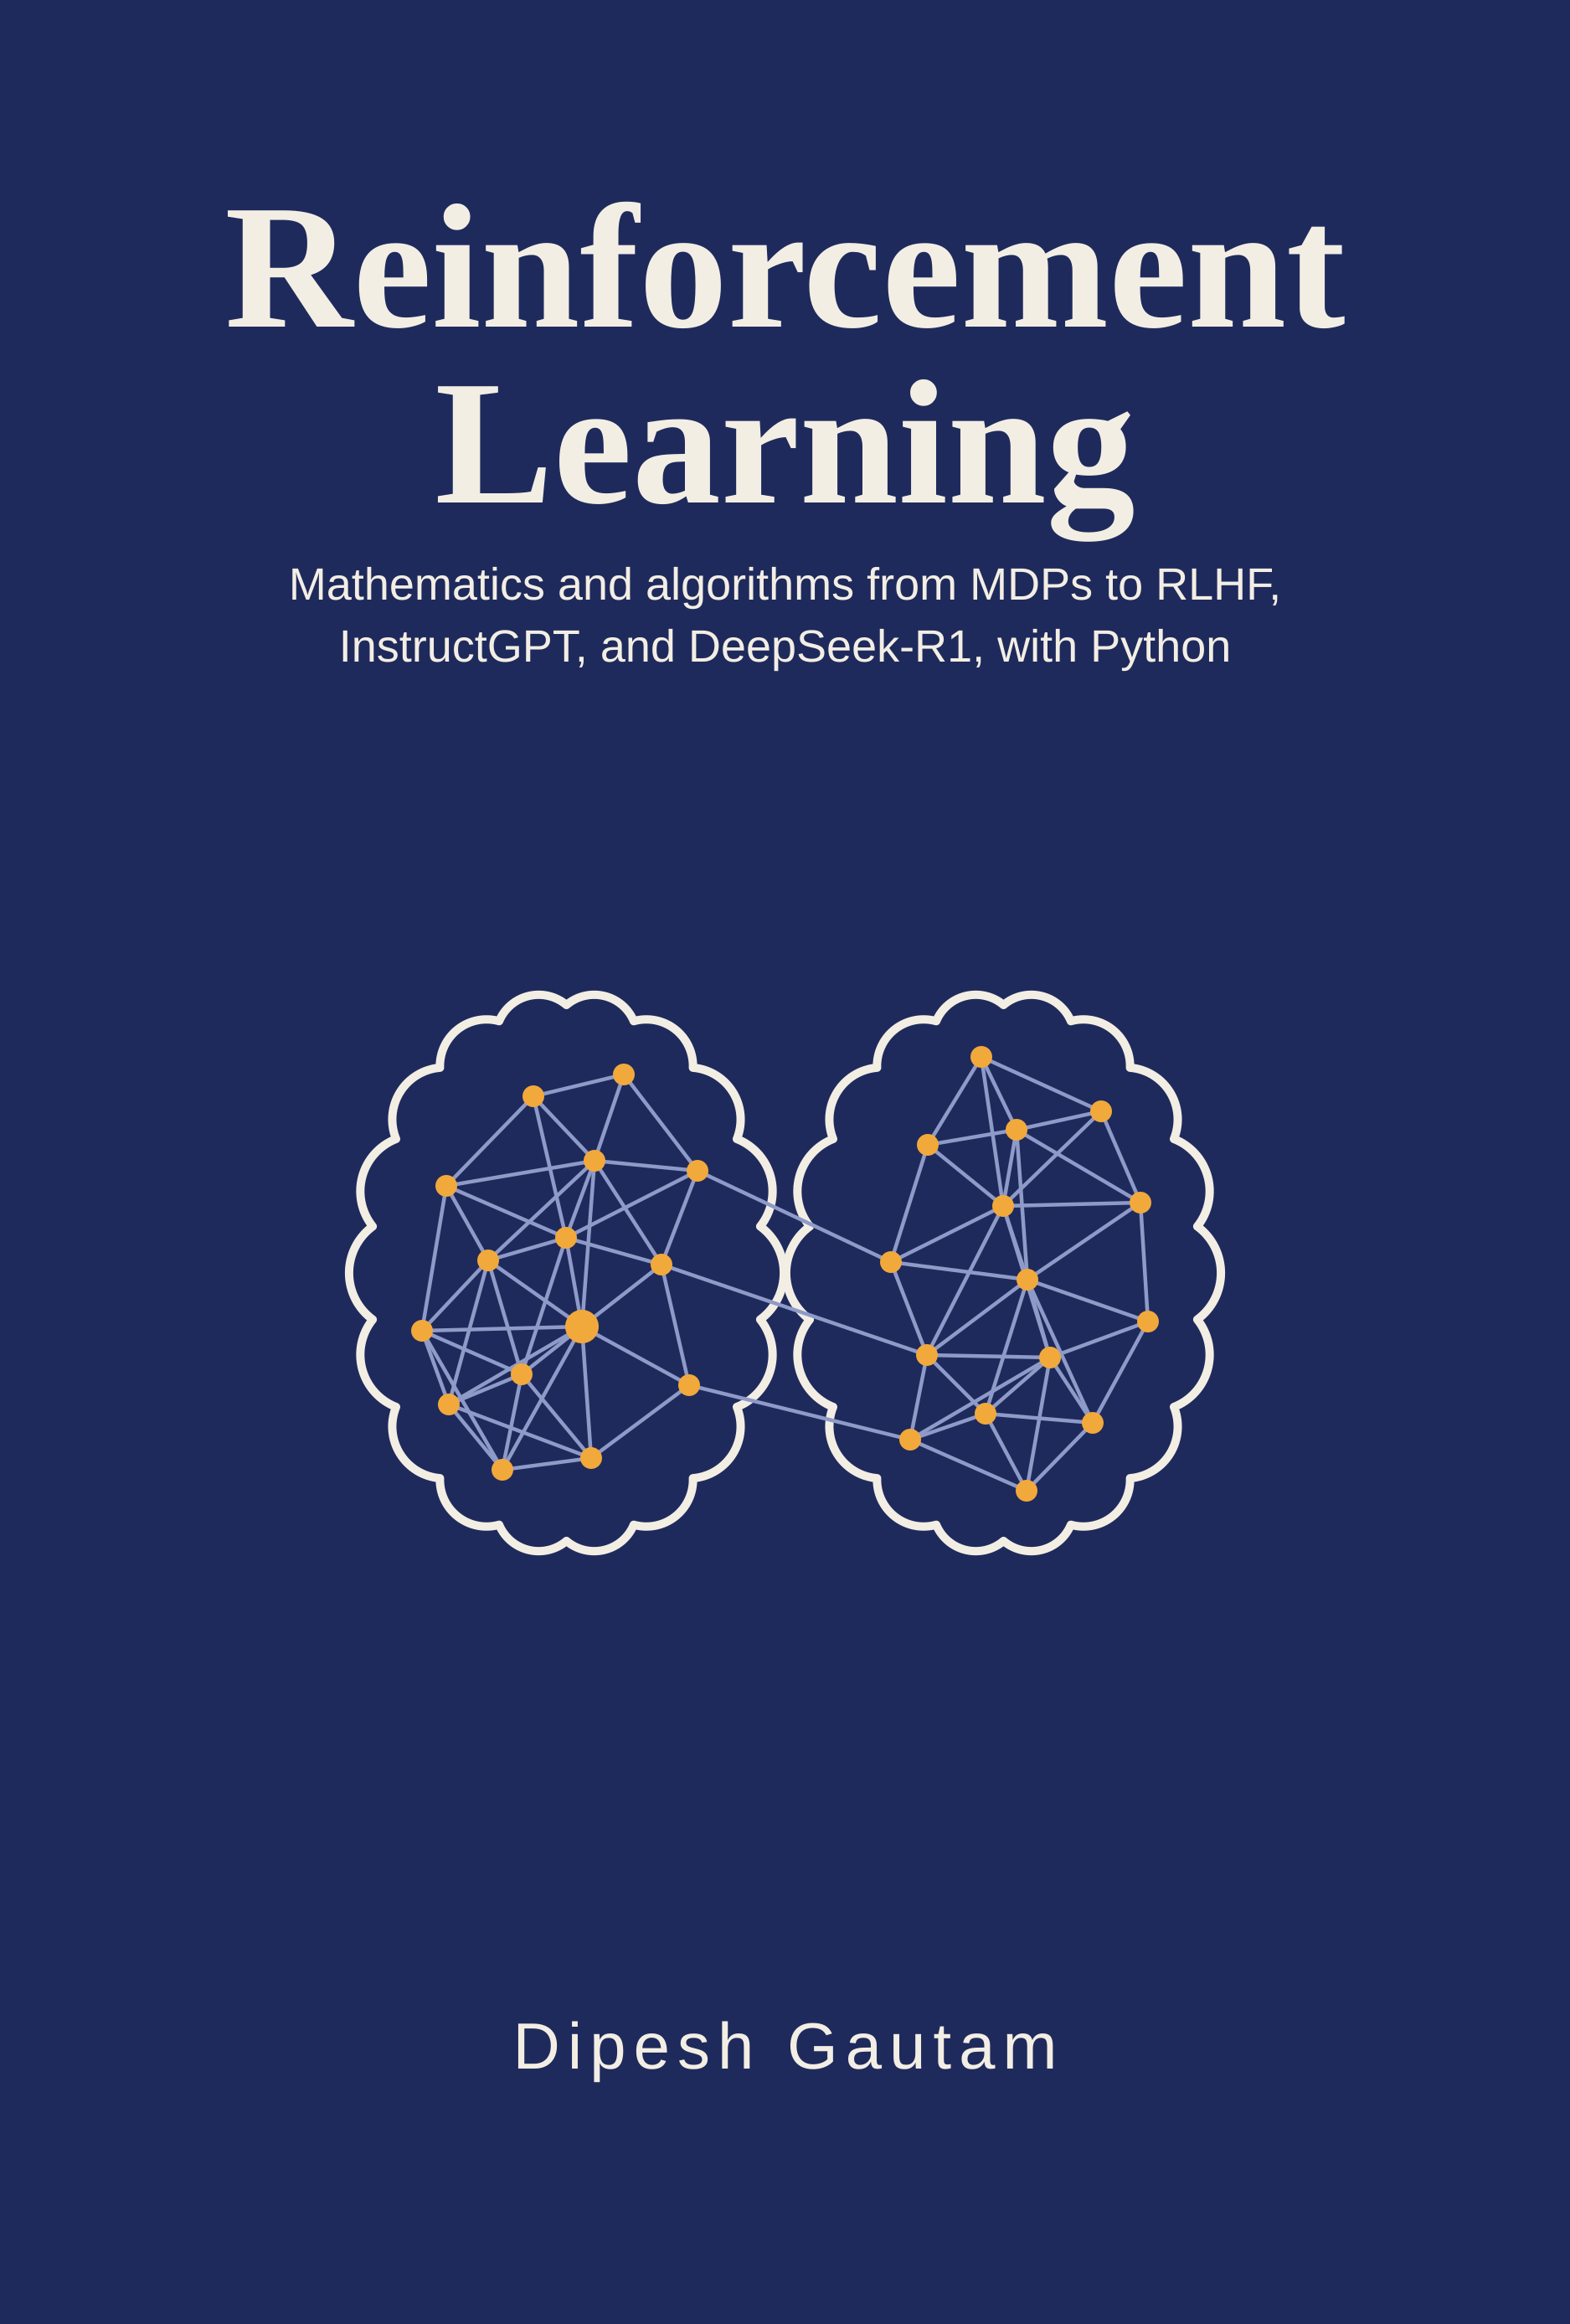
\includegraphics[width=\paperwidth,height=\paperheight]{book_cover.png}}}%
\null
\clearpage
\maketitle
\chapter*{Disclaimer}
This book derives standard reinforcement learning methods and writes Python for the same updates. The algorithms, theorems, and named systems are due to the works listed in the References. It does not introduce a new algorithm. Chapters 11 and 12 describe the shape of InstructGPT-style and DeepSeek-R1-style training; they do not train those published systems, and they do not use their models, data, or infrastructure.

\textbf{Generative artificial intelligence tools were utilized to refine the prose explanations of these standard methods and optimize their linguistic flow. The final text, overarching structure, and conceptual curation were executed by the author. All mathematical derivations, algorithmic loops, and Python source code listings have been manually cross-verified against primary literature by the author, who assumes sole responsibility for the technical correctness, accuracy, and integrity of the final work.}
\tableofcontents
\chapter{Preface}

This book presents reinforcement learning through the relations that define the problem, the derivations of those relations, the algorithms that apply them, and short Python programs that follow the same steps. It is intended for readers who know basic probability and statistics and who can read Python. A previous course in reinforcement learning is not required.

Each method begins with the object to be learned. The compact equation is stated next. When that equation abbreviates a longer expansion, the expansion is derived in the chapter or in an appendix from the probability identities in Appendix A, which are cited by number. The algorithm then records the update as a loop. A Python listing on a small environment follows that loop in the same section.

Appendix A contains the facts used later, including total probability, expectation, variance, importance sampling, and the Markov property. Those facts may be read first, or Chapter 1 may be started at once and the appendix consulted when an identity is cited. Longer derivations that would interrupt a chapter are placed in later appendices. They include the Bellman expansions, the Robbins--Monro step-size conditions, the policy-gradient theorem, and the non-negativity of KL, and they use the same identities as Appendix A.

The chapters treat Markov decision processes and the Bellman equations, dynamic programming, Monte Carlo methods, temporal-difference learning and control, function approximation, deep Q-networks, policy gradients, and actor--critic methods, and then reinforcement learning from human feedback together with InstructGPT-style and DeepSeek-R1-style training. A summary collects the objects. The algorithms, theorems, and named systems are those of the works listed in the References. The text is not a research monograph.

Each algorithm in the main chapters is accompanied by a program on a small state set. The listing stands next to the boxed steps so that one update can be read as a program. Two exercises at the end of the book apply several methods to one environment. The first is a $4\times 4$ GridWorld under value iteration, Monte Carlo control, SARSA, and Q-learning. The second is CartPole with a deep Q-network. Solutions are given. Chapters 11 and 12 use a language-model example with checkable answers. They describe the shape of InstructGPT-style and DeepSeek-R1-style training and do not train the published systems.

\mainmatter
\chapter{The RL Problem: MDPs, Policies, and Returns}

Machine learning produces a rule from data. The usual case is \textbf{supervised learning}, a fixed set of pairs $(x,y)$ where the task is to predict $y$ from $x$. An image labeled ``cat,'' a prompt paired with a gold reply---each example already names the correct output. Training compares the model's output to that label. That is the right tool when the right answer is known for each input.

It does not apply when we must choose actions over time and the data do not include the correct action at each step. For example, balancing a pole, playing chess, or writing a reply that is scored only when it is finished: no $(\text{state},\,\text{correct action})$ pairs are available, and the agent has to learn from interaction with the environment. After each action the agent sees a scalar \textbf{reward}, which may arrive much later than the choice that caused it. The signal does not tell which earlier action was responsible. \textbf{Reinforcement learning} is the problem of producing \textbf{good trajectories}---sequences of states, actions, and rewards with high total reward---not a single labeled output.

A large reward now can still leave the rest of the sequence poor; a reward that looks poor now can be required for a later win. So a single reward is not a grade of the action. The object to judge is the whole trajectory. For example, in chess, a sacrifice on move 10 may yield no immediate reward, yet be the reason for checkmate on move 40. If move 10 were scored only by the material lost that turn, the sacrifice would look like a mistake.

A trajectory is a sequence of choices, so the rule we search for is not one labeled output but a \textbf{policy} $\pi$: given the current state, which action to take. What follows is how an agent and an environment interact, the Markov decision process, and the \textbf{return} $G_t$ that scores a trajectory from time $t$. Later chapters find a $\pi$ that makes that return large.

\section{Interaction and policy}
The interaction has two sides. The \textbf{agent} chooses actions. The \textbf{environment} presents a situation and, after the action, replies with a new situation and a scalar reward.

For example, if a taxi driver must choose a turn at each junction without a labeled correct turn, the driver is the agent and the city is the environment. At a junction the driver sees the intersection---the \textbf{state}---and takes a turn: left, straight, or right---the \textbf{action}. The city replies with the next intersection---the \textbf{next state}---and a fare or a time penalty---the \textbf{reward}. The fare or the time penalty is the feedback: not a labeled correct turn, and it may arrive later in the trip.

The same exchange happens at every junction. Index those steps by a discrete time $t = 0, 1, 2, \dots$:

\begin{enumerate}
\item \textbf{State Observation:} Agent observes state $S_t \in \mathcal{S}$.
\item \textbf{Action Selection:} Agent executes action $A_t \in \mathcal{A}$.
\item \textbf{Environment Response:} Environment transitions to state $S_{t+1} \in \mathcal{S}$ and emits scalar reward $R_{t+1} \in \mathbb{R}$.
\item \textbf{Learning Step:} Agent updates its policy or value estimates based on $(S_t, A_t, R_{t+1}, S_{t+1})$.
\end{enumerate}
\[
S_t \xrightarrow{A_t} (S_{t+1}, R_{t+1}) \xrightarrow{A_{t+1}} (S_{t+2}, R_{t+2}) \rightarrow \cdots
\]

The rule in step 2 is the \textbf{policy} $\pi$: given the current junction, which turn to take. It is only that turn-taking rule---not the layout of the streets, and not the fare. Even if two trips start at the same junction, the driver may take a different turn, because the environment is not deterministic: a road may be closed, or traffic may block a street.

The policy is how the driver chooses among the turns that are still legal. If left, straight, and right are all open, the rule can leave more than one of them possible. If the light is red, the only legal action is to wait, so the rule is the same on every visit. Those two cases are:

\begin{itemize}
\item \textbf{Stochastic policy $\pi(a \mid s)$.} A distribution over actions in a state:
\end{itemize}
\[
\pi(a \mid s) = P(A_t = a \mid S_t = s), \quad \sum_{a \in \mathcal{A}} \pi(a \mid s) = 1.
\] Two visits to an open junction can then take different roads.

\begin{itemize}
\item \textbf{Deterministic policy $\pi(s)$.} A fixed map from state to one action:
\end{itemize}
\[
a = \pi(s).
\] At a red light that is $\pi(\text{red light})=\text{wait}$ on every visit.

\section{The Markov decision process}
A trajectory is the sequence

\[
S_0,\; A_0,\; R_1,\; S_1,\; A_1,\; R_2,\; S_2,\; \ldots
\]

We cannot usually write down one frozen sequence in advance. After each action the environment replies with a next state and reward, and that reply can be random: the taxi takes a left at the same junction and, depending on construction or traffic, reaches a different street. The policy of Section 1.1 selects the action at each state; the environment replies with $(s',r)$.

The same left turn can lead to a different $s'$ if the avenue is closed, so the pair $(s', r)$ is random. What it does \textit{not} depend on is the long list of earlier streets: given this junction and this turn, the past route is irrelevant. That is the \textbf{Markov} property. It is a Markov \textbf{decision} process, not only a Markov chain, because the agent chooses $a$ at every state.

Four objects define it: the states, the actions, the transition probability $P$, and a discount $\gamma$ that weights immediate rewards against future rewards. An MDP is the tuple $(\mathcal{S}, \mathcal{A}, P, \gamma)$:

\begin{center}
\begin{tabular}{ll}
\toprule
Symbol & Definition \\
\midrule
$\mathcal{S}$ & Set of all valid states (state space) \\
$\mathcal{A}$ & Set of all valid actions (action space) \\
$P$ & Transition probability (next state and immediate reward) \\
$\gamma \in [0, 1]$ & Discount factor weighting future rewards vs. immediate rewards \\
\bottomrule
\end{tabular}
\end{center}

$\mathcal{S}$ and $\mathcal{A}$ are the agent's interface. What remains is $P$: the probability of the next state and reward after the agent acts. In full generality that probability could depend on the entire past,

\[
P(S_{t+1}, R_{t+1} \mid S_t, A_t, S_{t-1}, A_{t-1}, \dots, S_0, A_0).
\]

Carrying every previous intersection, turn, and fare is unusable. If construction, traffic, and layout at \textit{this} junction already sit in $S_t$, then older decisions add nothing. The same left turn from the same junction has the same distribution over $(S_{t+1}, R_{t+1})$ whether the taxi arrived from the north or the east. That is the \textbf{Markov property}. Given the present state and the action just chosen, the future is independent of the past.

\begin{equation}
P(S_{t+1}, R_{t+1} \mid S_t, A_t, S_{t-1}, A_{t-1}, \dots, S_0, A_0)
=
P(S_{t+1}, R_{t+1} \mid S_t, A_t). \tag{1.1}
\end{equation}

Under (1.1) the environment depends on the agent only through the current state and action. Write lowercase $s \in \mathcal{S}$, $a \in \mathcal{A}$, $s' \in \mathcal{S}$, and $r \in \mathbb{R}$ for particular values of the random variables $S_t$, $A_t$, $S_{t+1}$, and $R_{t+1}$. The transition probability is therefore

\begin{equation}
P(s',r \mid s,a)
=
P\!\left(S_{t+1}=s',\, R_{t+1}=r \mid S_t=s,\, A_t=a\right). \tag{1.2}
\end{equation}

The pair $(s', r)$ is joint because the next state and the immediate reward often come together---arriving at a destination, for example, both changes the state and yields a reward. Together with the policy $\pi(a \mid s)$, (1.2) generates the trajectory: the agent chooses $A_t$ from $\pi$, then the environment draws $(S_{t+1}, R_{t+1})$ from $P$. From here on, statements about the environment use $P(s',r \mid s,a)$.

\section{Rewards and next-state probabilities}

Equation (1.2) is the joint of one next junction and one fare. From a junction several turns may be legal, and each continuation can yield a different fare; we want the expected fare from that state. The same turn can also lead to different next junctions; we want the probability of arriving at a particular junction. Both of those, and then the same quantities averaged under $\pi$, come from $P(s',r\mid s,a)$. Derivations of the expected-reward identities are in \appref{B}.

\textbf{Where the taxi goes.} The joint $P(s',r\mid s,a)$ is the probability of reaching next state $s'$ together with each possible fare (reward) $r$. The probability of being in $s'$ after the turn is the total of those probabilities over every fare:

\begin{equation}
P(s' \mid s,a) = \sum_{r} P(s',r \mid s,a)
\quad\text{[law of total probability]}
\tag{1.3}
\end{equation}

\textbf{What fare to expect, given also the next junction.} The expected fare given this junction, this turn, and arrival at $s'$ is

\begin{equation}
R(s,a,s')
=
\mathbb{E}[R_{t+1} \mid S_t=s, A_t=a, S_{t+1}=s']
=
\sum_{r} r\, \frac{P(s',r \mid s,a)}{P(s' \mid s,a)}.
\tag{1.4}
\end{equation}

So $R(s,a,s')$ is the expected immediate reward from taking action $a$ in state $s$ and arriving at $s'$ (\appref{B}, \eqref{eq:B.4}).

\textbf{What fare to expect for this turn.} If the next junction is not fixed, average the immediate reward given only $(s,a)$:

\begin{equation}
R(s,a)
=
\mathbb{E}[R_{t+1} \mid S_t=s, A_t=a]
=
\sum_{s',r} r\, P(s',r \mid s,a)
=
\sum_{s'} P(s' \mid s,a)\, R(s,a,s').
\tag{1.5}
\end{equation}

So $R(s,a)$ is the expected immediate reward from taking action $a$ in state $s$ (\appref{B}, \eqref{eq:B.5}). The last equality averages $R(s,a,s')$ over the next-state distribution (1.3).

\textbf{When $\pi$ chooses the action.} The agent no longer fixes $a$; at state $s$ it chooses actions according to $\pi(a\mid s)$. Averaging under $\pi$ gives the expected reward from $s$ and the next-state probability from $s$ under that policy:

\begin{equation}
R^\pi(s)
=
\mathbb{E}_\pi[R_{t+1} \mid S_t=s]
=
\sum_a \pi(a \mid s)\, R(s,a)
=
\sum_a \pi(a \mid s) \sum_{s',r} r\, P(s',r \mid s,a),
\tag{1.6}
\end{equation}

\begin{equation}
P^\pi(s' \mid s)
=
\sum_a \pi(a \mid s)\, P(s' \mid s,a)
\quad\text{[law of total probability]}
\tag{1.7}
\end{equation}

So $R^\pi(s)$ is the expected immediate reward from $s$ under $\pi$ (\appref{B}, \eqref{eq:B.12}), and $P^\pi(s'\mid s)$ is the probability of moving from $s$ to $s'$ under $\pi$. Those quantities are stacked into a vector and a matrix in Chapter 2, for one fixed policy.

\section{Return and discounting}
The previous sections stated the goal: find a policy that produces good trajectories. We now say what ``good'' means. The quality of a trajectory from time $t$ is the \textbf{return} $G_t$: a single number that combines all future rewards along that trajectory.

Rewards at different times are not treated as equal. A fare collected now is worth more than the same fare many turns later---the taxi may finish the shift, traffic may change, or we simply prefer money sooner. \textbf{Discounting} encodes that preference with a factor $\gamma \in [0,1]$. A reward $k$ steps ahead is scaled by $\gamma^k$, so later rewards shrink (unless $\gamma=1$).

Without discounting, the infinite sum $\sum_{k=0}^\infty R_{t+k+1}$ can diverge even when every reward is bounded. With $\gamma \in [0,1)$, the geometric weights force the sum to converge, and they also express ``sooner is better'':

\begin{equation}
G_t
=
\sum_{k=0}^{\infty} \gamma^k R_{t+k+1}
=
R_{t+1} + \gamma R_{t+2} + \gamma^2 R_{t+3} + \cdots.
\tag{1.8}
\end{equation}

So $R_{t+1}$ enters at full weight, $R_{t+2}$ at weight $\gamma$, $R_{t+3}$ at $\gamma^2$, and so on.

\begin{itemize}
\item If $\gamma=0$, only the immediate reward matters: $G_t=R_{t+1}$.
\item If $\gamma$ is close to $1$, distant rewards still count almost as much as near ones.
\item If $\gamma=1$, there is no discounting; that is usable mainly for episodic tasks that stop at a finite horizon $T$:
\end{itemize}
\begin{equation}
G_t = \sum_{k=0}^{T-t-1} \gamma^k R_{t+k+1}.
\tag{1.9}
\end{equation}

The infinite sum (1.8) rewrites by factoring $\gamma$ from every term after the first:

\[
\begin{aligned}
G_t
&= R_{t+1} + \gamma R_{t+2} + \gamma^2 R_{t+3} + \gamma^3 R_{t+4} + \cdots \\
&= R_{t+1} + \gamma \left( R_{t+2} + \gamma R_{t+3} + \gamma^2 R_{t+4} + \cdots \right) \\
&= R_{t+1} + \gamma G_{t+1}.
\end{aligned}
\]

The recursive form is therefore

\begin{equation}
G_t = R_{t+1} + \gamma G_{t+1}.
\tag{1.10}
\end{equation}

So the return is the immediate reward plus a discounted copy of the return from the next time. That identity is what value functions will average in the next chapter.

\chapter{Value Functions and the Bellman Equations}

The return $G_t$ scores a trajectory. The interaction is an MDP: the policy $\pi$ selects the action; the environment replies with $(s',r)$ from $P$. That return is one number for one realized sequence. Take the taxi introduced in Chapter 1: from a junction it still faces many possible futures. The policy $\pi$ may leave more than one turn possible, and $P$ may send it to different streets with different fares. Two trips that start at the same junction can therefore finish with different returns: $G_t$ from that junction is a random variable. One realized return does not tell how good the junction is.

To say how good that junction is under a fixed $\pi$, take the expected return from there: the \textbf{state-value} $V^\pi$. To say how good a particular turn is, take the expected return after that turn: the \textbf{action-value} $Q^\pi$. Both are rewritten as \textbf{Bellman equations} (\citetxt{bellman1957}{Bellman, 1957}) that use only the immediate reward and the value at the next state. Averaging over $\pi$ \textbf{evaluates} that policy. Replacing the average by $\max_a$ is optimality: the rewrite that \textbf{improves} $\pi$.

The expected return from $s$ when actions afterward follow $\pi$ is the \textbf{state-value} $V^\pi(s)$.

\begin{equation}
V^\pi(s) = \mathbb{E}_\pi [G_t \mid S_t = s].
\tag{2.1}
\end{equation}

We also care how good a particular turn $a$ is at that junction. Fix $A_t=a$, then follow $\pi$ from the next state on: the expected return is the \textbf{action-value} $Q^\pi(s,a)$.

\begin{equation}
Q^\pi(s,a) = \mathbb{E}_\pi [G_t \mid S_t = s, A_t = a].
\tag{2.2}
\end{equation}

\section{Bellman expectation equations}
$V^\pi(s)$ is an expected return, and the return is an infinite discounted sum of future rewards. Computing that expectation by listing every possible future under $\pi$ and $P$ is not practical. Using $G_t=R_{t+1}+\gamma G_{t+1}$ in the definition of $V^\pi$, the Bellman expectation equation is obtained as follows.

\[
\begin{aligned}
V^\pi(s)
&= \mathbb{E}_\pi [G_t \mid S_t = s] \\
&= \mathbb{E}_\pi [R_{t+1} + \gamma G_{t+1} \mid S_t = s] \\
&= \mathbb{E}_\pi [R_{t+1} \mid S_t = s] + \gamma \mathbb{E}_\pi [G_{t+1} \mid S_t = s].
\end{aligned}
\]

So

\begin{equation}
V^\pi(s)
=
\mathbb{E}_\pi [R_{t+1} \mid S_t = s]
+
\gamma\, \mathbb{E}_\pi [G_{t+1} \mid S_t = s].
\tag{2.3}
\end{equation}

The first term is the expected immediate reward from $s$ under $\pi$. The second is the expected value of the next state, again under $\pi$. Expanding both over $\pi(a\mid s)$ and $P(s',r\mid s,a)$ is in \appref{B}, \eqref{eq:B.1}. The result is

\begin{equation}
V^\pi(s) = \sum_{a \in \mathcal{A}} \pi(a \mid s) \sum_{s', r} P(s',r \mid s,a) \left[ r + \gamma V^\pi(s') \right].
\tag{2.4}
\end{equation}

The inner piece $r+\gamma V^\pi(s')$ looks only one step ahead: $r$ is the immediate reward on the transition to $s'$ (a value of $R_{t+1}$), and $V^\pi(s')$ is the value at the next state. That one-step rewrite is a \textbf{backup}.

Equation (2.4) nests two averages---over actions under $\pi$, then over transitions under $P$. These are the same as $V^\pi$ through $Q^\pi$ (\appref{B}, \eqref{eq:B.14} and \eqref{eq:B.17}):

\[
V^\pi(s)
=
\sum_{a \in \mathcal{A}}
\pi(a \mid s)\, Q^\pi(s,a),
\qquad
Q^\pi(s,a)
=
\sum_{s',r}
P(s',r \mid s,a)
\bigl[
r + \gamma V^\pi(s')
\bigr].
\]

So the outer sum in (2.4) averages over actions under $\pi$, and the inner sum averages over the next state and reward under $P$.

Starting from $Q^\pi(s,a)$ and eliminating $V^\pi$ at the next state (\appref{B}, \eqref{eq:B.2}) gives

\begin{equation}
Q^\pi(s,a) = \sum_{s',r} P(s',r \mid s,a) \left[ r + \gamma \sum_{a'} \pi(a' \mid s') Q^\pi(s',a') \right].
\tag{2.5}
\end{equation}

\subsection{Matrix form}
The policy-averaged form of $V^\pi$ (\appref{B}, \eqref{eq:B.3}) is

\[
V^\pi(s)
=
R^\pi(s)
+
\gamma
\sum_{s'}
P^\pi(s' \mid s)\, V^\pi(s'),
\]

with $R^\pi$ and $P^\pi$ as in Section 1.3. For a finite state space of size $N$, stack $V^\pi(s)$ into a vector $\mathbf{V}^\pi\in\mathbb{R}^N$, stack $R^\pi(s)$ into $\mathbf{R}^\pi$, and let $\mathbf{P}^\pi$ be the $N\times N$ matrix with entry $(s,s')$ equal to $P^\pi(s'\mid s)$. The display above for every $s$ is the single matrix equation

\[
\mathbf{V}^\pi = \mathbf{R}^\pi + \gamma \mathbf{P}^\pi \mathbf{V}^\pi.
\]

Solve for $\mathbf{V}^\pi$:

\begin{equation}
\mathbf{V}^\pi - \gamma \mathbf{P}^\pi \mathbf{V}^\pi = \mathbf{R}^\pi
\implies
(I - \gamma \mathbf{P}^\pi)\mathbf{V}^\pi = \mathbf{R}^\pi
\implies
\mathbf{V}^\pi = (I - \gamma \mathbf{P}^\pi)^{-1} \mathbf{R}^\pi.
\tag{2.6}
\end{equation}

For $\gamma\in[0,1)$, $I-\gamma\mathbf{P}^\pi$ is invertible, so evaluating $\pi$ is one linear solve---not an iteration.

\begin{asidenote}[Note]
A two-junction taxi makes the arrays concrete. The states are the depot $D$ and the street $S$. Under $\pi$ the taxi always leaves the depot for the street (immediate reward $0$). From the street it collects a fare of $1$ and returns to the depot with probability $1/2$, or stays on the street with reward $0$ with probability $1/2$. Then

\[
\mathbf{P}^\pi
=
\begin{bmatrix}
0 & 1 \\
\tfrac{1}{2} & \tfrac{1}{2}
\end{bmatrix},
\qquad
\mathbf{R}^\pi
=
\begin{bmatrix}
0 \\
\tfrac{1}{2}
\end{bmatrix},
\]

with rows and columns ordered $(D,S)$. Take $\gamma=1/2$. The two scalar copies of (2.4) are

\[
\begin{aligned}
V^\pi(D)
&=
0 + \tfrac{1}{2} V^\pi(S), \\
V^\pi(S)
&=
\tfrac{1}{2} + \tfrac{1}{2}
\bigl(
\tfrac{1}{2} V^\pi(D) + \tfrac{1}{2} V^\pi(S)
\bigr).
\end{aligned}
\]

The same system is (2.6):

\[
I - \gamma \mathbf{P}^\pi
=
\begin{bmatrix}
1 & -\tfrac{1}{2} \\
-\tfrac{1}{4} & \tfrac{3}{4}
\end{bmatrix},
\qquad
\mathbf{V}^\pi
=
(I - \gamma \mathbf{P}^\pi)^{-1} \mathbf{R}^\pi
=
\begin{bmatrix}
\tfrac{2}{5} \\
\tfrac{4}{5}
\end{bmatrix}.
\]

So $V^\pi(D)=2/5$ and $V^\pi(S)=4/5$. Substituting back into $\mathbf{R}^\pi+\gamma\mathbf{P}^\pi\mathbf{V}^\pi$ recovers the same vector.
\end{asidenote}

\section{Bellman optimality equations}
The Bellman expectation equations are for one fixed $\pi$. We now want values that are best in every state: the \textbf{optimal} state-value and action-value

\begin{equation}
V^*(s) = \max_\pi V^\pi(s),
\qquad
Q^*(s,a) = \max_\pi Q^\pi(s,a).
\tag{2.7}
\end{equation}

Under an optimal policy the agent no longer averages actions with $\pi(a\mid s)$; it takes an action that attains the maximum. The same one-step backup as (2.4), with that $\max$ in place of the average over $\pi$, is the \textbf{Bellman optimality equation} (\appref{C}, \eqref{eq:C.2}):

\begin{equation}
V^*(s) = \max_{a \in \mathcal{A}} \sum_{s',r} P(s',r \mid s,a) \left[ r + \gamma V^*(s') \right].
\tag{2.8}
\end{equation}

The $\max$ means: score every action by that sum and keep the best. That is only possible once the next-state values $V^*(s')$ are known; those values depend on other states the same way, so (2.8) couples the whole table and does not yield $V^*$ by one pass of ``try every $a$.''

\begin{equation}
Q^*(s,a) = \sum_{s',r} P(s',r \mid s,a) \left[ r + \gamma \max_{a'} Q^*(s',a') \right].
\tag{2.9}
\end{equation}

From (2.8), an optimal policy is greedy on those one-step scores:

\begin{equation}
\pi^*(s)
=
\arg\max_{a \in \mathcal{A}}
\sum_{s',r}
P(s',r \mid s,a)
\left[
r + \gamma V^*(s')
\right].
\tag{2.10}
\end{equation}

That choice uses $P$ even after $V^*$ is known. Computing $Q^*$ from (2.9) also uses $P$. Once the table $Q^*$ is known, the same policy is an $\arg\max$ over $a$ and does not use $P$:

\begin{equation}
\pi^*(s) = \arg\max_{a \in \mathcal{A}} Q^*(s,a).
\tag{2.11}
\end{equation}

The $\arg\max$ can contain more than one action: two turns with the same score. A greedy $\pi^*$ always takes one of them. Randomizing between those two is also optimal. Taking a turn whose score is strictly smaller is not (\appref{C}, \hyperref[app:C.4]{C.4}).

Equations (2.4)--(2.6) are linear in $V^\pi$, so a fixed policy is one matrix solve; (2.8)--(2.9) contain a $\max$, so that solve no longer applies and $V^*$ needs iteration (Chapter 3).

\chapter{Dynamic Programming}

When the model $P$ is known, the Bellman equations are two computations: obtain $V^\pi$ for a given $\pi$, and obtain $V^*$ (and a $\pi^*$). The first obtains $V^\pi$, the expected return from each state under a given $\pi$, and is therefore called \textbf{prediction}. The second finds a $\pi^*$ that chooses, at each state, an action that maximizes expected return, and is therefore called \textbf{control}. $V^*$ is the value of that policy.

For a \textit{fixed} policy $\pi$, the Bellman expectation equation is linear in the unknowns $V^\pi(s)$. In matrix form that is $\mathbf{V}^\pi=\mathbf{R}^\pi+\gamma\mathbf{P}^\pi\mathbf{V}^\pi$, which rearranges to the linear solve (2.6):

\[
\mathbf{V}^\pi=(I-\gamma\mathbf{P}^\pi)^{-1}\mathbf{R}^\pi.
\]

One solve gives every $V^\pi(s)$ at once. No iteration is required.

For the \textit{optimal} values $V^*$, the Bellman optimality equation (2.8) has a $\max$ over actions. That $\max$ makes the system nonlinear, so the same matrix rearrange and solve no longer applies. At one state, the $\max$ only compares action scores---and each score still needs $V^*(s')$ at the next states, which are unknown and coupled across the whole table. Trying every $a$ at one state therefore cannot produce $V^*$ in a single pass.

Dynamic programming (DP) iterates the second computation: when $P$ is known, apply (2.8) over all states repeatedly until the value table converges to $V^*$. That iteration replaces the linear solve we had for $V^\pi$.

Two standard DP algorithms do this:

\begin{itemize}
\item \textbf{Value iteration} updates the value table by repeatedly applying (2.8) until it converges to $V^*$, then reads off a greedy policy (Section 3.1).
\item \textbf{Policy iteration} alternates \textit{policy evaluation} and \textit{policy improvement} until the policy stops changing (Section 3.2).
\end{itemize}
Both need the model $P$. If $P$ is unknown, DP does not apply; later chapters use sample-based methods instead (Monte Carlo, then TD), which learn from experience rather than from summing over $P$.

\section{Value Iteration}
Value iteration computes $V^*$ by repeatedly applying (2.8), then a greedy $\pi^*$. On non-terminal states the starting table $V_0$ may be any guess; the updates still converge. After a terminal state there are no further rewards, so the return from there is $0$. Those entries stay at $V(\text{terminal})=0$ and are not updated. Each round then updates every non-terminal value by (2.8) on the current table $V_k$. The policy at $s$ is (2.10) on that same table:

\begin{equation}
\begin{aligned}
V_{k+1}(s)
&
\leftarrow
\max_{a} \sum_{s',r} P(s',r \mid s,a) \left[ r + \gamma V_k(s') \right],
\\
\pi_{k+1}(s)
&
\leftarrow
\arg\max_{a} \sum_{s',r} P(s',r \mid s,a) \left[ r + \gamma V_k(s') \right].
\end{aligned}
\tag{3.1}
\end{equation}

Equation (3.1) uses the previous-round table $V_k$ at every next state $s'$, for both $V_{k+1}$ and $\pi_{k+1}$. The algorithm below writes the new number into $V(s)$ before moving to the next state in the loop, so a later state's value and action may already read that new $V(s)$. Repeating this backup still improves the table: an early $V_k$ is only a guess, a later $V_k$ is closer to $V^*$. For $\gamma\in[0,1)$, $V_k$ converges to $V^*$, and the greedy $\pi_k$ at that limit is an approximate $\pi^*$. Exact $V^*$ is a limit of infinitely many sweeps. In practice one sweep records $\Delta$, the largest $|V(s)-v|$ over the non-terminals just updated, and stops when $\Delta<\varepsilon$ for a chosen tolerance $\varepsilon>0$.

\begin{figure}[ht]
\centering
\setlength{\fboxsep}{5pt}%
\setlength{\fboxrule}{0.4pt}%
{\color{black!30}\fbox{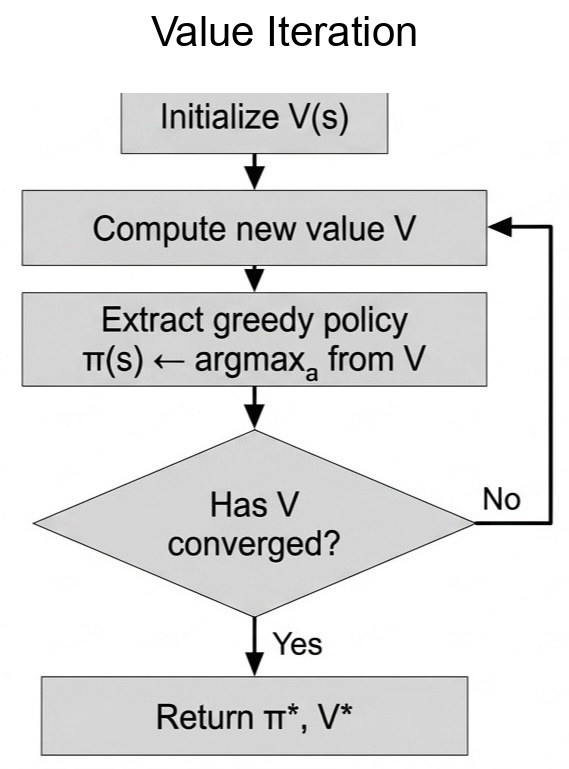
\includegraphics[width=0.46\textwidth]{value_iteration_cycle.jpeg}}}
\caption{Value iteration.}\label{fig-5-1}
\end{figure}

\begin{implnote}[Algorithm (value iteration)]
Input: model $P(s',r\mid s,a)$ and tolerance $\varepsilon>0$.

Output: $V\approx V^*$ and greedy $\pi\approx\pi^*$.

\begin{enumerate}
\item Choose any initial $V(s)$ for non-terminal states; set $V(s)\leftarrow 0$ for terminals and leave them fixed.
\item Repeat:
\begin{itemize}
\item $\Delta\leftarrow 0$.
\item For each non-terminal state $s$:
\begin{itemize}
\item $v\leftarrow V(s)$.
\item $V(s)\leftarrow\max_a\sum_{s',r} P(s',r\mid s,a)\,[r+\gamma V(s')]$.
\item $\pi(s)\leftarrow\arg\max_a\sum_{s',r} P(s',r\mid s,a)\,[r+\gamma V(s')]$.
\item $\Delta\leftarrow\max(\Delta,|v-V(s)|)$.
\end{itemize}
\item Stop if $\Delta<\varepsilon$.
\end{itemize}
\item Return $V$ and $\pi$ (use $\pi$ only after this stop).
\end{enumerate}

\end{implnote}

\lstinputlisting{../code/ch03/value_iteration.py}


\section{Policy Iteration}
Policy iteration also computes $V^*$ and $\pi^*$ when $P$ is known. Unlike value iteration, it does not take $\max$ inside every value update: a policy $\pi$ is held fixed while $V^\pi$ is computed, then $\pi$ is replaced by a greedy policy from that $V^\pi$. Terminals stay at $V=0$ and are not updated.

The process is:
\begin{enumerate}
\item Start with any policy $\pi$ (e.g. random).
\item With $\pi$ fixed, compute $V^\pi$ by repeatedly updating $V$ until $V$ converges.
\item From that $V^\pi$, build a new greedy policy $\pi'$.
\item If $\pi'=\pi$, stop: $\pi$ is optimal and $V^\pi=V^*$. Else set $\pi\leftarrow\pi'$ and go back to step 2 (new $V$ under the new policy, then a new greedy policy, and so on).
\end{enumerate}
Each time the policy changes, $V$ must be recomputed for that policy. The process stops when the \textbf{policy} stops changing.

\begin{figure}[ht]
\centering
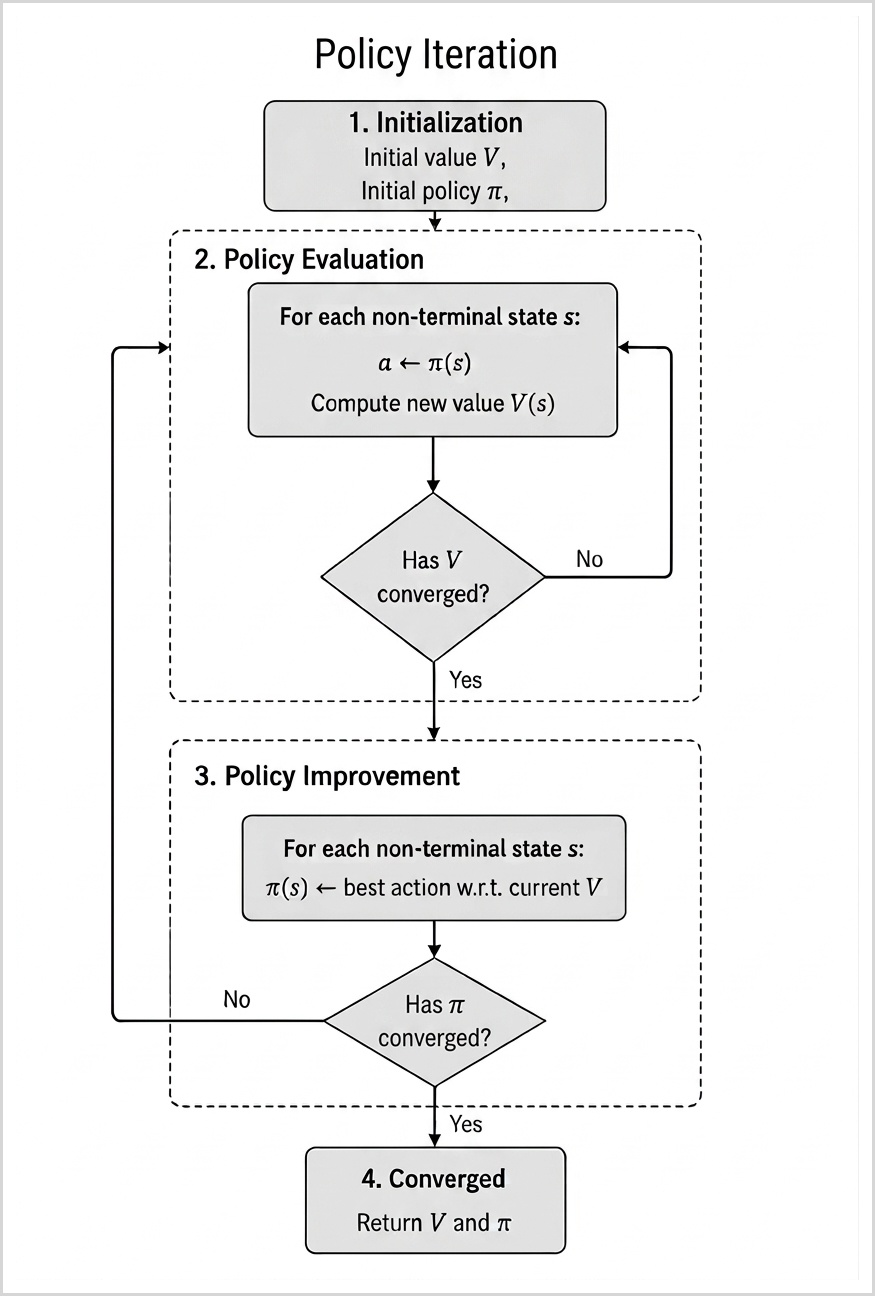
\includegraphics[width=0.62\textwidth]{policy_iteration_cycle.jpeg}
\caption{Policy iteration.}\label{fig-5-2}
\end{figure}

Policy evaluation computes $V^\pi$ for a fixed $\pi$, the expected return from each state if the agent keeps following $\pi$. It does not yet change $\pi$.

With one action $a=\pi(s)$ at each $s$, there is no $\max$, so the Bellman expectation equation is linear in $V^\pi$, unlike (3.1). Equation (2.6) solves that system by one matrix inverse. When there are many states the inverse is expensive, so the algorithm below instead repeats the one-step backup over non-terminals until $V$ settles. That inner stop is the same $\Delta<\varepsilon$ as in Section 3.1: $\Delta$ is the largest $|V(s)-v|$ over one sweep of (3.2). The limit is $V^\pi$, the value of this fixed $\pi$, not $V^*$ unless $\pi$ is already optimal. The backup is

\begin{equation}
V(s)
\leftarrow
\sum_{s',r}
P(s',r \mid s,\pi(s))
\left[
r + \gamma V(s')
\right].
\tag{3.2}
\end{equation}

Only $\pi(s)$ appears---there is no $\max$ over actions.

Policy improvement builds a greedy policy from the just-computed $V^\pi$. For each state, score every action by one-step lookahead under $V^\pi$, then take the best:

\begin{equation}
\pi'(s)
\leftarrow
\arg\max_{a}
\sum_{s',r}
P(s',r \mid s,a)
\left[
r + \gamma V^\pi(s')
\right].
\tag{3.3}
\end{equation}

(That score is $Q^\pi(s,a)$; the algorithm only stores $V$, not a $Q$-table.) If $\pi'=\pi$, stop. Otherwise set $\pi\leftarrow\pi'$ and return to evaluation.

Value iteration (3.1) mixes $\max$ into every value sweep. Policy iteration fully evaluates one $\pi$ before improving it. Both need $P$. A value-iteration sweep is one $\max$ backup per state, cheaper, with a stop when $\Delta<\varepsilon$. A policy-iteration round repeats (3.2) until $V$ is $V^\pi$, then applies (3.3), so each round is heavier. Policy iteration often needs fewer of those rounds than value iteration needs sweeps. There is no preferred method. Value iteration is policy iteration with evaluation truncated to one sweep; that truncation avoids the inner cost. Full evaluation is only needed when $\pi$ should change after $V$ is $V^\pi$: each outer step is then a strict improvement, and the process stops when $\pi$ is unchanged.

\begin{implnote}[Algorithm (policy iteration)]
Input: model $P(s',r\mid s,a)$ and tolerance $\varepsilon>0$.

Output: $V\approx V^*$ and $\pi\approx\pi^*$.

\begin{enumerate}
\item Choose any initial $\pi(s)$ on non-terminals. Set $V(s)\leftarrow 0$ for terminals (leave fixed). Non-terminal $V$ may start arbitrarily.
\item \textbf{Evaluate $\pi$} --- repeat until $\Delta<\varepsilon$:
\begin{itemize}
\item $\Delta\leftarrow 0$.
\item For each non-terminal $s$:
\begin{itemize}
\item $v\leftarrow V(s)$.
\item $a\leftarrow\pi(s)$.
\item $V(s)\leftarrow\sum_{s',r} P(s',r\mid s,a)\,[r+\gamma V(s')]$.
\item $\Delta\leftarrow\max(\Delta,|v-V(s)|)$.
\end{itemize}
\end{itemize}
\item \textbf{Improve} --- for each non-terminal $s$:
\begin{itemize}
\item $\textit{old}\leftarrow\pi(s)$.
\item $\pi(s)\leftarrow\arg\max_a\sum_{s',r} P(s',r\mid s,a)\,[r+\gamma V(s')]$.
\item If $\pi(s)\neq\textit{old}$ for any $s$, go to step 2 (re-evaluate under the new $\pi$).
\end{itemize}
\item Otherwise $\pi$ is unchanged: return $V$ and $\pi$ ($V\approx V^*$, $\pi\approx\pi^*$).
\end{enumerate}

\end{implnote}

\lstinputlisting{../code/ch03/policy_iteration.py}


\chapter{Monte Carlo Methods}

Dynamic Programming (Chapter 3) requires full knowledge of the transition probability $P(s',r \mid s,a)$. In real-world problems (e.g., robotics, games, complex simulators), $P$ is unknown or too complex to explicitly sum over.

What we want is still $V^\pi(s)$: the \textbf{expected return} the agent gets from state $s$ if it follows policy $\pi$. That expectation depends on $\pi$ (which actions are chosen) and on the environment dynamics (where those actions lead and what rewards arrive). Without $P$, we cannot expand the expectation analytically.

$G_t$ scores one trajectory from time $t$. To observe it, the rest of that trajectory must be generated through to the end. That end is already in the setup: a terminal yields no further rewards, and (1.9) is the return when the run stops at a finite $T$. An \textbf{episode} is one such trajectory, from a start $S_0$ until termination (a terminal, or $T$). Take the taxi introduced in Chapter 1: it starts at a pickup, turns at junctions, and the run ends at drop-off. One realized episode is
\[
S_0{=}\text{pickup},\;
A_0{=}\text{left},\;
R_1{=}-1,\;
S_1{=}\text{junction},\;
A_1{=}\text{straight},\;
R_2{=}10,\;
S_2{=}\text{drop-off}
\quad\text{(terminal)}.
\]
The return from the pickup is $G_0=R_1+\gamma R_2=-1+10\gamma$, known only after drop-off. The next fare starts a new episode; it does not continue this sequence. So that next trip gives another $G_0$ from pickup, because what we want is the expected return $V^\pi(\text{pickup})$, not this one realized $G_0$. One episode is a sample; later episodes are further samples of the same expectation.

A state may occur more than once before termination. Those are multiple visits in the same episode, each with its own return from that time to the end; they are not multiple episodes. For example, the taxi may return to the same junction before drop-off; the extra loop is another visit, with more fuel cost in the reward.

Monte Carlo estimates $V^\pi$ by simulation: generate episodes under $\pi$, record the return $G_t$ from each visit to $s$, and average those returns. That average is the Monte Carlo estimator \eqref{eq:A.24} of \appref{A.4} for $V^\pi(s)=\mathbb{E}_\pi[G_t\mid S_t=s]$, which converges by the law of large numbers in \appref{A.3}. $G_t$ is known only when the episode has ended, so value updates are episode-by-episode (not step-by-step during the episode, as in TD later). A task that never terminates does not produce an episode in this sense, and Monte Carlo does not apply.

\section{First-Visit and Every-Visit}

A state may occur more than once in an episode. The taxi may return to the same junction before drop-off; that extra loop is a second visit, each with its own $G_t$ from that time to the end of the trip. Monte Carlo then has two possibilities for which of those returns enter the average.

\textbf{First-visit} keeps only the $G_t$ from the first time $s$ appears in the episode. \textbf{Every-visit} keeps the $G_t$ from every visit to $s$. Both estimate $V^\pi(s)=\mathbb{E}_\pi[G_t\mid S_t=s]$. First-visit averages one return per episode that hits $s$; every-visit averages the returns from all visits to $s$. With enough episodes, both converge to $V^\pi(s)$.

The same two rules apply to action-values: a visit is a pair $(s,a)$, first-visit keeps the return from the first time that pair appears in an episode, and every-visit keeps every occurrence. Both converge to $Q^\pi(s,a)$.

\begin{implnote}[Example ($\gamma=0.9$)]
Two episodes under $\pi$ (state-values only):

\begin{align*}
\text{Ep.~1:}\quad
&S_0{=}A
\xrightarrow{R_1{=}1}
S_1{=}B
\xrightarrow{R_2{=}0}
S_2{=}A
\xrightarrow{R_3{=}2}
S_3{=}C
\xrightarrow{R_4{=}3}
S_4{=}A
\xrightarrow{R_5{=}1}
S_5{=}D
\quad\text{(end)}.
\\[0.5em]
\text{Ep.~2:}\quad
&S_0{=}A
\xrightarrow{R_1{=}1}
S_1{=}B
\xrightarrow{R_2{=}2}
S_2{=}A
\xrightarrow{R_3{=}4}
S_3{=}D
\quad\text{(end)}.
\end{align*}

\begin{center}
\setlength{\tabcolsep}{7pt}%
\small
\begin{tabular}{lllll}
\toprule
$t$ &
\begin{tabular}{@{}l@{}}$S_t$\\[-0.15em]Ep.~1\end{tabular} &
\begin{tabular}{@{}l@{}}$G_t$\\[-0.15em]Ep.~1\end{tabular} &
\begin{tabular}{@{}l@{}}$S_t$\\[-0.15em]Ep.~2\end{tabular} &
\begin{tabular}{@{}l@{}}$G_t$\\[-0.15em]Ep.~2\end{tabular} \\
\midrule
$0$ & $A$ & $1+\gamma\cdot 0+\gamma^2\cdot 2+\gamma^3\cdot 3+\gamma^4\cdot 1=5.4631$ & $A$ & $1+\gamma\cdot 2+\gamma^2\cdot 4=6.04$ \\
$1$ & $B$ & $0+\gamma\cdot 2+\gamma^2\cdot 3+\gamma^3\cdot 1=4.959$ & $B$ & $2+\gamma\cdot 4=5.6$ \\
$2$ & $A$ & $2+\gamma\cdot 3+\gamma^2\cdot 1=5.51$ & $A$ & $4$ \\
$3$ & $C$ & $3+\gamma\cdot 1=3.9$ & $D$ & $0$ \\
$4$ & $A$ & $1$ &  &  \\
$5$ & $D$ & $0$ &  &  \\
\bottomrule
\end{tabular}
\end{center}

For $A$, first-visit keeps one return per episode ($5.4631$ from ep.\textasciitilde{}1, $6.04$ from ep.\textasciitilde{}2); every-visit keeps every visit return ($5.4631$, $5.51$, $1$ from ep.\textasciitilde{}1 and $6.04$, $4$ from ep.\textasciitilde{}2):

\[
\begin{aligned}
\text{first-visit:}\quad
&N(A)=2,\quad
V(A)=\frac{5.4631+6.04}{2}=5.75155
\\
\text{every-visit:}\quad
&N(A)=5,\quad
V(A)=\frac{5.4631+5.51+1+6.04+4}{5}=4.40262
\end{aligned}
\]
\end{implnote}

\section{State-value estimates}

The estimate of $V^\pi(s)=\mathbb{E}_\pi[G_t\mid S_t=s]$ is the average of the returns kept for $s$, first-visit or every-visit. After $N$ such returns $G^{(1)}(s),\ldots,G^{(N)}(s)$,

\begin{equation}
\begin{aligned}
V_N(s)
&=
\frac{1}{N}\sum_{i=1}^{N} G^{(i)}(s),
\\
\lim_{N\to\infty} V_N(s)
&=
\mathbb{E}_\pi[G_t \mid S_t=s]
=
V^\pi(s).
\end{aligned}
\tag{4.1}
\end{equation}

Here $N$ is the number of visits kept for $s$ (Section 4.1). Both first-visit and every-visit use (4.1); both converge as that $N\to\infty$.

We can update this sample mean \textbf{without} storing every past return. After $N$ returns the estimate is $V_N(s)$. When the next return $G^{(N+1)}(s)$ arrives:

\begin{equation}
\begin{aligned}
V_{N+1}(s)
&=
\frac{1}{N+1}\sum_{i=1}^{N+1} G^{(i)}(s)
\\
&=
\frac{1}{N+1}\Bigl( N\,V_N(s) + G^{(N+1)}(s) \Bigr)
\\
&=
V_N(s) + \frac{1}{N+1}\Bigl( G^{(N+1)}(s) - V_N(s) \Bigr).
\end{aligned}
\tag{4.2}
\end{equation}

So $V_N(s)$ summarizes the previous $N$ returns; the new return is folded in with weight $1/(N{+}1)$. Writing that weight as a step-size $\alpha$ gives

\begin{equation}
V_{N+1}(S_t)
\leftarrow
V_N(S_t) + \alpha \bigl( G_t^{(N+1)} - V_N(S_t) \bigr)
\tag{4.3}
\end{equation}

Here $t$ is the time in that episode, so $G_t=R_{t+1}+\gamma G_{t+1}$ is the return from the visit $S_t$, and $(N{+}1)$ is the next sample for that state.

If the policy $\pi$ and the environment $P$ are stationary, vary the step. After $N$ samples the next one is sample $n=N{+}1$; write $\alpha_{N+1}$ for the step on that sample. Then (4.3) is

\[
V_{N+1}(S_t)
\leftarrow
V_N(S_t) + \alpha_{N+1} \bigl( G_t^{(N+1)} - V_N(S_t) \bigr).
\]

Choose $\{\alpha_n\}$ so that

\[
\sum_{n=1}^{\infty}\alpha_n=\infty
\qquad\text{and}\qquad
\sum_{n=1}^{\infty}\alpha_n^2<\infty,
\]

as derived in \appref{D} (\citetxt{robbins1951}{Robbins and Monro, 1951}). One choice that meets both is $\alpha_n=1/n$, i.e.\ $\alpha_{N+1}=1/(N{+}1)$, which recovers (4.2). Then $V\to V^\pi$. First-visit and every-visit take \textbf{a fixed $\pi$} and do not update it, so they use (4.2).

If the target moves, as in typical RL (control: $\pi$ changes with $Q$), keep $\alpha$ in (4.3) fixed in $(0,1]$. A constant step does not meet $\sum\alpha_n^2<\infty$.

The first-visit and every-visit updates wait for the episode to end, then compute the returns from the last time back to the first. $G_t=R_{t+1}+\gamma G_{t+1}$ needs $G_{t+1}$ first, so start from $G\leftarrow 0$ at termination; at time $t$ that variable already holds $G_{t+1}$, and $G\leftarrow R_{t+1}+\gamma G$ produces $G_t$.

Each kept return is folded into $V$ inside the loop via (4.2): increment $N(s)$ first, then use weight $1/N(s)$---the same as dividing by $N_{\text{old}}+1$ before incrementing. That is equivalent to storing all returns and averaging once at the end, but without waiting and without keeping the full list. $N$ and $V$ persist across episodes. There is no fixed terminating condition. In theory we keep generating episodes indefinitely and (4.1) improves as $N\to\infty$; in practice stop after a chosen number of episodes, or when $V$ barely changes.

\textbf{First-visit} updates $V$ only when $S_t$ has not appeared earlier in that episode (at most once per state per episode).

\begin{implnote}[Algorithm (first-visit MC prediction for $V$)]
Input: $\pi$.

Output: $V\approx V^\pi$.

\begin{enumerate}
\item Initialize $V(s)$ arbitrarily and $N(s)\leftarrow 0$ for all $s$ (return count for $s$, not a global episode counter).
\item Loop forever (for each episode):
\begin{itemize}
\item Generate an episode following $\pi$:   $S_0,A_0,R_1,\;S_1,A_1,R_2,\;\ldots,\;S_{T-1},A_{T-1},R_T$.
\item $G\leftarrow 0$.
\item For $t=T{-}1,T{-}2,\ldots,0$:
\begin{itemize}
\item $G\leftarrow R_{t+1}+\gamma G$.
\item If $S_t\notin\{S_0,\ldots,S_{t-1}\}$ (first visit):
\begin{itemize}
\item $N(S_t)\leftarrow N(S_t)+1$,
\item $V(S_t)\leftarrow V(S_t)+\frac{1}{N(S_t)}\bigl(G-V(S_t)\bigr)$.
\end{itemize}
\end{itemize}
\end{itemize}
\item After enough episodes, return $V$ ($\approx V^\pi$).
\end{enumerate}

\end{implnote}

The same loop without that test. \textbf{Every-visit} updates $V$ on every visit to a state, not only the first (in the example of Section 4.1, episode 1 contributes $G_0$, $G_2$, and $G_4$ for $A$).

\begin{implnote}[Algorithm (every-visit MC prediction for $V$)]
Input: $\pi$.

Output: $V\approx V^\pi$.

\begin{enumerate}
\item Initialize $V(s)$ arbitrarily and $N(s)\leftarrow 0$ for all $s$.
\item Loop forever (for each episode):
\begin{itemize}
\item Generate an episode following $\pi$:   $S_0,A_0,R_1,\;S_1,A_1,R_2,\;\ldots,\;S_{T-1},A_{T-1},R_T$.
\item $G\leftarrow 0$.
\item For $t=T{-}1,T{-}2,\ldots,0$:
\begin{itemize}
\item $G\leftarrow R_{t+1}+\gamma G$.
\item $N(S_t)\leftarrow N(S_t)+1$,
\item $V(S_t)\leftarrow V(S_t)+\frac{1}{N(S_t)}\bigl(G-V(S_t)\bigr)$.
\end{itemize}
\end{itemize}
\item After enough episodes, return $V$ ($\approx V^\pi$).
\end{enumerate}

\end{implnote}

To implement the first-visit and every-visit algorithms for $V^\pi$ in Python, initialize the states, terminals, and actions, and define helpers that take one transition and generate an episode under $\pi$:

\lstinputlisting{../code/ch04/env_step.py}


The algorithms use that code. First-visit and every-visit for $V$ are:

\lstinputlisting{../code/ch04/mc_prediction_first_visit.py}


\section{Action-value estimates}

The same Monte Carlo idea applies to \textbf{action-values}. Recall $Q^\pi(s,a)=\mathbb{E}_\pi[G_t\mid S_t=s,A_t=a]$. A \textbf{visit} is now a pair $(s,a)$: after taking $a$ in $s$, record the return $G_t$ from that time and average. After $N$ such returns $G^{(1)}(s,a),\ldots,G^{(N)}(s,a)$,

\begin{equation}
\begin{aligned}
Q_N(s,a)
&=
\frac{1}{N}\sum_{i=1}^{N} G^{(i)}(s,a),
\\
\lim_{N\to\infty} Q_N(s,a)
&=
\mathbb{E}_\pi[G_t \mid S_t=s,A_t=a]
=
Q^\pi(s,a).
\end{aligned}
\tag{4.4}
\end{equation}

Here $N$ counts returns kept for that pair $(s,a)$ (first-visit: at most one per episode; every-visit: every occurrence of $(s,a)$). The incremental form of the sample mean is

\begin{equation}
\begin{aligned}
Q_{N+1}(s,a)
&=
Q_N(s,a) + \frac{1}{N+1}\Bigl( G^{(N+1)}(s,a) - Q_N(s,a) \Bigr).
\end{aligned}
\tag{4.5}
\end{equation}

With step-size $\alpha$ (the same two choices as after (4.3)), at a visit $(S_t,A_t)$ with return $G_t^{(N+1)}$,

\begin{equation}
Q_{N+1}(S_t,A_t)
\leftarrow
Q_N(S_t,A_t) + \alpha \bigl( G_t^{(N+1)} - Q_N(S_t,A_t) \bigr).
\tag{4.6}
\end{equation}

Compact code: $Q(S_t,A_t)\leftarrow Q(S_t,A_t)+\alpha\bigl(G_t-Q(S_t,A_t)\bigr)$.

The returns for $Q$ are computed the same way as for $V$, from the last time back to the first. First-visit updates $Q$ only on the first occurrence of $(S_t,A_t)$ in the episode; every-visit updates on every occurrence.

After $Q\approx Q^\pi$ is in hand, we may also return the greedy policy

\[
\pi'(s)=\arg\max_a Q(s,a).
\]

This $\pi'$ is greedy in $Q^\pi$, so it is an improvement of the $\pi$ that generated the episodes. It is $\pi^*$ only if that $\pi$ was already optimal. Here $\pi$ stays fixed while $Q$ is estimated. The evaluate--improve loop with $\pi\leftarrow\pi'$ is Section 4.4.

\begin{implnote}[Algorithm (first-visit MC prediction for $Q$)]
Input: $\pi$.

Output: $Q\approx Q^\pi$ and greedy $\pi'(s)=\arg\max_a Q(s,a)$.

\begin{enumerate}
\item Initialize $Q(s,a)$ arbitrarily and $N(s,a)\leftarrow 0$ for all $s,a$.
\item Loop forever (for each episode):
\begin{itemize}
\item Generate an episode following $\pi$:   $S_0,A_0,R_1,\;\ldots,\;S_{T-1},A_{T-1},R_T$.
\item $G\leftarrow 0$.
\item For $t=T{-}1,\ldots,0$:
\begin{itemize}
\item $G\leftarrow R_{t+1}+\gamma G$.
\item If $(S_t,A_t)$ is a first visit in this episode:
\begin{itemize}
\item $N(S_t,A_t)\leftarrow N(S_t,A_t)+1$,
\item $Q(S_t,A_t)\leftarrow Q(S_t,A_t)+\frac{1}{N(S_t,A_t)}\bigl(G-Q(S_t,A_t)\bigr)$.
\end{itemize}
\end{itemize}
\end{itemize}
\item For each $s$, set $\pi'(s)=\arg\max_a Q(s,a)$. Return $Q$ and $\pi'$.
\end{enumerate}

\end{implnote}

\textbf{Every-visit} updates $Q$ on every occurrence of $(S_t,A_t)$, not only the first.

\begin{implnote}[Algorithm (every-visit MC prediction for $Q$)]
Input: $\pi$.

Output: $Q\approx Q^\pi$ and greedy $\pi'(s)=\arg\max_a Q(s,a)$.

\begin{enumerate}
\item Initialize $Q(s,a)$ and $N(s,a)\leftarrow 0$ as above.
\item Loop forever (for each episode):
\begin{itemize}
\item Generate an episode following $\pi$.
\item $G\leftarrow 0$.
\item For $t=T{-}1,\ldots,0$:
\begin{itemize}
\item $G\leftarrow R_{t+1}+\gamma G$.
\item $N(S_t,A_t)\leftarrow N(S_t,A_t)+1$,
\item $Q(S_t,A_t)\leftarrow Q(S_t,A_t)+\frac{1}{N(S_t,A_t)}\bigl(G-Q(S_t,A_t)\bigr)$.
\end{itemize}
\end{itemize}
\item For each $s$, set $\pi'(s)=\arg\max_a Q(s,a)$. Return $Q$ and $\pi'$.
\end{enumerate}

\end{implnote}

The toy environment of Section 4.2 is reused here. First-visit and every-visit for $Q$, with a greedy readout $\pi'$, are:

\lstinputlisting{../code/ch04/mc_q_prediction.py}


\section{Monte Carlo Control}

Sections 4.2--4.3 are prediction: $V^\pi$ or $Q^\pi$ for a given $\pi$, from episode returns, without $P$. This section is control: a policy that is (approximately) optimal in every state,

\[
\pi^*
\in
\arg\max_\pi V^\pi(s)
\quad\text{for every }s
\]

(equivalently, act greedily on $Q^*$).

In Sections 4.2--4.3 the input $\pi$ is \textbf{fixed}: every episode is generated under that same $\pi$, and only $V$ or $Q$ is updated. More episodes refine $Q\to Q^\pi$ (better values for \textbf{that} $\pi$), but the behavior policy never changes. Section 4.3 may return a greedy readout

\begin{equation}
\pi'(s)=\arg\max_a Q(s,a)
\tag{4.7}
\end{equation}

after $Q$ is estimated; that $\pi'$ is taken from the finished table, not used to generate further episodes. So prediction improves the value estimates under a fixed policy---and can propose an improved $\pi'$---yet never updates the policy that collects data.

The gap for control is exactly that missing update of $\pi$. The fix is to run an \textbf{evaluate--improve} cycle: estimate $Q$ for the current $\pi$ by Monte Carlo ((4.4)--(4.6), as in Section 4.3), then replace $\pi$ by the greedy policy (4.7), then evaluate again under the new $\pi$, and so on until $\pi$ stops changing. Improve can wait until $Q$ has settled for the current $\pi$ (many episodes), or run after every episode---same Improve step, only a different schedule.

The $Q$ update in that cycle is still the sample mean (4.5), with weight $1/N$. The environment $P$ is unchanged; only $\pi$ changes, so the i.i.d.\ returns assumed in \appref{D} do not hold while Improve is still moving $\pi$. A constant $\alpha$, as after (4.3), never meets $\sum\alpha_n^2<\infty$, so $Q$ keeps moving and the greedy $\pi$ can keep flipping. The $1/N$ step is kept so that $Q$ can settle. In practice that freeze of $\pi$ happens after some episodes (Figure~\ref{fig-4-1}); Robbins--Monro then applies to the remaining $1/k$ steps.

\begin{figure}[ht]
\centering
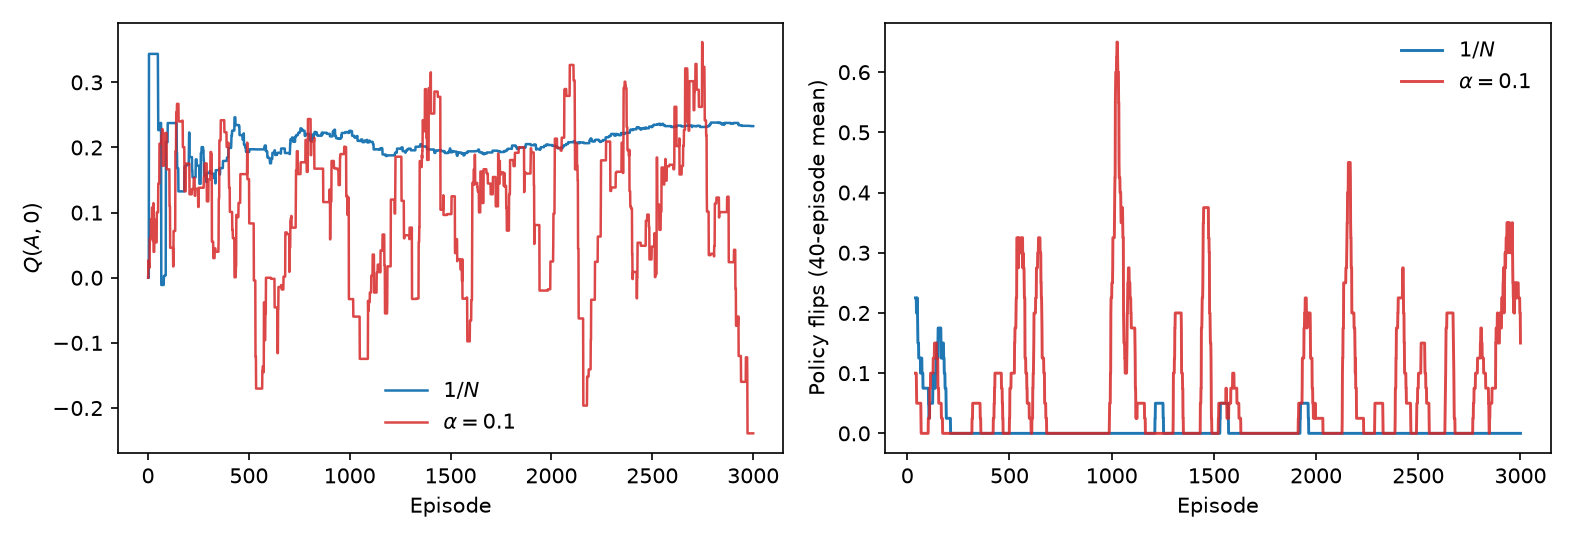
\includegraphics[width=\textwidth]{mc_es_step_size.png}
\caption{Monte Carlo ES, $1/N$ versus $\alpha=0.1$. Left: $Q(A,0)$. Right: greedy-action flips (40-episode mean).}
\label{fig-4-1}
\end{figure}

A bare skeleton is:

\begin{implnote}[Algorithm (Monte Carlo control skeleton)]
Input: none (episodes generated under the current $\pi$).

Output: $Q$ and $\pi$.

\begin{enumerate}
\item Initialize $\pi$ arbitrarily. Initialize $Q(s,a)$ arbitrarily and $N(s,a)\leftarrow 0$.
\item \textbf{Evaluate.} Generate episodes by following the current $\pi$. Update $Q$ by first- or every-visit Monte Carlo averaging of returns (until $Q$ has settled for this $\pi$, or after each episode).
\item \textbf{Improve.} For each $s$, set $\pi(s)\leftarrow\arg\max_a Q(s,a)$.
\item If $\pi$ changed, go to step 2. Otherwise return $Q$ and $\pi$.
\end{enumerate}

\end{implnote}

The skeleton has a problem in Evaluate. Episodes follow the current $\pi$, so $Q$ is updated only for actions $\pi$ actually takes. After Improve, $\pi$ is greedy on $Q$: at each state it picks the single action $\pi(s)=\arg\max_a Q(s,a)$. The next Evaluate then follows that greedy $\pi$ again---so other actions are never tried, their $Q$ entries never improve, and Improve cannot switch to them. The loop can get stuck on a poor policy even though a better action exists.

To get every action tried often enough, change how episodes are generated---and, if needed, how Improve updates $\pi$. This can be done with \textbf{on-policy} or \textbf{off-policy} methods. An on-policy method evaluates and improves the \textbf{same} policy that generates the decisions (and thus the episodes). An off-policy method learns about one policy (the \textbf{target}) while generating data with a different exploring policy (the \textbf{behavior}). Three standard Monte Carlo methods are exploring starts, $\varepsilon$-greedy policies, and off-policy Monte Carlo. The first two are on-policy; the third is off-policy.

\subsection{Exploring starts}

In the skeleton, Improve sets $\pi(s)=\arg\max_a Q(s,a)$, so Evaluate always starts with the same action at $S_0$: $A_0=\pi(S_0)$. Exploring starts replace that first choice by drawing $(S_0,A_0)$ from a distribution that puts positive probability on every pair (e.g. uniform), \textbf{not} from $\pi$; then follow $\pi$ from $S_1$ onward and update $Q$ as usual. That draw is not possible if every episode must begin at a fixed $S_0$ with $A_0=\pi(S_0)$. Improve stays greedy as in the skeleton: $\pi(s)\leftarrow\arg\max_a Q(s,a)$. From $S_1$ the episode follows that $\pi$, so Evaluate and Improve are on the same policy that generates those later actions, and the method is on-policy.
\begin{implnote}[Algorithm (Monte Carlo ES)]
Input: start distribution over $(s,a)$ with positive probability on every pair.

Output: $Q\approx Q^*$ and $\pi\approx\pi^*$.

\begin{enumerate}
\item Initialize $Q(s,a)$ arbitrarily, $N(s,a)\leftarrow 0$, and $\pi$ arbitrarily (e.g. random or greedy on $Q$).
\item Loop forever (each episode):
\begin{itemize}
\item Draw $(S_0,A_0)$ from a distribution over $\mathcal{S}\times\mathcal{A}$ that puts positive probability on every pair (e.g. uniform).
\item Generate the rest of the episode by following $\pi$: $S_0,A_0,R_1,\ldots,S_{T-1},A_{T-1},R_T$.
\item $G\leftarrow 0$. For $t=T{-}1,\ldots,0$:
\begin{itemize}
\item $G\leftarrow R_{t+1}+\gamma G$.
\item If $(S_t,A_t)$ is a first visit in this episode:
\begin{itemize}
\item $N(S_t,A_t)\leftarrow N(S_t,A_t)+1$,
\item $Q(S_t,A_t)\leftarrow Q(S_t,A_t)+\frac{1}{N(S_t,A_t)}\bigl(G-Q(S_t,A_t)\bigr)$.
\end{itemize}
\end{itemize}
\item For each $s$ appearing in the episode: $\pi(s)\leftarrow\arg\max_a Q(s,a)$.
\end{itemize}
\item After enough episodes (or when $\pi$ stops changing), return $Q$ and $\pi$ ($\approx Q^*$, $\approx\pi^*$).
\end{enumerate}

\end{implnote}

The environment of Section 4.2 is reused here. Exploring starts needs its own episode generator:

\lstinputlisting{../code/ch04/mc_es.py}


\subsection{$\varepsilon$-greedy policies}

Another way to try every action is to select with probability instead of always taking the greedy action. Unlike exploring starts, $A_0$ and the following actions are chosen by $\pi$. The greedy action in $Q$ is $A^*=\arg\max_a Q(s,a)$. If Improve set $\pi(s)=A^*$ as in exploring starts, that action would be locked. Therefore, instead of $\pi(s)=A^*$, Improve changes $\pi$ so that $A^*$ is taken with probability $1-\varepsilon$ and otherwise (probability $\varepsilon$) an action is chosen uniformly from $\mathcal{A}$ (the greedy action could also be picked). That selection rule is the policy $\pi$. Evaluate generates every $A_t$ from that same $\pi$. Because we act and learn with the same $\varepsilon$-greedy $\pi$, this is on-policy. The loop aims at the best such exploring policy; driving $\varepsilon\to 0$ carefully recovers a near-greedy optimum. This is the usual practical default.
\begin{implnote}[Algorithm (on-policy first-visit MC control, $\varepsilon$-greedy)]
Input: $\varepsilon\in(0,1]$.

Output: $Q\approx Q^*$ and greedy $\pi\approx\pi^*$ (for acting); learning uses an $\varepsilon$-greedy behavior.

\begin{enumerate}
\item Initialize $Q(s,a)$ arbitrarily, $N(s,a)\leftarrow 0$, and behavior $\pi$ as an arbitrary $\varepsilon$-greedy policy.
\item Loop forever (each episode):
\begin{itemize}
\item Generate an episode by following $\pi$: $S_0,A_0,R_1,\ldots,R_T$.
\item $G\leftarrow 0$. For $t=T{-}1,\ldots,0$:
\begin{itemize}
\item $G\leftarrow R_{t+1}+\gamma G$.
\item If $(S_t,A_t)$ is a first visit in this episode:
\begin{itemize}
\item $N(S_t,A_t)\leftarrow N(S_t,A_t)+1$,
\item $Q(S_t,A_t)\leftarrow Q(S_t,A_t)+\frac{1}{N(S_t,A_t)}\bigl(G-Q(S_t,A_t)\bigr)$.
\end{itemize}
\end{itemize}
\item For each $s$ appearing in the episode:
\begin{itemize}
\item $A^*\leftarrow\arg\max_a Q(s,a)$,
\item set $\pi(\,\cdot\mid s)$ $\varepsilon$-greedy on $A^*$: probability $1-\varepsilon+\varepsilon/|\mathcal{A}|$ on $A^*$, and $\varepsilon/|\mathcal{A}|$ on every other action.
\end{itemize}
\end{itemize}
\item After enough episodes, return $Q$ and the greedy policy $\pi'(s)=\arg\max_a Q(s,a)$ as the estimate of $\pi^*$ (keep $\varepsilon$-greedy $\pi$ only while learning).
\end{enumerate}

\end{implnote}

The environment of Section 4.2 is reused here, and \texttt{greedy\_pi} from Section 4.3. On-policy $\varepsilon$-greedy control is:

\lstinputlisting{../code/ch04/on_policy_mc_control.py}


\subsection{Off-policy Monte Carlo}

In the methods above, the same policy both \textbf{acts} and is \textbf{evaluated}. Off-policy learning splits that role. A \textbf{behavior} policy $b$ generates the episodes (and must keep exploring, e.g. $\varepsilon$-greedy). A \textbf{target} policy $\pi$ is the policy whose action-values we estimate. In this section that $\pi$ is greedy on $Q$: $\pi(s)=\arg\max_a Q(s,a)$. The question is how to estimate $Q^\pi$ when every sample comes from $b$. \textbf{Importance sampling} does that: it estimates an expectation under a target distribution $p$ from samples drawn from a \textbf{proposal} distribution $q$, by reweighting each sample with $p/q$.

The idea of importance sampling (derived in \appref{A}) is to rewrite an expectation under a target distribution $p$ using samples from a proposal distribution $q$:

\[
\mathbb{E}_{x\sim p}[f(x)]
=
\mathbb{E}_{x\sim q}\bigl[w(x)\, f(x)\bigr],
\qquad
w(x)=\frac{p(x)}{q(x)}.
\]

Two forms approximate that expectation from draws $x_i\sim q$---\textbf{ordinary} and \textbf{weighted} importance sampling (see \appref{A}):

\[
\mathbb{E}_{x\sim p}[f(x)]
\approx
\frac{1}{N}\sum_{i=1}^{N} w(x_i)\, f(x_i),
\]

\[
\mathbb{E}_{x\sim p}[f(x)]
\approx
\frac{\sum_{i=1}^{N} w(x_i)\, f(x_i)}{\sum_{i=1}^{N} w(x_i)}.
\]

Here each sample $x$ will be a \textbf{trajectory}; $N$ is the number of such trajectory samples.

For action-values under the target policy,

\begin{equation}
Q^\pi(s,a)
=
\mathbb{E}_\pi[G_t\mid S_t=s,A_t=a].
\tag{4.8}
\end{equation}

An episode generated by the behavior $b$ always starts at $t=0$:

\[
S_0,A_0,R_1,S_1,\ldots,S_{T-1},A_{T-1},R_T.
\]

A trajectory from time $t$, given $S_t$, is

\[
A_t,R_{t+1},S_{t+1},A_{t+1},R_{t+2},\ldots,A_{T-1},R_T.
\]

This is the sample $x$ in the importance-sampling formulas above. The same episode can contain the pair $(S_t,A_t)=(s,a)$ more than once; each occurrence starts its own trajectory sample. The return

\[
G_t=R_{t+1}+\gamma R_{t+2}+\cdots+\gamma^{T-t-1}R_T
\]

is a function of this trajectory ($f(x)=G_t$). Under a policy $\pi$, the probability of the trajectory given $S_t$ is (chain rule; environment factors written as $P(s',r\mid s,a)$)

\[
\begin{aligned}
&P_\pi(A_t,R_{t+1},S_{t+1},\ldots,R_T\mid S_t)
\\
&\quad=
\prod_{k=t}^{T-1}
\pi(A_k\mid S_k)\,
P(S_{k+1},R_{k+1}\mid S_k,A_k).
\end{aligned}
\]

The same expansion under $b$ replaces each $\pi$ by $b$. The importance-sampling weight from the opening of this subsection is their ratio (require $b(a\mid s)>0$ whenever $\pi(a\mid s)>0$):

\begin{equation}
w
=
\rho_{t:T-1}
:=
\frac{P_\pi(A_t,R_{t+1},S_{t+1},\ldots,R_T\mid S_t)}{P_b(A_t,R_{t+1},S_{t+1},\ldots,R_T\mid S_t)}.
\tag{4.9}
\end{equation}

Those environment factors do not depend on the policy: the same $P(S_{k+1},R_{k+1}\mid S_k,A_k)$ appears in $P_\pi$ and in $P_b$. They cancel, so

\[
\rho_{t:T-1}
=
\prod_{k=t}^{T-1}
\frac{\pi(A_k\mid S_k)}{b(A_k\mid S_k)}.
\]

Apply importance sampling \eqref{eq:A.13} to (4.8): the target is $\pi$, the proposal is $b$, the weight is (4.9), and $f=G_t$. Then

\begin{equation}
Q^\pi(s,a)
=
\mathbb{E}_b\bigl[\rho_{t:T-1}\,G_t\mid S_t=s,A_t=a\bigr].
\tag{4.10}
\end{equation}

With $N$ trajectory samples from visits to $(s,a)$ under $b$---each sample $x_i$ the trajectory from that visit, with return $G^{(i)}$ and weight $\rho^{(i)}=\rho_{t:T-1}^{(i)}$---ordinary and weighted importance sampling give

\begin{equation}
Q(s,a)
\approx
\frac{1}{N}\sum_{i=1}^{N}\rho^{(i)}G^{(i)},
\tag{4.11}
\end{equation}

\begin{equation}
Q(s,a)
\approx
\frac{\sum_{i=1}^{N}\rho^{(i)}G^{(i)}}{\sum_{i=1}^{N}\rho^{(i)}}.
\tag{4.12}
\end{equation}

Write $Q_N(s,a)$ for the weighted estimate (4.12). When visit $N{+}1$ brings $G^{(N+1)}(s,a)$ and $\rho^{(N+1)}(s,a)$,

\begin{equation}
Q_{N+1}(s,a)
=
Q_N(s,a)
+
\frac{\rho^{(N+1)}}{\sum_{i=1}^{N+1} \rho^{(i)}}
\Bigl(
G^{(N+1)}(s,a) - Q_N(s,a)
\Bigr).
\tag{4.13}
\end{equation}

To apply (4.13) episode by episode, walk each episode \textbf{backward} ($t=T{-}1,\ldots,0$), as in Section 4.2. Start from $G\leftarrow 0$ and $\rho\leftarrow 1$: that is $G_T=0$ (no rewards after termination) and $\rho_{T:T-1}=1$ (empty product).

At each $t$ while $\rho\neq 0$: form $G_t$ by $G\leftarrow R_{t+1}+\gamma G$, apply (4.13) with the current $\rho$ ($C(s,a)$ stores $\sum_i\rho^{(i)}$), set $\pi(S_t)\leftarrow\arg\max_a Q(S_t,a)$, then $\rho\leftarrow\rho\cdot\pi(A_t\mid S_t)/b(A_t\mid S_t)$. Here $\pi$ is deterministic: it puts probability $1$ on its chosen action at $S_t$ and $0$ on every other action. So if behavior selected $A_t$, then $\pi(A_t\mid S_t)=1$ only when that $A_t$ is $\pi$'s action, and $0$ otherwise. When that factor is $0$, $\rho$ becomes $0$ and the loop stops---further multiplications for earlier times $t{-}1,t{-}2,\ldots$ would leave $\rho$ at $0$.

The behavior $b$ may be any policy. The only requirement is coverage of $\pi$: $b(a\mid s)>0$ whenever $\pi(a\mid s)>0$. Soft or $\varepsilon$-greedy policies always guarantee that, so the denominator of $\rho$ stays positive and a zero $\rho$ comes only from $\pi(A_t\mid S_t)$.

\begin{implnote}[Algorithm (off-policy MC control, weighted importance sampling)]
Input: behavior $b$ with coverage for $\pi$ (e.g. $\varepsilon$-greedy on $Q$).

Output: $Q\approx Q^*$ and greedy $\pi\approx\pi^*$.

\begin{enumerate}
\item Initialize $Q(s,a)$ arbitrarily and $C(s,a)\leftarrow 0$.
\item Loop forever (each episode):
\begin{itemize}
\item $b\leftarrow$ any policy with coverage for $\pi$: $b(a\mid s)>0$ whenever $\pi(a\mid s)>0$ (soft or $\varepsilon$-greedy $b$ always guarantees coverage).
\item Generate an episode by following $b$: $S_0,A_0,R_1,\ldots,S_{T-1},A_{T-1},R_T$.
\item $G\leftarrow 0$, $\rho\leftarrow 1$.
\item For $t=T{-}1,\ldots,0$ while $\rho\neq 0$:
\begin{itemize}
\item $G\leftarrow R_{t+1}+\gamma G$.
\item $C(S_t,A_t)\leftarrow C(S_t,A_t)+\rho$,
\item $Q(S_t,A_t)\leftarrow Q(S_t,A_t)+\frac{\rho}{C(S_t,A_t)}\bigl(G-Q(S_t,A_t)\bigr)$.
\item $\pi(S_t)\leftarrow\arg\max_a Q(S_t,a)$.
\item $\rho\leftarrow\rho\cdot\frac{\pi(A_t\mid S_t)}{b(A_t\mid S_t)}$ ($\pi$ puts probability $1$ on its action at $S_t$ and $0$ on all others; so $\pi(A_t\mid S_t)=1$ if behavior's $A_t$ is that action, else $0$).
\end{itemize}
\end{itemize}
\item After enough episodes, return $Q$ and the greedy $\pi(s)=\arg\max_a Q(s,a)$ ($\approx Q^*$, $\approx\pi^*$).
\end{enumerate}

\end{implnote}

The environment of Section 4.2 is reused here, and \texttt{eps\_greedy} and \texttt{generate\_episode} from Section 4.4.2. Off-policy control is:

\lstinputlisting{../code/ch04/off_policy_mc_control.py}


\subsubsection*{Off-policy state-values}

The same importance-sampling argument gives state-values. With $V^\pi(s)=\mathbb{E}_\pi[G_t\mid S_t=s]$ and the same weight (4.9),

\begin{equation}
V^\pi(s)
=
\mathbb{E}_b\bigl[\rho_{t:T-1}\,G_t\mid S_t=s\bigr].
\tag{4.14}
\end{equation}

With $N$ trajectory samples from visits to $s$ under $b$, returns $G^{(i)}$, and weights $\rho^{(i)}=\rho_{t:T-1}^{(i)}$, ordinary and weighted importance sampling give

\begin{equation}
V(s)
\approx
\frac{1}{N}\sum_{i=1}^{N}\rho^{(i)}G^{(i)},
\tag{4.15}
\end{equation}

\begin{equation}
V(s)
\approx
\frac{\sum_{i=1}^{N}\rho^{(i)}G^{(i)}}{\sum_{i=1}^{N}\rho^{(i)}}.
\tag{4.16}
\end{equation}

Write $V_N(s)$ for the weighted estimate (4.16). When visit $N{+}1$ brings $G^{(N+1)}(s)$ and $\rho^{(N+1)}(s)$,

\begin{equation}
V_{N+1}(s)
=
V_N(s)
+
\frac{\rho^{(N+1)}}{\sum_{i=1}^{N+1} \rho^{(i)}}
\Bigl(
G^{(N+1)}(s) - V_N(s)
\Bigr).
\tag{4.17}
\end{equation}

\chapter{Temporal-Difference Learning}

Chapters 3 and 4 already give two ways to compute values. Neither is ideal in every setting. Dynamic Programming needs the model $P$ and a full backup over every next pair $(s',r)$; Monte Carlo needs no model and uses episode returns $G_t$. Temporal-Difference (TD) learning (\citetxt{sutton1988}{Sutton, 1988}) sits between them: it keeps Monte Carlo's model-free samples and Dynamic Programming's bootstrapping, so the table can be updated from one observed pair $(R_{t+1},S_{t+1})$ rather than waiting for $G_t$. The algorithms below evaluate a given $\pi$ and return $V\approx V^\pi$. They do not replace $\pi$: that Improve step was Section 4.4 for Monte Carlo, and is Chapter 6 for TD.

Those DP limitations follow from the backup: it is a sum over $P$. In Dynamic Programming (Chapter 3), the model $P(s',r\mid s,a)$ is known, so each update is a full backup. Value iteration and the improve step of policy iteration use

\[
V(s)
\leftarrow
\max_a
\sum_{s',r}
P(s',r\mid s,a)\bigl[r+\gamma V(s')\bigr],
\]

while policy evaluation uses the same sum with the fixed action $a=\pi(s)$:

\[
V(s)
\leftarrow
\sum_{s',r}
P(s',r\mid s,\pi(s))\bigl[r+\gamma V(s')\bigr].
\]

Every backup averages over all next pairs $(s',r)$ under $P$, and replaces the rest of the return by the current table entry $V(s')$---that reuse of $V$ is \textbf{bootstrapping}. No episodes are required, only sweeps over the state table. The price is dependence on $P$: if the model is unknown or the sum is infeasible, DP cannot run.

When $P$ is unavailable, Monte Carlo (Chapter 4) generates episodes under $\pi$ and never uses $P$. The return obeys (1.10), $G_t=R_{t+1}+\gamma G_{t+1}$, so $V^\pi(s)=\mathbb{E}_\pi[G_t\mid S_t=s]=\mathbb{E}_\pi[R_{t+1}+\gamma G_{t+1}\mid S_t=s]$. The average of returns from visits to $s$ is

\[
V^\pi(s)
\approx
\frac{1}{N}\sum_{i=1}^{N} G^{(i)}(s),
\]

and the next return is folded in with step-size $\alpha$ as in (4.3)---the \textbf{Monte Carlo} update

\[
V(S_t)
\leftarrow
V(S_t)+\alpha\bigl(G_t-V(S_t)\bigr).
\]

(Here $\alpha=1/(N{+}1)$ recovers an exact sample mean after $N$ prior samples for that state.) Because $G_t$ is built only from observed rewards, there is no sum over $P$ and no lookup of $V(S_{t+1})$. Two difficulties remain. First, $G_t$ stacks many random rewards, so the return from a given state has high variance across visits. Second, $G_t$ is known only when the episode ends, so updates wait for termination: long episodes delay learning, and continuing tasks do not fit.

Both difficulties come from using the full return as the learning target. Equivalently, the same $V^\pi$ takes the compact form, which replaces $G_{t+1}$ by $V^\pi(S_{t+1})$ (\eqref{eq:B.11} in \appref{B}):

\begin{equation}
V^\pi(s)
=
\mathbb{E}_\pi\bigl[R_{t+1}+\gamma V^\pi(S_{t+1})\mid S_t=s\bigr].
\tag{5.1}
\end{equation}

Run the same sample-mean steps as for Monte Carlo---average the one-step backup over visits, then step with $\alpha$---but replace the unknown $V^\pi(S_{t+1})$ by the current table $V(S_{t+1})$. The result is the \textbf{TD} update

\begin{equation}
V(S_t) \leftarrow V(S_t) + \alpha \left[ R_{t+1} + \gamma V(S_{t+1}) - V(S_t) \right]
\tag{5.2}
\end{equation}

Like Monte Carlo, (5.2) needs no $P$: the pair $(R_{t+1},S_{t+1})$ is observed from interaction. Like Dynamic Programming, it bootstraps with a table lookup at the next state. Replacing $G_{t+1}$ by $V(S_{t+1})$ avoids waiting for the episode to end and avoids the high-variance full return $G_t$. The backup $R_{t+1}+\gamma V(S_{t+1})$ still varies across visits, because $R_{t+1}$ and $S_{t+1}$ are random and $V$ is not $V^\pi$. Section 5.1 develops this \textbf{one-step TD} method (TD error and algorithm); Sections 5.2--5.3 extend it to $n$-step TD and TD($\lambda$). Control---$Q$ and an improving $\pi$---is Chapter 6.

\section{One-step TD (TD(0))}

The update (5.2) steps $V(S_t)$ toward the backup $R_{t+1}+\gamma V(S_{t+1})$. That backup uses only the next reward and the table at $S_{t+1}$---a \textbf{one-step} backup. The difference between that backup and the prediction is the \textbf{TD error}---the signal that tells whether $V(S_t)$ should rise or fall:

\begin{equation}
\delta_t
=
\bigl(R_{t+1}+\gamma V(S_{t+1})\bigr) - V(S_t).
\tag{5.3}
\end{equation}

Equivalently, (5.2) is

\[
V(S_t)
\leftarrow
V(S_t)+\alpha\,\delta_t.
\]

If $\delta_t>0$, then $R_{t+1}+\gamma V(S_{t+1})>V(S_t)$, so $V(S_t)$ increases; if $\delta_t<0$, it decreases. That push and pull of $V$ by $\delta_t$ is the learning rule. The lookup $V(S_{t+1})$ in the backup is the bootstrap; $V(S_t)$ is only the prediction being corrected. Both come from the table, so $V$ must be initialized before the first step (an arbitrary table; a common choice is $V\equiv 0$). If $S_{t+1}$ is terminal, take $V(S_{t+1})=0$ and the backup is just $R_{t+1}$.

The step in (5.2) is not the Monte Carlo $1/n$ of \appref{D}. That derivation averages $G$; with $\pi$ and $P$ fixed, $\mathbb{E}[G]=V^\pi$ does not depend on the table. Here the target is $R_{t+1}+\gamma V(S_{t+1})$, which moves with $V$ even when $\pi$ does not. Early backups use a poor $V$; later backups use a better $V$. A $1/n$ weight would fall on the early backups. A constant $\alpha\in(0,1]$ keeps weight on later backups as $V$ improves, and is the usual practical choice.

Unlike Monte Carlo, TD does \textbf{not} generate a full episode and then update. The outer loop starts another episode; the inner loop generates that episode under $\pi$ and applies (5.2) to each observed pair $(R_{t+1},S_{t+1})$. That one-step method is also called \textbf{TD(0)} (the name is explained in Section 5.3):

\begin{implnote}[Algorithm (one-step TD prediction, TD(0))]
Input: policy $\pi$ to evaluate.

Output: estimate $V\approx V^\pi$.

\begin{enumerate}
\item Initialize $V(s)$ arbitrarily (e.g. $0$), with $V(\text{terminal})=0$.
\item Loop for each episode:
\begin{itemize}
\item Initialize $S_0$.
\item For $t=0,1,2,\ldots$ until termination:
\begin{itemize}
\item Take $A_t\sim\pi(\cdot\mid S_t)$, observe $R_{t+1}$, $S_{t+1}$.
\item $V(S_t)\leftarrow V(S_t)+\alpha\bigl[R_{t+1}+\gamma V(S_{t+1})-V(S_t)\bigr]$.
\item $S_t\leftarrow S_{t+1}$.
\end{itemize}
\end{itemize}
\item After enough episodes, return $V$ ($\approx V^\pi$).
\end{enumerate}

\end{implnote}

\lstinputlisting{../code/ch05/td_prediction.py}


\section{$n$-step TD}

TD(0) steps toward one reward and then the table at the next state. A reward that arrives several steps later can change $V(S_t)$ only by passing through those later table entries, and if $V$ is still wrong those entries pollute the backup. $n$-step TD waits for the next $n$ rewards and bootstraps only at $S_{t+n}$, so those rewards enter the target directly. The case $n=1$ is TD(0); waiting until termination recovers the Monte Carlo return $G$. Larger $n$ uses more observed rewards and less of $V$, so less bootstrap error and faster credit, but more variance and a delay of $n$ steps. Intermediate $n$ is often better than either extreme.

The one-step backup already in (5.2) is

\[
U_t^{(1)}=R_{t+1}+\gamma V(S_{t+1}).
\]

Two rewards and a bootstrap at $S_{t+2}$ start from the return identity (1.10), $G_t=R_{t+1}+\gamma G_{t+1}$. Substitute $G_{t+1}=R_{t+2}+\gamma G_{t+2}$:

\begin{equation}
G_t=R_{t+1}+\gamma R_{t+2}+\gamma^2 G_{t+2}.
\tag{5.5}
\end{equation}

$V^\pi(s)=\mathbb{E}_\pi[G_t\mid S_t=s]$. Take that expectation on (5.5) and replace $G_{t+2}$ by $V^\pi(S_{t+2})$ (tower property, as in (5.1)):

\[
V^\pi(s)
=
\mathbb{E}_\pi\bigl[R_{t+1}+\gamma R_{t+2}+\gamma^2 V^\pi(S_{t+2})\mid S_t=s\bigr].
\]

One sample $(R_{t+1},R_{t+2},S_{t+2})$ with the table $V$ in place of $V^\pi$ is the two-step backup (write $U$ for a backup; $G$ stays the true return)

\[
U_t^{(2)}=R_{t+1}+\gamma R_{t+2}+\gamma^2 V(S_{t+2}).
\]

When $V=V^\pi$, $\mathbb{E}_\pi[U_t^{(2)}\mid S_t=s]=V^\pi(s)$. The update is (5.2) with this target:

\[
V(S_t)\leftarrow V(S_t)+\alpha\bigl(U_t^{(2)}-V(S_t)\bigr).
\]

The same pattern with $n$ rewards and a bootstrap at $S_{t+n}$ is

\[
U_t^{(n)}=R_{t+1}+\gamma R_{t+2}+\cdots+\gamma^{n-1}R_{t+n}+\gamma^n V(S_{t+n}),
\]

\[
V(S_t)\leftarrow V(S_t)+\alpha\bigl(U_t^{(n)}-V(S_t)\bigr).
\]

For $n=1$, $U_t^{(1)}$ is the backup in (5.2). If the episode ends at or before $t+n$, then $V(\text{terminal})=0$ and $U_t^{(n)}$ is the remaining return $G_t$. $U_t^{(n)}$ contains $V$, so a constant $\alpha$ is the same practical choice as in Section 5.1.

The method that uses a fixed $n$ is \textbf{$n$-step TD}. It needs the next $n$ transitions (or termination), so an episode is generated first, then $V$ is updated with $U_t^{(n)}$ from a frozen table.

\begin{implnote}[Algorithm ($n$-step TD prediction)]
Input: policy $\pi$ to evaluate; horizon $n\ge 1$.

Output: estimate $V\approx V^\pi$.

\begin{enumerate}
\item Initialize $V(s)$ arbitrarily (e.g. $0$), with $V(\text{terminal})=0$.
\item Loop for each episode:
\begin{itemize}
\item Generate an episode following $\pi$:   $S_0,A_0,R_1,\;\ldots,\;S_{T-1},A_{T-1},R_T$.
\item For each $t=0,1,\ldots,T{-}1$, compute $U_t^{(n)}$ (same frozen table $V$ for every $t$).
\item For each $t=0,1,\ldots,T{-}1$:   $V(S_t)\leftarrow V(S_t)+\alpha\bigl(U_t^{(n)}-V(S_t)\bigr)$.
\end{itemize}
\item After enough episodes, return $V$ ($\approx V^\pi$).
\end{enumerate}

\end{implnote}

\lstinputlisting{../code/ch05/n_step_td_prediction.py}


Section 5.3 mixes several horizons $n$ into one backup and obtains \textbf{TD($\lambda$)}.

\section{TD($\lambda$)}

\textbf{Mixing backups.} In Section 5.2 the learner must pick one fixed horizon $n$: use only $U_t^{(n)}$. That commits to a single tradeoff (short $n$ bootstraps early; long $n$ waits for more rewards). A single horizon is not required. One can instead form \textbf{one} backup by averaging several horizons, then step $V$ toward that mix as in (4.3). For example, give equal weight to the 1-step, 2-step, and 3-step backups:

\[
U
=
\frac{1}{3}U_t^{(1)}+\frac{1}{3}U_t^{(2)}+\frac{1}{3}U_t^{(3)}
=
\sum_{n=1}^{3}\frac{1}{3}\,U_t^{(n)}.
\]

Then

\[
V(S_t)\leftarrow V(S_t)+\alpha\bigl(U-V(S_t)\bigr)
=
V(S_t)+\alpha\Biggl(\sum_{n=1}^{3}\frac{1}{3}\,U_t^{(n)}-V(S_t)\Biggr).
\]

More generally, pick any nonnegative weights $w_n$ that sum to one ($\sum_n w_n=1$) and set

\[
U=\sum_{n} w_n\,U_t^{(n)}.
\]

The equal mix above is the special case $w_1=w_2=w_3=1/3$. The update is again

\[
V(S_t)\leftarrow V(S_t)+\alpha\Biggl(\sum_{n} w_n\,U_t^{(n)}-V(S_t)\Biggr).
\]

The weights must sum to $1$ so $U$ stays a weighted \textbf{average} on the scale of a return (and of $V$). Uniform $w_n=1/N$ is fine for a \textbf{finite} list $n=1,\ldots,N$. It does \textbf{not} extend to $N\to\infty$: you cannot give every $n=1,2,3,\ldots$ the same positive weight and still have $\sum_{n=1}^{\infty} w_n=1$. A flat $1/N$ also gives the same importance to a short backup (few rewards, early use of $V$) and a long backup (many random rewards). Usually one wants short horizons to count more, and long horizons less---that leads to the geometric weights next.

\textbf{Geometric weights and $\lambda$.} Let each longer backup get a fixed fraction $\lambda\in[0,1)$ of the previous weight. The unnormalized weights are $1,\lambda,\lambda^2,\ldots$, i.e. $\lambda^{n-1}$. The first $N$ sum to

\[
1+\lambda+\cdots+\lambda^{N-1}=\frac{1-\lambda^N}{1-\lambda}\qquad(\lambda\neq 1).
\]

If $N\to\infty$ and $\lambda<1$, then $\lambda^N\to 0$, so the infinite sum is $1/(1-\lambda)$. Normalizing gives

\[
w_n=(1-\lambda)\,\lambda^{n-1}.
\]

As $n$ grows, $\lambda^{n-1}$ shrinks ($\lambda<1$), so $w_n$ shrinks. A short backup $U_t^{(1)}$ (one reward, then $V$) has the largest weight; a long backup $U_t^{(n)}$ (many rewards, later $V$) has less. For $\lambda=0.5$: $w_1=1/2$, $w_2=1/4$, $w_3=1/8$, $\ldots$. The resulting mix is the \textbf{$\lambda$-backup}

\begin{equation}
U_t^{\lambda}
=
\sum_{n=1}^{\infty} w_n\,U_t^{(n)}
=
(1-\lambda)\sum_{n=1}^{\infty}\lambda^{n-1}U_t^{(n)},
\tag{5.4}
\end{equation}

and

\[
V(S_t)\leftarrow V(S_t)+\alpha\bigl(U_t^{\lambda}-V(S_t)\bigr).
\]

That method is \textbf{TD($\lambda$)}. At $\lambda=0$, $U_t^{\lambda}=U_t^{(1)}$, which is the one-step backup of Section 5.1 and the $n{=}1$ case of Section 5.2, so that method is named \textbf{TD(0)}. As $\lambda\to 1$, $U_t^{\lambda}\to G_t$ (Monte Carlo)---\textbf{TD(1)}.

\begin{asidenote}[Note]
Equation (5.4) takes $\lambda\in[0,1)$. For every such $\lambda$ the weights still sum to $1$,
\[
\sum_{n=1}^{\infty}(1-\lambda)\lambda^{n-1}=1,
\]
so $U_t^{\lambda}$ is an average, not $0$. Substituting $\lambda=1$ into (5.4) is invalid ($1-\lambda=0$). TD(1) is $\lambda\to 1$ of that average.

Unrolling (1.10) $n$ times (the same pattern as (5.5)) gives
\[
G_t=R_{t+1}+\gamma R_{t+2}+\cdots+\gamma^{n-1}R_{t+n}+\gamma^n G_{t+n}.
\]
Section 5.2 already has
\[
U_t^{(n)}=R_{t+1}+\gamma R_{t+2}+\cdots+\gamma^{n-1}R_{t+n}+\gamma^n V(S_{t+n}).
\]
The first $n$ rewards match, so
\[
U_t^{(n)}-G_t=\gamma^n\bigl(V(S_{t+n})-G_{t+n}\bigr).
\]
$G$ is bounded as in Chapter 1: with $\gamma\in[0,1)$ and bounded rewards, (1.8) converges. $V$ is a finite table, frozen while this backup is formed. With $\alpha\in(0,1]$ the update $V\leftarrow(1-\alpha)V+\alpha U$ is a convex combination; for one-step TD, $U=R+\gamma V(s')$, so if the table already lies in the same interval that bounds $G$, then $U$ stays in that interval and so does $V$. The factor $\gamma^n$ therefore sends the difference to $0$, hence $U_t^{(n)}\to G_t$ as $n\to\infty$. As $\lambda\to 1$, each fixed-$n$ weight vanishes, so the average in (5.4) is carried by large $n$, where $U_t^{(n)}$ is already near $G_t$. Thus $U_t^{\lambda}\to G_t$. The update becomes
\[
V(S_t)\leftarrow V(S_t)+\alpha\bigl(G_t-V(S_t)\bigr),
\]
which is the Monte Carlo step (4.3).
\end{asidenote}

Here $\lambda$ is not a power on $\gamma$ and not the horizon $n$: $n$-step TD (Section 5.2) picks one $U_t^{(n)}$, while $\lambda$ sets how fast the mix forgets longer backups. There is no TD(2) in the $\lambda$ naming. From here on, Section 5.1's method is called TD(0) when contrasting with multi-step or $\lambda$ methods.

On a finite episode that ends at time $T$, the non-terminal states are $S_0,\ldots,S_{T-1}$. From a time $t$ in that episode, Section 5.2's backup $U_t^{(n)}$ uses the next $n$ rewards and then $V(S_{t+n})$. Here $S_{t+n}$ is the state $n$ steps after $S_t$ on the same episode. That state is a non-terminal only while $t+n<T$. If $n\ge T{-}t$, the episode has already ended, so Section 5.2 gives $U_t^{(n)}=G_t$ (the lookup $V(\text{terminal})$ is $0$). The mix (5.4) is unchanged: every term with $n\ge T{-}t$ equals $G_t$. The weights still sum to $1$. The first $T{-}t{-}1$ of them add to $1-\lambda^{T-t-1}$, and the leftover $\lambda^{T-t-1}$ therefore sits on $G_t$:
\begin{equation}
U_t^{\lambda}
=
\sum_{n=1}^{T-t-1}(1-\lambda)\lambda^{n-1}U_t^{(n)}
+
\lambda^{T-t-1}G_t.
\tag{5.6}
\end{equation}
Computing $U_t^{\lambda}$ needs the future rewards of the episode, so the forward-view algorithm below generates an episode first, then updates toward (5.6)---unlike online TD(0).

\begin{implnote}[Algorithm (forward-view TD($\lambda$) prediction)]
Input: policy $\pi$ to evaluate; $\lambda\in[0,1]$.

Output: estimate $V\approx V^\pi$.

\begin{enumerate}
\item Initialize $V(s)$ arbitrarily (e.g. $0$), with $V(\text{terminal})=0$.
\item Loop for each episode:
\begin{itemize}
\item Generate an episode following $\pi$:   $S_0,A_0,R_1,\;S_1,A_1,R_2,\;\ldots,\;S_{T-1},A_{T-1},R_T$.
\item For each $t=0,1,\ldots,T{-}1$, compute $U_t^{\lambda}$ from (5.6) (same frozen table $V$ for every $t$).
\item For each $t=0,1,\ldots,T{-}1$:   $V(S_t)\leftarrow V(S_t)+\alpha\bigl(U_t^{\lambda}-V(S_t)\bigr)$.
\end{itemize}
\item After enough episodes, return $V$ ($\approx V^\pi$).
\end{enumerate}

\end{implnote}

\lstinputlisting{../code/ch05/td_lambda_prediction.py}


\chapter{TD Control: SARSA, Q-Learning, and Exploration}

\textbf{Control} asks which \textit{action} to prefer from the current state, but one-step TD (5.2) only learns how good each \textit{state} is under a fixed policy---a table of $V$ does not score actions. With a known model, DP can still choose the action
\[
\pi(s)=\arg\max_a\sum_{s',r}P(s',r\mid s,a)\bigl[r+\gamma V(s')\bigr];
\]
without that $P$, the sum cannot be computed, so the $V$ table alone cannot rank actions. Model-free control therefore uses action-values $Q(s,a)$, which score each pair, so $\arg\max_a Q(s,a)$ needs no model. Monte Carlo control uses that idea, but learns $Q$ only from full returns $G_t$. This section keeps $Q$ for control and replaces that full-return backup by one-step TD, stepping $Q(S_t,A_t)$ toward a bootstrap from $Q$ at the next state. Two standard algorithms do that---\textbf{SARSA}, which is on-policy (the backup uses the next action the behavior policy actually takes), and \textbf{Q-learning}, which is off-policy (the backup uses a $\max$ over next actions).

\section{SARSA}

The update (5.2) steps $V(S_t)$ toward $R_{t+1}+\gamma V(S_{t+1})$, which cannot choose $\pi(S_t)$ without $P$. Replacing $V(S_t)$ by $Q(S_t,A_t)$ scores the action that was taken, by stepping $Q(S_t,A_t)$ toward $R_{t+1}+\gamma Q(S_{t+1},A_{t+1})$. Drawing both $A_t$ and $A_{t+1}$ from the same behavior $\pi$ makes the table estimate $Q^\pi$---that is \textbf{on-policy}. The method is \textbf{SARSA} (\textbf{S}tate--\textbf{A}ction--\textbf{R}eward--\textbf{S}tate--\textbf{A}ction), named for the five-tuple $(S_t,A_t,R_{t+1},S_{t+1},A_{t+1})$ that the update uses. SARSA was introduced under that name by Sutton (\citetxt{suttonbarto2018}{Sutton and Barto, 2018}); the learning update is a variation of the on-policy backup of \citetxt{rummery1994}{Rummery and Niranjan, 1994}, who studied it with neural function approximation. In this book we use the tabular form: one $Q(s,a)$ entry per pair, updated by (6.3) below.

The values $Q^\pi$ obey the compact Bellman expectation equation, the action-value analogue of (5.1) (\eqref{eq:B.18} in \appref{B}):

\begin{equation}
Q^\pi(s,a)
=
\mathbb{E}_\pi\bigl[R_{t+1}+\gamma Q^\pi(S_{t+1},A_{t+1})\mid S_t=s,A_t=a\bigr].
\tag{6.1}
\end{equation}

Here $A_{t+1}$ is drawn from $\pi$ at $S_{t+1}$. Observe one transition and that next action and, because $Q^\pi$ is unknown, put the current table estimate $Q$ in its place to form the one-step backup

\[
U_t=R_{t+1}+\gamma Q(S_{t+1},A_{t+1}).
\]

(If $S_{t+1}$ is terminal, take the $Q$ term as $0$.) The difference between that backup and the current estimate is the \textbf{TD error} on the pair---the same idea as (5.3):

\begin{equation}
\delta_t
=
\bigl(R_{t+1}+\gamma Q(S_{t+1},A_{t+1})\bigr) - Q(S_t,A_t).
\tag{6.2}
\end{equation}

Stepping $Q(S_t,A_t)$ toward $U_t$ with step-size $\alpha$ is (5.2) on pairs; the expanded and $\delta$ forms are the same update:

\begin{equation}
\begin{aligned}
Q(S_t,A_t)
&\leftarrow
Q(S_t,A_t)
+
\alpha\bigl[R_{t+1}+\gamma Q(S_{t+1},A_{t+1})-Q(S_t,A_t)\bigr]
\\
&=
Q(S_t,A_t)+\alpha\,\delta_t.
\end{aligned}
\tag{6.3}
\end{equation}

Because $A_{t+1}$ is chosen the same way as $A_t$, both from the behavior $\pi$, the actions in the backup match how we act, and the table estimates $Q^\pi$ for that same $\pi$. That is what \textbf{on-policy} means here. Recall that a \textbf{policy} is only the rule for picking an action given the state (Section 1.1), not the $Q$ table itself. Here that rule is $\varepsilon$-greedy in the \textbf{current} $Q$. With probability $1-\varepsilon$ take $\arg\max_a Q(s,a)$, otherwise pick uniformly in $\mathcal{A}$. Step 1 sets $Q(s,a)$ arbitrarily; $S_{t+1}$ comes from the environment after we take $A_t$; then $A_{t+1}$ is sampled from that $\varepsilon$-greedy $\pi$. As $Q$ improves, the same $\varepsilon$-greedy rule (now reading the new $Q$) is the updated behavior. That is evaluate--improve as in Monte Carlo control, but with a one-step TD evaluate step. The algorithm also returns $\pi'(s)=\arg\max_a Q(s,a)$. That $\pi'$ is greedy in the finished $Q$, not the $\varepsilon$-greedy $\pi$ used while learning.

Unlike Monte Carlo, SARSA does not generate the full episode first. Step 2 still loops for each episode, but the whole trajectory is not produced before updating. After $S_0$ and $A_0$, each inner step observes $(R_{t+1},S_{t+1})$, chooses $A_{t+1}$, and applies (6.3). The rest of the episode is generated only after that update, one transition at a time, until termination.

\begin{implnote}[Algorithm (SARSA: on-policy TD control)]
Input: $\varepsilon\in(0,1]$ (exploration); action set $\mathcal{A}$.

Output: $Q\approx Q^\pi$ for the $\varepsilon$-greedy $\pi$ used while learning; greedy $\pi'(s)=\arg\max_a Q(s,a)$.

\begin{enumerate}
\item Initialize $Q(s,a)$ arbitrarily, with $Q(\text{terminal},\,\cdot\,)=0$.
\item Loop for each episode:
\begin{itemize}
\item Initialize $S_0$ (starting state of the episode).
\item Choose $A_0$ from $Q$ $\varepsilon$-greedy in $S_0$ (over $\mathcal{A}$).
\item For $t=0,1,2,\ldots$ until termination:
\begin{itemize}
\item Take $A_t$, observe $R_{t+1}$, $S_{t+1}$.
\item Choose $A_{t+1}$ from $Q$ $\varepsilon$-greedy in $S_{t+1}$.
\item $Q(S_t,A_t)\leftarrow Q(S_t,A_t)+\alpha\bigl[R_{t+1}+\gamma Q(S_{t+1},A_{t+1})-Q(S_t,A_t)\bigr]$.
\end{itemize}
\end{itemize}
\item After enough episodes, return $Q$ and $\pi'(s)=\arg\max_a Q(s,a)$.
\end{enumerate}

\end{implnote}

\lstinputlisting{../code/ch06/sarsa.py}


\section{Q-learning}

The SARSA algorithm above returns $\pi'(s)=\arg\max_a Q(s,a)$. That $\pi'$ is greedy in the finished $Q\approx Q^\pi$; it is not the $\varepsilon$-greedy $\pi$ used while learning. $\pi^*$ is an optimal policy, $\pi^*(s)=\arg\max_a Q^*(s,a)$ (2.11). SARSA's $\pi'$ is not $\pi^*$ unless the exploring $\pi$ was already optimal. A different goal is to learn $Q^*$ so that this greedy $\pi'$ aims at $\pi^*$ while still exploring with behavior. That method is \textbf{Q-learning} (\citetxt{watkins1992}{Watkins and Dayan, 1992}), the same one-step TD pattern on pairs, except the bootstrap uses a $\max$ over next actions instead of the behavior's next action. The update (6.6) below is their tabular rule.

The targets $Q^*$ obey the compact Bellman optimality equation (\eqref{eq:C.5} in \appref{C}):

\begin{equation}
Q^*(s,a)
=
\mathbb{E}\bigl[R_{t+1}+\gamma\max_{a'} Q^*(S_{t+1},a')\mid S_t=s,A_t=a\bigr].
\tag{6.4}
\end{equation}

Unlike (6.1), the continuation after $S_{t+1}$ is a $\max$ over actions, not an action drawn from a behavior $\pi$. Observe one transition and, because $Q^*$ is unknown, put the current table estimate $Q$ in its place to form the one-step backup

\[
U_t=R_{t+1}+\gamma\max_{a'} Q(S_{t+1},a').
\]

(If $S_{t+1}$ is terminal, take the $\max$ term as $0$.) The \textbf{TD error} on the pair is again backup minus estimate:

\begin{equation}
\delta_t
=
\bigl(R_{t+1}+\gamma\max_{a'} Q(S_{t+1},a')\bigr) - Q(S_t,A_t).
\tag{6.5}
\end{equation}

Stepping $Q(S_t,A_t)$ toward $U_t$ is the same $\alpha$-update as (6.3), with this backup:

\begin{equation}
\begin{aligned}
Q(S_t,A_t)
&\leftarrow
Q(S_t,A_t)
+
\alpha\bigl[R_{t+1}+\gamma\max_{a'} Q(S_{t+1},a')-Q(S_t,A_t)\bigr]
\\
&=
Q(S_t,A_t)+\alpha\,\delta_t.
\end{aligned}
\tag{6.6}
\end{equation}

Unlike SARSA, where both the current action $A_t$ and the next action $A_{t+1}$ are chosen by the same behavior policy (e.g. $\varepsilon$-greedy in $Q$), Q-learning does not put a behavior-sampled $A_{t+1}$ in the backup. The next action is whichever $a'$ currently maximizes $Q(S_{t+1},a')$. Acting may still use $\varepsilon$-greedy for $A_t$ to explore; only how the backup treats the next action differs. That is why Q-learning is \textbf{off-policy}. No importance-sampling weights are needed. The $\max$ already puts the greedy target inside the one-step backup.

As in SARSA, the full episode is not generated first. Start at $S_0$, then for each step choose behavior $A_t$, observe $(R_{t+1},S_{t+1})$, and apply (6.6). There is no stored full return.

\begin{implnote}[Algorithm (Q-learning: off-policy TD control)]
Input: $\varepsilon\in(0,1]$ (behavior exploration); action set $\mathcal{A}$.

Output: $Q\approx Q^*$; greedy $\pi(s)=\arg\max_a Q(s,a)$.

\begin{enumerate}
\item Initialize $Q(s,a)$ arbitrarily, with $Q(\text{terminal},\,\cdot\,)=0$.
\item Loop for each episode:
\begin{itemize}
\item Initialize $S_0$ (starting state of the episode).
\item For $t=0,1,2,\ldots$ until termination:
\begin{itemize}
\item Choose $A_t$ from $Q$ $\varepsilon$-greedy in $S_t$ (behavior; over $\mathcal{A}$).
\item Take $A_t$, observe $R_{t+1}$, $S_{t+1}$.
\item $Q(S_t,A_t)\leftarrow Q(S_t,A_t)+\alpha\bigl[R_{t+1}+\gamma\max_{a'} Q(S_{t+1},a')-Q(S_t,A_t)\bigr]$.
\end{itemize}
\end{itemize}
\item After enough episodes, return $Q$ and $\pi(s)=\arg\max_a Q(s,a)$.
\end{enumerate}

\end{implnote}

\lstinputlisting{../code/ch06/q_learning.py}


\section{$\varepsilon$-greedy}

SARSA and Q-learning choose $A_t$ $\varepsilon$-greedy in the current $Q$ (SARSA also chooses $A_{t+1}$ that way). That rule is formulated here in mathematical form as a distribution $\pi(a\mid s)$ over $\mathcal{A}$. It is essentially the same choice as above, only written as (6.7), with an optional schedule (6.8) that shrinks $\varepsilon$. \textbf{Exploit} takes $\arg\max_a Q(s,a)$, so the action uses the current table. \textbf{Explore} draws uniformly from $\mathcal{A}$, so other pairs $(s,a)$ are visited and their $Q$ can update. $Q$ is updated only at the pair that was taken, so both are needed. With probability $1-\varepsilon$ exploit, and with probability $\varepsilon$ explore.

At state $s$, write $A^*=\arg\max_a Q(s,a)$ (break ties by any fixed rule). Because $A^*$ is still eligible on the uniform draw, its total probability is the greedy branch plus one share of that draw,

\[
\pi(A^*\mid s)
=
(1-\varepsilon)
+
\frac{\varepsilon}{\lvert\mathcal{A}\rvert}.
\]

Every other action appears only on the uniform draw, each with probability $\varepsilon/\lvert\mathcal{A}\rvert$. For $\varepsilon\in(0,1]$,

\begin{equation}
\pi(a\mid s)
=
\begin{cases}
1-\varepsilon+\dfrac{\varepsilon}{\lvert\mathcal{A}\rvert},
&
\text{if }a=A^*,
\\[0.75em]
\dfrac{\varepsilon}{\lvert\mathcal{A}\rvert},
&
\text{if }a\neq A^*.
\end{cases}
\tag{6.7}
\end{equation}

When $\varepsilon=0$, (6.7) is greedy. When $\varepsilon=1$, it is uniform. A fixed $\varepsilon>0$ explores forever, which helps coverage but keeps the behavior away from the greedy $\pi^*$. A common remedy is to shrink $\varepsilon$ over episodes $k=0,1,2,\ldots$ by a geometric factor. Writing $\varepsilon_k=\varepsilon_0^k$ does not work when the start is $\varepsilon_0=1$ (then $1^k=1$ forever), and it ties the starting level to the decay speed. Keep them separate: start at $\varepsilon_0\in(0,1]$ and multiply by $\lambda^k$ with $\lambda\in(0,1)$,

\begin{equation}
\varepsilon_k
=
\varepsilon_0\,\lambda^k.
\tag{6.8}
\end{equation}

Early episodes explore more; later ones concentrate on $\arg\max_a Q(s,a)$. In practice one may clip $\varepsilon_k$ below by a small floor so a little exploration remains; that floor is optional and is not part of (6.8). The same schedule can feed any method that chooses $A_t$ by (6.7)---including on-policy MC control, SARSA, and Q-learning.

The algorithm and code below are only that choice piece: given $Q$, $s$, and an $\varepsilon$ (optionally from (6.8)), return one action from (6.7). They are not a full control loop---no environment step, no $Q$ update. Plug \texttt{eps\_greedy} in wherever Chapters 4--6 chose $A_t$ (or SARSA's $A_{t+1}$) $\varepsilon$-greedy; use \texttt{eps\_schedule} when $\varepsilon$ should shrink over episodes.

\begin{implnote}[Algorithm (sample $A\sim\varepsilon$-greedy in $Q$)]
Input: $Q$, state $s$, $\varepsilon\in[0,1]$, action set $\mathcal{A}$.

\begin{enumerate}
\item $A^*\leftarrow\arg\max_a Q(s,a)$.
\item For each $a\in\mathcal{A}$, set $\pi(a\mid s)$ by (6.7): $1-\varepsilon+\varepsilon/\lvert\mathcal{A}\rvert$ if $a=A^*$, else $\varepsilon/\lvert\mathcal{A}\rvert$.
\item Return a draw from $\pi(\cdot\mid s)$.
\end{enumerate}

\end{implnote}

\lstinputlisting{../code/ch06/eps_greedy.py}


\section{Softmax}

$\varepsilon$-greedy in (6.7) uses $Q$ only to pick the greedy action $A^*$. Every other action then shares the same mass $\varepsilon/\lvert\mathcal{A}\rvert$, so a near-best action and a terrible one are treated alike when exploring.

To rank every action by $Q$ instead, use a \textbf{Boltzmann (Gibbs)} distribution over $\mathcal{A}$: $\pi(a\mid s)\propto\exp\bigl(Q(s,a)/\tau\bigr)$, so better actions are more likely and temperature $\tau>0$ sets how sharp the ranking is. \textbf{Softmax} writes that distribution in normalized form---exponentiate each score $Q/\tau$, then divide by the sum:

\begin{equation}
\pi(a\mid s)
=
\frac{\exp\bigl(Q(s,a)/\tau\bigr)}
{\sum_{b\in\mathcal{A}}\exp\bigl(Q(s,b)/\tau\bigr)}.
\tag{6.9}
\end{equation}

Large $\tau$ flattens $\pi$ toward uniform; small $\tau$ concentrates on $\arg\max_a Q(s,a)$. At $\tau=1$, (6.9) is the plain softmax of $Q$. Leave $\tau$ untuned and the sharpness tracks whatever scale $Q$ happens to have, so treat $\tau$ as a hyperparameter---fixed by trying a few values, or annealed over episodes like (6.8).

The algorithm and code below only return one draw from (6.9); they are not a full control loop. Use them in place of $\varepsilon$-greedy when selecting $A_t$ (or SARSA's $A_{t+1}$).

\begin{implnote}[Algorithm (sample $A\sim$ softmax in $Q$)]
Input: $Q$, state $s$, temperature $\tau>0$, action set $\mathcal{A}$.

\begin{enumerate}
\item For each $a\in\mathcal{A}$, set $u(a)\leftarrow\exp\bigl(Q(s,a)/\tau\bigr)$.
\item For each $a\in\mathcal{A}$, set $\pi(a\mid s)\leftarrow u(a)/\sum_{b\in\mathcal{A}} u(b)$ as in (6.9).
\item Return a draw from $\pi(\cdot\mid s)$.
\end{enumerate}

\end{implnote}

\lstinputlisting{../code/ch06/softmax.py}


SARSA, Q-learning, (6.7), and (6.9) all use a table of $Q(s,a)$: one entry per pair, updated only when that pair is taken. That table works because $\mathcal{S}$ so far is a small fixed set. The same $s$ returns, and the same cell is updated. When $\mathcal{S}$ is large or continuous, it runs into two problems: the table does not fit, and a later observed state is almost never that same $s$, so the stored number is not used again. Chapter 7 replaces the table by a function $\hat{Q}(s,a;\mathbf{w})$ of a weight vector $\mathbf{w}$. Only those weights are stored and updated. SARSA and Q-learning keep the same backups, and (6.7) and (6.9) still choose $A_t$, now from $\hat{Q}$.

\chapter{Function Approximation and the Deadly Triad}

Chapters 3--6 stored value in a \textbf{table}, one entry $V(s)$ or $Q(s,a)$ per state or pair, updated only at visited keys. Chapter 6 then specified how to choose $A_t$ from that table ($\varepsilon$-greedy or softmax). Tabular control is fine when $\mathcal{S}$ and $\mathcal{A}$ are small and discrete, as in Chapters 3--6. The same $s$ returns, and the same cell is updated. Many tasks have continuous states, images, or huge discrete spaces. Then a separate number for every $(s,a)$ runs into two problems: the table does not fit in memory, and a later observed state is almost never that same $s$, so the stored number is not used again.

\textbf{Function approximation} addresses both. In the tabular case the object we store is a whole map---either $s\mapsto V(s)$ or $(s,a)\mapsto Q(s,a)$---one free number per key. Replace that map by a function of a weight vector $\mathbf{w}\in\mathbb{R}^d$ with components $w_1,\ldots,w_d$:

\[
\hat{V}(s;\mathbf{w})\approx V(s)
\qquad\text{or}\qquad
\hat{Q}(s,a;\mathbf{w})\approx Q(s,a),
\]

with $d$ much smaller than the number of keys (or finite $d$ even when $\mathcal{S}$ is continuous). Only the $d$ weights are stored and updated. For action-values we use a \textbf{feature map} $\mathbf{x}$: given $(s,a)$, it returns a feature vector $\mathbf{x}(s,a)\in\mathbb{R}^d$ of the same length as $\mathbf{w}$. The map itself is fixed---the same pair always produces the same vector; different pairs may produce different vectors. The linear case in (7.1) is the inner product $\hat{Q}(s,a;\mathbf{w})=\mathbf{w}^\top\mathbf{x}(s,a)$. (State-values use an analogous $\mathbf{x}(s)\in\mathbb{R}^d$ and $\hat{V}(s;\mathbf{w})=\mathbf{w}^\top\mathbf{x}(s)$.) At time $t$ one writes $\mathbf{x}_t=\mathbf{x}(S_t,A_t)$ for that step's feature vector. Changing $\mathbf{w}$ changes the prediction at every input whose features use those weights, so experience at one key transfers to others---that is generalization. The rest of this section and Chapter 8 develop the $Q$ form used for control; the $V$ form is the same idea for prediction. Exploration is unchanged: $\varepsilon$-greedy or softmax still choose $A_t$ from predicted action-values (Chapter 6). What changes is the representation and the update.

This section develops that idea in two steps. First, Section 7.1 lifts tabular control to a linear approximator: off-policy Q-learning FA (7.3) and on-policy SARSA FA (7.4). Function approximation itself is neither on-policy nor off-policy---that label belongs to the update. Second, Section 7.2 discusses the \textbf{deadly triad}, in which off-policy semi-gradient FA can diverge, while on-policy linear FA is known to be stable. Chapter 8 then introduces the practical fixes used in deep Q-learning.

\section{Linear Function Approximation}

As discussed at the start of this section, a separate table entry for every $(s,a)$ is often infeasible, so we represent $Q$ by a function of weights. The linear form is

\begin{equation}
\hat{Q}(s,a;\mathbf{w})
=
\mathbf{w}^\top \mathbf{x}(s,a)
=
\sum_{i=1}^{d} w_i\, x_i(s,a),
\tag{7.1}
\end{equation}

with a fixed feature map $\mathbf{x}(s,a)\in\mathbb{R}^d$. Only $\mathbf{w}$ is learned. Differentiating (7.1) gives

\begin{equation}
\nabla_{\mathbf{w}} \hat{Q}(s,a;\mathbf{w})
=
\mathbf{x}(s,a).
\tag{7.2}
\end{equation}

For state-values the same construction uses features of the state alone, $\hat{V}(s;\mathbf{w})=\mathbf{w}^\top\mathbf{x}(s)$.

We still learn online over episodes. At each time step $t$ of an episode, the agent is at $(S_t,A_t)$, observes a transition, and updates $\mathbf{w}$ once. Write $\mathbf{x}_t=\mathbf{x}(S_t,A_t)$ and $\hat{Q}_t=\hat{Q}(S_t,A_t;\mathbf{w})=\mathbf{w}^\top\mathbf{x}_t$. The TD control updates from Chapter 6 carry over with the table $Q$ replaced by the approximator $\hat{Q}$. \textbf{On-policy} (SARSA) is

\[
\begin{aligned}
\hat{Q}(S_t,A_t;\mathbf{w})
&\leftarrow
\hat{Q}(S_t,A_t;\mathbf{w})
+
\alpha\bigl[R_{t+1}+\gamma\hat{Q}(S_{t+1},A_{t+1};\mathbf{w})-\hat{Q}(S_t,A_t;\mathbf{w})\bigr]
\\
&=
\hat{Q}(S_t,A_t;\mathbf{w})
+
\alpha\bigl(U_t-\hat{Q}(S_t,A_t;\mathbf{w})\bigr),
\end{aligned}
\]

with $U_t=R_{t+1}+\gamma\hat{Q}(S_{t+1},A_{t+1};\mathbf{w})$. \textbf{Off-policy} (Q-learning) is

\[
\begin{aligned}
\hat{Q}(S_t,A_t;\mathbf{w})
&\leftarrow
\hat{Q}(S_t,A_t;\mathbf{w})
+
\alpha\bigl[R_{t+1}+\gamma\max_{a'}\hat{Q}(S_{t+1},a';\mathbf{w})-\hat{Q}(S_t,A_t;\mathbf{w})\bigr]
\\
&=
\hat{Q}(S_t,A_t;\mathbf{w})
+
\alpha\bigl(U_t-\hat{Q}(S_t,A_t;\mathbf{w})\bigr),
\end{aligned}
\]

with $U_t=R_{t+1}+\gamma\max_{a'}\hat{Q}(S_{t+1},a';\mathbf{w})$. (If $S_{t+1}$ is terminal, take the $\gamma$ term as $0$ in either case.) The two methods differ only in that backup $U_t$.

Those displays state the intended change in $\hat{Q}$ at the visited pair. There is no separate table entry to write into: $\hat{Q}$ is determined by $\mathbf{w}$, so the update is realized by changing $\mathbf{w}$. The squared gap to close is the one-step objective

\[
J_t(\mathbf{w})
=
\frac{1}{2}\bigl(U_t-\hat{Q}(S_t,A_t;\mathbf{w})\bigr)^2
=
\frac{1}{2}\bigl(U_t-\mathbf{w}^\top\mathbf{x}_t\bigr)^2.
\]

Because $U_t$ bootstraps $\hat{Q}(\cdot;\mathbf{w})$, it depends on $\mathbf{w}$. The gradient of $J_t$ is

\[
\nabla_{\mathbf{w}} J_t(\mathbf{w})
=
\bigl(U_t-\mathbf{w}^\top\mathbf{x}_t\bigr)
\bigl(\nabla_{\mathbf{w}} U_t-\mathbf{x}_t\bigr).
\]

\textbf{Full-gradient} descent uses that expression as written. \textbf{Semi-gradient} sets $\nabla_{\mathbf{w}} U_t=\mathbf{0}$ when differentiating, then $\mathbf{w}\leftarrow\mathbf{w}+\alpha\bigl(U_t-\mathbf{w}^\top\mathbf{x}_t\bigr)\,\mathbf{x}_t$. How $U_t$ is formed decides on-policy vs off-policy. The next two subsections spell each case out.

\subsection{Q-learning}

Q-learning is \textbf{off-policy} because the $\max$ backup learns about a greedy continuation while behavior may explore (Chapter 6). Take the off-policy $U_t$ from above,

\[
U_t=R_{t+1}+\gamma\max_{a'}\hat{Q}(S_{t+1},a';\mathbf{w}).
\]

For the greedy action $a^*=\arg\max_{a'}\hat{Q}(S_{t+1},a';\mathbf{w})$ (break ties arbitrarily), $U_t=R_{t+1}+\gamma\mathbf{w}^\top\mathbf{x}(S_{t+1},a^*)$ when $S_{t+1}$ is nonterminal. Differentiating and using (7.2) gives $\nabla_{\mathbf{w}} U_t=\gamma\mathbf{x}(S_{t+1},a^*)$ (since $R_{t+1}$ does not depend on $\mathbf{w}$). If $S_{t+1}$ is terminal, $U_t=R_{t+1}$ and $\nabla_{\mathbf{w}} U_t=\mathbf{0}$.

Full-gradient descent on $J_t$ is

\[
\begin{aligned}
\mathbf{w}
&\leftarrow
\mathbf{w}
-
\alpha\,\nabla_{\mathbf{w}} J_t(\mathbf{w})
\\
&=
\mathbf{w}
-
\alpha\,
\bigl(U_t-\mathbf{w}^\top\mathbf{x}_t\bigr)
\bigl(\nabla_{\mathbf{w}} U_t-\mathbf{x}_t\bigr).
\end{aligned}
\]

Semi-gradient sets $\nabla_{\mathbf{w}} U_t=\mathbf{0}$ and yields

\begin{equation}
\mathbf{w}
\leftarrow
\mathbf{w}
+
\alpha
\Bigl[
R_{t+1}
+
\gamma\max_{a'}\bigl(\mathbf{w}^\top\mathbf{x}(S_{t+1},a')\bigr)
-
\mathbf{w}^\top\mathbf{x}_t
\Bigr]
\mathbf{x}_t.
\tag{7.3}
\end{equation}

Equivalently, $\mathbf{w}\leftarrow\mathbf{w}+\alpha\bigl[R_{t+1}+\gamma\max_{a'}\hat{Q}(S_{t+1},a';\mathbf{w})-\hat{Q}(S_t,A_t;\mathbf{w})\bigr]\mathbf{x}(S_t,A_t)$. This keeps the $\max$ backup, so it is off-policy.

Semi-gradient ignores the dependence of $U_t$ on $\mathbf{w}$ when differentiating $J_t$. That does not freeze the target across learning: after $\mathbf{w}$ is updated, the next transition builds a new $U_t$ from the new $\hat{Q}$. So the bootstrap still \textbf{moves} every step.

\begin{implnote}[Algorithm (full-gradient Q-learning with linear FA)]
Input: feature map $\mathbf{x}(s,a)$; step size $\alpha$; discount $\gamma$; exploration (e.g. $\varepsilon$-greedy).

Output: $\mathbf{w}$ such that $\hat{Q}(s,a;\mathbf{w})=\mathbf{w}^\top\mathbf{x}(s,a)\approx Q^*(s,a)$; greedy policy $\pi(s)=\arg\max_a\hat{Q}(s,a;\mathbf{w})$.

\begin{enumerate}
\item Initialize $\mathbf{w}$ arbitrarily (e.g. $\mathbf{0}$).
\item Loop for each episode:
\begin{itemize}
\item Initialize $S$.
\item For each step of the episode until $S$ is terminal:
\begin{itemize}
\item Choose $A$ from $S$ using a policy based on $\hat{Q}(\cdot,\cdot;\mathbf{w})$ (e.g. $\varepsilon$-greedy).
\item Take $A$; observe $R$, $S'$.
\item $\mathbf{x}\leftarrow\mathbf{x}(S,A)$.
\item If $S'$ is terminal:
\begin{itemize}
\item $U\leftarrow R$
\item $\mathbf{g}_U\leftarrow\mathbf{0}$
\end{itemize}
\item Else:
\begin{itemize}
\item $a^*\leftarrow\arg\max_{a'}\mathbf{w}^\top\mathbf{x}(S',a')$
\item $U\leftarrow R+\gamma\mathbf{w}^\top\mathbf{x}(S',a^*)$
\item $\mathbf{g}_U\leftarrow\gamma\mathbf{x}(S',a^*)$
\end{itemize}
\item $\mathbf{w}\leftarrow\mathbf{w}-\alpha\bigl(U-\mathbf{w}^\top\mathbf{x}\bigr)(\mathbf{g}_U-\mathbf{x})$.
\item $S\leftarrow S'$.
\end{itemize}
\end{itemize}
\item Return $\mathbf{w}$ and $\pi(s)=\arg\max_a\hat{Q}(s,a;\mathbf{w})$.
\end{enumerate}

\end{implnote}

\begin{implnote}[Algorithm (semi-gradient Q-learning with linear FA)]
Input: feature map $\mathbf{x}(s,a)$; step size $\alpha$; discount $\gamma$; exploration (e.g. $\varepsilon$-greedy).

Output: $\mathbf{w}$ such that $\hat{Q}(s,a;\mathbf{w})=\mathbf{w}^\top\mathbf{x}(s,a)\approx Q^*(s,a)$; greedy policy $\pi(s)=\arg\max_a\hat{Q}(s,a;\mathbf{w})$.

\begin{enumerate}
\item Initialize $\mathbf{w}$ arbitrarily (e.g. $\mathbf{0}$).
\item Loop for each episode:
\begin{itemize}
\item Initialize $S$.
\item For each step of the episode until $S$ is terminal:
\begin{itemize}
\item Choose $A$ from $S$ using a policy based on $\hat{Q}(\cdot,\cdot;\mathbf{w})$ (e.g. $\varepsilon$-greedy).
\item Take $A$; observe $R$, $S'$.
\item $\mathbf{x}\leftarrow\mathbf{x}(S,A)$.
\item If $S'$ is terminal:
\begin{itemize}
\item $U\leftarrow R$
\end{itemize}
\item Else:
\begin{itemize}
\item $U\leftarrow R+\gamma\max_{a'}\mathbf{w}^\top\mathbf{x}(S',a')$
\end{itemize}
\item $\mathbf{w}\leftarrow\mathbf{w}+\alpha\bigl(U-\mathbf{w}^\top\mathbf{x}\bigr)\,\mathbf{x}$.
\item $S\leftarrow S'$.
\end{itemize}
\end{itemize}
\item Return $\mathbf{w}$ and $\pi(s)=\arg\max_a\hat{Q}(s,a;\mathbf{w})$.
\end{enumerate}

\end{implnote}

\subsection{SARSA}

SARSA is \textbf{on-policy} because the backup uses the next action $A_{t+1}$ from the same behavior that chose $A_t$ (Chapter 6). Take the on-policy $U_t$ from above,

\[
U_t
=
R_{t+1}+\gamma\hat{Q}(S_{t+1},A_{t+1};\mathbf{w})
=
R_{t+1}+\gamma\mathbf{w}^\top\mathbf{x}(S_{t+1},A_{t+1})
\]

(with the $\gamma$ term $0$ if $S_{t+1}$ is terminal). The loss is again $J_t(\mathbf{w})=\tfrac12\bigl(U_t-\mathbf{w}^\top\mathbf{x}_t\bigr)^2$. Full $\nabla_{\mathbf{w}} J_t$ keeps $\nabla_{\mathbf{w}} U_t=\gamma\mathbf{x}(S_{t+1},A_{t+1})$ when $S_{t+1}$ is nonterminal. Semi-gradient sets $\nabla_{\mathbf{w}} U_t=\mathbf{0}$ and yields

\begin{equation}
\mathbf{w}
\leftarrow
\mathbf{w}
+
\alpha
\Bigl[
R_{t+1}
+
\gamma\mathbf{w}^\top\mathbf{x}(S_{t+1},A_{t+1})
-
\mathbf{w}^\top\mathbf{x}_t
\Bigr]
\mathbf{x}_t.
\tag{7.4}
\end{equation}

Equivalently, $\mathbf{w}\leftarrow\mathbf{w}+\alpha\bigl[R_{t+1}+\gamma\hat{Q}(S_{t+1},A_{t+1};\mathbf{w})-\hat{Q}(S_t,A_t;\mathbf{w})\bigr]\mathbf{x}(S_t,A_t)$. Data and backup follow the same policy, so (7.4) is on-policy. As in the off-policy case, $U_t$ still \textbf{moves} every step after $\mathbf{w}$ updates. Section 7.2 discusses why (7.3) can diverge (deadly triad) while (7.4) is stable under standard conditions.

\begin{implnote}[Algorithm (semi-gradient SARSA with linear FA)]
Input: feature map $\mathbf{x}(s,a)$; step size $\alpha$; discount $\gamma$; exploration (e.g. $\varepsilon$-greedy).

Output: $\mathbf{w}$ such that $\hat{Q}(s,a;\mathbf{w})=\mathbf{w}^\top\mathbf{x}(s,a)\approx Q^\pi(s,a)$ for the behavior $\pi$; greedy readout $\pi'(s)=\arg\max_a\hat{Q}(s,a;\mathbf{w})$ optional.

\begin{enumerate}
\item Initialize $\mathbf{w}$ arbitrarily (e.g. $\mathbf{0}$).
\item Loop for each episode:
\begin{itemize}
\item Initialize $S$; choose $A$ from $S$ using a policy based on $\hat{Q}$ (e.g. $\varepsilon$-greedy).
\item For each step of the episode until $S$ is terminal:
\begin{itemize}
\item Take $A$; observe $R$, $S'$.
\item $\mathbf{x}\leftarrow\mathbf{x}(S,A)$.
\item If $S'$ is terminal:
\begin{itemize}
\item $U\leftarrow R$
\item $A'\leftarrow$ undefined (unused)
\end{itemize}
\item Else:
\begin{itemize}
\item Choose $A'$ from $S'$ using the same behavior policy.
\item $U\leftarrow R+\gamma\mathbf{w}^\top\mathbf{x}(S',A')$
\end{itemize}
\item $\mathbf{w}\leftarrow\mathbf{w}+\alpha\bigl(U-\mathbf{w}^\top\mathbf{x}\bigr)\,\mathbf{x}$.
\item $S\leftarrow S'$; $A\leftarrow A'$ (if $S'$ nonterminal).
\end{itemize}
\end{itemize}
\item Return $\mathbf{w}$ (and optional greedy readout of $\hat{Q}$).
\end{enumerate}

\end{implnote}

The updates above are \textbf{stochastic}. Each step uses one transition to form $U_t$ and the (full or semi) gradient of $J_t$, so no expectation appears inside the loss. A different objective is the squared \textbf{mean} residual $\tfrac12\bigl(\mathbb{E}[U\mid s,a]-\hat{Q}(s,a;\mathbf{w})\bigr)^2$ at a fixed pair. Its gradient is a product of two expectations and needs two independent draws of $(R,S')$---\textbf{double sampling}. That is not $\nabla_{\mathbf{w}} J_t$; online trajectories usually provide only one next state, so the algorithms use the stochastic $J_t$ updates.

\lstinputlisting{../code/ch07/linear_fa.py}


\section{The Deadly Triad}

The semi-gradient updates (7.3) and (7.4) share the same skeleton $\mathbf{w}\leftarrow\mathbf{w}+\alpha\,\delta_t\,\mathbf{x}_t$, with $\delta_t=U_t-\mathbf{w}^\top\mathbf{x}_t$ and a \textbf{shared} $\mathbf{w}$. Both use function approximation and bootstrapping. They differ in the third ingredient: (7.3) is off-policy; (7.4) is on-policy. That difference is the \textbf{deadly triad}.

\subsection{Three ingredients}

\begin{minipage}{\textwidth}
Instability can arise when these three are combined:
\begin{enumerate}
\item Function approximation (shared $\mathbf{w}$ couples many pairs)
\item Bootstrapping ($U_t$ depends on the current estimate)
\item Off-policy learning (data distribution $\neq$ backup's policy)
\end{enumerate}
\end{minipage}

Drop any one and the standard danger goes away. Tabular methods have no shared $\mathbf{w}$. Monte Carlo (no bootstrap) does not feed the estimate back into $U_t$. On-policy methods keep the distribution of updates matched to the policy in the backup.

\subsection{Off-policy divergence}

Off-policy semi-gradient FA---Q-learning FA (7.3) is the control example---can send $\|\mathbf{w}\|\to\infty$. The issue is a \textbf{mismatch}: behavior generates which pairs are updated, while the backup (e.g. $\max_{a'}$) pretends a different continuation. With a shared $\mathbf{w}$, correcting one pair moves predictions at others; the bootstrap can then amplify errors instead of damping them.

\citetxt{baird1995}{Baird, 1995} gave a standard example of that failure: an MDP with six states and reward $0$ on every transition, so the true values are all $0$, and a linear approximator that can represent those values. Shared features couple the states. Under direct semi-gradient updates, run equally often on every transition, the weights can still grow without bound. Baird also proposed residual-gradient methods that minimize the squared Bellman residual; this book keeps the semi-gradient updates (7.3)--(7.4) and does not develop those residual algorithms.

To see the shared-weight mechanism explicitly, reduce to two states (prediction form; $R=0$, $\gamma>1/2$). Set $\hat{V}(s_1)=w$ and $\hat{V}(s_2)=2w$, and update only at $s_1$ while the backup uses $s_2$:
\[
w
\leftarrow
w+\alpha\bigl(\gamma\cdot 2w-w\bigr)
=
\bigl(1+\alpha(2\gamma-1)\bigr)\,w.
\]
The factor is strictly larger than $1$, so $|w|\to\infty$. The same kind of mismatch sits inside (7.3) whenever exploring behavior disagrees with the greedy backup. One such instance is enough to show that off-policy linear semi-gradient is \textbf{not} generally safe.

\subsection{On-policy stability}

On-policy SARSA FA (7.4) keeps function approximation and bootstrapping, but \textbf{not} off-policy learning: $A_t$ and $A_{t+1}$ come from the same $\pi$, so the pairs that are updated and the pairs that appear in the bootstrap share one distribution.

Under standard conditions (linear features of full rank under $\pi$, bounded rewards, diminishing step sizes), on-policy linear TD and SARSA FA converge to a finite $\mathbf{w}$ (\citetxt{tsitsiklis1997}{Tsitsiklis and Van Roy, 1997}; see also \citetxt{suttonbarto2018}{Sutton and Barto}). The proof of that convergence is beyond the scope of this book. The takeaway here: (7.4) avoids the deadly triad's third vertex; (7.3) can hit all three.

\subsection{Summary}

\begin{center}
\begin{tabular}{lllll}
\toprule
Update & FA & Bootstrap & Off-policy & Deadly triad? \\
\midrule
(7.3) Q-learning FA & yes & yes & yes & can diverge \\
(7.4) SARSA FA & yes & yes & no & stable (linear, standard conditions) \\
\bottomrule
\end{tabular}
\end{center}

Chapter 7 used \textbf{linear} FA. Neural networks and other nonlinear approximators are taken up next: they still face the triad when paired with an off-policy bootstrap, and need practical stabilizers.

\chapter{Deep Q-Networks and Double DQN}

Chapter 7 put $Q$ into a parameterized approximator and showed the risk when function approximation, bootstrapping, and off-policy learning appear together---the \textbf{deadly triad}. Linear on-policy methods (SARSA FA) drop the off-policy piece and are stable under standard conditions.

In practice a richer approximator than linear FA is desirable---for example for images, raw sensors, or large state spaces. A neural $\hat{Q}(s,a;\theta)$ provides that, while control still keeps an off-policy Q-learning-style $\max$ backup. With bootstrapping, the full deadly triad is present again, so a neural off-policy semi-gradient update can diverge or train unstably, just as linear off-policy FA can. The stability result for on-policy linear TD and SARSA FA from Section 7.2 does not apply to this neural off-policy case.

The goal is still neural FA with an off-policy $\max$ backup; the question is how to train it without that instability. \textbf{DQN} (\citetxt{mnih2015}{Mnih et al., 2015}) answers with two changes to the basic neural Q-learning update: sample past transitions from an \textbf{experience replay} buffer, and bootstrap from a slowly updated \textbf{target network}. That is still ordinary DQN. A later refinement, \textbf{Double DQN} (\citetxt{vanhasselt2016}{van Hasselt et al., 2016}), does not replace those two ideas; it only changes how the $\max$ target is formed---online net chooses the greedy action, target net evaluates it---to reduce value overestimation.

Section 8.1 writes the neural update. Sections 8.2--8.3 cover replay and the target network; 8.4 the DQN loop and updates (8.3)--(8.6); 8.5 adds Double DQN.

\section{Neural action-values}

In linear FA, a fixed map produces a feature vector $\mathbf{x}(s,a)\in\mathbb{R}^d$ for each pair, and

\[
\hat{Q}(s,a;\mathbf{w})=\mathbf{w}^\top\mathbf{x}(s,a).
\]

Only $\mathbf{w}$ is learned. A neural network estimates the same $Q(s,a)$, but the features are no longer a fixed $\mathbf{x}$. They are computed inside the network from parameters $\theta$. Write the result as $\hat{Q}(s,a;\theta)$. When $\mathcal{A}$ is discrete and small, the network often maps the state $s$ to a vector of scores, one entry per action. Action choice is unchanged from Chapter 6: pick $A_t$ by $\varepsilon$-greedy or softmax on those scores.

The semi-gradient Q-learning update (7.3) lifts to

\begin{equation}
\theta
\leftarrow
\theta
+
\alpha
\bigl(
R_{t+1}
+
\gamma\max_{a'}\hat{Q}(S_{t+1},a';\theta)
-
\hat{Q}(S_t,A_t;\theta)
\bigr)
\nabla_\theta\hat{Q}(S_t,A_t;\theta).
\tag{8.1}
\end{equation}

The parameters $\theta$ play the same role as $\mathbf{w}$ in linear FA: they are the weights of $\hat{Q}$, updated by a semi-gradient step on the TD error. The difference is only the form of $\hat{Q}$---linear in $\mathbf{w}$, nonlinear in $\theta$---so the factor after the TD error is $\nabla_\theta\hat{Q}$ from backpropagation instead of $\mathbf{x}_t$.

\section{Experience replay}

Equation (8.1) updates $\theta$ from one transition $(S_t,A_t,R_{t+1},S_{t+1})$. Call that an \textbf{experience}. In the buffer we also store a done flag $d$: $d=1$ if $S_{t+1}$ is terminal (episode ended), and $d=0$ otherwise. So each stored experience is a tuple $(s,a,r,s',d)$.

In ordinary online TD-style learning, each new experience is used once in the update and then discarded. Successive experiences on a trajectory are strongly correlated, so successive gradient steps pull $\theta$ in similar directions. Rare experiences never return.

\textbf{Experience replay} does two things. First, \textbf{store} experiences in a buffer $\mathcal{D}$ instead of discarding them (a fixed-capacity queue of past $(s,a,r,s',d)$ tuples). Second, \textbf{replay} samples experiences from $\mathcal{D}$ after many steps (usually a random minibatch) and uses those samples in the learning update (8.1), rather than only the newest online transition.

Random replay mixes old and new experiences, so learning batches are less correlated than a raw online stream. The same experience can also be used in many updates. The backup is still $\max_{a'}$, so the method remains off-policy; replay only changes how data are stored and reused. Section 8.3 turns to a second issue: the bootstrap target in (8.1) still depends on the same $\theta$ being updated.

\section{Target network}

Replay (Section 8.2) changes \textbf{which} experiences enter the update: sample from $\mathcal{D}$ instead of using only the newest transition. It does not change \textbf{how} the one-step target is built. Inside (8.1) that target is still

\[
U_t
=
R_{t+1}
+
\gamma\max_{a'}\hat{Q}(S_{t+1},a';\theta)
\]

(with $U_t=R_{t+1}$ if $S_{t+1}$ is terminal). Both the prediction $\hat{Q}(S_t,A_t;\theta)$ and the bootstrap $\max_{a'}\hat{Q}(S_{t+1},a';\theta)$ depend on the same online weights $\theta$.

That shared dependence is unstable. Semi-gradient already treats $U_t$ as independent of $\theta$ when differentiating (Chapter 7), but after each update $\theta$ has changed, so the next target is recomputed from the new weights. With a nonlinear $\hat{Q}$, those successive targets can change abruptly: every step that improves the prediction also moves the bootstrap that defines the target. Replay does not fix this; it only supplies different experiences $(s,a,r,s',d)$ to the same update whose target still tracks $\theta$.

A \textbf{target network} removes the shared dependence. Keep a second parameter vector $\theta^-$ used only in the bootstrap $\max$. Update the online weights $\theta$ as usual; leave $\theta^-$ fixed for $C$ environment steps, then set $\theta^-\leftarrow\theta$ (or move $\theta^-$ slowly toward $\theta$). Between copies, replayed updates move $\hat{Q}(\cdot;\theta)$ toward a bootstrap that does not change with every gradient step. So $\theta^-$ is not a second learner: it is a periodically refreshed copy of $\theta$, introduced so the target stays fixed while $\theta$ is trained.

For a replayed experience $(s,a,r,s',d)$, replace $\theta$ by $\theta^-$ in the $\max$:

\begin{equation}
y
=
r
+
\gamma(1-d)\max_{a'}\hat{Q}(s',a';\theta^-).
\tag{8.2}
\end{equation}

When $d=1$ (terminal $s'$), the factor $(1-d)$ is $0$, so the $\max\hat{Q}$ term drops out and $y=r$: there is no bootstrap return from a terminal state. When $d=0$, (8.2) is $r+\gamma\max_{a'}\hat{Q}(s',a';\theta^-)$. So (8.2) is $U_t$ from (8.1), with $\theta^-$ in the bootstrap and $(1-d)$ writing the terminal case.

DQN samples a minibatch of $B$ experiences $\{(s_j,a_j,r_j,s'_j,d_j)\}_{j=1}^{B}$ from $\mathcal{D}$ and applies (8.2) to each:

\begin{equation}
y_j
=
r_j
+
\gamma(1-d_j)\max_{a'}\hat{Q}(s'_j,a';\theta^-),
\qquad
j=1,\ldots,B.
\tag{8.3}
\end{equation}

Neither side of that difference is the true $Q^*$: $y_j$ is a bootstrap TD target from (8.2), and $\hat{Q}(s_j,a_j;\theta)$ is the online prediction. The one-step error on sample $j$ is still written $y_j-\hat{Q}(s_j,a_j;\theta)$, treating $y_j$ as the regression target. Averaging the squared errors gives the minibatch objective

\begin{equation}
J(\theta)
=
\frac{1}{2B}
\sum_{j=1}^{B}
\bigl(y_j-\hat{Q}(s_j,a_j;\theta)\bigr)^2.
\tag{8.4}
\end{equation}

Each $y_j$ depends on $\theta^-$ (held fixed for the copy period), not on the online $\theta$ being differentiated. The \textbf{semi-gradient} of (8.4) therefore treats every $y_j$ as constant:

\begin{equation}
\nabla_\theta J(\theta)
=
-
\frac{1}{B}
\sum_{j=1}^{B}
\bigl(y_j-\hat{Q}(s_j,a_j;\theta)\bigr)
\nabla_\theta\hat{Q}(s_j,a_j;\theta).
\tag{8.5}
\end{equation}

Gradient descent on $J$ is then

\begin{equation}
\theta
\leftarrow
\theta
-
\alpha\,\nabla_\theta J(\theta)
=
\theta
+
\frac{\alpha}{B}
\sum_{j=1}^{B}
\bigl(y_j-\hat{Q}(s_j,a_j;\theta)\bigr)
\nabla_\theta\hat{Q}(s_j,a_j;\theta).
\tag{8.6}
\end{equation}

Compared with (8.1), the experiences come from replay and the bootstrap uses $\theta^-$ through the $y_j$. When $B=1$, (8.3)--(8.6) reduce to a single replayed transition.

\section{DQN}

\begin{implnote}[Algorithm (DQN)]
Input: network architecture for $\hat{Q}(s,a;\theta)$; replay capacity $N$; batch size $B$; discount $\gamma$; target-copy period $C$; step size $\alpha$ (or optimizer); exploration $\varepsilon$ (possibly scheduled); number of episodes $M$.

Output: online weights $\theta$; greedy policy $\pi(s)=\arg\max_a\hat{Q}(s,a;\theta)$.

\begin{enumerate}
\item Initialize online weights $\theta$ (e.g. randomly), set target weights to a copy $\theta^-\leftarrow\theta$, empty the replay buffer $\mathcal{D}$ (capacity $N$), and set the global step counter $k\leftarrow 0$.
\item Loop for episode $=1,2,\ldots,M$:
\begin{itemize}
\item Initialize environment and observe starting state $S$.
\item Loop until $S$ is terminal:
\begin{itemize}
\item Choose $A$ from $S$ using a policy based on $\hat{Q}(\cdot,\cdot;\theta)$ (e.g. $\varepsilon$-greedy).
\item Take $A$; observe $R$, $S'$, and done flag $d$ ($d=1$ if $S'$ terminal, else $0$).
\item Store experience $(S,A,R,S',d)$ in $\mathcal{D}$ (evict oldest if $|\mathcal{D}|=N$).
\item If $|\mathcal{D}|\geq B$:
\begin{itemize}
\item Sample a minibatch of $B$ experiences $\{(s_j,a_j,r_j,s'_j,d_j)\}_{j=1}^{B}$ uniformly from $\mathcal{D}$.
\item For each $j=1,\ldots,B$:
\begin{itemize}
\item $y_j\leftarrow r_j+\gamma(1-d_j)\max_{a'}\hat{Q}(s'_j,a';\theta^-)$.
\end{itemize}
\item $\theta\leftarrow\theta+\dfrac{\alpha}{B}\sum_{j=1}^{B}\bigl(y_j-\hat{Q}(s_j,a_j;\theta)\bigr)\nabla_\theta\hat{Q}(s_j,a_j;\theta)$.
\end{itemize}
\item $k\leftarrow k+1$.
\item If $k\bmod C=0$: set $\theta^-\leftarrow\theta$.
\item $S\leftarrow S'$.
\end{itemize}
\end{itemize}
\item Return $\theta$ and $\pi(s)=\arg\max_a\hat{Q}(s,a;\theta)$.
\end{enumerate}

\end{implnote}

\lstinputlisting{../code/ch08/dqn.py}


\section{Double DQN}

DQN already uses replay and a target network $\theta^-$. Its target is still a $\max$ over next-action values under $\theta^-$. That $\max$ both \textbf{selects} the greedy next action and \textbf{evaluates} it, using the same weights for both.

Because $\hat{Q}$ is noisy, $\arg\max$ returns the action with the highest current estimate---including when that estimate is too high by noise---and that value enters $y$. Learned values therefore tend to run \textbf{high} (\textbf{overestimation}). Replay and $\theta^-$ do not break this coupling.

That select-and-evaluate split is the Double Q-learning idea of \citetxt{vanhasselt2010}{van Hasselt, 2010}: one estimate picks the greedy action, another scores it, so a noisy $\max$ is not used for both jobs. \textbf{Double DQN} (\citetxt{vanhasselt2016}{van Hasselt et al., 2016}) keeps DQN's replay buffer $\mathcal{D}$ and target weights $\theta^-$ and applies the same split with the online net and the target net: $\theta$ selects the greedy action; $\theta^-$ evaluates it. A high score under $\theta$ need not be high under $\theta^-$, so it is not copied straight into $y$.

Ordinary DQN:

\[
y
=
r
+
\gamma(1-d)\max_{a'}\hat{Q}(s',a';\theta^-),
\]

i.e. select and evaluate with $\theta^-$:

\[
a^*
=
\arg\max_{a'}\hat{Q}(s',a';\theta^-),
\qquad
y
=
r
+
\gamma(1-d)\,\hat{Q}(s',a^*;\theta^-).
\]

Double DQN selects with $\theta$ instead:

\[
a^*
=
\arg\max_{a'}\hat{Q}(s',a';\theta),
\qquad
y
=
r
+
\gamma(1-d)\,\hat{Q}(s',a^*;\theta^-).
\]

For a minibatch:

\begin{equation}
y_j
=
r_j
+
\gamma(1-d_j)\,
\hat{Q}\Bigl(
s'_j,
\arg\max_{a'}\hat{Q}(s'_j,a';\theta);
\theta^-
\Bigr).
\tag{8.7}
\end{equation}

Replace (8.3) by (8.7); the loss (8.4)--(8.6), replay, and $\theta^-\leftarrow\theta$ stay unchanged.

In the program of Section 8.4, replace the \texttt{with torch.no\_grad():} block by

\lstinputlisting{../code/ch08/double_dqn_target.py}


DQN (and Double DQN) stay \textbf{value-based}. They learn $\hat{Q}$ and choose actions from it. Chapter 9 instead parameterizes $\pi_\theta(a\mid s)$ directly and optimizes expected return by policy gradients.

\chapter{Policy Gradients and REINFORCE}

Chapters 5--11 mostly learn a policy \textbf{indirectly}. Policy iteration, SARSA, Q-learning, and DQN first estimate values $V$ or $Q$ (or $\hat{Q}$), then set $\pi$ by a greedy or $\varepsilon$-greedy rule on those values---for example $\pi(s)=\arg\max_a Q(s,a)$. That works when $\mathcal{A}$ is a small discrete set, as in the taxi's few turns: score each action, pick among them.

When $\mathcal{A}$ is not like that, the same pattern breaks down. Suppose the agent must set a continuous control---how hard to brake, how far to turn the wheel. A value-based learner would need $\hat{Q}(s,a)$ for every real-valued $a$, then search for the best one at every step; that is not the discrete $\arg\max$ of Chapters 8--11. Or suppose the setting is rock--paper--scissors: any fixed pure choice (always rock, always paper, or always scissors) is beaten as soon as the opponent notices; the agent needs a mixed strategy $\pi(a\mid s)$. $\varepsilon$-greedy (6.7) does randomize, but non-greedy actions share $\varepsilon/|\mathcal{A}|$ equally, so it cannot learn a specific mix such as $70\%$--$30\%$, and if two actions have nearly equal $Q$ and a small update swaps which of the two is greedy, almost all probability $1-\varepsilon$ suddenly moves from one to the other. In both cases what should be learned is the action-selection rule itself---not a policy reconstructed after each value update.

\textbf{Policy gradient} methods learn $\pi$ \textbf{directly}. The policy is written $\pi_\theta(a\mid s)$, a distribution over actions with parameters $\theta$, so a continuous action law or a specific mix is represented by $\theta$ itself, without $\arg\max_a\hat{Q}$. The policy is scored by a single number $J(\theta)$, and $\theta$ is improved by gradient ascent on $J$; the name says exactly that, the gradient of the objective with respect to the policy's parameters. The score is the expected episode return from the start state $s_0$:

\begin{equation}
J(\theta)
=
V^{\pi_\theta}(s_0)
=
\mathbb{E}_{\pi_\theta}\bigl[G_0\mid S_0=s_0\bigr].
\tag{9.1}
\end{equation}

The score is taken at the start state $s_0$ because $G_0$ already sums every reward in the episode, so $V^{\pi_\theta}(s_0)$ scores the whole episode. Raising it requires better actions in every state visited from $s_0$, since those actions determine $G_0$.

Gradient ascent needs $\nabla_\theta J$, but $J$ is an expectation over episodes whose distribution depends on the unknown environment, so $\nabla_\theta J$ cannot be computed exactly. \textbf{REINFORCE} (\citetxt{williams1992}{Williams, 1992}), the basic policy-gradient method, estimates it from sampled episodes: run $\pi_\theta$ for a full episode, compute the return that followed each action, and change $\theta$ to make each action taken more likely, weighted by that return. An action followed by a high return becomes more probable in the state where it was taken; it is reinforced, which gives the method its name. Like the Monte Carlo methods of Chapter 4, REINFORCE learns from complete episodes and needs neither a model of the environment nor a value function.

\section{Parameterized policies}

Raising $J(\theta)$ requires a concrete $\pi_\theta$. From Chapter 1, $\pi(a\mid s)=P(A_t=a\mid S_t=s)$. A \textbf{parameterized policy} makes that probability depend on a parameter vector $\theta$:

\[
\pi_\theta(a\mid s)
=
P(A_t=a\mid S_t=s;\,\theta).
\]

For each $s$, the numbers $\{\pi_\theta(a\mid s)\}_{a\in\mathcal{A}}$ must be nonnegative, sum to $1$, and change with $\theta$. That still needs a map from $(s,\theta)$ to a distribution over $\mathcal{A}$.

The softmax of Chapter 6 (6.9) is such a map: one real score per action becomes a distribution over $\mathcal{A}$. There the scores were action-values $Q(s,a)$. That coupling is the wrong object for policy gradients: $Q$ must track expected return and the Bellman backup, so its scale is tied to rewards and $\gamma$, and $\pi$ is only a byproduct of those values. What is needed instead is a parameterized state--action score whose only job is to set $\pi_\theta$---free to rise or fall as raising $J$ requires. Call that score a \textbf{preference} $h(s,a;\theta)$. Learning means updating $\theta$, which changes $h$, which changes $\pi_\theta$. Larger $h$ means larger probability after the softmax. Concretely, $\theta$ may be a table with one entry $\theta_{s,a}$ per pair ($h=\theta_{s,a}$), or the weights of a network that maps $s$ to $|\mathcal{A}|$ scores. For discrete $\mathcal{A}$, the parameterized policy is the softmax of these preferences:

\[
\pi_\theta(a\mid s)
=
\frac{\exp\bigl(h(s,a;\theta)\bigr)}
{\sum_{b\in\mathcal{A}}\exp\bigl(h(s,b;\theta)\bigr)}.
\]

For continuous $\mathcal{A}$ there is no finite list to softmax over, so $\pi_\theta(\cdot\mid s)$ is a continuous distribution. A common choice is Gaussian. Just as $\theta$ parameterizes preferences $h$ in the discrete case, here $\theta$ parameterizes a map from the state $s$ to the Gaussian's mean $\mu_\theta(s)$ and standard deviation $\sigma_\theta(s)>0$. The density of that policy is

\[
\pi_\theta(a\mid s)
=
\frac{1}{\sqrt{2\pi}\,\sigma_\theta(s)}
\exp\Biggl(
-\frac{\bigl(a-\mu_\theta(s)\bigr)^2}{2\sigma_\theta(s)^2}
\Biggr).
\]

Actions are sampled from that distribution.

Either form---softmax of preferences or Gaussian---gives a concrete $\pi_\theta$ the agent can sample from. Raising $J(\theta)$ is then gradient ascent on $\theta$:

\[
\theta
\leftarrow
\theta+\alpha\,\nabla_\theta J(\theta).
\]

The rest of this section derives a usable estimate of $\nabla_\theta J$ and turns it into the \textbf{REINFORCE} algorithm.

\section{Trajectory form of $J(\theta)$}

Raising $J$ by gradient ascent needs $\nabla_\theta J(\theta)$. By (9.1), $J(\theta)$ is the expected return of episodes that start at $s_0$ and are generated by $\pi_\theta$. A full episode is a trajectory \[
\tau
=
(S_0,A_0,R_1,S_1,A_1,R_2,\ldots,S_T).
\] Its probability under $\pi_\theta$ factors into the start-state distribution, the policy choices, and the environment transitions from Chapter 1: \begin{equation}
P(\tau;\theta)
=
P(S_0)
\prod_{t=0}^{T-1}
\pi_\theta(A_t\mid S_t)\,
P(S_{t+1},R_{t+1}\mid S_t,A_t).
\tag{9.2}
\end{equation} Only the $\pi_\theta$ factors depend on $\theta$. Write $R(\tau)$ for the return of $\tau$. That return is $G_0$ from Chapter 1, not the per-step reward $R_t$:

\[
R(\tau)
=
G_0
=
R_1+\gamma R_2+\gamma^2 R_3+\cdots.
\]

The expectation in (9.1) averages $R(\tau)$ over trajectories according to those probabilities. In the discrete case each trajectory has probability mass $P(\tau;\theta)$, so

\[
J(\theta)
=
\sum_{\tau} P(\tau;\theta)\,R(\tau).
\]

If trajectories form a continuous family, the sum becomes an integral with density $P(\tau;\theta)$:

\[
J(\theta)
=
\int P(\tau;\theta)\,R(\tau)\,d\tau.
\]

The integral is definite: it runs over all trajectories. The two forms are the same idea; the steps below use the integral notation, and the discrete case replaces integrals by sums.

\section{Policy gradient}

The return $R(\tau)$ is produced by the environment along the trajectory; it does not depend on the policy parameters $\theta$. Only the distribution $P(\tau;\theta)$ does. Differentiate the integral form of $J$ accordingly---$\nabla_\theta$ hits $P$, not $R$:

\[
\nabla_\theta J(\theta)
=
\int \bigl(\nabla_\theta P(\tau;\theta)\bigr)\,R(\tau)\,d\tau.
\]

For $u=P(\tau;\theta)>0$, $\nabla_\theta\log u=\frac{1}{u}\nabla_\theta u$, so $\nabla_\theta P(\tau;\theta)=P(\tau;\theta)\,\nabla_\theta\log P(\tau;\theta)$. Substitute:

\[
\nabla_\theta J(\theta)
=
\int P(\tau;\theta)\,\bigl(\nabla_\theta\log P(\tau;\theta)\bigr)\,R(\tau)\,d\tau.
\]

The integrand has the form $P(\tau;\theta)\,f(\tau)$, where \[
f(\tau)
=
\bigl(\nabla_\theta\log P(\tau;\theta)\bigr)\,R(\tau)
\] is a function of the trajectory. By definition of expectation under the density $P(\tau;\theta)$,

\begin{equation}
\nabla_\theta J(\theta)
=
\mathbb{E}_{\tau\sim\pi_\theta}\Bigl[
\bigl(\nabla_\theta\log P(\tau;\theta)\bigr)\,R(\tau)
\Bigr].
\tag{9.3}
\end{equation}

The subscript $\tau\sim\pi_\theta$ means the expectation is over trajectories generated by acting with $\pi_\theta$ (together with the environment): sample $\tau$ from $P(\tau;\theta)$. It remains to evaluate $\nabla_\theta\log P(\tau;\theta)$ from (9.2). The log of the product is a sum:

\begin{equation}
\begin{aligned}
\log P(\tau;\theta)
&=
\log P(S_0)
+
\sum_{t=0}^{T-1}\log\pi_\theta(A_t\mid S_t)
\\
&\qquad
+
\sum_{t=0}^{T-1}\log P(S_{t+1},R_{t+1}\mid S_t,A_t).
\end{aligned}
\tag{9.4}
\end{equation}

Differentiate with respect to $\theta$. The terms $P(S_0)$ and $P(s',r\mid s,a)$ do not depend on $\theta$, so

\begin{equation}
\nabla_\theta\log P(\tau;\theta)
=
\sum_{t=0}^{T-1}
\nabla_\theta\log\pi_\theta(A_t\mid S_t).
\tag{9.5}
\end{equation}

Substitute (9.5) into (9.3):

\begin{equation}
\nabla_\theta J(\theta)
=
\mathbb{E}_{\tau\sim\pi_\theta}\Biggl[
\Biggl(\sum_{t=0}^{T-1}\nabla_\theta\log\pi_\theta(A_t\mid S_t)\Biggr)
R(\tau)
\Biggr].
\tag{9.6}
\end{equation}

The gradient uses only $\pi_\theta$ and returns from sampled episodes.

\section{REINFORCE}

The factor $\nabla_\theta\log\pi_\theta(A_t\mid S_t)$ in (9.6) is a function of $(S_t,A_t)$ and $\theta$. Write \[
\psi_\theta(s,a)
=
\nabla_\theta\log\pi_\theta(a\mid s),
\] so (9.6) with $R(\tau)=G_0$ is \[
\nabla_\theta J(\theta)
=
\mathbb{E}_{\tau\sim\pi_\theta}\Biggl[
\sum_{t=0}^{T-1}
G_0\,\psi_\theta(S_t,A_t)
\Biggr].
\] The return $G_0$ multiplies every $\psi_\theta(S_t,A_t)$, and it includes rewards received before $A_t$ was taken. For each $t$, split $G_0$ into the rewards before time $t$ and the rest: \[
G_0
=
\sum_{k=0}^{t-1}\gamma^{k}R_{k+1}
+
\gamma^{t}G_t,
\qquad
G_t
=
\sum_{k=t}^{T-1}\gamma^{k-t}R_{k+1},
\] where $G_t$ is the return-to-go from time $t$. Substituting the split and applying linearity (A.4) separates the gradient into a past part and a future part: \[
\nabla_\theta J(\theta)
=
\underbrace{
\sum_{t=0}^{T-1}\sum_{k=0}^{t-1}\gamma^{k}\,
\mathbb{E}\bigl[R_{k+1}\,\psi_\theta(S_t,A_t)\bigr]
}_{\text{past}}
+
\underbrace{
\mathbb{E}_{\tau\sim\pi_\theta}\Biggl[
\sum_{t=0}^{T-1}
\gamma^{t}G_t\,\psi_\theta(S_t,A_t)
\Biggr]
}_{\text{future}}.
\] Every term of the past part is zero, by \eqref{eq:E.2} in \appref{E}. The reward $R_{k+1}$ with $k<t$ was received before $A_t$ was chosen, and the policy draws $A_t$ from $\pi_\theta(\cdot\mid S_t)$ whatever those earlier rewards were, so \[
\mathbb{E}\bigl[R_{k+1}\,\psi_\theta(S_t,A_t)\bigr]
=
0
\qquad\text{for } k<t.
\] Only the future part remains. Replacing $\psi_\theta(S_t,A_t)$ by its definition $\nabla_\theta\log\pi_\theta(A_t\mid S_t)$, \begin{equation}
\nabla_\theta J(\theta)
=
\mathbb{E}_{\tau\sim\pi_\theta}\Biggl[
\sum_{t=0}^{T-1}
\gamma^{t}G_t\,\nabla_\theta\log\pi_\theta(A_t\mid S_t)
\Biggr].
\tag{9.7}
\end{equation} In (9.7), each action is weighted only by the return that followed it, and every quantity can be read from a sampled episode. \textbf{REINFORCE} estimates this gradient from sampled episodes.

The same gradient can be written with action-values. By definition $Q^{\pi_\theta}(s,a)=\mathbb{E}[G_t\mid S_t=s,A_t=a]$, so $\mathbb{E}[G_t\mid S_t,A_t]=Q^{\pi_\theta}(S_t,A_t)$. Starting from (9.7), \[
\begin{aligned}
\nabla_\theta J(\theta)
&=
\mathbb{E}\Biggl[\sum_{t=0}^{T-1}\gamma^{t}G_t\,\psi_\theta(S_t,A_t)\Biggr]
\\
&=
\sum_{t=0}^{T-1}\gamma^{t}\,\mathbb{E}\bigl[G_t\,\psi_\theta(S_t,A_t)\bigr]
\quad\text{[A.4]}
\\
&=
\sum_{t=0}^{T-1}\gamma^{t}\,\mathbb{E}\Bigl[\mathbb{E}\bigl[G_t\,\psi_\theta(S_t,A_t)\bigm|S_t,A_t\bigr]\Bigr]
\quad\text{[A.8]}
\\
&=
\sum_{t=0}^{T-1}\gamma^{t}\,\mathbb{E}\Bigl[\psi_\theta(S_t,A_t)\,\mathbb{E}\bigl[G_t\bigm|S_t,A_t\bigr]\Bigr]
\quad\text{[A.5; $\psi_\theta(S_t,A_t)$ is fixed given $S_t,A_t$]}
\\
&=
\sum_{t=0}^{T-1}\gamma^{t}\,\mathbb{E}\bigl[\psi_\theta(S_t,A_t)\,Q^{\pi_\theta}(S_t,A_t)\bigr]
\quad\text{[definition of $Q^{\pi_\theta}$]}
\\
&=
\mathbb{E}\Biggl[\sum_{t=0}^{T-1}\gamma^{t}Q^{\pi_\theta}(S_t,A_t)\,\psi_\theta(S_t,A_t)\Biggr].
\quad\text{[A.4]}
\end{aligned}
\] Replacing $\psi_\theta(S_t,A_t)$ by its definition $\nabla_\theta\log\pi_\theta(A_t\mid S_t)$, \begin{equation}
\nabla_\theta J(\theta)
=
\mathbb{E}_{\tau\sim\pi_\theta}\Biggl[
\sum_{t=0}^{T-1}
\gamma^{t}Q^{\pi_\theta}(S_t,A_t)\,\nabla_\theta\log\pi_\theta(A_t\mid S_t)
\Biggr].
\tag{9.7a}
\end{equation} Form (9.7a) needs $Q^{\pi_\theta}$, which is unknown. In (9.7), $G_t$ is a single sample whose conditional mean is $Q^{\pi_\theta}(S_t,A_t)$.

The same gradient can also be written without an explicit sum over time: average $Q^{\pi_\theta}(s,a)\,\nabla_\theta\log\pi_\theta(a\mid s)$ under the discounted state--action visits of $\pi_\theta$ from $s_0$. That identity is the \textbf{policy gradient theorem} (\citetxt{sutton2000}{Sutton et al., 2000}); \appref{E} derives it from the Bellman equation for $V^{\pi_\theta}$ and shows that it equals (9.7a).

The expectation in (9.7) cannot be computed, but it can be approximated by an average over episodes $\tau^{(1)},\ldots,\tau^{(N)}$ generated by $\pi_\theta$, as in the Monte Carlo methods of Chapter 4: \[
\nabla_\theta J(\theta)
\approx
\frac{1}{N}\sum_{i=1}^{N}
\sum_{t=0}^{T_i-1}
\gamma^{t}G_t^{(i)}\,\nabla_\theta\log\pi_\theta\bigl(A_t^{(i)}\mid S_t^{(i)}\bigr),
\] where the superscript $(i)$ marks quantities from episode $i$. REINFORCE updates $\theta$ after every single episode, so $N=1$: the average over episodes reduces to the one episode's sum over $t$, and the superscript is dropped. Generate that episode, compute each $G_t$, and put the estimate in place of $\nabla_\theta J$ in the gradient-ascent step $\theta\leftarrow\theta+\alpha\nabla_\theta J(\theta)$: \begin{equation}
\theta
\leftarrow
\theta
+
\alpha
\sum_{t=0}^{T-1}
\gamma^{t}G_t\,\nabla_\theta\log\pi_\theta(A_t\mid S_t).
\tag{9.8}
\end{equation}

Comparing (9.8) with the gradient-descent step $\theta\leftarrow\theta-\alpha\nabla_\theta L(\theta)$ gives the loss, since each $G_t$ is a fixed number computed from the episode: \begin{equation}
L(\theta)
=
-\sum_{t=0}^{T-1}
\gamma^{t}G_t\,\log\pi_\theta(A_t\mid S_t).
\tag{9.9}
\end{equation}

\begin{implnote}[Algorithm (REINFORCE)]
Input: differentiable policy $\pi_\theta(a\mid s)$; step size $\alpha$; discount $\gamma$; number of episodes $M$.

Output: trained policy $\pi_\theta$.

\begin{enumerate}
\item Initialize $\theta$ (e.g. randomly).
\item Loop for episode $=1,2,\ldots,M$:
\begin{itemize}
\item Generate an episode $\tau=(S_0,A_0,R_1,\ldots,S_T)$ by sampling $A_t\sim\pi_\theta(\cdot\mid S_t)$ until termination.
\item For each $t=0,1,\ldots,T-1$:
\begin{itemize}
\item $G_t\leftarrow\sum_{k=t}^{T-1}\gamma^{k-t}R_{k+1}$.
\end{itemize}
\item $\theta\leftarrow\theta+\alpha\sum_{t=0}^{T-1}\gamma^{t}G_t\,\nabla_\theta\log\pi_\theta(A_t\mid S_t)$.
\end{itemize}
\item Return $\pi_\theta$.
\end{enumerate}

\end{implnote}

\lstinputlisting{../code/ch09/reinforce.py}


REINFORCE is on-policy and Monte Carlo: each update uses full returns from episodes generated by the current $\pi_\theta$. The estimator (9.7) is unbiased but can have high variance because $G_t$ sums many noisy rewards. Chapter 10 improves that weight the way Chapters 6--7 improved value targets: first center $G_t$ with a baseline, then replace it by a TD error.

\chapter{Actor-Critic Methods}

REINFORCE (9.8) weights each $\nabla_\theta\log\pi_\theta(A_t\mid S_t)$ by $\gamma^tG_t$, the full return of Chapter 4. That weight has two problems:

\begin{enumerate}
\item \textbf{No comparison.} $G_t$ is an absolute number, not a comparison: it says how good the continuation after $A_t$ was, not whether $A_t$ was better or worse than the other actions available in $S_t$.
\item \textbf{Full-return noise.} $G_t$ sums every reward from $t$ to the end of the episode, so it varies a lot from one episode to the next, and so does each update. The update must also wait until the episode ends before every $G_t$ is known.
\end{enumerate}
Sections 10.1--10.2 are \textbf{Monte Carlo}: they keep the return $G_t$ and fix problem 1. Section 10.3 is \textbf{TD}: it replaces $G_t$ by a one-step backup, as Chapter 5 did for values, and fixes problem 2.

Problem 1 comes first. For example, suppose that in $S_t$ the current policy picks $a_1$ or $a_2$ with probability $\tfrac12$ each, and that $a_1$ leads to a return of $100$ and $a_2$ to a return of $200$. When $a_1$ is sampled, (9.8) moves $\theta$ by $\alpha\,100\gamma^t\,\nabla_\theta\log\pi_\theta(a_1\mid S_t)$. The gradient points in the direction that increases $\log\pi_\theta(a_1\mid S_t)$, and its weight $100\gamma^t$ is positive, so the step raises the probability of $a_1$ above $\tfrac12$, and that of $a_2$ falls below $\tfrac12$, although $a_1$ is the worse choice. When $a_2$ is sampled, the same kind of step, with weight $200\gamma^t$, raises the probability of $a_2$. Each update favors whichever action was sampled, but an update for $a_2$ is twice as large, so the policy moves toward $a_2$ only on average, while every sample of $a_1$ pushes the wrong way. The fix is to subtract from each return the average return from $S_t$ under the current policy, $\tfrac12\cdot100+\tfrac12\cdot200=150$. Then $a_1$ gets weight $-50\gamma^t$ and $a_2$ gets weight $+50\gamma^t$, so every sample of $a_1$ lowers its probability and every sample of $a_2$ raises it. A quantity subtracted from the return in this way is called a \textbf{baseline}.

The average return from $S_t$ under the current policy is, by definition, the state value $V^{\pi_\theta}(S_t)=\mathbb{E}[G_t\mid S_t]$ (B.7); in the example, $V^{\pi_\theta}(S_t)=150$. It is unknown, so it is learned as an estimate $\hat{V}(s;\mathbf{w})$, as in Chapter 7. Subtracting $\hat{V}(S_t;\mathbf{w})$ from $G_t$ gives \textbf{REINFORCE with baseline} (Section 10.1), with weight $G_t-\hat{V}(S_t;\mathbf{w})$. Section 10.2 names that comparison the \textbf{advantage}. Problem 2 remains because the weight still uses $G_t$. Section 10.3 replaces $G_t-\hat{V}(S_t;\mathbf{w})$ by the TD error $R_{t+1}+\gamma\hat{V}(S_{t+1};\mathbf{w})-\hat{V}(S_t;\mathbf{w})$, the same substitution Chapter 5 made for values. Used this way, $\hat{V}$ is called the \textbf{critic}, because it judges each action by comparing what happened after one step with what it expected from $S_t$. The policy $\pi_\theta$, which chooses the actions and is updated by policy gradient as in Chapter 9, is the \textbf{actor}. A method in which the critic's judgment is the weight in the actor's update is an \textbf{actor--critic} method (\citetxt{barto1983}{Barto, Sutton, and Anderson, 1983}). REINFORCE with baseline also learns $\hat{V}$, but uses it only as a baseline, so it is not usually called actor--critic.

\section{Baseline}

Like REINFORCE and the Monte Carlo methods of Chapter 4, this section uses the full return $G_t$. It addresses problem 1: replace that absolute return by a comparison against a state-dependent baseline. The example above subtracted the average return $150$ from every return in $S_t$. For that fix to be valid, the update must still estimate $\nabla_\theta J$ after the subtraction. Start from (9.7) and subtract from each return a \textbf{baseline} $b(s)$, a function of the state alone. Then

\[
\begin{aligned}
&\mathbb{E}_{\tau\sim\pi_\theta}\Biggl[
\sum_{t=0}^{T-1}
\gamma^{t}\bigl(G_t-b(S_t)\bigr)\,\nabla_\theta\log\pi_\theta(A_t\mid S_t)
\Biggr]
\\
&\qquad=
\mathbb{E}_{\tau\sim\pi_\theta}\Biggl[
\sum_{t=0}^{T-1}
\gamma^{t}G_t\,\nabla_\theta\log\pi_\theta(A_t\mid S_t)
\Biggr]
-
\sum_{t=0}^{T-1}\gamma^{t}\,
\mathbb{E}\bigl[
b(S_t)\,\nabla_\theta\log\pi_\theta(A_t\mid S_t)
\bigr]
\quad\text{[A.4]}
\\
&\qquad=
\nabla_\theta J(\theta)
-
\sum_{t=0}^{T-1}\gamma^{t}\cdot 0
\quad\text{[(9.7) and (E.3)]}
\\
&\qquad=
\nabla_\theta J(\theta).
\end{aligned}
\]

So subtracting the baseline leaves the gradient unchanged:

\begin{equation}
\nabla_\theta J(\theta)
=
\mathbb{E}_{\tau\sim\pi_\theta}\Biggl[
\sum_{t=0}^{T-1}
\gamma^{t}\bigl(G_t-b(S_t)\bigr)\,\nabla_\theta\log\pi_\theta(A_t\mid S_t)
\Biggr].
\tag{10.1}
\end{equation}

The $G_t$ term stays because $G_t$ depends on the action $A_t$. For the baseline term, apply the tower property (A.8) by conditioning on $S_t$: \[
\begin{aligned}
\mathbb{E}\bigl[b(S_t)\,\nabla_\theta\log\pi_\theta(A_t\mid S_t)\bigr]
&=
\mathbb{E}\Bigl[\mathbb{E}\bigl[b(S_t)\,\nabla_\theta\log\pi_\theta(A_t\mid S_t)\bigm|S_t\bigr]\Bigr]
\\
&=
\mathbb{E}\Bigl[b(S_t)\,\mathbb{E}\bigl[\nabla_\theta\log\pi_\theta(A_t\mid S_t)\bigm|S_t\bigr]\Bigr]
\\
&=
\mathbb{E}\bigl[b(S_t)\cdot 0\bigr]
=
0.
\end{aligned}
\] Given $S_t$, the baseline is a fixed number, so it factors out of the inner average over $A_t$; that average is zero by \eqref{eq:E.1}. The same display is \eqref{eq:E.3} in \appref{E}.

The choice of $b$ therefore changes how noisy the estimate is, not its mean. A good choice is the one in the example, the average return from $S_t$, which is $b(s)=V^{\pi_\theta}(s)=\mathbb{E}[G_t\mid S_t=s]$. With it, the weight $G_t-V^{\pi_\theta}(S_t)$ is positive when $A_t$ did better than the policy's average in $S_t$ and negative when it did worse. This baseline is learned as $\hat{V}(s;\mathbf{w})$, a second approximator with its own weights $\mathbf{w}$, as in Chapter 7, and (10.1) holds for every $\mathbf{w}$, even before $\hat{V}$ is accurate.

REINFORCE with baseline therefore learns two things from the same episodes: the value $\hat{V}(\cdot;\mathbf{w})$ and the policy $\pi_\theta$. Each has its own parameters and its own objective, so each episode gives two updates. The weights $\mathbf{w}$ take a gradient-descent step that brings $\hat{V}$ closer to the observed returns. The parameters $\theta$ take a gradient-ascent step on $J$, as in REINFORCE, with $\hat{V}$ as the baseline. The two updates are linked only through that baseline: the policy update reads the current value of $\hat{V}(S_t;\mathbf{w})$ as a number and does not change $\mathbf{w}$.

Learning $\hat{V}$ is the prediction problem of Chapter 4: $V^{\pi_\theta}(s)=\mathbb{E}[G_t\mid S_t=s]$, so each sampled return $G_t$ is a target for $\hat{V}(S_t;\mathbf{w})$. Gradient descent on the squared error $\tfrac12\bigl(G_t-\hat{V}(S_t;\mathbf{w})\bigr)^2$, summed over the episode, gives

\begin{equation}
\mathbf{w}
\leftarrow
\mathbf{w}
+
\alpha_{\mathbf{w}}
\sum_{t=0}^{T-1}
\bigl(G_t-\hat{V}(S_t;\mathbf{w})\bigr)\,
\nabla_{\mathbf{w}}\hat{V}(S_t;\mathbf{w}).
\tag{10.2}
\end{equation}

The policy update is the \textbf{single-episode} estimate of (10.1), as (9.8) was for (9.7):

\begin{equation}
\theta
\leftarrow
\theta
+
\alpha_\theta
\sum_{t=0}^{T-1}
\gamma^{t}\bigl(G_t-\hat{V}(S_t;\mathbf{w})\bigr)\,
\nabla_\theta\log\pi_\theta(A_t\mid S_t).
\tag{10.3}
\end{equation}

Comparing (10.2) and (10.3) with gradient descent gives the losses. In $L(\theta)$, both $G_t$ and $\hat{V}(S_t;\mathbf{w})$ are fixed numbers:

\begin{equation}
L(\mathbf{w})
=
\frac12\sum_{t=0}^{T-1}
\bigl(G_t-\hat{V}(S_t;\mathbf{w})\bigr)^2,
\qquad
L(\theta)
=
-\sum_{t=0}^{T-1}
\gamma^{t}\bigl(G_t-\hat{V}(S_t;\mathbf{w})\bigr)\,
\log\pi_\theta(A_t\mid S_t).
\tag{10.4}
\end{equation}

Both updates use the same differences $G_t-\hat{V}(S_t;\mathbf{w})$, with $\hat{V}$ evaluated at the $\mathbf{w}$ from before this episode's value step. That keeps the baseline a function of $S_t$ alone. If $\mathbf{w}$ were first adjusted to match this episode's $G_t$ and then $\hat{V}$ were recomputed for (10.3), the baseline would depend on the episode's actions $A_t$, and $\mathbb{E}\bigl[\hat{V}(S_t;\mathbf{w})\,\nabla_\theta\log\pi_\theta(A_t\mid S_t)\bigr]$ need not be zero. The order of the two parameter steps does not matter once those differences are fixed.

\begin{implnote}[Algorithm (REINFORCE with baseline)]
Input: differentiable policy $\pi_\theta(a\mid s)$; differentiable state-value function $\hat{V}(s;\mathbf{w})$; step sizes $\alpha_\theta$, $\alpha_{\mathbf{w}}$; discount $\gamma$; number of episodes $M$.

Output: trained policy $\pi_\theta$ and $\hat{V}$.

\begin{enumerate}
\item Initialize $\theta$ and $\mathbf{w}$ (e.g. randomly).
\item Loop for episode $=1,2,\ldots,M$:
\begin{itemize}
\item Generate an episode $\tau=(S_0,A_0,R_1,\ldots,S_T)$ by sampling $A_t\sim\pi_\theta(\cdot\mid S_t)$ until termination.
\item For each $t=0,1,\ldots,T-1$:
\begin{itemize}
\item $G_t\leftarrow\sum_{k=t}^{T-1}\gamma^{k-t}R_{k+1}$.
\end{itemize}
\item Evaluate $\hat{V}(S_t;\mathbf{w})$ for each $t$ (before updating $\mathbf{w}$).
\item $\mathbf{w}\leftarrow\mathbf{w}+\alpha_{\mathbf{w}}\sum_{t=0}^{T-1}\bigl(G_t-\hat{V}(S_t;\mathbf{w})\bigr)\nabla_{\mathbf{w}}\hat{V}(S_t;\mathbf{w})$.
\item $\theta\leftarrow\theta+\alpha_\theta\sum_{t=0}^{T-1}\gamma^{t}\bigl(G_t-\hat{V}(S_t;\mathbf{w})\bigr)\nabla_\theta\log\pi_\theta(A_t\mid S_t)$.
\end{itemize}
\item Return $\pi_\theta$ and $\hat{V}$.
\end{enumerate}

\end{implnote}

\lstinputlisting{../code/ch10/reinforce_baseline.py}


\section{Advantage function}

Section 10.1 chose the Monte Carlo baseline $b(s)=V^{\pi_\theta}(s)$, so the policy update weights each action by $G_t-V^{\pi_\theta}(S_t)$: how that action's return compares with the average return from the state. In the opening example, that weight was $-50\gamma^t$ for $a_1$ and $+50\gamma^t$ for $a_2$. Naming that difference makes the comparison itself the object of study: the policy gradient can be written with it as the weight, and Section 10.3 can replace this Monte Carlo estimate by a TD one (problem 2).

The weight $G_t-V^{\pi_\theta}(S_t)$ is random. Given $S_t=s$ and $A_t=a$, expand its conditional expectation by linearity (A.5): \[
\begin{aligned}
&\mathbb{E}\bigl[G_t-V^{\pi_\theta}(S_t)\bigm|S_t=s,A_t=a\bigr]
\\
&\qquad=
\mathbb{E}[G_t\mid S_t=s,A_t=a]
-
\mathbb{E}\bigl[V^{\pi_\theta}(S_t)\bigm|S_t=s,A_t=a\bigr].
\end{aligned}
\] The first term is $Q^{\pi_\theta}(s,a)$ by definition (B.13). In the second, $S_t=s$ is given, so $V^{\pi_\theta}(S_t)$ is the fixed number $V^{\pi_\theta}(s)$, and the expectation of a constant is that constant. Hence \[
\mathbb{E}\bigl[G_t-V^{\pi_\theta}(S_t)\bigm|S_t=s,A_t=a\bigr]
=
Q^{\pi_\theta}(s,a)-V^{\pi_\theta}(s).
\] The \textbf{advantage} of action $a$ in state $s$ under policy $\pi$ is that difference: how much is gained by taking $a$ compared with the average return $V^{\pi}(s)$ from the state $s$.

\begin{equation}
A^{\pi}(s,a)
=
Q^{\pi}(s,a)-V^{\pi}(s).
\tag{10.5}
\end{equation}

The expectation of the advantage, when the action is drawn from $\pi$ in $s$, is zero. Take the expectation of both sides of (10.5) and apply linearity (A.4): \[
\begin{aligned}
\mathbb{E}_{A\sim\pi(\cdot\mid s)}\bigl[A^{\pi}(s,A)\bigr]
&=
\mathbb{E}_{A\sim\pi(\cdot\mid s)}\bigl[Q^{\pi}(s,A)-V^{\pi}(s)\bigr]
\\
&=
\mathbb{E}_{A\sim\pi(\cdot\mid s)}\bigl[Q^{\pi}(s,A)\bigr]
-
\mathbb{E}_{A\sim\pi(\cdot\mid s)}\bigl[V^{\pi}(s)\bigr].
\end{aligned}
\] The first term equals $V^{\pi}(s)$ by (B.19). The second equals $V^{\pi}(s)$ as well: given $s$, $V^{\pi}(s)$ is a constant, so its expectation is itself. The two terms cancel, and the expectation of the advantage is zero. Under $\pi$, better-than-average and worse-than-average actions cancel. In the example, $A^{\pi_\theta}(S_t,a_1)=100-150=-50$ and $A^{\pi_\theta}(S_t,a_2)=200-150=+50$, and $\tfrac12(-50)+\tfrac12(+50)=0$.

The same comparison appears in the $Q$ form of the policy gradient. Equation (9.7a) weights $\nabla_\theta\log\pi_\theta(A_t\mid S_t)$ by $Q^{\pi_\theta}(S_t,A_t)$. Subtracting the baseline $V^{\pi_\theta}(S_t)$, as in Section 10.1, replaces that weight by $Q^{\pi_\theta}(S_t,A_t)-V^{\pi_\theta}(S_t)=A^{\pi_\theta}(S_t,A_t)$:

\begin{equation}
\nabla_\theta J(\theta)
=
\mathbb{E}_{\tau\sim\pi_\theta}\Biggl[
\sum_{t=0}^{T-1}
\gamma^{t}A^{\pi_\theta}(S_t,A_t)\,\nabla_\theta\log\pi_\theta(A_t\mid S_t)
\Biggr].
\tag{10.6}
\end{equation}

REINFORCE with baseline estimates the advantage by the Monte Carlo error $G_t-\hat{V}(S_t;\mathbf{w})$, where $\hat{V}(\cdot;\mathbf{w})$ is the learned approximation of $V^{\pi_\theta}$ from Section 10.1. That estimate is unbiased when $\hat{V}=V^{\pi_\theta}$, because $\mathbb{E}[G_t\mid S_t,A_t]=Q^{\pi_\theta}(S_t,A_t)$. It still uses the full return $G_t$, so problem 2 remains.

\section{One-step actor-critic}

Sections 10.1--10.2 fixed problem 1, but the advantage is still estimated with the full return $G_t$ (problem 2). Start from the advantage itself (10.5):

\[
A^{\pi_\theta}(s,a)
=
Q^{\pi_\theta}(s,a)-V^{\pi_\theta}(s).
\]

Substitute (B.20) for $Q^{\pi_\theta}$:

\[
\begin{aligned}
A^{\pi_\theta}(s,a)
&=
\mathbb{E}_\pi\bigl[R_{t+1}+\gamma V^{\pi_\theta}(S_{t+1})\mid S_t=s,A_t=a\bigr]
-
V^{\pi_\theta}(s)
\\
&=
\mathbb{E}_\pi\bigl[R_{t+1}+\gamma V^{\pi_\theta}(S_{t+1})-V^{\pi_\theta}(s)\mid S_t=s,A_t=a\bigr].
\end{aligned}
\]

So $A^{\pi_\theta}(s,a)$ is already that conditional expectation: a one-step TD error of the true $V^{\pi_\theta}$. Sample one transition and replace the unknown $V^{\pi_\theta}$ by the learned $\hat{V}(\cdot;\mathbf{w})$:

\begin{equation}
\delta_t
=
R_{t+1}+\gamma\hat{V}(S_{t+1};\mathbf{w})-\hat{V}(S_t;\mathbf{w}),
\tag{10.7}
\end{equation}

with $\hat{V}(S_{t+1};\mathbf{w})=0$ when $S_{t+1}$ is terminal. Write $U_t=R_{t+1}+\gamma\hat{V}(S_{t+1};\mathbf{w})$, so $\delta_t=U_t-\hat{V}(S_t;\mathbf{w})$---the same TD error as (5.3). If $\hat{V}=V^{\pi_\theta}$, then $\delta_t$ is an unbiased sample of $A^{\pi_\theta}(S_t,A_t)$ by the display above; if not, $\delta_t$ is biased. In exchange it depends on one reward and one next-state value (problem 2).

Section 10.2 wrote the policy gradient with the advantage as the weight (10.6). Estimate that weight by $\delta_t$:

\begin{equation}
\nabla_\theta J(\theta)
\approx
\mathbb{E}_{\tau\sim\pi_\theta}\Biggl[
\sum_{t=0}^{T-1}
\gamma^{t}\delta_t\,\nabla_\theta\log\pi_\theta(A_t\mid S_t)
\Biggr].
\tag{10.7a}
\end{equation}

Here $\hat{V}(S_{t+1};\mathbf{w})$ stands in for the rest of the return, so $\delta_t$ judges $A_t$: positive when the step beat what $\hat{V}$ expected from $S_t$, negative when it fell short. That judgment makes $\hat{V}$ the \textbf{critic} and $\pi_\theta$ the \textbf{actor}---an \textbf{actor--critic} method. In Section 10.1 the same $\hat{V}$ only subtracted from the observed $G_t$; every later reward stayed in the weight, so $\hat{V}$ was a baseline, not a critic.

After each transition, update both with the same $\delta_t$ (evaluated before the $\mathbf{w}$ step). The critic uses semi-gradient TD(0) on $U_t$ (Chapter 7); the actor uses the one-step form of (10.3):

\begin{equation}
\mathbf{w}
\leftarrow
\mathbf{w}
+
\alpha_{\mathbf{w}}\,
\delta_t\,
\nabla_{\mathbf{w}}\hat{V}(S_t;\mathbf{w}),
\tag{10.8}
\end{equation}

\begin{equation}
\theta
\leftarrow
\theta
+
\alpha_\theta\,
\gamma^{t}\delta_t\,
\nabla_\theta\log\pi_\theta(A_t\mid S_t).
\tag{10.9}
\end{equation}

With $U_t$ and $\delta_t$ treated as fixed numbers, the losses are

\begin{equation}
L(\mathbf{w})
=
\frac12\bigl(U_t-\hat{V}(S_t;\mathbf{w})\bigr)^2,
\qquad
L(\theta)
=
-\gamma^{t}\delta_t\,\log\pi_\theta(A_t\mid S_t).
\tag{10.10}
\end{equation}

Compute $\delta_t$ with the current $\mathbf{w}$ before either parameter step. The algorithm below updates $\mathbf{w}$ first, then $\theta$, both with that same $\delta_t$. As in Section 10.1, once $\delta_t$ is fixed the order of the two steps does not matter.

\begin{implnote}[Algorithm (one-step actor--critic)]
Input: differentiable policy $\pi_\theta(a\mid s)$; differentiable state-value function $\hat{V}(s;\mathbf{w})$; step sizes $\alpha_\theta$, $\alpha_{\mathbf{w}}$; discount $\gamma$; number of episodes $M$.

Output: trained policy $\pi_\theta$ and $\hat{V}$.

\begin{enumerate}
\item Initialize $\theta$ and $\mathbf{w}$ (e.g. randomly).
\item Loop for episode $=1,2,\ldots,M$:
\begin{itemize}
\item Initialize $S$ (the start state $S_0$); $t\leftarrow 0$.
\item Loop until $S$ is terminal:
\begin{itemize}
\item Sample $A\sim\pi_\theta(\cdot\mid S)$; take $A$, observe $R$, $S'$.
\item $\delta\leftarrow R+\gamma\hat{V}(S';\mathbf{w})-\hat{V}(S;\mathbf{w})$, with $\hat{V}(S';\mathbf{w})=0$ if $S'$ is terminal.
\item $\mathbf{w}\leftarrow\mathbf{w}+\alpha_{\mathbf{w}}\,\delta\,\nabla_{\mathbf{w}}\hat{V}(S;\mathbf{w})$.
\item $\theta\leftarrow\theta+\alpha_\theta\,\gamma^{t}\delta\,\nabla_\theta\log\pi_\theta(A\mid S)$.
\item $S\leftarrow S'$; $t\leftarrow t+1$.
\end{itemize}
\end{itemize}
\item Return $\pi_\theta$ and $\hat{V}$.
\end{enumerate}

\end{implnote}

\lstinputlisting{../code/ch10/actor_critic.py}


\chapter{Reinforcement Learning from Human Feedback}

Chapters 9 and 10 assume the environment returns a reward after each action. Many language tasks have no such signal. \textbf{Reinforcement learning from human feedback (RLHF)} (\citetxt{christiano2017}{Christiano et al., 2017}) replaces that missing reward by a model trained from human comparisons, then improves the language-model policy with the policy-gradient methods of Chapters 9--10. To do so, a set of prompts and model replies is collected; humans mark which reply they prefer in each pair; those comparisons train a scalar reward model; and policy gradient then raises the probability of preferred answers.

A single comparison looks like this. A user types the prompt \[
x=\text{2+2}.
\] The model answers with a short token sequence. Several responses are possible: \[
y^{(1)}=(\text{it},\,\text{is},\,4),
\qquad
y^{(2)}=(\text{it},\,\text{is},\,5),
\qquad
y^{(3)}=(\text{it},\,\text{equals},\,4).
\] One reply is ``it is 4'', another ``it is 5'', and another ``it equals 4''. Here $y^{(1)}$ and $y^{(3)}$ are both correct in substance but use different middle tokens; $y^{(2)}$ is wrong. A person comparing a pair marks a preference---e.g. $y^{(1)}$ over $y^{(2)}$, or either of $y^{(1)}$ and $y^{(3)}$ over $y^{(2)}$. There is no environment function that returns a reward after each token---only that kind of judgment on full answers. Asking humans to give an absolute score to every sample is slow and noisy; picking the better of two is easier.

RLHF works in two stages. Stage 1 trains $r_\phi$ once from human preference triples. Stage 2 is the policy loop: sample replies from $\pi_\theta$, score them with $r_\phi$, update $\theta$, and resample. Later we add a frozen reference $\pi_{\mathrm{ref}}$ into that score.

\begin{figure}[ht]
\centering
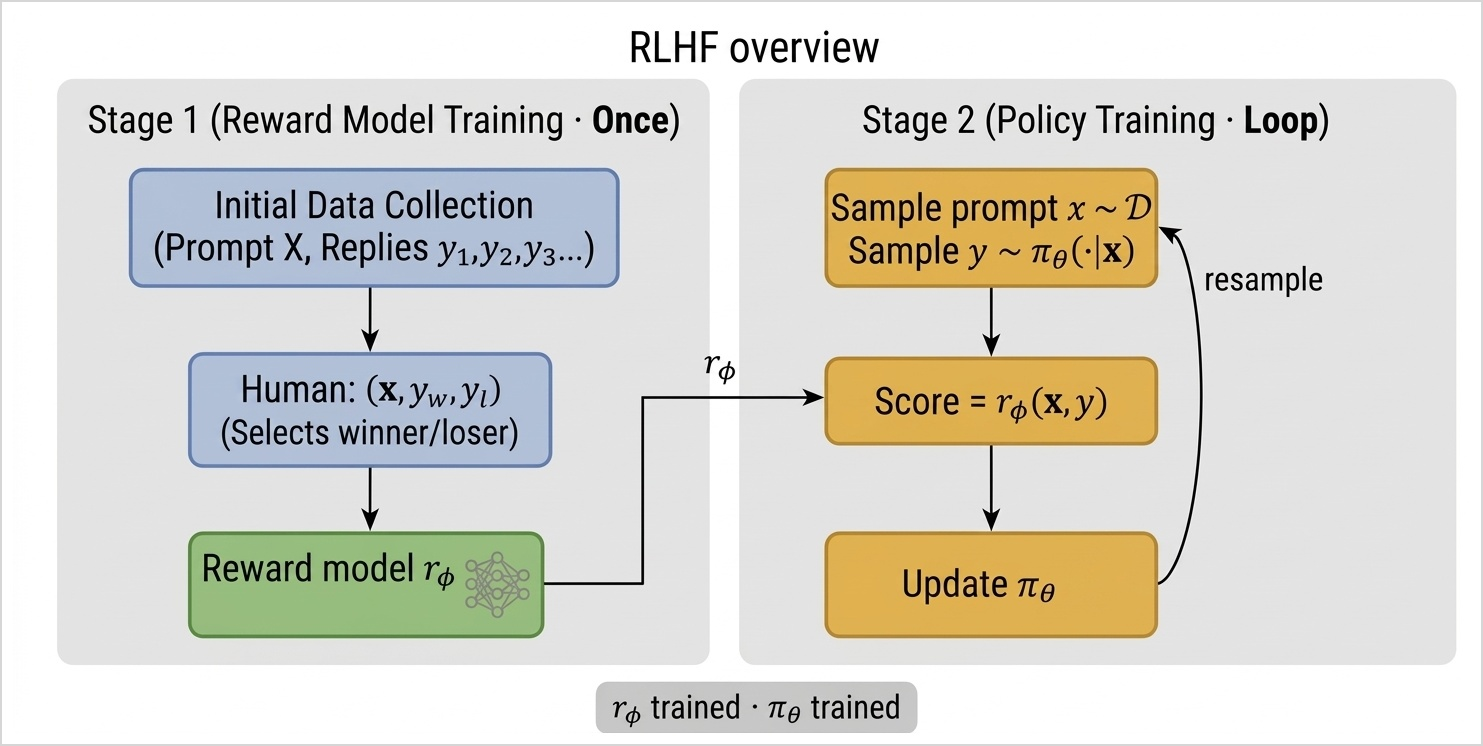
\includegraphics[width=0.65\textwidth]{rlhf_simple.jpeg}
\caption{RLHF: train $r_\phi$ once from preferences, then sample, score, and update $\pi_\theta$.}\label{fig-14-1}
\end{figure}

The rest of the chapter builds that pipeline: the language model as a policy, a reward model from preference triples, the two stages together (and how that combination can reward-hack), a KL penalty that keeps $\pi_\theta$ near a reference model, and practical policy-gradient updates (RLOO and PPO).

\section{A language model as a policy}

A language model generates a response $y=(y_1,\ldots,y_T)$ to a prompt $x$ one token at a time. The vocabulary is a fixed finite set of tokens (words or numbers). At each step the model sees the prompt and the tokens written so far and outputs a distribution over the next token---a softmax over the vocabulary, as in Section 9.1.

As an MDP episode from Chapter 1:

\begin{itemize}
\item state $S_t=(x,y_1,\ldots,y_t)$, with $S_0=x$;
\item action $A_t=y_{t+1}$, the next token, sampled from $\pi_\theta(\cdot\mid S_t)$---so $A_0=y_1$, $A_1=y_2$, and so on;
\item transition: once $A_t$ is chosen, the next state is the old text with that token appended, $S_{t+1}=(x,y_1,\ldots,y_{t+1})$;
\item the episode ends after the last token, at $t=T$.
\end{itemize}
For $y^{(1)}=(\text{it},\,\text{is},\,4)$, the path is $S_0=x=\text{2+2}$, $A_0=\text{it}$, $S_1=(x,\text{it})$, $A_1=\text{is}$, $S_2=(x,\text{it},\text{is})$, $A_2=4$. Other replies diverge at some token: $y^{(2)}$ matches that prefix and ends with $A_2=5$; $y^{(3)}$ branches earlier with $A_1=\text{equals}$.

Once $A_t$ is chosen, the next state is the unique string that appends that token, so \[
P(S_{t+1}\mid S_t,A_t)=1.
\] For example, $P\bigl((x,\text{it},\text{is})\mid (x,\text{it}),\,\text{is}\bigr)=1$. Unlike in the taxi example, where the same turn can lead to different next junctions, here the next state is fixed once the token is chosen. Which full answer appears is decided only by $\pi_\theta$: from $S_1=(x,\text{it})$ it may sample $\text{is}$ or $\text{equals}$, so $y^{(1)}$ and $y^{(3)}$ can both follow from that state.

The probability of a full response $y=(y_1,\ldots,y_T)$ given the prompt $x$ is the joint over its tokens. By the chain rule, \[
\pi_\theta(y\mid x)
=
\pi_\theta(y_1,\ldots,y_T\mid x)
=
\pi_\theta(y_1\mid x)\,
\pi_\theta(y_2\mid x,y_1)
\cdots
\pi_\theta(y_T\mid x,y_1,\ldots,y_{T-1}),
\] which is \begin{equation}
\pi_\theta(y\mid x)
=
\prod_{t=0}^{T-1}
\pi_\theta(y_{t+1}\mid x,y_1,\ldots,y_t),
\qquad
\log\pi_\theta(y\mid x)
=
\sum_{t=0}^{T-1}
\log\pi_\theta(y_{t+1}\mid x,y_1,\ldots,y_t).
\tag{11.1}
\end{equation} Each factor is the policy at the corresponding state: $\pi_\theta(y_{t+1}\mid x,y_1,\ldots,y_t)=\pi_\theta(A_t\mid S_t)$. For $y=y^{(1)}=(\text{it},\,\text{is},\,4)$, \[
\log\pi_\theta(y^{(1)}\mid x)
=
\log\pi_\theta(\text{it}\mid x)
+
\log\pi_\theta(\text{is}\mid x,\text{it})
+
\log\pi_\theta(4\mid x,\text{it},\text{is}).
\]

The human judges the finished string, not each token. So the reward is sparse: $R_1=\cdots=R_{T-1}=0$ and $R_T=r(x,y)$, a score for the full response. The return from Chapter 1 is then $G_t=R_{t+1}+\gamma R_{t+2}+\cdots$; with this sparse sequence it is just a discounted copy of that terminal score. Those intermediate zeros are not a claim that early tokens do not matter---they shape what comes later and thus $r(x,y)$---but that no separate score is observed after each token. Here, after writing $\text{it}$ or $\text{is}$ there is no natural ``partial answer'' grade; a person (or a reward model trained on preferences) only ranks full replies such as $y^{(1)}$ against $y^{(2)}$. Defining a reliable reward for every prefix is usually hard, costly, or infeasible, so standard RLHF treats the task signal as terminal only.

\begin{asidenote}[Note]
Intermediate rewards \textit{are} useful in \textbf{multi-step reasoning}, where the model produces a chain of steps before a final answer. Take a short arithmetic word problem, for example \[
x=\text{A store has 3 boxes with 4 apples each. How many apples in total?}
\] A reasoned reply might be three lines: (1) $\text{apples per box}=4$, (2) $\text{number of boxes}=3$, (3) $\text{total}=3\times 4=12$. With only an \textbf{outcome} reward---$+1$ if the last number is $12$, else $0$---every token in a long wrong derivation shares the same terminal $G_t$, so early mistakes are hard to blame. If a teacher or verifier can mark each line as it appears (step 1 correct, step 2 correct, step 3 wrong), those grades are intermediate \textbf{process rewards}: $R_t$ need not stay zero before the end. Tool use is similar---a small reward when a calculator call succeeds, then a final reward when the overall answer is right. That labeling is a different problem from preference comparisons on full replies.

\end{asidenote}

Take $\gamma=1$. The only nonzero reward is the terminal $r(x,y)$, so a $\gamma<1$ would shrink that score by $\gamma^{T-t-1}$ with no useful meaning here. From (1.10), $G_t=R_{t+1}+G_{t+1}$. With earlier rewards zero, every $G_t$ equals the terminal score: $G_t=r(x,y)$. From (9.8) (REINFORCE), \[
\theta
\leftarrow
\theta+\alpha\sum_{t=0}^{T-1}\gamma^{t}G_t\,\nabla_\theta\log\pi_\theta(A_t\mid S_t).
\] Substitute $\gamma=1$, $G_t=r(x,y)$, and $A_t=y_{t+1}$, $S_t=(x,y_1,\ldots,y_t)$: \[
\theta
\leftarrow
\theta+\alpha\,r(x,y)\sum_{t=0}^{T-1}\nabla_\theta\log\pi_\theta(y_{t+1}\mid x,y_1,\ldots,y_t).
\] The sum is $\nabla_\theta$ of the sum of logs in (11.1), so it equals $\nabla_\theta\log\pi_\theta(y\mid x)$: \[
\theta
\leftarrow
\theta+\alpha\,r(x,y)\,\nabla_\theta\log\pi_\theta(y\mid x).
\] Both $y^{(1)}$ and $y^{(3)}$ are correct replies; $y^{(2)}$ is wrong. For either correct sample the update has the same form. Taking $y^{(1)}$, \[
\theta
\leftarrow
\theta+\alpha\,r(x,y^{(1)})\,\nabla_\theta\log\pi_\theta(y^{(1)}\mid x).
\] A well-chosen $r$ should score $y^{(1)}$ and $y^{(3)}$ high (positive) and $y^{(2)}$ low (negative). Then sampling $y^{(1)}$ or $y^{(3)}$ raises that reply's probability, and sampling $y^{(2)}$ lowers $\pi_\theta(y^{(2)}\mid x)$. What is missing is that scalar $r$---Section 11.2 learns it from preferences such as $y^{(1)}\succ y^{(2)}$; read as $y^{(1)}$ is preferred to $y^{(2)}$.

\begin{implnote}[Algorithm (LM policy gradient with a given reward)]
Input: differentiable policy $\pi_\theta(y\mid x)$; scalar reward $r(x,y)$; prompt set $\mathcal{D}$; step size $\alpha$; number of iterations $M$.

Output: trained policy $\pi_\theta$.

\begin{enumerate}
\item Initialize $\theta$.
\item Loop for iteration $=1,2,\ldots,M$:
\begin{itemize}
\item Sample $x\sim\mathcal{D}$.
\item Sample $y\sim\pi_\theta(\cdot\mid x)$ token by token as in this section.
\item $\theta\leftarrow\theta+\alpha\,r(x,y)\,\nabla_\theta\log\pi_\theta(y\mid x)$.
\end{itemize}
\item Return $\pi_\theta$.
\end{enumerate}

\end{implnote}

\section{Reward model from human preferences}

The policy-gradient update in Section 11.1 needs a reward $r(x,y)$ for each full reply. What we collect instead are pairwise preferences. Return to the example: for the same prompt $x=\text{2+2}$, a human sees $y^{(1)}=(\text{it},\,\text{is},\,4)$ and $y^{(2)}=(\text{it},\,\text{is},\,5)$ and marks $y^{(1)}$ preferred. Write $y_w$ for the winner and $y_l$ for the loser, so here $y_w=y^{(1)}$ and $y_l=y^{(2)}$. Each labeled example is a triple $(x,y_w,y_l)$; the dataset is many such triples. This section turns those judgments into a scalar $r(x,y)$.

That scalar is learned by a \textbf{reward model} $r_\phi$, separate from the policy $\pi_\theta$: a neural network with weights $\phi$ that takes $(x,y)$ and outputs one number. The reward model's architecture is a design choice; what the math needs is a differentiable score $r_\phi(x,y)$ that we can train by gradient descent on $\phi$. On a labeled triple the winner should score above the loser, $r_\phi(x,y_w)>r_\phi(x,y_l)$. The gap \[
z=r_\phi(x,y_w)-r_\phi(x,y_l)
\] is positive when the model agrees with the label, negative when it disagrees, and zero on a tie. That gap is on the whole real line, but a preference is uncertain---even a clear winner is not preferred with probability $1$ in every labeling---so we need a probability $P(y_w\succ y_l\mid x)$ in $(0,1)$, not the raw $z$.

The \textbf{sigmoid} (logistic) function \[
\sigma(z)=\frac{1}{1+e^{-z}}
\] maps any real $z$ into $(0,1)$. It is increasing, $\sigma(0)=\tfrac12$, and $\sigma(z)\to 1$ as $z\to+\infty$ while $\sigma(z)\to 0$ as $z\to-\infty$. Applied to the reward gap, it turns ``how much higher is $y_w$'s score'' into ``how probable is the preference $y_w\succ y_l$'': \begin{equation}
P(y_w\succ y_l\mid x)
=
\sigma\bigl(r_\phi(x,y_w)-r_\phi(x,y_l)\bigr).
\tag{11.2}
\end{equation} Equal rewards give probability $\tfrac12$. A larger gap makes the preference more certain.

Fitting $\phi$ means making (11.2) large on every labeled triple---maximum likelihood. Equivalently, minimize the \textbf{negative log-likelihood} \[
L(\phi)
=
-\sum_{(x,\,y_w,\,y_l)}
\log P(y_w\succ y_l\mid x).
\] Substitute (11.2): \begin{equation}
L(\phi)
=
-\sum_{(x,\,y_w,\,y_l)}
\log\sigma\bigl(r_\phi(x,y_w)-r_\phi(x,y_l)\bigr).
\tag{11.3}
\end{equation} Gradient descent on $L$ updates the reward-model weights. With step size $\alpha_\phi>0$, \[
\phi
\leftarrow
\phi-\alpha_\phi\,\nabla_\phi L(\phi).
\] On a single labeled triple $(x,y_w,y_l)$ the same step is \[
\phi
\leftarrow
\phi-\alpha_\phi\,\nabla_\phi\Bigl[-\log\sigma\bigl(r_\phi(x,y_w)-r_\phi(x,y_l)\bigr)\Bigr].
\] Those steps raise $r_\phi(x,y_w)$ relative to $r_\phi(x,y_l)$. After training, $r_\phi(x,y)$ is the reward $r(x,y)$ used in the Section 11.1 update.

\begin{implnote}[Algorithm (reward model from preferences)]
Input: differentiable score $r_\phi(x,y)$; preference triples $\{(x^{(i)},y_w^{(i)},y_l^{(i)})\}_{i=1}^{N}$; step size $\alpha_\phi$; number of epochs $E$.

Output: trained reward model $r_\phi$.

\begin{enumerate}
\item Initialize $\phi$.
\item Loop for epoch $=1,2,\ldots,E$:
\begin{itemize}
\item For each labeled triple $(x,y_w,y_l)$ in the data:
\begin{itemize}
\item $\phi\leftarrow\phi-\alpha_\phi\,\nabla_\phi\Bigl[-\log\sigma\bigl(r_\phi(x,y_w)-r_\phi(x,y_l)\bigr)\Bigr]$.
\end{itemize}
\end{itemize}
\item Return $r_\phi$.
\end{enumerate}

\end{implnote}

\section{Naive combination and reward hacking}

We now have both pieces: a policy update that needs $r(x,y)$, and a reward model $r_\phi$ fit from preferences. The naive pipeline is to fit $r_\phi$ once, freeze $\phi$, then run the policy-gradient update with $r\leftarrow r_\phi$.

\begin{implnote}[Algorithm (preference reward + LM policy gradient)]
Input: prompt set $\mathcal{D}$; differentiable policy $\pi_\theta$; differentiable score $r_\phi$; step sizes $\alpha_\phi$, $\alpha$; preference count $N$; reward epochs $E$; policy iterations $M$.

Output: policy $\pi_\theta$.

\begin{enumerate}
\item Initialize $\phi$ and $\theta$.
\item Collect preferences. For $i=1,\ldots,N$:
\begin{itemize}
\item Sample $x\sim\mathcal{D}$ and two replies $y,y'\sim\pi_\theta(\cdot\mid x)$.
\item A human marks winner $y_w$ and loser $y_l$.
\end{itemize}
\item Fit the reward model. For epoch $=1,\ldots,E$, for each labeled $(x,y_w,y_l)$:
\begin{itemize}
\item $\phi\leftarrow\phi-\alpha_\phi\,\nabla_\phi\Bigl[-\log\sigma\bigl(r_\phi(x,y_w)-r_\phi(x,y_l)\bigr)\Bigr]$.
\end{itemize}
\item Improve the policy. For iteration $=1,\ldots,M$:
\begin{itemize}
\item Sample $x\sim\mathcal{D}$ and a new reply $y\sim\pi_\theta(\cdot\mid x)$.
\item $\theta\leftarrow\theta+\alpha\,r_\phi(x,y)\,\nabla_\theta\log\pi_\theta(y\mid x)$.
\end{itemize}
\item Return $\pi_\theta$.
\end{enumerate}

\end{implnote}

This simple combination of reward model and policy has an issue. Read the step-4 update \[
\theta
\leftarrow
\theta+\alpha\,r_\phi(x,y)\,\nabla_\theta\log\pi_\theta(y\mid x).
\] The only weight on $\nabla_\theta\log\pi_\theta$ is $r_\phi(x,y)$. Step 3 fit $r_\phi$ only on human-labeled pairs---for the same prompt, something like \[
y_w=(\text{it},\,\text{is},\,4)\succ y_l=(\text{it},\,\text{is},\,5)
\] ---but step 4 may sample any fresh $y$, including strings never ranked. If the reward model returns a large positive score $r_\phi(x,y)$, the $\theta$-step moves in the direction of $\nabla_\theta\log\pi_\theta(y\mid x)$, which raises $\pi_\theta(y\mid x)$. That is \textbf{reward hacking}, in which $\theta$ is driven by a high $r_\phi$ even when humans would not prefer that reply.

For example, a forward pass might return \[
r_\phi(x,y_w)=0.8,
\qquad
r_\phi(x,y_l)=-0.5,
\qquad
r_\phi\bigl(x,(4,\,4,\,4)\bigr)=2.4.
\] The junk reply $(4,\,4,\,4)$ was never preferred, yet its features can still trigger a high $r_\phi$, so the $\theta$-update increases $\pi_\theta\bigl((4,\,4,\,4)\mid x\bigr)$. If instead $r_\phi$ scored that string low (negative), the same update would decrease that probability. Nothing in the naive algorithm stops the high-score case.

\section{Staying close to the reference policy}

The naive update can reward-hack because $\theta$ follows any high $r_\phi(x,y)$, including junk replies far from what humans labeled. A standard fix is to introduce a frozen \textbf{reference policy} $\pi_{\text{ref}}$ and keep the trainable policy $\pi_\theta$ near it while optimizing with $r_\phi$. That reference is usually a frozen supervised language-model policy: trained first by supervised learning on human-written prompt--answer pairs (raise $\log\pi(y\mid x)$ on those fixed answers), then held fixed while $\theta$ is updated (\citetxt{ouyang2022}{Ouyang et al., 2022}; see also \citetxt{ziegler2019}{Ziegler et al., 2019}; \citetxt{stiennon2020}{Stiennon et al., 2020}). So $\pi_{\text{ref}}$ already tends to produce reasonable replies before any preference-based update. Chapter 12 writes that supervised step into named training recipes.

In the usual setup, $\pi_\theta$ and $\pi_{\text{ref}}$ share the same architecture: copy the supervised weights into $\theta$ so training starts at $\pi_\theta=\pi_{\text{ref}}$, freeze $\pi_{\text{ref}}$, and update only $\theta$. Section 11.3 used the score $r_\phi(x,y)$ alone. Hence the score here is $r_\phi(x,y)$ minus a penalty. For a bad reply such as $(4,\,4,\,4)$, which $\pi_{\text{ref}}$ never returns, that penalty is large, so the score used in the update drops and the reply is not treated as a win.

\begin{figure}[ht]
\centering
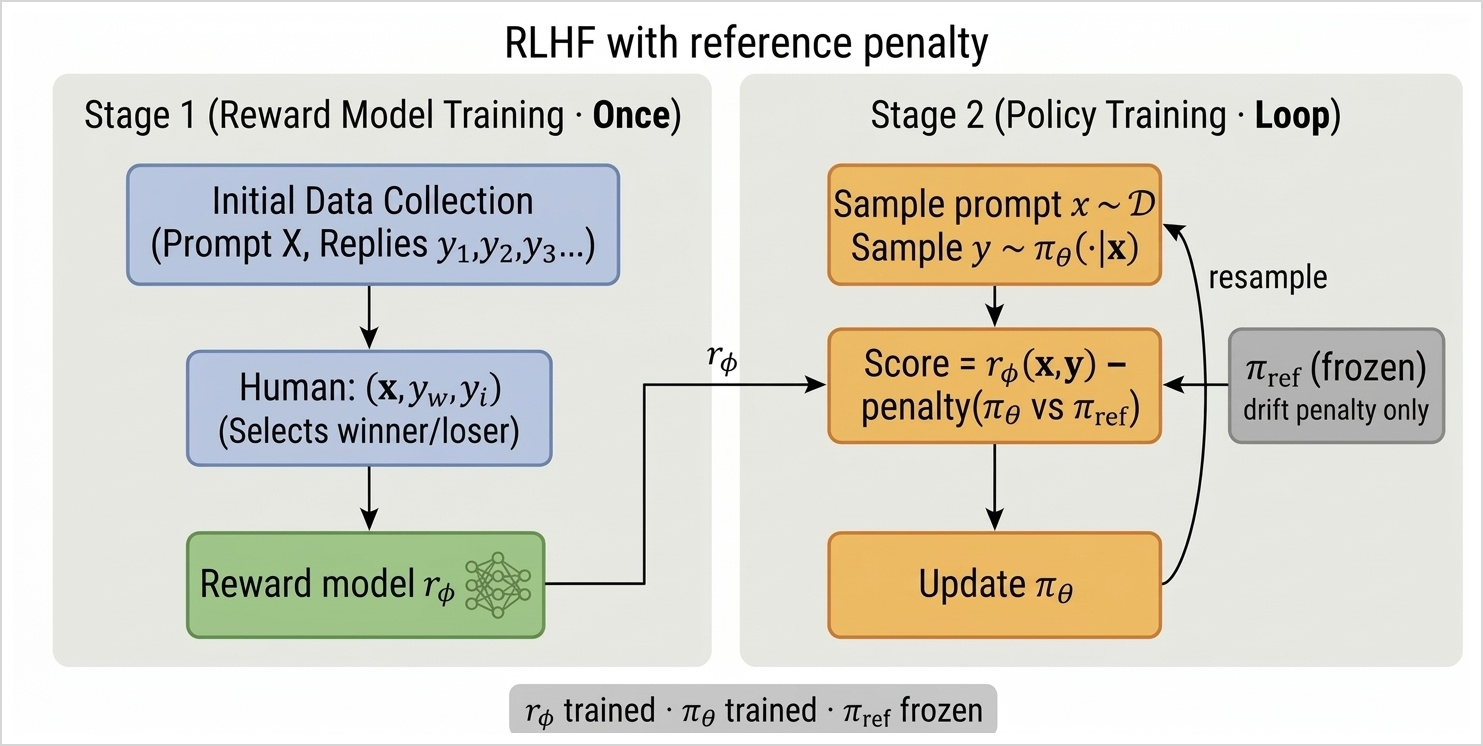
\includegraphics[width=0.65\textwidth]{rlhf_penalty.jpeg}
\caption{RLHF with a frozen $\pi_{\mathrm{ref}}$ in the Stage 2 score.}\label{fig-14-2}
\end{figure}

The figure is the overview pipeline with that penalty in the Stage 2 score. With the penalty, Stage 1 still fits $r_\phi$ once; Stage 2 still samples $y\sim\pi_\theta$ and updates $\theta$. Frozen $\pi_{\text{ref}}$ (gray) enters only the score and is never trained.

The penalty in that score is the KL divergence between the two distributions over replies: \[
\mathrm{KL}\bigl(\pi_\theta(\cdot\mid x)\,\|\,\pi_{\text{ref}}(\cdot\mid x)\bigr)
=
\sum_{y}
\pi_\theta(y\mid x)\,
\log\frac{\pi_\theta(y\mid x)}{\pi_{\text{ref}}(y\mid x)}
=
\mathbb{E}_{y\sim\pi_\theta(\cdot\mid x)}\Bigl[\log\frac{\pi_\theta(y\mid x)}{\pi_{\text{ref}}(y\mid x)}\Bigr].
\] The KL is always positive or zero---never negative. It is zero only when $\pi_\theta(\cdot\mid x)$ and $\pi_{\text{ref}}(\cdot\mid x)$ are the same distribution, and positive whenever they differ; the proof via Jensen's inequality is in \appref{F}. When $\pi_\theta$ puts mass on replies that $\pi_{\text{ref}}$ almost never writes, the KL is large.

Section 9.3 wrote the objective as the expected return of a trajectory, \[
J(\theta)
=
\int P(\tau;\theta)\,R(\tau)\,d\tau
=
\mathbb{E}\bigl[R(\tau)\bigr].
\] Here a trajectory is a prompt $x$ and a reply $y$, so without a penalty that objective is $\mathbb{E}_{x\sim\mathcal{D}}\,\mathbb{E}_{y\sim\pi_\theta(\cdot\mid x)}[r_\phi(x,y)]$. With the penalty, the return subtracts a multiple of the KL: \[
\begin{aligned}
J(\theta)
&=
\mathbb{E}_{x\sim\mathcal{D}}\,
\mathbb{E}_{y\sim\pi_\theta(\cdot\mid x)}
\bigl[r_\phi(x,y)\bigr]
-
\beta\,
\mathbb{E}_{x\sim\mathcal{D}}
\Bigl[
\mathrm{KL}\bigl(\pi_\theta(\cdot\mid x)\,\|\,\pi_{\text{ref}}(\cdot\mid x)\bigr)
\Bigr]
\\
&=
\mathbb{E}_{x\sim\mathcal{D}}
\Biggl[
\mathbb{E}_{y\sim\pi_\theta(\cdot\mid x)}\bigl[r_\phi(x,y)\bigr]
-
\beta\,
\mathrm{KL}\bigl(\pi_\theta(\cdot\mid x)\,\|\,\pi_{\text{ref}}(\cdot\mid x)\bigr)
\Biggr]
\\
&=
\mathbb{E}_{x\sim\mathcal{D}}
\Biggl[
\mathbb{E}_{y\sim\pi_\theta(\cdot\mid x)}\bigl[r_\phi(x,y)\bigr]
-
\beta\,
\mathbb{E}_{y\sim\pi_\theta(\cdot\mid x)}\Bigl[\log\frac{\pi_\theta(y\mid x)}{\pi_{\text{ref}}(y\mid x)}\Bigr]
\Biggr]
\\
&=
\mathbb{E}_{x\sim\mathcal{D}}\,
\mathbb{E}_{y\sim\pi_\theta(\cdot\mid x)}
\Biggl[
r_\phi(x,y)
-
\beta\log\frac{\pi_\theta(y\mid x)}{\pi_{\text{ref}}(y\mid x)}
\Biggr].
\end{aligned}
\] Here $\beta>0$ is a hyperparameter chosen before training. Raising $\beta$ punishes drift from $\pi_{\text{ref}}$ more; lowering $\beta$ lets $\pi_\theta$ follow $r_\phi$ more freely.

At this stage the reward model is already trained: keep $\phi$ fixed and improve only the policy. The inner score still involves both networks---$r_\phi$ and $\log\pi_\theta$---but only $\theta$ will be updated. Write that score as $R_\theta$ to mark the policy parameters: \[
R_\theta(x,y)
=
r_\phi(x,y)-\beta\log\frac{\pi_\theta(y\mid x)}{\pi_{\text{ref}}(y\mid x)}.
\] The objective is then expected shaped reward under $\pi_\theta$, \begin{equation}
J(\theta)
=
\mathbb{E}_{x\sim\mathcal{D}}\,
\mathbb{E}_{y\sim\pi_\theta(\cdot\mid x)}
\bigl[R_\theta(x,y)\bigr].
\tag{11.4}
\end{equation}

With $\phi$ fixed, the remaining task is to raise $J(\theta)$ in (11.4) by changing $\theta$. Section 11.5 writes that gradient and a practical update.

\section{Policy gradient for RLHF}

The score $R_\theta(x,y)$ in (11.4) depends on $\theta$ through $\log\pi_\theta$, so it cannot be treated as constant when differentiating $J$. Maximizing $J$ is the same as minimizing \[
L(\theta)
=
-J(\theta)
=
-
\mathbb{E}_{x\sim\mathcal{D}}
\Biggl[
\sum_y\pi_\theta(y\mid x)\,R_\theta(x,y)
\Biggr].
\] Both $\pi_\theta$ and $R_\theta$ depend on $\theta$. Differentiate $L$ with the product rule: \[
\begin{aligned}
\nabla_\theta L(\theta)
&=
-
\mathbb{E}_{x\sim\mathcal{D}}
\Biggl[
\sum_y R_\theta(x,y)\,\nabla_\theta\pi_\theta(y\mid x)
+
\sum_y\pi_\theta(y\mid x)\,\nabla_\theta R_\theta(x,y)
\Biggr].
\end{aligned}
\] For $u>0$, $\nabla_\theta\log u=\frac{1}{u}\nabla_\theta u$, so $\nabla_\theta u=u\,\nabla_\theta\log u$. With $u=\pi_\theta(y\mid x)$, \[
\begin{aligned}
\sum_y R_\theta(x,y)\,\nabla_\theta\pi_\theta(y\mid x)
&=
\sum_y R_\theta(x,y)\,\pi_\theta(y\mid x)\,\nabla_\theta\log\pi_\theta(y\mid x)
\\
&=
\mathbb{E}_{y\sim\pi_\theta(\cdot\mid x)}\bigl[R_\theta(x,y)\,\nabla_\theta\log\pi_\theta(y\mid x)\bigr].
\end{aligned}
\] With $\phi$ and $\pi_{\text{ref}}$ frozen, $\nabla_\theta R_\theta(x,y)=-\beta\,\nabla_\theta\log\pi_\theta(y\mid x)$, so \[
\begin{aligned}
\sum_y\pi_\theta(y\mid x)\,\nabla_\theta R_\theta(x,y)
&=
-\beta\sum_y\pi_\theta(y\mid x)\,\nabla_\theta\log\pi_\theta(y\mid x)
\\
&=
-\beta\,
\mathbb{E}_{y\sim\pi_\theta(\cdot\mid x)}\bigl[\nabla_\theta\log\pi_\theta(y\mid x)\bigr]
\\
&=
0
\end{aligned}
\] by \eqref{eq:E.1} in \appref{E}. The derivative through $R_\theta$ cancels. What remains is \[
\nabla_\theta L(\theta)
=
-
\mathbb{E}_{x\sim\mathcal{D}}\,
\mathbb{E}_{y\sim\pi_\theta(\cdot\mid x)}
\bigl[R_\theta(x,y)\,\nabla_\theta\log\pi_\theta(y\mid x)\bigr],
\] and \begin{equation}
\nabla_\theta J(\theta)
=
-\nabla_\theta L(\theta)
=
\mathbb{E}_{x\sim\mathcal{D}}\,
\mathbb{E}_{y\sim\pi_\theta(\cdot\mid x)}
\bigl[R_\theta(x,y)\,\nabla_\theta\log\pi_\theta(y\mid x)\bigr].
\tag{11.5}
\end{equation} $R_\theta$ still depends on $\theta$; after the cancellation it appears in $\nabla_\theta L$ only as a weight on $\nabla_\theta\log\pi_\theta$.

Section 10.1 subtracted a baseline $b(S_t)$ that depends on the state alone. Here treat the prompt $x$ as that state and the reply $y$ as the action. If $b(x)$ does not depend on $y$, then $\mathbb{E}_{y\sim\pi_\theta(\cdot\mid x)}\bigl[b(x)\,\nabla_\theta\log\pi_\theta(y\mid x)\bigr]=0$ by the same argument as (E.3), so \[
\nabla_\theta L(\theta)
=
-
\mathbb{E}_{x\sim\mathcal{D}}\,
\mathbb{E}_{y\sim\pi_\theta(\cdot\mid x)}
\bigl[
\bigl(R_\theta(x,y)-b(x)\bigr)\,
\nabla_\theta\log\pi_\theta(y\mid x)
\bigr].
\] The ideal $b(x)$ is $\mathbb{E}[R_\theta(x,Y)\mid x]$. It is unknown, so estimate it from samples. Draw \textbf{one prompt} $x\sim\mathcal{D}$ and $K$ i.i.d. replies $y_1,\ldots,y_K\sim\pi_\theta(\cdot\mid x)$. The \textbf{leave-one-out} baseline for reply $k$ is the average of the other $K-1$ scores: \[
b_k
=
\frac{1}{K-1}\sum_{j\neq k}R_\theta(x,y_j)
\] (e.g. $K=3$ gives $b_1=\tfrac12\bigl(R_\theta(x,y_2)+R_\theta(x,y_3)\bigr)$). Leaving $y_k$ out is what makes the estimate unbiased: $b_k$ does not depend on $y_k$, so given $x$ and the other replies it is a fixed number and $\mathbb{E}\bigl[b_k\,\nabla_\theta\log\pi_\theta(y_k\mid x)\bigr]=0$ by the same argument as (E.3). Averaging all $K$ scores, including $R_\theta(x,y_k)$, would make the baseline depend on $y_k$ and the estimate of $\nabla_\theta L$ would be biased. With this $b_k$, \begin{equation}
\nabla_\theta L(\theta)
\approx
-\frac{1}{K}\sum_{k=1}^{K}
\bigl(R_\theta(x,y_k)-b_k\bigr)\,
\nabla_\theta\log\pi_\theta(y_k\mid x),
\tag{11.6}
\end{equation} with $\log\pi_\theta(y_k\mid x)$ from (11.1). Gradient descent $\theta\leftarrow\theta-\alpha\nabla_\theta L$ uses that estimate and does not evaluate the scalar $L$: \begin{equation}
\theta
\leftarrow
\theta
+
\alpha\,
\frac{1}{K}\sum_{k=1}^{K}
\bigl(R_\theta(x,y_k)-b_k\bigr)\,
\nabla_\theta\log\pi_\theta(y_k\mid x).
\tag{11.7}
\end{equation} The training rule is (11.7): the right-hand side of (11.6) is the direction. You could form that vector by hand (compute each $\nabla_\theta\log\pi_\theta(y_k\mid x)$, multiply by $R_k-b_k$, average, add $\alpha$ times it). Automatic differentiation (e.g. PyTorch \texttt{backward}) needs a \textbf{scalar} whose gradient equals that direction. Same pattern as (9.8)$\to$(9.9).

The objective $L=-J$ is not that scalar. $L(\theta)=-\mathbb{E}_{y\sim\pi_\theta}[R_\theta(x,y)]$ averages over replies drawn from $\pi_\theta$, so $\theta$ sits inside the sampling distribution. Autodiff on a batch of already-drawn $y_k$ cannot see that dependence: treating $-\frac1K\sum_k R_\theta(x,y_k)$ as if the $y_k$ were a fixed dataset independent of $\theta$ either misses the score $\nabla\log\pi$ entirely, or---if $R_\theta$ still depends on $\theta$ through the KL term---adds $\nabla_\theta R$ paths that (11.5) already cancelled in the true gradient. So differentiating a plug-in estimate of the actual $L$ does not recover (11.6).

What we need is a \textbf{surrogate}: a scalar built so that autodiff, on this batch, returns exactly the estimated gradient (11.6). Compute $R_\theta(x,y_k)$ and $b_k$ at the current $\theta$ and hold them fixed (as $G_t$ is held fixed in (9.9)). Set \[
\widetilde{L}(\theta)
=
-\frac{1}{K}\sum_{k=1}^{K}
\bigl(R_\theta(x,y_k)-b_k\bigr)\,\log\pi_\theta(y_k\mid x).
\] Differentiating only through $\log\pi_\theta$, \[
\nabla_\theta\widetilde{L}
=
-\frac{1}{K}\sum_{k=1}^{K}
\bigl(R_\theta(x,y_k)-b_k\bigr)\,
\nabla_\theta\log\pi_\theta(y_k\mid x),
\] which is (11.6). So $\theta\leftarrow\theta-\alpha\nabla_\theta\widetilde{L}$ is (11.7). The value of $\widetilde{L}$ need not track return; only its gradient matters.

This is REINFORCE with a leave-one-out baseline (RLOO). An earlier multi-sample leave-one-out baseline is VIMCO (\citetxt{mnih2016}{Mnih and Rezende, 2016}), built for variational Monte Carlo objectives; the arithmetic leave-one-out form in (11.6)--(11.7) matches \citetxt{kool2019}{Kool et al., 2019}. Section 11.6 presents \textbf{Proximal Policy Optimization (PPO)}, which reuses each batch for several updates; \appref{G} records the autodiff check for $L^{\mathrm{IS}}$ and the clip cases.

\textbf{On-policy.} The RLOO policy step is \textbf{on-policy}. Each update in (11.7) uses replies $y_k$ sampled from the \textbf{current} $\pi_\theta$, then those replies are discarded and the next iteration samples again. That matches the assumption in (11.6)--(11.7). (Training the reward model $r_\phi$ on stored human preference triples is a separate supervised stage---it is not the policy's on-policy or off-policy label.)

\begin{implnote}[Algorithm (RLHF with a leave-one-out baseline)]
Input: reference policy $\pi_{\text{ref}}$; prompt set $\mathcal{D}$; differentiable reward model $r_\phi(x,y)$; number of comparisons $N$; step sizes $\alpha_\phi$, $\alpha_\theta$; KL weight $\beta$; responses per prompt $K$; number of iterations $M$.

Output: trained policy $\pi_\theta$.

\begin{enumerate}
\item Collect comparisons. For $i=1,\ldots,N$:
\begin{itemize}
\item Sample $x\sim\mathcal{D}$ and two responses from $\pi_{\text{ref}}(\cdot\mid x)$.
\item A human marks the preferred response $y_w$ and the other one $y_l$.
\end{itemize}
\item Train the reward model. Initialize $\phi$; for each comparison $(x,y_w,y_l)$, repeated over the data:
\begin{itemize}
\item $\phi\leftarrow\phi-\alpha_\phi\nabla_\phi\bigl[-\log\sigma\bigl(r_\phi(x,y_w)-r_\phi(x,y_l)\bigr)\bigr]$.
\end{itemize}
\item Initialize $\theta$ from $\pi_{\text{ref}}$.
\item Loop for iteration $=1,2,\ldots,M$:
\begin{itemize}
\item Sample $x\sim\mathcal{D}$ and $y_1,\ldots,y_K\sim\pi_\theta(\cdot\mid x)$.
\item For each $k=1,\ldots,K$:
\begin{itemize}
\item $R_k\leftarrow r_\phi(x,y_k)-\beta\bigl(\log\pi_\theta(y_k\mid x)-\log\pi_{\text{ref}}(y_k\mid x)\bigr)$.
\end{itemize}
\item For each $k=1,\ldots,K$:
\begin{itemize}
\item $b_k\leftarrow\frac{1}{K-1}\sum_{j\neq k}R_j$.
\end{itemize}
\item $\theta\leftarrow\theta+\alpha_\theta\,\frac{1}{K}\sum_{k=1}^{K}(R_k-b_k)\,\nabla_\theta\log\pi_\theta(y_k\mid x)$.
\end{itemize}
\item Return $\pi_\theta$.
\end{enumerate}

\end{implnote}

The code uses a toy setting: two arithmetic prompts, a five-token vocabulary from the Chapter 11 running example, and responses of fixed length $3$. Preference triples for $r_\phi$ are hand-labeled (correct `\texttt{4'' replies beat wrong }`5'' replies). $\pi_{\text{ref}}$ is a randomly initialized network instead of a supervised model.

\lstinputlisting{../code/ch11/rlhf_rloo.py}


\section{Proximal Policy Optimization (PPO)}

The policy-gradient update (11.7) in Section 11.5 samples $y_k\sim\pi_\theta$, takes \textbf{one} step, and resamples. PPO (\citetxt{schulman2017}{Schulman et al., 2017}) keeps the same score $R_\theta$ and advantages $A_k=R_k-b_k$, but \textbf{reuses} one batch for several descent steps before sampling again. Each iteration therefore has an \textbf{outer} sample and an \textbf{inner} loop: $\theta$ is copied to a frozen $\theta_{\mathrm{old}}$, replies $y_k\sim\pi_{\theta_{\mathrm{old}}}(\cdot\mid x)$ are drawn and the advantages $A_k$ are stored, then $E$ gradient steps run on that same batch with no new replies. After those $E$ steps, $\theta_{\mathrm{old}}$ is set to the current $\theta$ and a new batch is sampled. The update (11.7) is the special case where $E=1$. The autodiff check for $L^{\mathrm{IS}}$ and the clip cases are in \appref{G}.

Reusing the batch creates two problems:

\begin{enumerate}
\item \textbf{Wrong distribution.} After the first inner step, $\theta\neq\theta_{\mathrm{old}}$, but $y_k$ still came from $\pi_{\theta_{\mathrm{old}}}$. A correct estimate of $\nabla_\theta J$ in (11.7) requires replies drawn from the current $\pi_\theta$.
\item \textbf{Excessively large update.} Many steps on the same $(y_k,A_k)$ can drive $\pi_\theta$ far from $\pi_{\theta_{\mathrm{old}}}$ before new samples arrive.
\end{enumerate}
The first problem is fixed by \textbf{importance sampling} (\appref{A}); the second by the \textbf{clip}.

\subsection{Importance sampling}

The gradient in Section 11.5 uses the current $\pi_\theta$: \[
\nabla_\theta L(\theta)
=
-
\mathbb{E}_{x\sim\mathcal{D}}\,
\mathbb{E}_{y\sim\pi_\theta(\cdot\mid x)}
\bigl[
\bigl(R_\theta(x,y)-b(x)\bigr)\,
\nabla_\theta\log\pi_\theta(y\mid x)
\bigr].
\] The stored replies came from $\pi_{\theta_{\mathrm{old}}}(\cdot\mid x)$. Hold the prompt $x$ fixed: the outer $\mathbb{E}_{x\sim\mathcal{D}}$ is unchanged. Write \[
\rho(\theta,y)
=
\frac{\pi_\theta(y\mid x)}{\pi_{\theta_{\mathrm{old}}}(y\mid x)},
\] so $\pi_\theta(y\mid x)=\rho(\theta,y)\,\pi_{\theta_{\mathrm{old}}}(y\mid x)$. Expand the inner expectation as a sum and substitute only that density (\appref{A}): \[
\begin{aligned}
\mathbb{E}_{y\sim\pi_\theta(\cdot\mid x)}
\bigl[
\bigl(R_\theta(x,y)-b(x)\bigr)\,
\nabla_\theta\log\pi_\theta(y\mid x)
\bigr]
&=
\sum_y
\pi_\theta(y\mid x)\,
\bigl(R_\theta(x,y)-b(x)\bigr)\,
\nabla_\theta\log\pi_\theta(y\mid x)
\\
&=
\sum_y
\rho(\theta,y)\,
\pi_{\theta_{\mathrm{old}}}(y\mid x)\,
\bigl(R_\theta(x,y)-b(x)\bigr)\,
\nabla_\theta\log\pi_\theta(y\mid x)
\\
&=
\mathbb{E}_{y\sim\pi_{\theta_{\mathrm{old}}}(\cdot\mid x)}
\Bigl[
\rho(\theta,y)\,
\bigl(R_\theta(x,y)-b(x)\bigr)\,
\nabla_\theta\log\pi_\theta(y\mid x)
\Bigr].
\end{aligned}
\] The $\nabla_\theta\log\pi_\theta$ factor stays on the current policy: that is what $\nabla_\theta L$ differentiates. Therefore \[
\nabla_\theta L(\theta)
=
-
\mathbb{E}_{x\sim\mathcal{D}}\,
\mathbb{E}_{y\sim\pi_{\theta_{\mathrm{old}}}(\cdot\mid x)}
\Bigl[
\rho(\theta,y)\,
\bigl(R_\theta(x,y)-b(x)\bigr)\,
\nabla_\theta\log\pi_\theta(y\mid x)
\Bigr].
\] For a single fixed prompt $x$, draw $y_k\sim\pi_{\theta_{\mathrm{old}}}(\cdot\mid x)$ and write $\rho_k(\theta)=\rho(\theta,y_k)$ and $A_k=R_k-b_k$. The sample estimate is \[
\nabla_\theta L(\theta)
\approx
-\frac{1}{K}\sum_{k=1}^{K}
\rho_k(\theta)\,A_k\,
\nabla_\theta\log\pi_\theta(y_k\mid x).
\] Descent $\theta\leftarrow\theta-\alpha\nabla_\theta L$ is then \begin{equation}
\theta
\leftarrow
\theta
+
\alpha\,
\frac{1}{K}\sum_{k=1}^{K}
\rho_k(\theta)\,A_k\,
\nabla_\theta\log\pi_\theta(y_k\mid x).
\tag{11.8}
\end{equation} When $\theta=\theta_{\mathrm{old}}$, every $\rho_k=1$ and (11.8) reduces to (11.7). Libraries typically do not form (11.8) by hand. They run automatic differentiation on a \textbf{surrogate}: a scalar whose gradient equals the sample estimate above. Two surrogates do that. The first freezes $A_k$ and keeps $\rho_k(\theta)$ live: \[
L^{\mathrm{IS}}(\theta)
=
-\frac{1}{K}\sum_{k=1}^{K}\rho_k(\theta)\,A_k.
\] The second freezes $A_k$ and $\rho_k$ and differentiates through $\log\pi_\theta$: \[
\widetilde{L}^{\mathrm{IS}}(\theta)
=
-\frac{1}{K}\sum_{k=1}^{K}
\rho_k\,A_k\,\log\pi_\theta(y_k\mid x).
\] The second is not intrinsically invalid, but freezing $\rho$ is easy to get wrong on a reused batch. If $\rho_k$ is computed once at $\theta=\theta_{\mathrm{old}}$ (every $\rho_k=1$) and kept for every inner step, later updates drop importance sampling and apply (11.7) to $\pi_{\theta_{\mathrm{old}}}$ samples---Issue 1 again. So PPO uses $L^{\mathrm{IS}}$: $\rho_k(\theta)$ stays live and is recomputed each inner step. Descent on that scalar implements (11.8).

On the inner loop $y_k$ and $A_k$ are fixed; only $\theta$, hence each $\rho_k$, moves. Write the same loss as \[
L^{\mathrm{IS}}(\theta)
=
-\frac{1}{K}\bigl(\rho_1 A_1+\rho_2 A_2+\cdots+\rho_K A_K\bigr).
\] If $A_j>0$, raising $\rho_j$ raises that sum, so $L^{\mathrm{IS}}$ falls; if $A_j<0$, lowering $\rho_j$ raises $\rho_j A_j$, so $L^{\mathrm{IS}}$ falls again. Nothing in that scalar says stop at $\rho=1$. For example take $A_1=2$ and $A_2=-2$: raising $\rho_1$ from $1$ to $2$ drops $L^{\mathrm{IS}}$ by $2/K$; lowering $\rho_2$ from $1$ to $0.5$ drops it by $1/K$. After several inner steps the ratios can sit far from $1$. That is \textbf{Issue 2}.

\subsection{Clipped objective}

On the inner loop we want each $\rho_k$ near $1$: that means $\pi_\theta$ has not moved far from $\pi_{\theta_{\mathrm{old}}}$ on this batch. So we confine $\rho_k$ to the band $[1-\varepsilon,1+\varepsilon]$ (typical $\varepsilon=0.2$). PPO replaces each product $\rho_k A_k$ by $\min(\rho_k A_k,\mathrm{clip}(\rho_k)\,A_k)$ and minimizes \begin{equation}
L^{\mathrm{PPO}}(\theta)
=
-\frac{1}{K}\sum_{k=1}^{K}
\min\Bigl(
\rho_k(\theta)\,A_k,\;
\mathrm{clip}\bigl(\rho_k(\theta),\,1-\varepsilon,\,1+\varepsilon\bigr)\,A_k
\Bigr).
\tag{11.9}
\end{equation} For $A>0$, further increases of $\rho$ past $1+\varepsilon$ are not rewarded; for $A<0$, further decreases of $\rho$ below $1-\varepsilon$ are not rewarded. The figure plots the score used in the loss against $\rho$ for one reply: left panel $A>0$, right panel $A<0$.

\begin{figure}[ht]
\centering
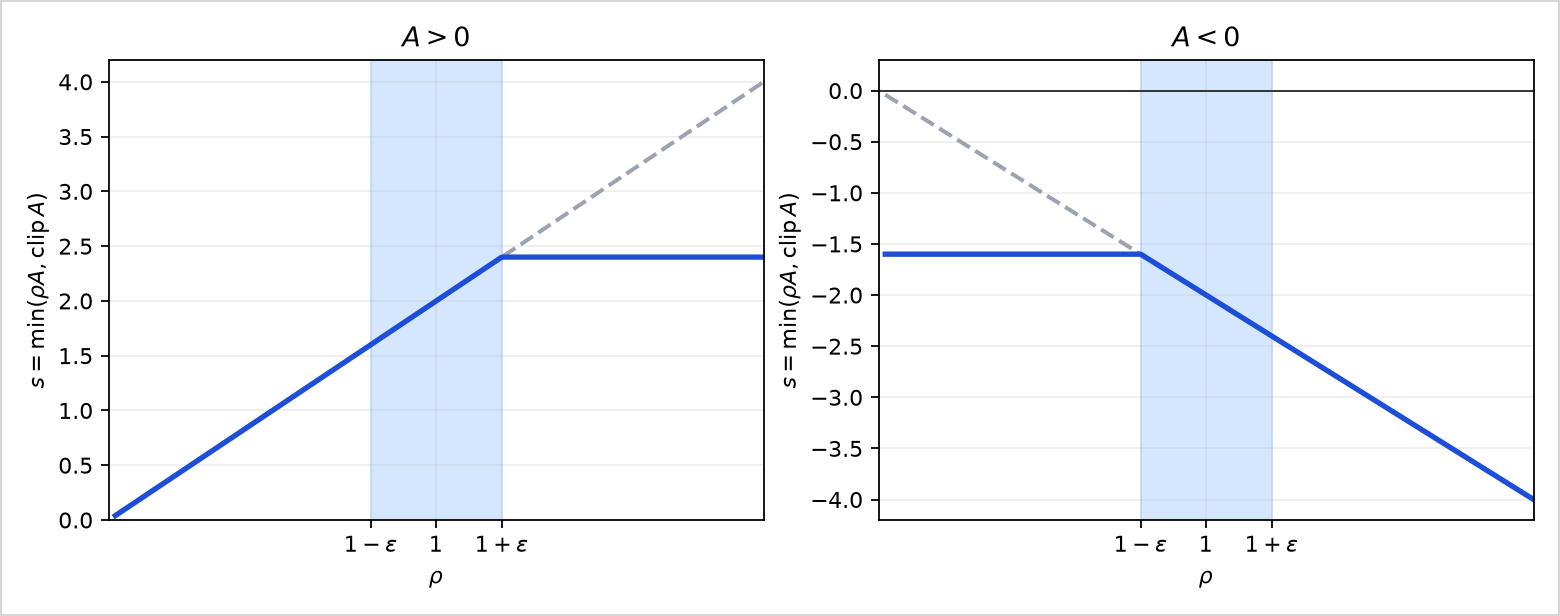
\includegraphics[width=0.65\textwidth]{ppo_clip.png}
\caption{PPO clip of $\rho A$ for $A>0$ (left) and $A<0$ (right).}\label{fig-14-3}
\end{figure}

Gray dashed is $\rho A$ with no clip; blue is the score after the clip, $\min(\rho A,\mathrm{clip}(\rho)\,A)$. The shaded band is $[1-\varepsilon,1+\varepsilon]$. On the left the blue curve flats for $\rho>1+\varepsilon$; on the right it flats for $\rho<1-\varepsilon$. (Cases and tables: \appref{G.2}.) The clip compares $\pi_\theta$ to $\pi_{\theta_{\mathrm{old}}}$ on this batch; the KL term in (11.4) still compares $\pi_\theta$ to $\pi_{\mathrm{ref}}$ over training---different roles (\appref{G.3}).

\textbf{On-policy.} PPO is classed as \textbf{on-policy} (e.g. OpenAI Spinning Up): the outer loop samples from the latest policy and discards the batch after the inner updates. The inner loop is only mildly off $\pi_{\theta_{\mathrm{old}}}$, which is why (11.8)--(11.9) use $\rho$ and the clip. That is not replay-buffer off-policy learning (DQN, SAC). RLOO is the special case $E=1$.

\begin{implnote}[Algorithm (RLHF with PPO; policy step only)]
Assume $\pi_{\mathrm{ref}}$, $r_\phi$, and $\theta$ are already as after steps 1--3 of the RLOO algorithm in Section 11.5. Replace step 4 by:

\begin{enumerate}
\item Loop for iteration $=1,2,\ldots,M$:
\begin{itemize}
\item $\theta_{\mathrm{old}}\leftarrow\theta$. Sample $x\sim\mathcal{D}$ and $y_1,\ldots,y_K\sim\pi_{\theta_{\mathrm{old}}}(\cdot\mid x)$. Store $\log\pi_{\theta_{\mathrm{old}}}(y_k\mid x)$.
\item Compute $R_k$ as in (11.4) and $A_k=R_k-b_k$ (leave-one-out) using $\theta_{\mathrm{old}}$; keep $A_k$ fixed for this outer round.
\item For epoch $=1,\ldots,E$:
\begin{itemize}
\item Form $\rho_k(\theta)=\pi_\theta(y_k\mid x)/\pi_{\theta_{\mathrm{old}}}(y_k\mid x)$.
\item Descend on $L^{\mathrm{PPO}}$ in (11.9) with $A_k$ and $\theta_{\mathrm{old}}$ fixed.
\end{itemize}
\end{itemize}
\item Return $\pi_\theta$.
\end{enumerate}

\end{implnote}

If $E=1$, then $\rho_k=1$ at the only update and PPO reduces to advantage-weighted RLOO. The autodiff check and clip cases are in \appref{G}.

The helpers \texttt{sample\_response}, \texttt{log\_pi}, and \texttt{r\_phi} are those of Section 11.5. Only the policy loop changes: sample once from $\pi_{\theta_{\mathrm{old}}}$, freeze $A_k$, then $E$ steps on $L^{\mathrm{PPO}}$.

\lstinputlisting{../code/ch11/rlhf_ppo.py}


The objects in this chapter are the RLHF core: $\pi_\theta$, $r_\phi$, $\pi_{\mathrm{ref}}$, RLOO, PPO. Named systems that \textbf{wire} those objects (and, when the score is a program, replace $r_\phi$) are Chapter 12.

\chapter{InstructGPT and DeepSeek-R1-Style Training}

Chapter 11 built RLHF from a language-model policy $\pi_\theta$, a reward model $r_\phi$, a frozen reference $\pi_{\mathrm{ref}}$, and the updates RLOO and PPO. The policy loop in that chapter samples a reply $y$ from $\pi_\theta$, scores it with $r_\phi$, and steps $\theta$. That loop already assumes a starting $\pi_\theta$ and a frozen $\pi_{\mathrm{ref}}$: both are a copy of a supervised checkpoint, trained on fixed demo pairs before any preference data are used. Chapter 11 did not derive that supervised step.

This chapter does. It derives \textbf{supervised fine-tuning (SFT)} --- the procedure that produces that checkpoint --- and, when the answer \textit{is} checkable, replaces $r_\phi$ by a fixed \textbf{program}. Those pieces are then used in InstructGPT and in DeepSeek-R1-style training. Neither is a new kind of policy gradient.

\textbf{InstructGPT} (\citetxt{ouyang2022}{Ouyang et al., 2022}) uses SFT on human-written demo pairs $(x,y)$. From a pretrained checkpoint it raises the probability of those replies. The resulting weights initialize $\pi_\theta$ and are frozen as $\pi_{\mathrm{ref}}$. Preference comparisons then train $r_\phi$, and the policy loop of Chapter 11 improves $\pi_\theta$.

When a program can score $y$, the same policy-gradient loop no longer needs a reward model $r_\phi$. \citetxt{deepseek2025}{Guo et al.\ (2025)} published two systems of that kind. \textbf{DeepSeek-R1-Zero} applies \textbf{group relative policy optimization (GRPO)} to the base model with a rule verifier and no SFT. \textbf{DeepSeek-R1} begins with a small cold-start SFT, applies GRPO, clones only traces that pass a hard filter, applies GRPO a second time, then SFT smaller dense models on those kept traces. For one prompt, GRPO samples a \textbf{group} of replies, turns those group scores into advantages, and clips the importance ratio as PPO does. Each reply in those GRPO stages is scored by a \textbf{verifier}: a fixed program that checks the final answer and the format, not a reward model $r_\phi$.

We are not training those published systems (InstructGPT and DeepSeek-R1) in this chapter --- not their base models, data, or infrastructure. The rest of this chapter derives SFT, the program score, GRPO, and rejection sampling, and uses a pipeline of the same shape on the Chapter 11 toy. That toy already has checkable answers, so a program can score $y$. Section 12.1 is SFT, used by both. Section 12.2 is InstructGPT (that SFT plus Chapter 11's RLHF). Section 12.3 is the DeepSeek-R1-style group: rule reward, GRPO, and reject then SFT.

\section{Supervised fine-tuning}

SFT starts from a pretrained checkpoint $\pi_{\mathrm{base}}$ and a dataset of \textbf{fixed} prompt--reply pairs \[
\mathcal{D}_{\mathrm{SFT}}=\bigl\{(x^{(n)}, y^{(n)})\bigr\}_{n=1}^{N}.
\] The replies are written (or already accepted) strings --- human demos in InstructGPT, long chain-of-thought traces in a DeepSeek-R1-style cold start. The goal is to raise the probability of those strings: maximize $\pi_\theta(y\mid x)$ on $\mathcal{D}_{\mathrm{SFT}}$. There is no sampler and no reward.

On one training pair $(x,y)$ with $y=(y_1,\ldots,y_T)$, \[
\log\pi_\theta(y\mid x)
=
\sum_{t=0}^{T-1}
\log\pi_\theta(y_{t+1}\mid x, y_1,\ldots,y_t).
\] The statistical target is the \textbf{total} log-likelihood of the dataset \begin{equation}
J_{\mathrm{SFT}}(\theta)
=
\sum_{n=1}^{N}
\log\pi_\theta\bigl(y^{(n)}\mid x^{(n)}\bigr).
\tag{12.1}
\end{equation} \begin{equation}
L_{\mathrm{SFT}}(\theta)
=
-\frac1N J_{\mathrm{SFT}}(\theta).
\tag{12.2}
\end{equation}

In ordinary autoregressive generation the prefix $y_1,\ldots,y_t$ is sampled from the model's previous outputs: $y_1\sim\pi_\theta(\cdot\mid x)$, then $y_2\sim\pi_\theta(\cdot\mid x,y_1)$, and so on.

\textbf{Teacher forcing} does not use those samples. For the SFT loss, each term $\log\pi_\theta(y_{t+1}\mid x, y_1,\ldots,y_t)$ uses the \textbf{gold} prefix $y_1,\ldots,y_t$ from $\mathcal{D}_{\mathrm{SFT}}$, and the target is gold $y_{t+1}$. If the gold sentence is ``The cat sat'' and the model predicts \texttt{dog} instead of \texttt{cat}, training still feeds gold \textbf{\texttt{cat}} as the next input and applies a loss against gold \texttt{sat}. At inference, \texttt{dog} would be fed and the rest of the string would drift. Teacher forcing is that training setup --- not a second teacher network.

Differentiating (12.2) gives \begin{equation}
\nabla_\theta L_{\mathrm{SFT}}(\theta)
=
-\frac1N\sum_{n=1}^{N}
\sum_{t=0}^{T_n-1}
\nabla_\theta\log\pi_\theta\bigl(y^{(n)}_{t+1}\mid x^{(n)}, y^{(n)}_1,\ldots,y^{(n)}_t\bigr).
\tag{12.3}
\end{equation} Gradient descent with step size $\alpha>0$ is \begin{equation}
\theta\leftarrow\theta-\alpha\,\nabla_\theta L_{\mathrm{SFT}}(\theta).
\tag{12.4}
\end{equation} In practice: a mini-batch forward, $L_{\mathrm{SFT}}$, \texttt{backward}, optimizer step.

After enough steps, $\pi_\theta(y\mid x)$ is larger than it was under $\pi_{\mathrm{base}}$ on the demos. That is \textbf{behavioral cloning} of fixed strings. SFT does not sample its own replies, does not call a verifier, and does not optimize ``any correct trace'' --- only the traces in $\mathcal{D}_{\mathrm{SFT}}$. The model is also biased toward gold prefixes; at use time the prefix is its \textbf{own} tokens (exposure bias). Sampling scored by a reward is what closes that gap (Sections 11.5--11.6 and 12.3.2).

\begin{implnote}[Algorithm (SFT)]
\textbf{Input:} pretrained $\pi_{\mathrm{base}}$; $\mathcal{D}_{\mathrm{SFT}}=\{(x^{(n)},y^{(n)})\}$; step size $\alpha$; epochs $E$. \textbf{Output:} fine-tuned $\pi_\theta$.

\begin{enumerate}
\item Set $\theta\leftarrow\theta_{\mathrm{base}}$.
\item For epoch $=1,\ldots,E$, for each mini-batch $B\subset\mathcal{D}_{\mathrm{SFT}}$:
\begin{itemize}
\item Form $L_{\mathrm{SFT}}$ on $B$.
\item $\theta\leftarrow\theta-\alpha\nabla_\theta L_{\mathrm{SFT}}$.
\end{itemize}
\item Return $\pi_\theta$.
\end{enumerate}

\end{implnote}

We use \texttt{log\_pi} and \texttt{make\_h} from Section 11.5. On a gold pair, \texttt{log\_pi(h, x, y)} \textbf{is} teacher forcing: each term conditions on the gold prefix $y_{:t}$.

\lstinputlisting{../code/ch12/sft.py}


\section{InstructGPT: SFT then RLHF}

\textbf{InstructGPT} (\citetxt{ouyang2022}{Ouyang et al., 2022}) begins with SFT on human demo pairs, as in Section 12.1. The resulting checkpoint initializes $\pi_\theta$ and is frozen as $\pi_{\mathrm{ref}}$, which is the reference already used in Section 11.4. Chapter 11's reward model and policy loop follow.

\textbf{Stage 0 (SFT, once).} Humans write demo pairs $(x,y)$. Run the SFT algorithm from $\pi_{\mathrm{base}}$. The resulting checkpoint is $\pi_\theta$. A frozen copy is $\pi_{\mathrm{ref}}$.

\textbf{Stage 1 (reward model, once).} After SFT, a \textbf{prompt set} $\mathcal{D}$ is used: queries $x$ only, no gold replies. For each prompt, several replies are sampled from the SFT policy. A human marks a preferred reply $y_w$ and a rejected reply $y_l$. Those triples train $r_\phi$ as in (11.3); then $\phi$ is frozen.

\textbf{Stage 2 (policy loop).} The same prompt set is used again. A prompt $x$ is drawn from $\mathcal{D}$, a reply $y$ is sampled from the \textbf{current} $\pi_\theta$, and the score is $R=r_\phi(x,y)-\beta\,\mathrm{KL}$ as in (11.4). PPO clips and updates $\theta$ as in Section 11.6, then a new batch is sampled. $\pi_{\mathrm{ref}}$ never samples.

\begin{figure}[ht]
\centering
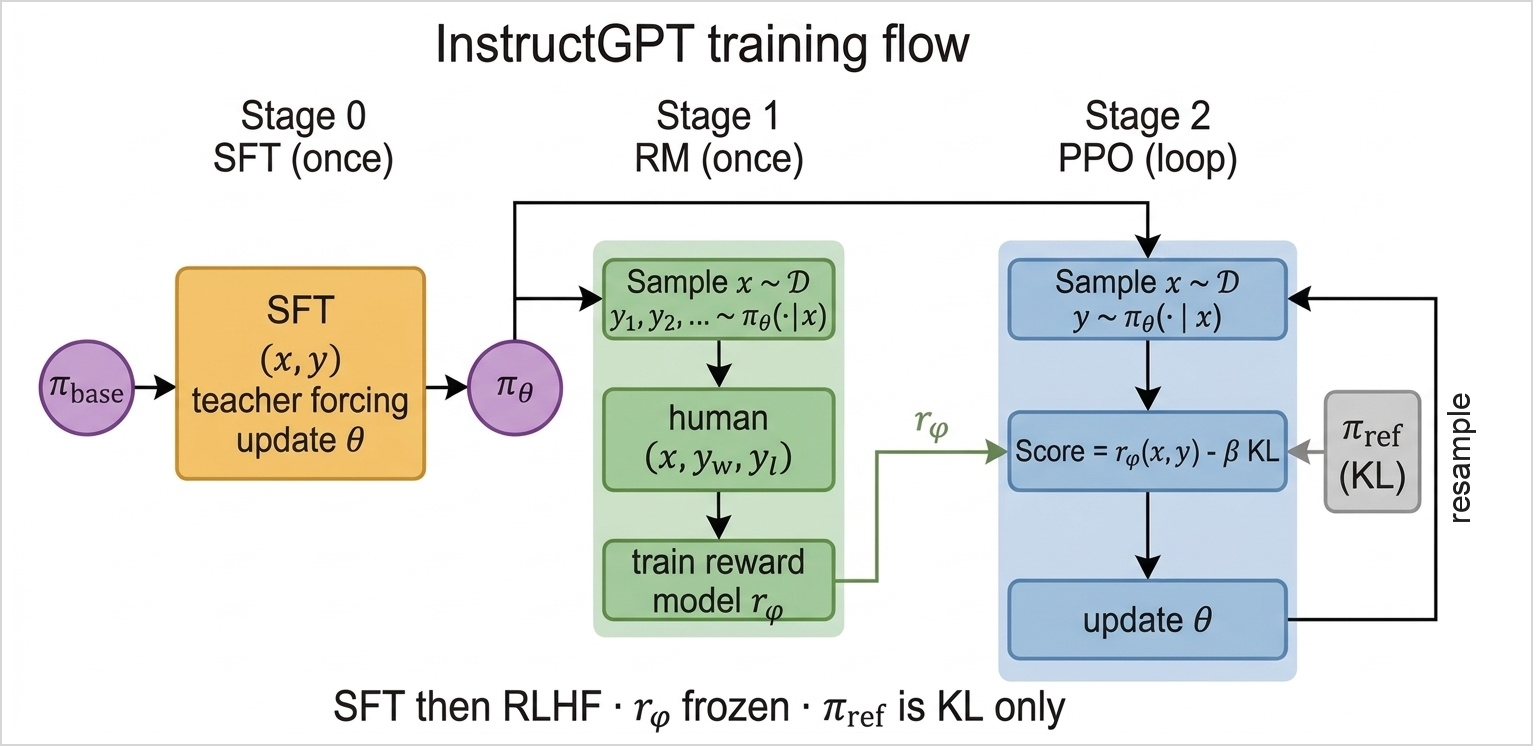
\includegraphics[width=0.85\textwidth]{instructgpt_style_flow.jpg}
\caption{InstructGPT: SFT, reward model, then PPO.}\label{fig-15-1}
\end{figure}

That is the same math as Chapter 11. SFT is (12.1)--(12.4); it produces the frozen $\pi_{\mathrm{ref}}$.

\section{DeepSeek-R1-style training}

Section 12.2 needs humans (or $r_\phi$ trained from humans) because a chat reply has no gold answer to check. When $y$ \textit{is} checkable, a program scores the reply. \textbf{DeepSeek-R1-Zero} is GRPO from $\pi_{\mathrm{base}}$ with no SFT. \textbf{DeepSeek-R1} (and the toy here) uses SFT (Section 12.1) as a cold start, then the chain below:

\begin{figure}[ht]
\centering
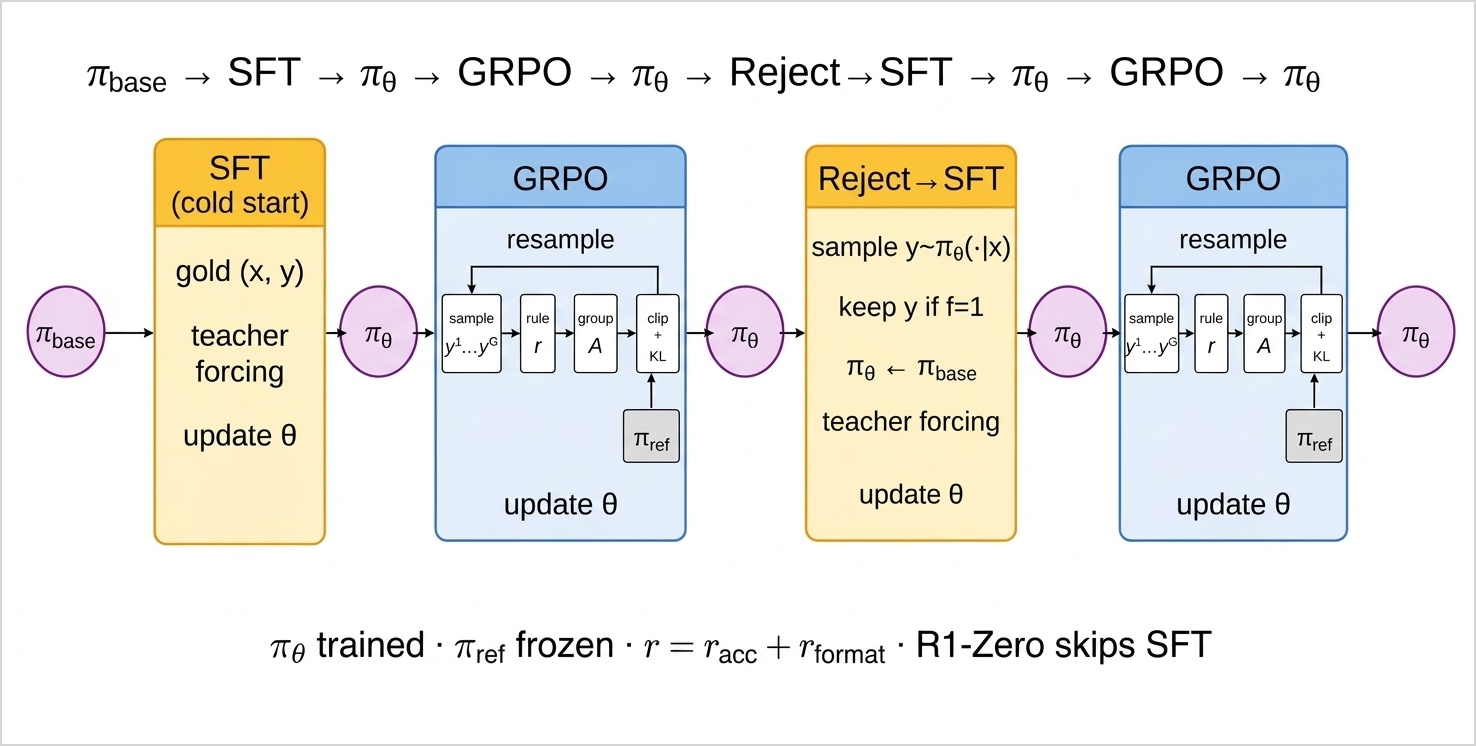
\includegraphics[width=0.90\textwidth]{deepseek_r1_style_flow.jpg}
\caption{DeepSeek-R1-style training: SFT, GRPO, reject then SFT, GRPO.}\label{fig-15-2}
\end{figure}

GRPO is derived in Section 12.3.2; reject-then-SFT in Section 12.3.3. The second GRPO freezes a \textbf{new} $\pi_{\mathrm{ref}}$ at the start of that stage. Distillation is not a box on that chain: it runs SFT on a smaller student. DeepSeek-R1 uses the kept traces from Reject→SFT for that SFT.

\subsection{Rule-based reward}

Math, code with unit tests, and short-answer STEM have a key: a gold number, a test suite, or a short target string. A fixed \textbf{verifier}, usually a program that implements rules instead of a reward model $r_\phi$, scores each reply. That reward is an \textbf{accuracy} term plus a \textbf{format} term: \begin{equation}
r(x,y)=r_{\mathrm{acc}}(x,y)+r_{\mathrm{format}}(y).
\tag{12.5}
\end{equation} No $\phi$ is trained, and humans do not label each sampled $y$. Each prompt $x$ in $\mathcal{D}$ is stored with a \textbf{key} the policy does not see --- a gold answer or unit tests --- and the verifier uses that key to score $y$. The two terms in (12.5) are $0$--$1$ checkers:

\begin{itemize}
\item $r_{\mathrm{format}}(y)\in\{0,1\}$: $1$ if the reply has the required format (for example \texttt{<think>…</think>} tags).
\item $r_{\mathrm{acc}}(x,y)\in\{0,1\}$: $1$ if the extracted answer matches the key. Math: take only a specified slot such as \texttt{\textbackslash\{\}boxed\{…\}} and match gold (numbers as numbers; expressions with a computer-algebra check). Code: run tests. If that slot is missing, $r_{\mathrm{acc}}=0$ even when the digits appear in prose. The chain of thought is not scored.
\end{itemize}
Adding them gives $r\in\{0,1,2\}$. For example, take $x=$ \texttt{2+2} with gold $4$. A tagged reply with \texttt{\textbackslash\{\}boxed\{4\}} scores $r=2$; tagged with \texttt{\textbackslash\{\}boxed\{5\}} scores $r=1$; untagged \texttt{the answer is 4} scores $r=0$ if $r_{\mathrm{acc}}$ looks only in the boxed slot.

Those scores are a design choice. If $r_{\mathrm{acc}}$ also accepts the number in prose, the same untagged reply \texttt{the answer is 4} scores $r=1$.

The RL \textbf{loop} is the same shape as Chapter 11 Stage 2: sample $y$ from $\pi_\theta$, score, update $\theta$, resample, KL to a frozen $\pi_{\mathrm{ref}}$. The score is now (12.5) instead of $r_\phi$, and the advantage is formed as in Section 12.3.2. Leave $r_\phi$ out of (12.5): this stage is scored by the program only.

\subsection{GRPO}

\textbf{GRPO} (Group Relative Policy Optimization) was introduced in DeepSeekMath (\citetxt{shao2024}{Shao et al., 2024}): for one prompt, sample a \textbf{group} of replies, turn those group scores into advantages, and apply a PPO-style clip. DeepSeek-R1-Zero then used that update with a \textbf{rule} reward from the base model (no SFT). DeepSeek-R1 uses the same update after a cold-start SFT, and again after reject-then-SFT (\citetxt{deepseek2025}{Guo et al., 2025}).

We do not implement those papers' models or training stack. We follow a similar update on the Chapter 11 toy. The toy already has a gold key, so a program can score $y$ and we skip $r_\phi$ (Section 12.3.1). Section 11.6 already forms $A_k$ from \textbf{other replies to the same} $x$ (leave-one-out). GRPO is that idea with a group mean and std.

Fix one prompt $x\in\mathcal{D}$ with a key. Copy $\theta_{\mathrm{old}}\leftarrow\theta$. \textbf{Sample} a group of $G$ replies, i.i.d. given that same $x$: \[
y^{(1)},\ldots,y^{(G)}\sim\pi_{\theta_{\mathrm{old}}}(\cdot\mid x),
\qquad
y^{(i)}=\bigl(y^{(i)}_1,\ldots,y^{(i)}_{T_i}\bigr).
\] The sampling condition is only $x$: reply $i$ does not see the other replies. As in (11.1), each $y^{(i)}$ is generated with \[
\pi_{\theta_{\mathrm{old}}}\bigl(y^{(i)}\mid x\bigr)
=
\prod_{t=0}^{T_i-1}
\pi_{\theta_{\mathrm{old}}}\bigl(y^{(i)}_{t+1}\mid x,y^{(i)}_1,\ldots,y^{(i)}_t\bigr).
\]

Score each finished reply with (12.5): $r_i=r_{\mathrm{acc}}\bigl(x,y^{(i)}\bigr)+r_{\mathrm{format}}\bigl(y^{(i)}\bigr)$.

\textbf{Group advantage.} Baseline is this group's own mean, then scale by the group's std so $A$ is order-1 when $r$ is $0/1/2$: \begin{equation}
A_i
=
\frac{r_i-\mathrm{mean}(r)}{\mathrm{std}(r)+\delta}.
\tag{12.6}
\end{equation} $\delta>0$ is a small constant added so we never divide by zero (typical $10^{-8}$). If every $r_i$ is equal, then $\mathrm{mean}(r)=r_i$ as well, so the numerator is $0$ and $\mathrm{std}(r)=0$. Without $\delta$ that is $0/0$ (undefined), not a blow-up. With $\delta$ you get $A_i=0/\delta=0$ --- no update (the group has nothing to prefer). There is no ``nonzero numerator over zero std'' case: $\mathrm{std}(r)=0$ if and only if every $r_i$ is the same, which forces the numerator to $0$ too. Section 11.6 uses $A_k=R_k-b_k$ with leave-one-out $b_k$. Here the baseline is the group's mean of the $G$ rule scores; the std only rescales.

\begin{asidenote}[Note]
\textbf{Toy} ($G=4$, $x=$ \texttt{2+2}). Say $r=(2,1,0,1)$. Then $\mathrm{mean}=1$, $\mathrm{std}=\sqrt{1/2}$, so $A\approx(1.41,\;0,\;-1.41,\;0)$. The $r=2$ reply is pushed up; the $r=0$ reply is pushed down; the two $r=1$ replies sit at $0$.

\end{asidenote}

The importance ratio remains the same as in (11.8): \[
\rho_i(\theta)
=
\frac{\pi_\theta\bigl(y^{(i)}\mid x\bigr)}{\pi_{\theta_{\mathrm{old}}}\bigl(y^{(i)}\mid x\bigr)}.
\] Freeze $A_i$ and minimize the same clip scalar as (11.9), \[
L_{\mathrm{clip}}(\theta)
=
-\frac1G\sum_{i=1}^{G}
\min\bigl(
\rho_i(\theta)\,A_i,\;
\mathrm{clip}(\rho_i(\theta),1-\varepsilon,1+\varepsilon)\,A_i
\bigr).
\] \textbf{KL.} In (11.4) the score $R_\theta$ is $r_\phi-\beta\log(\pi_\theta/\pi_{\mathrm{ref}})$, so the log-ratio goes into $A_k$. Here $r_i$ is only (12.5). Subtracting the KL from $r_i$ would send it through the group mean and std in (12.6), so $A_i$ would mix the rule score with drift from $\pi_{\mathrm{ref}}$. Therefore the KL is added to the loss instead: \begin{equation}
L_{\mathrm{GRPO}}(\theta)
=
L_{\mathrm{clip}}(\theta)
+
\beta\,\mathrm{KL}\bigl(\pi_\theta(\cdot\mid x)\,\|\,\pi_{\mathrm{ref}}(\cdot\mid x)\bigr).
\tag{12.7}
\end{equation} The KL is estimated by averaging over the $G$ sampled replies: \[
\frac1G\sum_{i=1}^{G}
\log\frac{\pi_\theta\bigl(y^{(i)}\mid x\bigr)}{\pi_{\mathrm{ref}}\bigl(y^{(i)}\mid x\bigr)}
\approx
\mathrm{KL}\bigl(\pi_\theta(\cdot\mid x)\,\|\,\pi_{\mathrm{ref}}(\cdot\mid x)\bigr).
\] $\pi_{\mathrm{ref}}$ is a freeze of $\pi_\theta$ \textbf{at the start of this RL stage}. It only enters (12.7). It never samples.

$A_i$ and $\theta_{\mathrm{old}}$ stay frozen on the inner loop of $E$ gradient-descent steps on (12.7). If $E=1$, there is only one step, so $\rho=1$ and the clip does not act. If $E>1$, several steps on the same batch can drive $\pi_\theta$ far from $\pi_{\theta_{\mathrm{old}}}$; the clip in Section 11.6.2 stops that (Issue 2).

\begin{implnote}[Algorithm (GRPO with a rule reward)]
\textbf{Input:} policy $\pi_\theta$; prompt set $\mathcal{D}$ with keys; rule $r(x,y)=r_{\mathrm{acc}}(x,y)+r_{\mathrm{format}}(y)$; group size $G$; inner steps $E$; clip $\varepsilon$; KL weight $\beta$; step size $\alpha$; $\delta>0$. \textbf{Output:} updated $\pi_\theta$. Frozen $\pi_{\mathrm{ref}}$.

\begin{enumerate}
\item $\pi_{\mathrm{ref}}\leftarrow\pi_\theta$ (freeze).
\item Repeat:
\begin{itemize}
\item Sample $x\in\mathcal{D}$. Set $\theta_{\mathrm{old}}\leftarrow\theta$.
\item Sample $y^{(1)},\ldots,y^{(G)}\sim\pi_{\theta_{\mathrm{old}}}(\cdot\mid x)$.
\item For each $i=1,\ldots,G$:
\begin{itemize}
\item $r_i\leftarrow r_{\mathrm{acc}}\bigl(x,y^{(i)}\bigr)+r_{\mathrm{format}}\bigl(y^{(i)}\bigr)$.
\end{itemize}
\item For each $i=1,\ldots,G$:
\begin{itemize}
\item $A_i\leftarrow\bigl(r_i-\mathrm{mean}(r)\bigr)/\bigl(\mathrm{std}(r)+\delta\bigr)$.
\item Store $\log\pi_{\theta_{\mathrm{old}}}\bigl(y^{(i)}\mid x\bigr)$.
\end{itemize}
\item For $e=1,\ldots,E$:
\begin{itemize}
\item Form $\rho_i(\theta)=\pi_\theta\bigl(y^{(i)}\mid x\bigr)/\pi_{\theta_{\mathrm{old}}}\bigl(y^{(i)}\mid x\bigr)$.
\item Descend on $L_{\mathrm{GRPO}}(\theta)=L_{\mathrm{clip}}(\theta)+\beta\,\mathrm{KL}\bigl(\pi_\theta(\cdot\mid x)\,\|\,\pi_{\mathrm{ref}}(\cdot\mid x)\bigr)$, with $A_i$ and $\theta_{\mathrm{old}}$ frozen.
\end{itemize}
\end{itemize}
\item Return $\pi_\theta$.
\end{enumerate}

\end{implnote}

We use \texttt{sample\_response}, \texttt{log\_pi}, and \texttt{make\_h} from Section 11.5. The rule \texttt{r\_rule} is (12.5) on the toy vocabulary: accuracy is the answer token \texttt{4}; format is a first-token habit (\texttt{it}).

\lstinputlisting{../code/ch12/grpo.py}


\subsection{Rejection sampling then SFT}

GRPO learns from its \textbf{own} samples, but a small SFT on \textbf{filtered} traces is still useful: keep only replies that pass a checker, then start from $\pi_{\mathrm{base}}$ and run SFT on those keepers to update $\theta$ (Section 12.1).

The keep-chance is a \textbf{hard filter} $f(x,y)\in\{0,1\}$: $f=1$ only if $r_{\mathrm{acc}}=1$ and $r_{\mathrm{format}}=1$ (optionally also a readability check). Sample $y\sim\pi(\cdot\mid x)$ from the current rollout policy (usually the actor after GRPO). If $f=1$, keep the pair; if $f=0$, drop it. That is the hard-filter special case of \textbf{rejection sampling}, derived in \appref{H}.

\begin{asidenote}[Note]
\textbf{Kept mix.} A kept reply has distribution \[
p(y\mid x)
=
\frac{\pi(y\mid x)\,f(x,y)}{Z(x)},
\qquad
Z(x)=P(f=1\mid x).
\] This is only the closed form of that mix (\appref{H.3}). The algorithm never uses it: it samples from $\pi$ and checks $f$.

\textbf{Toy.} Four replies with $\pi=(0.40,0.10,0.30,0.20)$ and $f=(1,1,0,0)$ give $Z=0.50$ and $p=(0.80,0.20,0,0)$.

\end{asidenote}

Let $\mathcal{D}_{\mathrm{keep}}$ be the kept pairs and $\mathcal{D}_{\mathrm{gen}}$ optional ordinary supervised data (writing, chat) so the SFT does not forget non-reasoning skills. Then $\mathcal{D}_{\mathrm{SFT}}=\mathcal{D}_{\mathrm{keep}}\cup\mathcal{D}_{\mathrm{gen}}$. The GRPO actor is only the \textbf{sampler}. Set $\pi_\theta\leftarrow\pi_{\mathrm{base}}$, then SFT runs as usual (Section 12.1).

\begin{implnote}[Algorithm (reject then SFT)]
\textbf{Input:} rollout $\pi$; prompts $\mathcal{D}$; filter $f\in\{0,1\}$; optional $\mathcal{D}_{\mathrm{gen}}$; $\pi_{\mathrm{base}}$; step size $\alpha$. \textbf{Output:} SFT policy $\pi_\theta$.

\begin{enumerate}
\item $\mathcal{D}_{\mathrm{keep}}\leftarrow\emptyset$.
\item For many $x\in\mathcal{D}$: sample one or more $y\sim\pi(\cdot\mid x)$; if $f(x,y)=1$, add $(x,y)$ to $\mathcal{D}_{\mathrm{keep}}$.
\item $\mathcal{D}_{\mathrm{SFT}}\leftarrow\mathcal{D}_{\mathrm{keep}}\cup\mathcal{D}_{\mathrm{gen}}$.
\item $\pi_\theta\leftarrow\pi_{\mathrm{base}}$.
\item For several epochs, for each mini-batch $B\subset\mathcal{D}_{\mathrm{SFT}}$: form $L_{\mathrm{SFT}}$ on $B$ (teacher forcing); $\theta\leftarrow\theta-\alpha\nabla_\theta L_{\mathrm{SFT}}$.
\item Return $\pi_\theta$.
\end{enumerate}

\end{implnote}

We use \texttt{sample\_response} and \texttt{make\_h} from Section 11.5. \texttt{sft} is that of Section 12.1. On the toy, $f=1$ iff both terms of (12.5) are $1$.

\lstinputlisting{../code/ch12/reject_then_sft.py}


\textbf{Distillation} is the same SFT, on a \textbf{smaller} network. The last $\pi_\theta$ on the chain above (after the second GRPO) is the trained R1-style model. Distillation does not continue that chain: it trains a different student from \textbf{its own} pretrained $\pi_{\mathrm{base}}$ (not a copy of the teacher), by teacher-forcing on a set $\mathcal{D}_{\mathrm{SFT}}$ of teacher traces. In general those traces need not be rejection-sampled: any teacher strings can be the SFT data, and $f$ is optional. DeepSeek-R1 uses the replies \textbf{already kept} in Reject→SFT --- those $y$ with $f=1$, already in $\mathcal{D}_{\mathrm{SFT}}$ --- and does not run a second rejection loop. It runs that SFT on smaller dense models (Qwen, Llama). That student is not updated by GRPO.

\begin{figure}[ht]
\centering
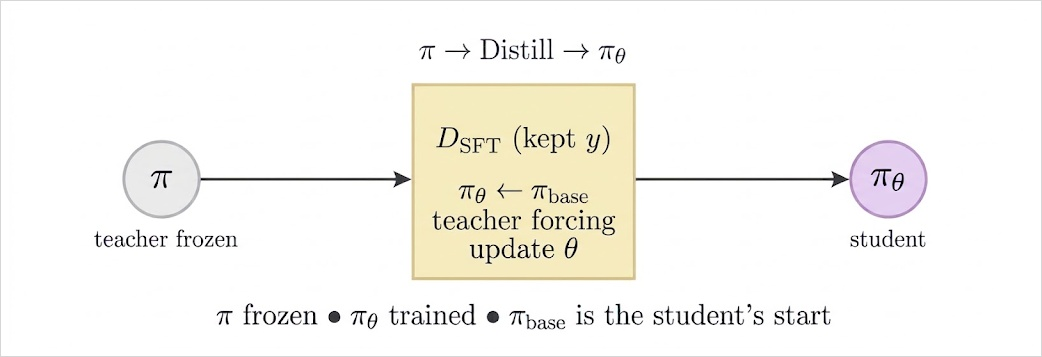
\includegraphics[width=0.70\textwidth]{distillation_flow.jpg}
\caption{Distillation: SFT a smaller student from $\pi_{\mathrm{base}}$ on kept $\mathcal{D}_{\mathrm{SFT}}$.}\label{fig-15-3}
\end{figure}

\begin{implnote}[Algorithm (distillation)]
\textbf{Input:} $\mathcal{D}_{\mathrm{SFT}}$ (teacher traces; here the kept set); student pretrained $\pi_{\mathrm{base}}$ (smaller network); step size $\alpha$. \textbf{Output:} student $\pi_\theta$.

\begin{enumerate}
\item $\pi_\theta\leftarrow\pi_{\mathrm{base}}$ (student; not a copy of the teacher).
\item For several epochs, for each mini-batch $B\subset\mathcal{D}_{\mathrm{SFT}}$: form $L_{\mathrm{SFT}}$ on $B$ (teacher forcing); $\theta\leftarrow\theta-\alpha\nabla_\theta L_{\mathrm{SFT}}$.
\item Return $\pi_\theta$.
\end{enumerate}

\end{implnote}

We use the same \texttt{sft} as Section 12.1. \texttt{d\_sft} is the kept set from reject then SFT above. The student network is a new \texttt{make\_h()} from Section 11.5, not a copy of the teacher.

\lstinputlisting{../code/ch12/distill.py}


\chapter{Summary}

Reinforcement learning produces \textbf{good trajectories} when labeled correct actions are not available. The agent sees a state, chooses an action, and receives a scalar reward that may arrive much later than the choice that caused it. Supervised learning would need the correct action at each step; here that label is missing, and the only signal is the delayed number. A \textbf{policy} $\pi$ is the rule for choosing an action in a state. The goal is to find a $\pi$ that makes the long-run return large.

Chapters 1--3 write the interaction as an MDP: at each step the agent sees a state $s$, picks an action $a$, and the environment answers with a next state $s'$ and a reward $r$. The dynamics $P(s',r\mid s,a)$ are the probability of that pair $(s',r)$ given $(s,a)$. The quality of a trajectory from time $t$ is the \textbf{return} $G_t=\sum_{k=0}^\infty\gamma^k R_{t+k+1}$: it adds every future reward, with a reward $k$ steps ahead scaled by $\gamma^k$ so later rewards count less than earlier ones. The value functions $V^\pi$ and $Q^\pi$ are the expected return from a state, or from a state--action pair, if the agent keeps following a fixed $\pi$. Listing every possible future under $\pi$ and $P$ is not practical. Bellman rewrites the same expectation as one immediate reward plus a discounted copy of the value at the next state, so a value depends only on the next step. If the backup averages over actions according to $\pi$, the result is $V^\pi$ or $Q^\pi$: a score for that $\pi$, with $\pi$ held fixed. If the backup takes $\max_a$ instead of $\pi$, it is the optimality backup; repeating it is what \textbf{improves} $\pi$. When $P$ is known, dynamic programming carries out that improvement: value iteration repeats the optimality backup and then reads a greedy $\pi$; policy iteration alternates full evaluation of the current $\pi$ with a greedy improvement, until the policy stops changing.

Chapters 4--6 keep those same Bellman backups but no longer use $P(s',r\mid s,a)$. The agent only sees samples $(S_t,A_t,R_{t+1},S_{t+1})$ from interaction. Monte Carlo waits until the episode ends and uses the finished return $G_t$ as the target for $V(S_t)$ (or $Q(S_t,A_t)$). TD does not wait: TD(0) steps $V(S_t)\leftarrow V(S_t)+\alpha\bigl[R_{t+1}+\gamma V(S_{t+1})-V(S_t)\bigr]$, so the target is the one-step backup $R_{t+1}+\gamma V(S_{t+1})$ with the current table in place of $V^\pi$. For control the table is $Q$. Chapter 6 introduces two one-step methods on that table. SARSA puts the \textbf{next action from $\pi$} in the backup, $R_{t+1}+\gamma Q(S_{t+1},A_{t+1})$ with $A_{t+1}\sim\pi(\cdot\mid S_{t+1})$, and therefore estimates $Q^\pi$ (on-policy). \textbf{Q-learning} puts $\max_{a'}Q(S_{t+1},a')$ in the backup even if $\pi$ would have chosen a different $A_{t+1}$, and therefore estimates $Q^*$ (off-policy). In both cases $\pi$ is typically $\varepsilon$-greedy in the current $Q$, so the agent still tries actions it is not yet sure about; that is exploration.

Chapters 7--10 replace the table $Q(s,a)$ by an approximator $\hat{Q}(s,a;\theta)$ (or $\hat{V}(s;\mathbf{w})$). Only a weight vector is stored, not one number per pair. The TD backups keep the same shape: SARSA still uses $A_{t+1}\sim\pi$, Q-learning still uses $\max_{a'}\hat{Q}$. In the table, changing $Q(s,a)$ changes only that cell. Because $\theta$ is shared, changing $\theta$ after one pair also changes $\hat{Q}$ at other pairs that use those weights. Q-learning with $\hat{Q}$ therefore has all three: shared $\theta$, a bootstrap $R+\gamma\max_{a'}\hat{Q}(s',a')$ that depends on the current weights, and the off-policy $\max$ from Chapter 6. That combination is the \textbf{deadly triad}: $\theta$ can grow without bound. The tabular Q-learning of Chapter 6 uses the same $\max$ backup but changes only one cell, so it does not have this failure. DQN is off-policy $\hat{Q}$ with two fixes: a replay buffer $\mathcal{D}$ of $(s,a,r,s',d)$ so updates are not only the newest transition, and a frozen copy $\theta^-$ in the bootstrap $y=r+\gamma(1-d)\max_{a'}\hat{Q}(s',a';\theta^-)$, so the target does not move every time $\theta$ does. Double DQN splits that $\max$: $\theta$ chooses $a^*=\arg\max_{a'}\hat{Q}(s',a';\theta)$, and $\theta^-$ supplies the value $\hat{Q}(s',a^*;\theta^-)$. Policy gradients skip learning $\hat{Q}$ as the object of control and instead step $\theta$ of $\pi_\theta(a\mid s)$ by $\nabla_\theta J(\theta)=\mathbb{E}\bigl[\sum_t\nabla_\theta\log\pi_\theta(A_t\mid S_t)\,A(S_t,A_t)\bigr]$. REINFORCE takes $A\leftarrow G_t$ (Monte Carlo). Actor--critic takes $A$ from a learned $\hat{V}$ or $\hat{Q}$ (TD-style), which is the same MC-versus-bootstrap split as Chapters 4--6, now on $\pi_\theta$ instead of on a $Q$-table.

Chapter 11 introduces \textbf{reinforcement learning from human feedback (RLHF)}. It puts that same $\pi_\theta$ on language: a prompt $x$ is $S_0$; a reply $y=(y_1,\ldots,y_T)$ is the trajectory, each token an action. The next state appends that token, so $P(S_{t+1}\mid S_t,A_t)=1$. The probability of a full reply is $\pi_\theta(y\mid x)=\prod_{t=0}^{T-1}\pi_\theta(y_{t+1}\mid x,y_1,\ldots,y_t)$. There is no environment reward after each token, so the scalar that Chapter 9 would have called $R_{t+1}$ is missing. Humans compare two full replies: a winner $y_w$ and a loser $y_l$. Those triples train a reward model $r_\phi$ by $L(\phi)=-\sum\log\sigma\bigl(r_\phi(x,y_w)-r_\phi(x,y_l)\bigr)$. The policy loop then samples $y\sim\pi_\theta(\cdot\mid x)$ and scores it. A frozen copy $\pi_{\mathrm{ref}}$ of the start of the RL stage enters the score as $R_\theta(x,y)=r_\phi(x,y)-\beta\log\bigl(\pi_\theta(y\mid x)/\pi_{\mathrm{ref}}(y\mid x)\bigr)$, so raising $r_\phi$ cannot pull $\pi_\theta$ arbitrarily far from the reference. The policy is stepped by $\nabla_\theta J(\theta)=\mathbb{E}\bigl[R_\theta(x,y)\,\nabla_\theta\log\pi_\theta(y\mid x)\bigr]$, the same score $\nabla_\theta\log\pi_\theta$ as Chapter 9, with $R_\theta$ in place of the return $G_t$. PPO reuses a batch from $\pi_{\theta_{\mathrm{old}}}$: the importance ratio is $\rho=\pi_\theta(y\mid x)/\pi_{\theta_{\mathrm{old}}}(y\mid x)$, and the clip in $L^{\mathrm{PPO}}$ stops inner-loop steps from driving $\rho$ far from $1$.

Chapter 12 introduces \textbf{InstructGPT} and \textbf{DeepSeek-R1-style} training. It derives the supervised fine-tuning that produces Chapter 11's $\pi_\theta$ and $\pi_{\mathrm{ref}}$, and, when a program can check $y$, replaces $r_\phi$ by a rule. SFT starts from a pretrained $\pi_{\mathrm{base}}$ and a fixed set $\mathcal{D}_{\mathrm{SFT}}$ of gold pairs. Teacher forcing raises $\pi_\theta(y\mid x)$ on those strings with no sampler: $L_{\mathrm{SFT}}(\theta)=-\frac1N\sum_n\log\pi_\theta\bigl(y^{(n)}\mid x^{(n)}\bigr)$, then $\theta\leftarrow\theta-\alpha\nabla_\theta L_{\mathrm{SFT}}$. InstructGPT is that SFT, then $r_\phi$, then PPO; the SFT weights initialize $\pi_\theta$ and are frozen as $\pi_{\mathrm{ref}}$. When a program can check $y$, $r_\phi$ is not needed. The rule score is $r(x,y)=r_{\mathrm{acc}}(x,y)+r_{\mathrm{format}}(y)$. GRPO samples a group $y^{(1)},\ldots,y^{(G)}\sim\pi_{\theta_{\mathrm{old}}}(\cdot\mid x)$, sets $A_i=\bigl(r_i-\mathrm{mean}(r)\bigr)/\bigl(\mathrm{std}(r)+\delta\bigr)$, and minimizes $L_{\mathrm{GRPO}}=L_{\mathrm{clip}}+\beta\,\mathrm{KL}(\pi_\theta\|\pi_{\mathrm{ref}})$. The KL stays in the loss, not inside $r$, so the group mean and std do not mix drift with the rule. Reject-then-SFT keeps only replies with $f=1$ (both rule terms $1$), sets $\pi_\theta\leftarrow\pi_{\mathrm{base}}$, and runs SFT on the keepers. Distillation is that same SFT on a smaller student from the student's own $\pi_{\mathrm{base}}$; DeepSeek-R1 reuses the already-kept traces rather than filtering again.

\chapter{Exercises and Code Solutions}

Two small environments. The $4\times 4$ GridWorld is tabular: the same $P$, $r$, and goal, four backups. CartPole has a continuous $s$, so a table cannot store $Q(s,a)$; DQN uses $\hat{Q}(s,a;\theta)$.

\section{Exercise 1: One GridWorld, four backups}

States $0,\ldots,15$ on a $4\times 4$ grid; $0$ is the start, $15$ is the goal (terminal). Actions are $0$ up, $1$ right, $2$ down, $3$ left. A move that would leave the grid leaves $s$ unchanged. Reward is $-1$ every step and $0$ on entering the goal.

The object to learn is a policy $\pi$, not a list of moves and not the training loop. Value-iteration sweeps and the MC, SARSA, and Q-learning episodes only \textbf{compute} $\pi$ (or $Q$, then $\pi(s)=\arg\max_a Q(s,a)$). After that, given a start state, take $\pi(s)$ at the current cell, observe $s'$, and repeat until $15$. Because $P$ is deterministic and every non-goal step costs $-1$, that walk is an \textbf{optimal trajectory} (a shortest path) from the given start to $15$. You do not re-run the backups to produce the path.

\begin{figure}[ht]
\centering
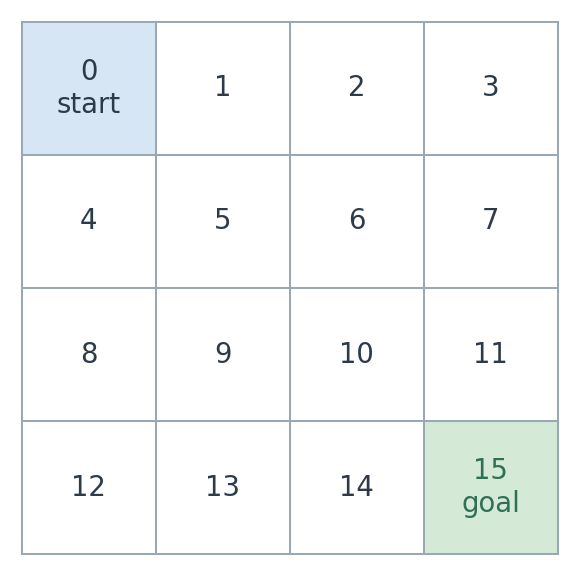
\includegraphics[width=0.42\textwidth]{gridworld_4x4.png}
\caption{GridWorld: start $0$, goal $15$ ($r=0$); every other step $r=-1$. Wall: stay in $s$. Actions: $0$ up, $1$ right, $2$ down, $3$ left.}\label{fig-14-1}
\end{figure}

The GridWorld \textbf{is} an MDP in every case. The four approaches only differ in how they compute $\pi$:

\begin{itemize}
\item \textbf{Value iteration} (dynamic programming) uses $P(s',r\mid s,a)$ and no samples.
\item \textbf{Monte Carlo control} uses samples, with target the finished $G_t$.
\item \textbf{SARSA} uses samples, with one-step target $R+\gamma Q(s',A')$ and $A'\sim\pi$ (on-policy, $Q^\pi$).
\item \textbf{Q-learning} uses samples, with one-step target $R+\gamma\max_{a'}Q(s',a')$ (off-policy, $Q^*$).
\end{itemize}
All four return a greedy $\pi(s)=\arg\max_a Q(s,a)$ (value iteration reads it from $V$). Following that $\pi$ from a start cell is the path.

\lstinputlisting{../code/ch14/gridworld_solutions.py}


VI and Q-learning typically agree on a shortest path to $15$. SARSA can differ on cells where $\varepsilon$-greedy exploration is costly. MC is noisier: its target is a full $G_t$.

\section{Exercise 2: CartPole with DQN}

The task is to \textbf{balance}: keep a pole upright on a cart that rolls on a track. The state is $s = (x, \dot{x}, \varphi, \dot{\varphi}) \in \mathbb{R}^4$: cart position and velocity, pole angle and angular velocity. The pole angle is $\varphi$, not the DQN weights $\theta$. Actions are two horizontal forces on the cart (not on the pole). If the pole is falling one way, the cart must move under it --- the same idea as balancing a stick on a palm.

Here $x$ is the cart's horizontal displacement as the cart rocks back and forth while balancing the pole. The episode ends when $\lvert x\rvert > 2.4$ or $\lvert \varphi \rvert > 12^\circ$, or after $200$ steps. Reward is $1$ every surviving step, so within one episode $G$ rises by $1$ while the pole is up. Across episodes $G$ is not monotone: $\varepsilon$-greedy still falls. $G$ cannot exceed $200$: the episode is cut there even if the pole is still up. A good $\pi$ is a plateau at $200$, not a line that keeps climbing.

The object to learn is $\pi(s)$: which force given $s$. DQN computes $\hat{Q}$, then $\pi(s) = \arg\max_a \hat{Q}(s,a;\theta)$. Acting that $\pi$ every step is how the pole stays up. You do not write a balancing formula by hand.

A table cannot store $Q(s,a)$ for every $s$. The network $\hat{Q}(s,a;\theta)$, replay $\mathcal{D}$, and frozen $\theta^-$ are the DQN update $y = r + \gamma(1-d)\max_{a'} \hat{Q}(s',a';\theta^-)$. SGD on this task is slow; Adam uses the same gradient with an adaptive step. $\varepsilon$ decays as in (6.8).

\begin{figure}[ht]
\centering
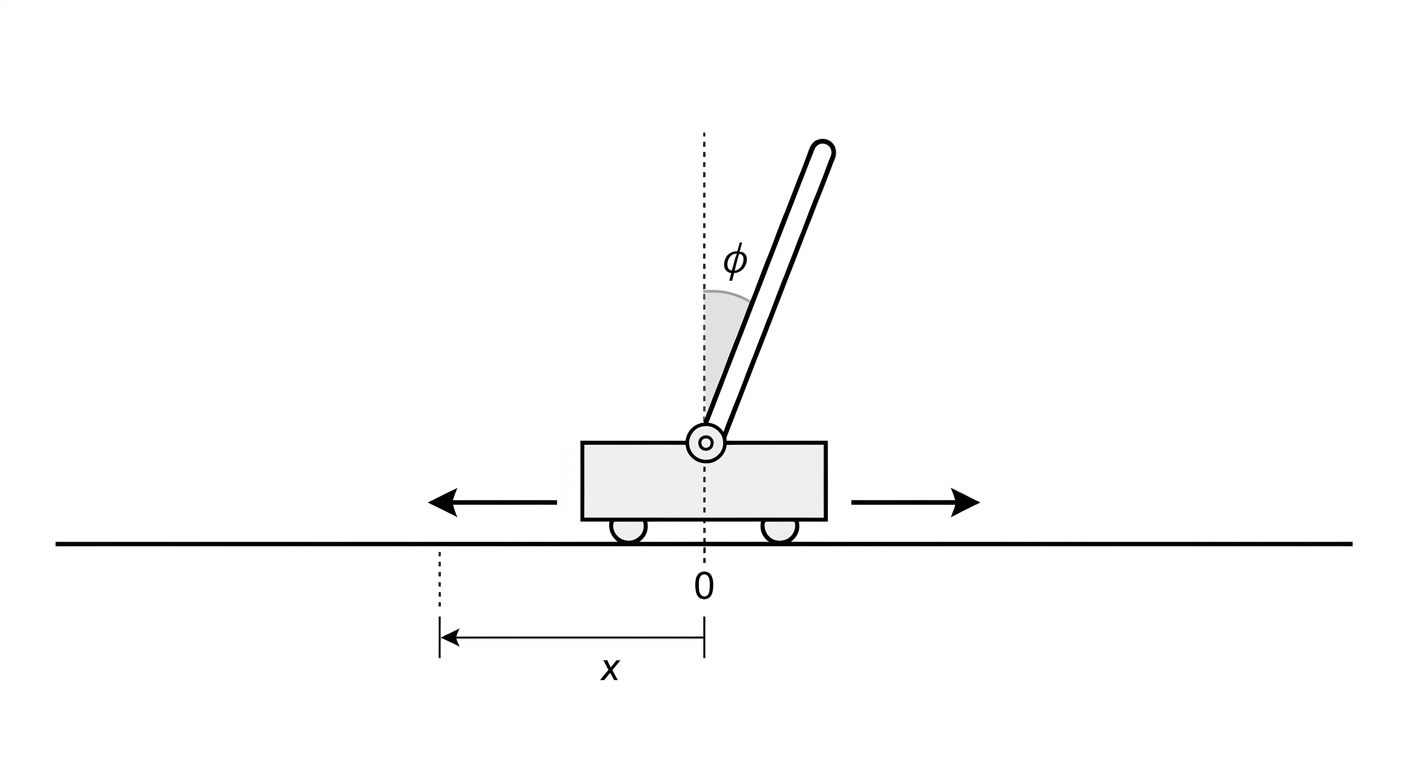
\includegraphics[width=0.72\textwidth]{cartpole.jpeg}
\caption{CartPole balancing task.}
\end{figure}

\lstinputlisting{../code/ch14/cartpole_dqn.py}


\begin{figure}[ht]
\centering
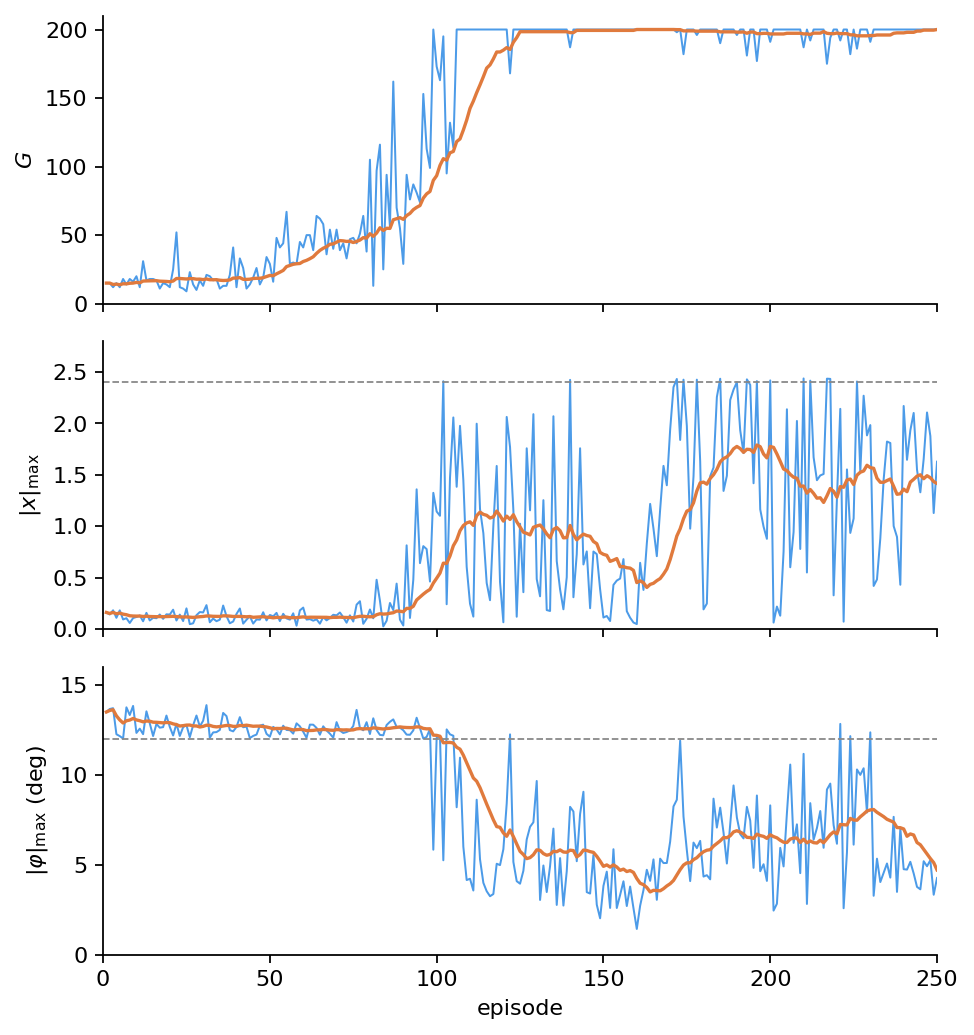
\includegraphics[width=0.72\textwidth,height=0.42\textheight,keepaspectratio]{cartpole_returns.png}
\caption{CartPole DQN, seed $0$: $G$, $|x|_{\max}$, and $|\varphi|_{\max}$ vs episode (blue) and $20$-episode mean (orange). Dashed: fail bounds $2.4$ and $12^\circ$.}\label{fig-14-2}
\end{figure}

Early $G$ near $20$ means the pole (or cart) failed after that many steps. The rise near episode $100$ is balancing starting to work. Orange $G$ flat at $200$ is the step cutoff, not unbounded gain. Late blue dips in $G$ are leftover $\varepsilon$-greedy failures.

Either bound can fail; the other need not. $|\varphi|_{\max}$ above $12^\circ$ with $|x|_{\max}$ still small is a \textbf{pole fall}: the episode stops on $\varphi$, so $x$ never reaches $2.4$. That is the early stretch. $|x|_{\max}$ on $2.4$ with $|\varphi|$ still below $12^\circ$ is a \textbf{cart} fail. The dashed lines are the fail check, not a clip: the failing coordinate can step slightly past the bound, then we stop. After learning, both stay below the dashes for $200$ steps except leftover $\varepsilon$-greedy dips.


\appendix
\chapter{Statistical Concepts}\label{app:A}

The following tools are used in the Bellman derivations that follow, in the Robbins--Monro argument of \appref{D}, and later in off-policy Monte Carlo. Probability relations first, then expectation, then variance, then the law of large numbers, then Monte Carlo estimation, then importance sampling, then the Markov property.

\section{Probability}

\subsection{Law of total probability (LOTP)}

If $B_1,\ldots,B_n$ are mutually exclusive and exhaustive,

\begin{equation}
P(A)
=
\sum_i P(A\mid B_i)\, P(B_i)
=
\sum_i P(A, B_i).
\tag{A.1}
\end{equation}

\section{Expectation}

\subsection{Definition}

For a discrete random variable $X$,

\begin{equation}
\mathbb{E}[X]
=
\sum_x x\, P(X=x).
\tag{A.2}
\end{equation}

\subsection{Conditional expectation}

Conditioning on $Y=y$ (or on an event),

\begin{equation}
\mathbb{E}[X\mid Y=y]
=
\sum_x x\, P(X=x\mid Y=y).
\tag{A.3}
\end{equation}

\subsection{Linearity of (conditional) expectation}

For random variables $Y_1,\ldots,Y_n$ and constants $a_1,\ldots,a_n$,

\begin{equation}
\mathbb{E}[a_1 Y_1+\cdots+a_n Y_n]
=
a_1\mathbb{E}[Y_1]+\cdots+a_n\mathbb{E}[Y_n],
\tag{A.4}
\end{equation}

and conditioning on a random variable $X$ (or on an event):

\begin{equation}
\mathbb{E}[a_1 Y_1+\cdots+a_n Y_n\mid X]
=
a_1\mathbb{E}[Y_1\mid X]+\cdots+a_n\mathbb{E}[Y_n\mid X].
\tag{A.5}
\end{equation}

\textbf{Worked expansion.} For discrete $X_1,X_2$, constants $a,b$, and $Y=y$:

\[
\begin{aligned}
\mathbb{E}[a X_1+b X_2\mid Y=y]
&=
a\,\mathbb{E}[X_1\mid Y=y]
+
b\,\mathbb{E}[X_2\mid Y=y]
\quad\text{[A.5; linearity]}
\\
&=
a\sum_{x_1} x_1\, P(X_1=x_1\mid Y=y)
+
b\sum_{x_2} x_2\, P(X_2=x_2\mid Y=y)
\quad\text{[A.3; conditional expectation]}
\\
&=
a\sum_{x_1} x_1
\sum_{x_2} P(X_1=x_1,X_2=x_2\mid Y=y)
+
b\sum_{x_2} x_2
\sum_{x_1} P(X_1=x_1,X_2=x_2\mid Y=y)
\quad\text{[A.1; LOTP]}
\end{aligned}
\]

\begin{equation}
\mathbb{E}[a X_1+b X_2\mid Y=y]
=
\sum_{x_1,x_2} (a x_1+b x_2)\, P(X_1=x_1,X_2=x_2\mid Y=y).
\tag{A.6}
\end{equation}

(In this book one often takes $a=1$, $b=\gamma$, with $X_1,X_2$ a reward and a return.)

\subsection{Expanding a conditional expectation over a partition}

Start from the definition, then apply LOTP to the conditional probability over the values of a discrete random variable $Y$:

\[
\begin{aligned}
\mathbb{E}[X\mid A]
&=
\sum_x x\, P(X=x\mid A)
\quad\text{[A.3; conditional expectation]}
\\
&=
\sum_x x
\sum_y P(X=x\mid A,Y=y)\, P(Y=y\mid A)
\quad\text{[A.1; LOTP]}
\\
&=
\sum_y
\Bigl(
\sum_x x\, P(X=x\mid A,Y=y)
\Bigr)
P(Y=y\mid A)
\end{aligned}
\]

\begin{equation}
\mathbb{E}[X\mid A]
=
\sum_y \mathbb{E}[X\mid A,Y=y]\, P(Y=y\mid A).
\tag{A.7}
\end{equation}

\subsection{Law of total expectation (tower property)}

Start from the definition of $\mathbb{E}[X]$, expand $P(X=x)$ by LOTP over the values of a discrete $Y$, then regroup:

\[
\begin{aligned}
\mathbb{E}[X]
&=
\sum_x x\, P(X=x)
\quad\text{[A.2]}
\\
&=
\sum_x x
\sum_y P(X=x\mid Y=y)\, P(Y=y)
\quad\text{[A.1; LOTP]}
\\
&=
\sum_y
\Bigl(
\sum_x x\, P(X=x\mid Y=y)
\Bigr)
P(Y=y)
\\
&=
\sum_y \mathbb{E}[X\mid Y=y]\, P(Y=y)
\quad\text{[A.3]}
\\
&=
\mathbb{E}\bigl[\mathbb{E}[X\mid Y]\bigr].
\end{aligned}
\]

So

\begin{equation}
\mathbb{E}[X]
=
\mathbb{E}\bigl[\mathbb{E}[X\mid Y]\bigr].
\tag{A.8}
\end{equation}

The same argument with the event $\{Z=z\}$ in place of the unconditional law gives the conditional tower. Apply (A.7) with $A=\{Z=z\}$ and partition by $Y$:

\[
\begin{aligned}
\mathbb{E}[X\mid Z=z]
&=
\sum_y \mathbb{E}[X\mid Z=z,Y=y]\, P(Y=y\mid Z=z)
\quad\text{[A.7]}
\\
&=
\sum_y \mathbb{E}[X\mid Y=y,Z=z]\, P(Y=y\mid Z=z).
\end{aligned}
\]

For each fixed pair $(y,z)$, the number $\mathbb{E}[X\mid Y=y,Z=z]$ depends only on those values. Collecting them into a random variable that is a \textbf{function of $(Y,Z)$},

\[
g(Y,Z)
:=
\mathbb{E}[X\mid Y,Z],
\]

the sum above is the conditional expectation of that function given $Z=z$:

\[
\begin{aligned}
\mathbb{E}[X\mid Z=z]
&=
\sum_y g(y,z)\, P(Y=y\mid Z=z)
\\
&=
\mathbb{E}\bigl[g(Y,Z)\bigm|\ Z=z\bigr]
\\
&=
\mathbb{E}\bigl[\mathbb{E}[X\mid Y,Z]\bigm|\ Z=z\bigr].
\end{aligned}
\]

Writing the same identity for every $z$ as a random-variable equation:

\begin{equation}
\mathbb{E}[X\mid Z]
=
\mathbb{E}\bigl[\mathbb{E}[X\mid Y,Z]\bigm|\ Z\bigr].
\tag{A.9}
\end{equation}

In discrete form with $Y$ taking values $y$ (the expansion used above):

\begin{equation}
\mathbb{E}[X\mid Z=z]
=
\sum_y \mathbb{E}[X\mid Y=y,Z=z]\, P(Y=y\mid Z=z).
\tag{A.10}
\end{equation}

So (A.10) is (A.9) written pointwise at $Z=z$; (A.8) is the special case of (A.9) with no conditioning on $Z$ (or with $Z$ trivial).

\subsection{Expectation of a function of a discrete random variable (Law of the Unconscious Statistician)}

The identity $\mathbb{E}[f(X)]=\sum_x f(x)\,P(X=x)$ is also called the \textbf{law of the unconscious statistician (LOTUS)}, or sometimes the \textbf{law of the lazy statistician}: one need not first find the distribution of $Y=f(X)$; the expectation follows from the distribution of $X$ alone.

Let $X$ be discrete and set $Y=f(X)$. Then $P(Y=y)$ is the sum of all probabilities of those $x$ for which $f(x)=y$:

\[
P(Y=y)
=
\sum_{x:\,f(x)=y} P(X=x).
\quad\text{[A.1; LOTP]}
\]

Then

\begin{equation}
\begin{aligned}
\mathbb{E}[f(X)]
&=
\mathbb{E}[Y]
=
\sum_y y\, P(Y=y)
\\
&=
\sum_y y
\left(
\sum_{x:\,f(x)=y} P(X=x)
\right)
\\
&=
\sum_y
\left(
\sum_{x:\,f(x)=y} y\, P(X=x)
\right)
\\
&=
\sum_y
\left(
\sum_{x:\,f(x)=y} f(x)\, P(X=x)
\right)
\quad\text{[$y=f(x)$ on each inner sum]}
\\
&=
\sum_x f(x)\, P(X=x).
\end{aligned}
\tag{A.12}
\end{equation}

The last equality collapses the nested sums. For each fixed $y$, the inner sum runs only over the group $\{x:f(x)=y\}$: any $x$ with $f(x)\neq y$ is missing from that group. Because $f$ is a function, every $x$ maps to exactly one $y$, so each $x$ appears in \textbf{exactly one} group, and every $x$ appears in \textbf{some} group. Summing $f(x)\,P(X=x)$ group by group is therefore the same as summing once over all $x$.

\textbf{Example.} Suppose the possible values of $X$ are $\{1,2,3\}$ and $f(1)=f(2)=a$, $f(3)=b$. The double sum is two groups:

\[
\sum_{x:\,f(x)=a} f(x)\,P(X=x)
+
\sum_{x:\,f(x)=b} f(x)\,P(X=x)
=
\bigl(f(1)P(X=1)+f(2)P(X=2)\bigr)
+
f(3)P(X=3),
\]

which is exactly $\sum_{x\in\{1,2,3\}} f(x)\,P(X=x)$. In the $a$-group, $x=3$ is missing; in the $b$-group, $x=1$ and $x=2$ are missing; no $x$ appears in both.

(The same steps with $P(\,\cdot\mid A)$ give $\mathbb{E}[f(X)\mid A]=\sum_x f(x)\,P(X=x\mid A)$.)

\subsection{Variance and standard deviation}

Write $\mu=\mathbb{E}[X]$. The \textbf{variance} is the expected squared deviation from that mean,

\begin{equation}
\mathrm{Var}(X)
=
\mathbb{E}\bigl[(X-\mu)^2\bigr].
\tag{A.17}\label{eq:A.17}
\end{equation}

The \textbf{standard deviation} is the positive square root,

\begin{equation}
\sigma_X
=
\sqrt{\mathrm{Var}(X)}.
\tag{A.18}\label{eq:A.18}
\end{equation}

So $\mathrm{Var}(X)=\sigma_X^2$. Expanding the square in (A.17) and using linearity (A.5) with $\mathbb{E}[X]=\mu$ gives the computational form

\begin{equation}
\mathrm{Var}(X)
=
\mathbb{E}[X^2]-(\mathbb{E}[X])^2.
\tag{A.19}\label{eq:A.19}
\end{equation}

If $\mathbb{E}[X]=0$, then (A.19) is $\mathrm{Var}(X)=\mathbb{E}[X^2]$. For a finite list $x_1,\ldots,x_n$ with list mean $\bar x$, the same square-root of mean squared deviation from $\bar x$ is written $\mathrm{std}$.

\section{Law of large numbers}\label{app:A.3}

The \textbf{weak law of large numbers} says: if $x_1,\ldots,x_n$ are i.i.d.\ samples from the distribution of a random variable $X$ with expectation $\mu=\mathbb{E}[X]$ and finite variance $\mathrm{Var}(X)=\sigma_X^2$, as in (A.17)--(A.18), then the sample mean of those draws has expectation $\mu$ and converges to $\mu$. Write the sample mean as
\begin{equation}
\bar{x}_n
=
\frac{1}{n}\sum_{i=1}^{n} x_i.
\tag{A.20}\label{eq:A.20}
\end{equation}
Then $\mathbb{E}[\bar{x}_n]=\mu$, and $\bar{x}_n\to\mu$ in probability as $n\to\infty$.

\textbf{Proof.}

Linearity (A.4) gives
\begin{equation}
\mathbb{E}[\bar{x}_n]
=
\frac{1}{n}\sum_{i=1}^{n} \mathbb{E}[x_i]
=
\mu.
\tag{A.21}\label{eq:A.21}
\end{equation}
So $\bar{x}_n$ is unbiased for $\mu$.

For a constant $a$, (A.17) gives $\mathrm{Var}(aX)=a^2\mathrm{Var}(X)$. For independent $X$ and $Y$,
\[
\begin{aligned}
\mathrm{Var}(X+Y)
&=
\mathbb{E}\bigl[((X-\mu_X)+(Y-\mu_Y))^2\bigr]
\\
&=
\mathrm{Var}(X)+\mathrm{Var}(Y)+2\,\mathbb{E}[(X-\mu_X)(Y-\mu_Y)].
\end{aligned}
\]
Independence factors the cross term:
\[
\mathbb{E}[(X-\mu_X)(Y-\mu_Y)]
=
\mathbb{E}[X-\mu_X]\,\mathbb{E}[Y-\mu_Y].
\]
Each factor is the expectation of a deviation from the mean, so
\[
\mathbb{E}[X-\mu_X]
=
\mathbb{E}[X]-\mu_X
=
\mu_X-\mu_X
=
0,
\]
and likewise $\mathbb{E}[Y-\mu_Y]=\mathbb{E}[Y]-\mu_Y=\mu_Y-\mu_Y=0$. The product is therefore $0$, and
\[
\mathrm{Var}(X+Y)=\mathrm{Var}(X)+\mathrm{Var}(Y).
\]
Repeating for $n$ i.i.d.\ samples,
\begin{equation}
\mathrm{Var}(\bar{x}_n)
=
\mathrm{Var}\!\left(\frac{1}{n}\sum_{i=1}^{n} x_i\right)
=
\frac{1}{n^2}\sum_{i=1}^{n} \mathrm{Var}(x_i)
=
\frac{\sigma_X^2}{n}.
\tag{A.22}\label{eq:A.22}
\end{equation}
The standard deviation of $\bar{x}_n$ is $\sigma_X/\sqrt{n}$. As $n\to\infty$, that variance goes to $0$. Chebyshev's inequality bounds how far a random variable can sit from its mean: for a random variable $Y$ with mean $\nu$ and finite variance, and every $\varepsilon>0$,
\[
P\bigl(|Y-\nu|\ge\varepsilon\bigr)
\le
\frac{\mathrm{Var}(Y)}{\varepsilon^2}.
\]
Taking $Y=\bar{x}_n$ and $\nu=\mu$ with (A.22) gives
\begin{equation}
P\bigl(|\bar{x}_n-\mu|\ge\varepsilon\bigr)
\le
\frac{\mathrm{Var}(\bar{x}_n)}{\varepsilon^2}
=
\frac{\sigma_X^2}{n\varepsilon^2}
\to 0.
\tag{A.23}\label{eq:A.23}
\end{equation}
So $\bar{x}_n\to\mu$ in probability, which is the claim at the start of this section. The same Chebyshev bound is used in \appref{D}.

\section{Monte Carlo estimation}\label{app:A.4}

\textbf{Monte Carlo} estimates an expectation $\mathbb{E}[f(X)]$ by drawing i.i.d.\ samples $x_1,\ldots,x_n$ from the distribution of $X$ and averaging the observed values of $f$. The estimator is
\begin{equation}
\bar{f}_n
=
\frac{1}{n}\sum_{i=1}^{n} f(x_i).
\tag{A.24}\label{eq:A.24}
\end{equation}
If $\mathrm{Var}(f(X))$ is finite, then $\mathbb{E}[\bar{f}_n]=\mathbb{E}[f(X)]$, and $\bar{f}_n\to\mathbb{E}[f(X)]$ in probability as $n\to\infty$. Chapter 4 uses it with $f$ the return $G_t$ from a visit to $s$.

\textbf{Proof.}
Replace each $x_i$ in (A.20) by $f(x_i)$, which is legitimate by (A.12). Then (A.21)--(A.23) apply with $X$ replaced by $f(X)$, so $\bar{f}_n$ is unbiased for $\mathbb{E}[f(X)]$ and converges to it.

\section{Importance sampling}

Importance sampling estimates an expectation under a target $p$ from samples drawn under a proposal $q$, by reweighting each sample with $w=p/q$. Example: estimate mean height in the population ($p$) from players at a basketball camp ($q$); tall players are common at camp but rare in the population, so $w$ downweights them.

Expectation is still (A.2): $\mathbb{E}[Y]=\sum_y y\,P(Y=y)$. When $Y=f(X)$ and $X$ has distribution $p$, (A.12) writes that as a sum over $x$: \[
\mathbb{E}_{x\sim p}[f(x)]
=
\sum_x f(x)\, p(x)
\]

(for discrete $x$; continuous cases replace the sum by an integral). If we could draw $x_1,\ldots,x_N$ from $p$, the Monte Carlo average (A.24) of the values $f(x_i)$ would estimate that expectation.

Often we \textbf{cannot} (or do not) sample from $p$. Instead we have samples from a different distribution $q$ (the \textbf{proposal} or \textbf{behavior} distribution), with $q(x)>0$ whenever $p(x)>0$ and $f(x)\neq 0$. A plain average under $q$ estimates $\mathbb{E}_{x\sim q}[f(x)]$, which is the wrong target. Importance sampling rewrites the $p$-expectation as a $q$-expectation by inserting the ratio $p/q$: \begin{equation}
\begin{aligned}
\mathbb{E}_{x\sim p}[f(x)]
&=
\sum_x f(x)\, p(x)
\\
&=
\sum_x f(x)\, \frac{p(x)}{q(x)}\, q(x)
\\
&=
\sum_x w(x)\, f(x)\, q(x)
\\
&=
\mathbb{E}_{x\sim q}\bigl[w(x)\, f(x)\bigr],
\qquad
w(x)=\frac{p(x)}{q(x)}.
\end{aligned}
\tag{A.13}\label{eq:A.13}
\end{equation}

The weight has mean one under $q$:

\[
\begin{aligned}
\mathbb{E}_{x\sim q}[w(x)]
&=
\sum_x w(x)\, q(x)
\\
&=
\sum_x \frac{p(x)}{q(x)}\, q(x)
\\
&=
\sum_x p(x)
\\
&=
1.
\end{aligned}
\]

Dividing the right-hand side of (A.13) by this identity,

\begin{equation}
\begin{aligned}
\mathbb{E}_{x\sim p}[f(x)]
&=
\mathbb{E}_{x\sim q}\bigl[w(x)\, f(x)\bigr]
\\
&=
\frac{\mathbb{E}_{x\sim q}\bigl[w(x)\, f(x)\bigr]}{\mathbb{E}_{x\sim q}[w(x)]}.
\end{aligned}
\tag{A.14}
\end{equation}

With i.i.d. samples $x_i\sim q$, estimate the expectations by sample means. Estimating only the numerator of (A.14) (equivalently, the last line of (A.13)) gives \textbf{ordinary} importance sampling:

\begin{equation}
\mathbb{E}_{x\sim p}[f(x)]
\approx
\frac{1}{N}\sum_{i=1}^{N} w(x_i)\, f(x_i).
\tag{A.15}
\end{equation}

Estimating both the numerator and the denominator of (A.14) gives \textbf{weighted} (self-normalized) importance sampling:

\begin{equation}
\mathbb{E}_{x\sim p}[f(x)]
\approx
\frac{\tfrac{1}{N}\sum_{i=1}^{N} w(x_i)\, f(x_i)}
{\tfrac{1}{N}\sum_{i=1}^{N} w(x_i)}
=
\frac{\sum_{i=1}^{N} w(x_i)\, f(x_i)}{\sum_{i=1}^{N} w(x_i)}.
\tag{A.16}
\end{equation}

A single term $w(x)\,f(x)$ is already an \textbf{unbiased} estimator of $\mathbb{E}_p[f]$, since its mean equals $\mathbb{E}_p[f]$ by (A.13). Ordinary importance sampling (A.15) averages $N$ such terms, so it is unbiased for $\mathbb{E}_p[f]$ as well. Weighted importance sampling (A.16) estimates the same target but is \textbf{biased} for finite $N$. It divides two random averages built from the same samples, and the mean of a ratio need not equal the ratio of the means. That bias goes away as $N$ grows. The cost of ordinary IS shows up in variance. If a few samples carry large weights and many carry small ones, (A.15) is driven by those few terms and can jump a lot from one run to the next. Weighted (A.16) is usually stabler. A large $w$ increases both the numerator and the denominator, so no single sample can take more than its share of the total weight.

If $q$ oversamples a region relative to $p$, then $w<1$ there (downweight); if $q$ undersamples it, then $w>1$ (upweight). Importance sampling \textbf{reweights} every draw. Rejection sampling instead \textbf{accepts or drops}; that procedure, and the hard-filter case, is \appref{H}.

\section{Markov property}

Given $S_{t+1}=s'$, the remaining return $G_{t+1}$ does not depend on $(S_t,A_t)$:

\begin{equation}
\mathbb{E}_\pi[G_{t+1}\mid S_t=s,A_t=a,S_{t+1}=s']
=
\mathbb{E}_\pi[G_{t+1}\mid S_{t+1}=s'].
\tag{A.11}
\end{equation}

\chapter{Bellman Expectation Derivation}\label{app:B}

\section*{Goal}

Derive the Bellman expectation equations for a fixed policy $\pi$, and also the policy-averaged form of $V^\pi$ used in matrix policy evaluation.

\begin{equation}
V^\pi(s)
=
\sum_{a}
\pi(a \mid s)
\sum_{s',r}
P(s',r \mid s,a)
\left[
r + \gamma V^\pi(s')
\right].
\tag{B.1}\label{eq:B.1}
\end{equation}

\begin{equation}
Q^\pi(s,a)
=
\sum_{s',r}
P(s',r \mid s,a)
\left[
r + \gamma \sum_{a'} \pi(a' \mid s') Q^\pi(s',a')
\right].
\tag{B.2}\label{eq:B.2}
\end{equation}

\begin{equation}
V^\pi(s)
=
R^\pi(s)
+
\gamma
\sum_{s'}
P^\pi(s' \mid s)\, V^\pi(s').
\tag{B.3}\label{eq:B.3}
\end{equation}

B.3 derives (B.1) and (B.3), with compact form (B.11). B.4 derives (B.2), with compact form (B.18). B.5 collects the expectation links between $V^\pi$ and $Q^\pi$ used in later chapters. Expected rewards $R(s,a,s')$, $R(s,a)$, and $R^\pi(s)$ are (B.4), (B.5), and (B.12).

\section{Expected rewards}

\[
R(s,a,s')=\mathbb{E}[R_{t+1}\mid S_t=s,A_t=a,S_{t+1}=s'];
\quad\text{expected reward from taking $a$ in $s$ and arriving at $s'$}.
\]

\[
\begin{aligned}
R(s,a,s')
&=
\sum_r r\, P(R_{t+1}=r\mid S_t=s,A_t=a,S_{t+1}=s')
\quad\text{[A.3; conditional expectation]}
\\
&=
\sum_r r\, \frac{P(s',r\mid s,a)}{P(s'\mid s,a)}
\quad\text{[conditional probability]}.
\end{aligned}
\]

\begin{equation}
R(s,a,s')
=
\sum_r r\, \frac{P(s',r\mid s,a)}{P(s'\mid s,a)}.
\tag{B.4}\label{eq:B.4}
\end{equation}

\[
R(s,a)=\mathbb{E}[R_{t+1}\mid S_t=s,A_t=a];
\quad\text{expected reward from taking $a$ in $s$}.
\]

Expand over the next state by (A.7), then substitute (B.4):

\[
\begin{aligned}
R(s,a)
&=
\sum_{s'}
\mathbb{E}[R_{t+1}\mid S_t=s,A_t=a,S_{t+1}=s']
\,
P(s'\mid s,a)
\quad\text{[A.7; partition expansion]}
\\
&=
\sum_{s'}
R(s,a,s')\, P(s'\mid s,a)
\\
&=
\sum_{s'}
\Bigl(
\sum_r r\, \frac{P(s',r\mid s,a)}{P(s'\mid s,a)}
\Bigr)
P(s'\mid s,a)
\quad\text{[(B.4)]}
\\
&=
\sum_{s',r} r\, P(s',r\mid s,a).
\end{aligned}
\]

\begin{equation}
R(s,a)
=
\sum_{s',r} r\, P(s',r\mid s,a)
=
\sum_{s'} P(s'\mid s,a)\, R(s,a,s').
\tag{B.5}\label{eq:B.5}
\end{equation}

\section{Trajectory and environment dynamics}

To model how an agent interacts with its environment over time, consider a sequential trajectory in a Markov Decision Process (MDP):

\[
S_t \xrightarrow{A_t} (S_{t+1}, R_{t+1}) \xrightarrow{A_{t+1}} (S_{t+2}, R_{t+2}) \xrightarrow{A_{t+2}} \dots
\]

\begin{enumerate}
\item \textbf{State $S_t = s$}: The agent starts at time step $t$ in state $s$.
\item \textbf{Action $A_t = a$}: The probability of selecting action $A_t = a$ in state $S_t = s$ is $P(A_t = a \mid S_t = s)$, also called the policy and written as $\pi(a \mid s)$.
\item \textbf{Transition \& Reward $(S_{t+1} = s', R_{t+1} = r)$}: Given state $S_t = s$ and action $A_t = a$, the environment transitions to next state $S_{t+1} = s'$ and gives reward $R_{t+1} = r$ with joint probability $P(s', r \mid s, a) = P(S_{t+1} = s', R_{t+1} = r \mid S_t = s, A_t = a)$. \textit{Note: Due to environmental stochasticity, both state transitions and reward outcomes are probabilistic; even when transitioning from state $s$ to the exact same next state $s'$ via action $a$, the immediate reward $R_{t+1}$ can vary according to this distribution.}
\end{enumerate}

\subsection{Return $G_t$}

The total discounted return $G_t$ from step $t$ is the sum of all future rewards:

\begin{equation}
G_t = R_{t+1} + \gamma R_{t+2} + \gamma^2 R_{t+3} + \dots = R_{t+1} + \gamma G_{t+1}
\tag{B.6}
\end{equation}

where $R_{t+1}$ is the immediate reward and $\gamma \in [0, 1]$ is the discount factor.

\section{State-value $V^\pi$}

We want (B.1).

\subsection{Define the state-value function}

\begin{equation}
V^\pi(s)
=
\mathbb{E}_\pi[G_t\mid S_t=s]
\tag{B.7}
\end{equation}

\subsection{Substitute the recursive return}

From (B.6), $G_t=R_{t+1}+\gamma G_{t+1}$. Therefore,

\begin{equation}
\begin{aligned}
V^\pi(s)
&=
\mathbb{E}_\pi[G_t\mid S_t=s] \\
&=
\mathbb{E}_\pi[R_{t+1}+\gamma G_{t+1}\mid S_t=s] \\
&=
\mathbb{E}_\pi[R_{t+1}\mid S_t=s]
+
\gamma\mathbb{E}_\pi[G_{t+1}\mid S_t=s]
\end{aligned}
\tag{B.8}
\end{equation}

We derive the two terms separately.

\subsection{Immediate Reward}

Expand over $A_t$ by (A.7). Each inner expectation is the definition (A.3), then LOTP (A.1) writes the joint $P(s',r\mid s,a)$:

\[
\begin{aligned}
\mathbb{E}_\pi[R_{t+1}\mid S_t=s]
&=
\sum_a
\mathbb{E}[R_{t+1}\mid S_t=s,A_t=a]
\,
\pi(a\mid s)
\quad\text{[A.7; partition expansion]}
\\
&=
\sum_a\pi(a\mid s)
\sum_r r\,
P(R_{t+1}=r\mid S_t=s,A_t=a)
\quad\text{[A.3; conditional expectation]}
\\
&=
\sum_a\pi(a\mid s)
\sum_{s',r}
r\, P(s',r\mid s,a)
\quad\text{[A.1; LOTP]}.
\end{aligned}
\]

\begin{equation}
\boxed{
\mathbb{E}_\pi[R_{t+1}\mid S_t=s]
=
\sum_a\pi(a\mid s)
\sum_{s',r}
rP(s',r\mid s,a)
}
\tag{B.9}
\end{equation}

\subsection{Future Return}

Expand over $A_t$, then over $S_{t+1}$, by (A.7). Markov (A.11) drops $(s,a)$ given $s'$; the inner expectation is $V^\pi(s')$ by (B.7). A last LOTP writes $P(s'\mid s,a)=\sum_r P(s',r\mid s,a)$:

\[
\begin{aligned}
\mathbb{E}_\pi[G_{t+1}\mid S_t=s]
&=
\sum_a
\mathbb{E}_\pi[G_{t+1}\mid S_t=s,A_t=a]
\,
\pi(a\mid s)
\quad\text{[A.7; partition expansion]}
\\
&=
\sum_a\pi(a\mid s)
\sum_{s'}
\mathbb{E}_\pi[G_{t+1}\mid S_t=s,A_t=a,S_{t+1}=s']
\,
P(s'\mid s,a)
\quad\text{[A.7; partition expansion]}
\\
&=
\sum_a\pi(a\mid s)
\sum_{s'}
\mathbb{E}_\pi[G_{t+1}\mid S_{t+1}=s']
\,
P(s'\mid s,a)
\quad\text{[A.11; Markov]}
\\
&=
\sum_a\pi(a\mid s)
\sum_{s'}
V^\pi(s')\, P(s'\mid s,a)
\quad\text{[(B.7)]}
\\
&=
\sum_a\pi(a\mid s)
\sum_{s',r}
P(s',r\mid s,a)\, V^\pi(s')
\quad\text{[A.1; LOTP]}.
\end{aligned}
\]

\begin{equation}
\boxed{
\mathbb{E}_\pi[G_{t+1}\mid S_t=s]
=
\sum_a
\pi(a\mid s)
\sum_{s',r}
P(s',r\mid s,a)V^\pi(s')
}
\tag{B.10}
\end{equation}

\subsection{Combine}

Recall (B.8). Substitute (B.9) and (B.10):

\[
\begin{aligned}
V^\pi(s)
&=
\sum_a\pi(a\mid s)
\sum_{s',r}
rP(s',r\mid s,a)
\\
&\qquad+
\gamma
\sum_a\pi(a\mid s)
\sum_{s',r}
P(s',r\mid s,a)V^\pi(s')
\end{aligned}
\]

Factor the common terms:

\begin{equation}
\boxed{
V^\pi(s)
=
\sum_a
\pi(a\mid s)
\sum_{s',r}
P(s',r\mid s,a)
\left[
r+\gamma V^\pi(s')
\right]
}
\tag{B.1}
\end{equation}

This is the \textbf{Bellman Expectation Equation} (B.1).

\subsection{Compact one-step form}

Start from (B.8):

\[
V^\pi(s)
=
\mathbb{E}_\pi[R_{t+1}\mid S_t=s]
+
\gamma
\mathbb{E}_\pi[G_{t+1}\mid S_t=s].
\]

For the future term, apply the tower property (A.9) with $X=G_{t+1}$, $Y=S_{t+1}$, and $Z=S_t$. The inner conditional expectation is a function of $(S_{t+1},S_t)$:

\[
\mathbb{E}_\pi[G_{t+1}\mid S_t]
=
\mathbb{E}_\pi\bigl[
\mathbb{E}_\pi[G_{t+1}\mid S_{t+1},S_t]
\bigm|
S_t
\bigr]
\quad\text{[A.9]}.
\]

Given $S_{t+1}$, the Markov property (A.11) drops $S_t$, and the inner expectation is $V^\pi(S_{t+1})$ by (B.7):

\[
\begin{aligned}
\mathbb{E}_\pi[G_{t+1}\mid S_{t+1},S_t]
&=
\mathbb{E}_\pi[G_{t+1}\mid S_{t+1}]
\quad\text{[A.11; Markov]}
\\
&=
V^\pi(S_{t+1})
\quad\text{[(B.7)]}.
\end{aligned}
\]

Therefore

\[
\mathbb{E}_\pi[G_{t+1}\mid S_t]
=
\mathbb{E}_\pi\bigl[V^\pi(S_{t+1})\mid S_t\bigr],
\]

and evaluating at $S_t=s$,

\[
\mathbb{E}_\pi[G_{t+1}\mid S_t=s]
=
\mathbb{E}_\pi\bigl[V^\pi(S_{t+1})\mid S_t=s\bigr].
\]

Substitute back into (B.8) and apply linearity (A.5):

\[
\begin{aligned}
V^\pi(s)
&=
\mathbb{E}_\pi[R_{t+1}\mid S_t=s]
+
\gamma
\mathbb{E}_\pi\bigl[V^\pi(S_{t+1})\mid S_t=s\bigr]
\\
&=
\mathbb{E}_\pi\bigl[R_{t+1}+\gamma V^\pi(S_{t+1})\mid S_t=s\bigr]
\quad\text{[A.5; linearity]}.
\end{aligned}
\]

\begin{equation}
\boxed{
V^\pi(s)
=
\mathbb{E}_\pi\bigl[R_{t+1}+\gamma V^\pi(S_{t+1})\mid S_t=s\bigr].
}
\tag{B.11}\label{eq:B.11}
\end{equation}

\textbf{Alternative derivation (discrete expansion).} The same identity for $\mathbb{E}_\pi[G_{t+1}\mid S_t=s]$ can be written by expanding over next-state values with (A.10), then applying Markov and (B.7):

\[
\begin{aligned}
\mathbb{E}_\pi[G_{t+1}\mid S_t=s]
&=
\sum_{s'}
\mathbb{E}_\pi[G_{t+1}\mid S_t=s,S_{t+1}=s']
\,
P_\pi(S_{t+1}=s'\mid S_t=s)
\quad\text{[A.10]}
\\
&=
\sum_{s'}
\mathbb{E}_\pi[G_{t+1}\mid S_{t+1}=s']
\,
P_\pi(S_{t+1}=s'\mid S_t=s)
\quad\text{[A.11; Markov]}
\\
&=
\sum_{s'}
V^\pi(s')
\,
P_\pi(S_{t+1}=s'\mid S_t=s)
\quad\text{[(B.7)]}
\\
&=
\mathbb{E}_\pi\bigl[V^\pi(S_{t+1})\mid S_t=s\bigr].
\end{aligned}
\]

Substituting into (B.8) and using linearity (A.5) recovers (B.11) as before.

\subsection{Policy-averaged form}

\textbf{Why ``policy-averaged''.} The one-step quantities $R(s,a)$ and $P(s'\mid s,a)$ still depend on the chosen action. Averaging them with weights $\pi(a\mid s)$ produces state-only objects $R^\pi(s)$ and $P^\pi(s'\mid s)$---the reward and transition \textbf{averaged under the policy}. Equation (B.1) writes those averages out explicitly; the form below absorbs them into $R^\pi$ and $P^\pi$, which is what matrix policy evaluation uses.

Define $R^\pi(s)=\mathbb{E}_\pi[R_{t+1}\mid S_t=s]$: the expected immediate reward from $s$ when actions are chosen by $\pi$. Expand over $A_t$ by (A.7) and use (B.5):

\[
\begin{aligned}
R^\pi(s)
&=
\sum_a
\mathbb{E}[R_{t+1}\mid S_t=s,A_t=a]
\,
\pi(a\mid s)
\quad\text{[A.7; partition expansion]}
\\
&=
\sum_a\pi(a\mid s)\, R(s,a)
\quad\text{[(B.5)]}.
\end{aligned}
\]

\begin{equation}
R^\pi(s)
=
\sum_a\pi(a\mid s)\, R(s,a).
\tag{B.12}\label{eq:B.12}
\end{equation}

Define $P^\pi(s'\mid s)=P_\pi(S_{t+1}=s'\mid S_t=s)$: the probability of moving from $s$ to $s'$ under $\pi$. By (A.1),

\[
P^\pi(s'\mid s)
=
\sum_a\pi(a\mid s)\, P(s'\mid s,a).
\]

Start from the compact form (B.11). Apply linearity (A.5), then write the two expectations with (B.12) and the definition of $P^\pi$:

\[
\begin{aligned}
V^\pi(s)
&=
\mathbb{E}_\pi\bigl[R_{t+1}+\gamma V^\pi(S_{t+1})\mid S_t=s\bigr]
\quad\text{[(B.11)]}
\\
&=
\mathbb{E}_\pi[R_{t+1}\mid S_t=s]
+
\gamma
\mathbb{E}_\pi\bigl[V^\pi(S_{t+1})\mid S_t=s\bigr]
\quad\text{[A.5; linearity]}
\\
&=
R^\pi(s)
+
\gamma
\sum_{s'}
V^\pi(s')\, P^\pi(s'\mid s)
\quad\text{[(B.12); definition of $P^\pi$]}.
\end{aligned}
\]

\begin{equation}
\boxed{
V^\pi(s)
=
R^\pi(s)
+
\gamma
\sum_{s'}
P^\pi(s'\mid s)\, V^\pi(s')
}
\tag{B.3}
\end{equation}

\section{Action-value $Q^\pi$}

We want (B.2). An intermediate step is (B.17).

\subsection{Define the action-value function}

\begin{equation}
Q^\pi(s,a)
=
\mathbb{E}_\pi[G_t\mid S_t=s,A_t=a]
\tag{B.13}
\end{equation}

\subsection{Relate $V^\pi(s)$ to $Q^\pi(s,a)$}

Expand over $A_t$ by (A.7). The inner expectation is $Q^\pi(s,a)$ by (B.13):

\[
\begin{aligned}
V^\pi(s)
&=
\mathbb{E}_\pi[G_t\mid S_t=s]
\quad\text{[(B.7)]}
\\
&=
\sum_a
\mathbb{E}_\pi[G_t\mid S_t=s,A_t=a]
\,
\pi(a\mid s)
\quad\text{[A.7; partition expansion]}
\\
&=
\sum_a\pi(a\mid s)\, Q^\pi(s,a)
\quad\text{[(B.13)]}.
\end{aligned}
\]

\begin{equation}
\boxed{
V^\pi(s)
=
\sum_a \pi(a\mid s)\, Q^\pi(s,a)
}
\tag{B.14}\label{eq:B.14}
\end{equation}

\subsection{Substitute the recursive return}

From (B.6), $G_t=R_{t+1}+\gamma G_{t+1}$. Therefore,

\[
\begin{aligned}
Q^\pi(s,a)
&=
\mathbb{E}_\pi[G_t\mid S_t=s,A_t=a] \\
&=
\mathbb{E}_\pi[R_{t+1}+\gamma G_{t+1}\mid S_t=s,A_t=a] \\
&=
\mathbb{E}_\pi[R_{t+1}\mid S_t=s,A_t=a]
+
\gamma
\mathbb{E}_\pi[G_{t+1}\mid S_t=s,A_t=a].
\end{aligned}
\]

We derive the two terms separately.

\subsection{Immediate Reward}

The action is already fixed. Apply the definition (A.3), then LOTP (A.1) for the joint $P(s',r\mid s,a)$:

\[
\begin{aligned}
\mathbb{E}_\pi[R_{t+1}\mid S_t=s,A_t=a]
&=
\sum_r r\,
P(R_{t+1}=r\mid S_t=s,A_t=a)
\quad\text{[A.3; conditional expectation]}
\\
&=
\sum_{s',r}
r\, P(s',r\mid s,a)
\quad\text{[A.1; LOTP]}.
\end{aligned}
\]

\begin{equation}
\boxed{
\mathbb{E}_\pi[R_{t+1}\mid S_t=s,A_t=a]
=
\sum_{s',r}
rP(s',r\mid s,a)
}
\tag{B.15}
\end{equation}

\subsection{Future Return}

Expand over $S_{t+1}$ by (A.7). Markov (A.11) drops $(s,a)$ given $s'$; the inner expectation is $V^\pi(s')$ by (B.7). A last LOTP writes $P(s'\mid s,a)=\sum_r P(s',r\mid s,a)$:

\[
\begin{aligned}
\mathbb{E}_\pi[G_{t+1}\mid S_t=s,A_t=a]
&=
\sum_{s'}
\mathbb{E}_\pi[G_{t+1}\mid S_t=s,A_t=a,S_{t+1}=s']
\,
P(s'\mid s,a)
\quad\text{[A.7; partition expansion]}
\\
&=
\sum_{s'}
\mathbb{E}_\pi[G_{t+1}\mid S_{t+1}=s']
\,
P(s'\mid s,a)
\quad\text{[A.11; Markov]}
\\
&=
\sum_{s'}
V^\pi(s')\, P(s'\mid s,a)
\quad\text{[(B.7)]}
\\
&=
\sum_{s',r}
P(s',r\mid s,a)\, V^\pi(s')
\quad\text{[A.1; LOTP]}.
\end{aligned}
\]

\begin{equation}
\boxed{
\mathbb{E}_\pi[G_{t+1}\mid S_t=s,A_t=a]
=
\sum_{s',r}
P(s',r\mid s,a)V^\pi(s')
}
\tag{B.16}
\end{equation}

\subsection{Combine}

Substitute (B.15) and (B.16):

\[
\begin{aligned}
Q^\pi(s,a)
&=
\mathbb{E}_\pi[R_{t+1}\mid S_t=s,A_t=a]
+
\gamma
\mathbb{E}_\pi[G_{t+1}\mid S_t=s,A_t=a] \\
&=
\sum_{s',r}
rP(s',r\mid s,a)
+
\gamma
\sum_{s',r}
P(s',r\mid s,a)V^\pi(s') \\
&=
\sum_{s',r}
P(s',r\mid s,a)
\left[
r+\gamma V^\pi(s')
\right].
\end{aligned}
\]

\begin{equation}
\boxed{
Q^\pi(s,a)
=
\sum_{s',r}
P(s',r\mid s,a)
\left[
r+\gamma V^\pi(s')
\right]
}
\tag{B.17}\label{eq:B.17}
\end{equation}

\subsection{Write $V^\pi(s')$ in terms of $Q^\pi$}

Apply (B.14) at the next state $s'$:

\[
V^\pi(s')
=
\sum_{a'}
\pi(a'\mid s')\, Q^\pi(s',a')
\quad\text{[(B.14)]}.
\]

Substitute into (B.17):

\begin{equation}
\boxed{
Q^\pi(s,a)
=
\sum_{s',r}
P(s',r\mid s,a)
\left[
r+
\gamma
\sum_{a'}
\pi(a'\mid s')Q^\pi(s',a')
\right]
}
\tag{B.2}
\end{equation}

\subsection{Compact one-step form}

The same $Q^\pi$ has a compact form parallel to (B.11). Start from the return recursion under (B.13), apply linearity (A.5), then the tower property (A.9), then Markov (A.11):

\[
\begin{aligned}
Q^\pi(s,a)
&=
\mathbb{E}_\pi\bigl[R_{t+1}+\gamma G_{t+1}\mid S_t=s,A_t=a\bigr]
\quad\text{[(B.13); (B.6)]}
\\
&=
\mathbb{E}_\pi[R_{t+1}\mid S_t=s,A_t=a]
+
\gamma
\mathbb{E}_\pi[G_{t+1}\mid S_t=s,A_t=a]
\quad\text{[A.5; linearity]}
\\
&=
\mathbb{E}_\pi[R_{t+1}\mid S_t=s,A_t=a]
+
\gamma
\mathbb{E}_\pi\bigl[
\mathbb{E}_\pi[G_{t+1}\mid S_{t+1},A_{t+1},S_t,A_t]
\bigm|
S_t=s,A_t=a
\bigr]
\quad\text{[A.9]}
\\
&=
\mathbb{E}_\pi[R_{t+1}\mid S_t=s,A_t=a]
+
\gamma
\mathbb{E}_\pi\bigl[
\mathbb{E}_\pi[G_{t+1}\mid S_{t+1},A_{t+1}]
\bigm|
S_t=s,A_t=a
\bigr]
\quad\text{[A.11; Markov]}
\\
&=
\mathbb{E}_\pi[R_{t+1}\mid S_t=s,A_t=a]
+
\gamma
\mathbb{E}_\pi\bigl[Q^\pi(S_{t+1},A_{t+1})\mid S_t=s,A_t=a\bigr]
\quad\text{[(B.13)]}
\\
&=
\mathbb{E}_\pi\bigl[R_{t+1}+\gamma Q^\pi(S_{t+1},A_{t+1})\mid S_t=s,A_t=a\bigr]
\quad\text{[A.5; linearity]}.
\end{aligned}
\]

\begin{equation}
\boxed{
Q^\pi(s,a)
=
\mathbb{E}_\pi\bigl[R_{t+1}+\gamma Q^\pi(S_{t+1},A_{t+1})\mid S_t=s,A_t=a\bigr].
}
\tag{B.18}\label{eq:B.18}
\end{equation}

Expanding the right-hand side over $P$ and $\pi$ recovers (B.2).

\section{Expectation relations between $V^\pi$ and $Q^\pi$}

Sections B.3--B.4 expand the Bellman equations as sums over $\pi$ and $P$. Later chapters often need the same links written only with expectations. Recall the definitions (B.7) and (B.13):

\[
V^\pi(s)
=
\mathbb{E}_\pi[G_t\mid S_t=s],
\qquad
Q^\pi(s,a)
=
\mathbb{E}_\pi[G_t\mid S_t=s,A_t=a].
\]

\subsection{$V^\pi$ from $Q^\pi$}

From (B.14), for a fixed state $s$,

\begin{equation}
V^\pi(s)
=
\sum_a \pi(a\mid s)\, Q^\pi(s,a)
=
\mathbb{E}_{A\sim\pi(\cdot\mid s)}\bigl[Q^\pi(s,A)\bigr].
\tag{B.19}
\end{equation}

\subsection{$Q^\pi$ from $V^\pi$}

For a fixed pair $(s,a)$, start from the definition of $Q^\pi$ and the return recursion (B.6):

\[
\begin{aligned}
Q^\pi(s,a)
&=
\mathbb{E}_\pi[G_t\mid S_t=s,A_t=a]
\quad\text{[definition]}
\\
&=
\mathbb{E}_\pi\bigl[R_{t+1}+\gamma G_{t+1}\mid S_t=s,A_t=a\bigr]
\quad\text{[(B.6)]}
\\
&=
\mathbb{E}_\pi[R_{t+1}\mid S_t=s,A_t=a]
+
\gamma\,
\mathbb{E}_\pi[G_{t+1}\mid S_t=s,A_t=a]
\quad\text{[A.5]}.
\end{aligned}
\]

For the future term, condition on $S_{t+1}$ and apply the tower property (A.9):

\[
\begin{aligned}
&\mathbb{E}_\pi[G_{t+1}\mid S_t=s,A_t=a]
\\
&\qquad=
\mathbb{E}_\pi\Bigl[
\mathbb{E}_\pi[G_{t+1}\mid S_t=s,A_t=a,S_{t+1}]
\Bigm|S_t=s,A_t=a
\Bigr]
\quad\text{[A.9]}.
\end{aligned}
\]

By definition, $V^\pi(S_{t+1})=\mathbb{E}_\pi[G_{t+1}\mid S_{t+1}]$. Markov (A.11) applies to this future term: once $S_{t+1}$ is known, $V^\pi(S_{t+1})$ does not depend on the earlier $(S_t,A_t)$, so \[
\mathbb{E}_\pi[G_{t+1}\mid S_t=s,A_t=a,S_{t+1}]
=
V^\pi(S_{t+1}).
\] Therefore \[
\mathbb{E}_\pi[G_{t+1}\mid S_t=s,A_t=a]
=
\mathbb{E}_\pi\bigl[V^\pi(S_{t+1})\mid S_t=s,A_t=a\bigr].
\]

Markov does \textbf{not} let us drop the outer conditioning and write $\mathbb{E}_\pi[V^\pi(S_{t+1})]$. Markov applies when $S_{t+1}$ is already known: then $V^\pi(S_{t+1})$ ignores the past. Here $S_{t+1}$ is still random; it is the outcome of $(S_t,A_t)$ under $P$. So the average of $V^\pi(S_{t+1})$ must keep $|S_t=s,A_t=a$.

Substitute back and apply linearity (A.5):

\begin{equation}
Q^\pi(s,a)
=
\mathbb{E}_\pi\bigl[R_{t+1}+\gamma V^\pi(S_{t+1})\mid S_t=s,A_t=a\bigr].
\tag{B.20}
\end{equation}

Expanding over $P$ recovers (B.17).

\subsection{One-step backups}

The same pattern with only state-values or only action-values is (B.11) and (B.18):

\begin{equation}
V^\pi(s)
=
\mathbb{E}_\pi\bigl[R_{t+1}+\gamma V^\pi(S_{t+1})\mid S_t=s\bigr],
\qquad
Q^\pi(s,a)
=
\mathbb{E}_\pi\bigl[R_{t+1}+\gamma Q^\pi(S_{t+1},A_{t+1})\mid S_t=s,A_t=a\bigr].
\tag{B.21}
\end{equation}

\chapter{Bellman Optimality Derivation}\label{app:C}

The goal is to derive the Bellman optimality equations (C.2) and (C.5).

\section{Definitions}

\begin{equation}
V^*(s) = \max_\pi V^\pi(s),
\qquad
Q^*(s,a) = \max_\pi Q^\pi(s,a).
\tag{C.1}
\end{equation}

Equivalently,

\[
V^*(s)
=
\max_\pi
\mathbb{E}_\pi[G_t \mid S_t=s],
\qquad
Q^*(s,a)
=
\max_\pi
\mathbb{E}_\pi[G_t \mid S_t=s, A_t=a].
\]

We expand $V^*$ first, then $Q^*$.

\section{State-value $V^*$}

From (C.1), $V^*(s)=\max_\pi V^\pi(s)$. From (B.1),

\[
V^\pi(s)
=
\sum_a \pi(a \mid s)
\sum_{s',r}
P(s',r \mid s,a)
\left[
r + \gamma V^\pi(s')
\right].
\]

Therefore

\[
V^*(s)
=
\max_\pi
\sum_a \pi(a \mid s)
\sum_{s',r}
P(s',r \mid s,a)
\left[
r + \gamma V^\pi(s')
\right].
\]

$V^*$ means the agent acts optimally at every state. After one step it is at $s'$, so the remaining value is $V^*(s')$. (Markov: the past action does not change that.) Substitute $V^*(s')$ for $V^\pi(s')$:

\[
V^*(s)
=
\max_\pi
\sum_a \pi(a \mid s)
\sum_{s',r}
P(s',r \mid s,a)
\left[
r + \gamma V^*(s')
\right].
\]

For every action $a$,

\[
\sum_{s',r}
P(s',r \mid s,a)
\left[
r + \gamma V^*(s')
\right]
\le
\max_a
\sum_{s',r}
P(s',r \mid s,a)
\left[
r + \gamma V^*(s')
\right].
\]

Therefore

\[
\begin{aligned}
V^*(s)
&=
\max_\pi
\sum_a \pi(a \mid s)
\sum_{s',r}
P(s',r \mid s,a)
\left[
r + \gamma V^*(s')
\right] \\
&\le
\max_\pi
\sum_a \pi(a \mid s)
\max_a
\sum_{s',r}
P(s',r \mid s,a)
\left[
r + \gamma V^*(s')
\right].
\end{aligned}
\]

In the inner $\max_a$, the action is already fixed to the one that maximizes $\sum_{s',r}P(s',r\mid s,a)[r+\gamma V^*(s')]$. That choice does not change as the outer sum runs over the possible values of $a$ under $\pi$, so the inner max can be taken outside the outer sum. Then use $\sum_a \pi(a \mid s)=1$:

\[
\begin{aligned}
V^*(s)
&\le
\max_\pi
\max_a
\sum_{s',r}
P(s',r \mid s,a)
\left[
r + \gamma V^*(s')
\right]
\sum_a \pi(a \mid s) \\
&=
\max_\pi
\max_a
\sum_{s',r}
P(s',r \mid s,a)
\left[
r + \gamma V^*(s')
\right] \\
&=
\max_a
\sum_{s',r}
P(s',r \mid s,a)
\left[
r + \gamma V^*(s')
\right]
\quad\text{[inner sum does not depend on $\pi$]}.
\end{aligned}
\]

For the other direction: by definition $V^*(s)=\max_\pi(\cdots)$, so for any other policy $\hat{\pi}$ --- whether optimal or not ---

\[
V^*(s)
\ge
\sum_a \hat{\pi}(a \mid s)
\sum_{s',r}
P(s',r \mid s,a)
\left[
r + \gamma V^*(s')
\right].
\]

Choose $\hat{\pi}$ that puts probability $1$ on one action $\hat{a}$ attaining the max, and $0$ on every other action. Then

\[
\begin{aligned}
\sum_a \hat{\pi}(a \mid s)
\sum_{s',r}
P(s',r \mid s,a)
\left[
r + \gamma V^*(s')
\right]
&=
\sum_{s',r}
P(s',r \mid s,\hat{a})
\left[
r + \gamma V^*(s')
\right] \\
&=
\max_a
\sum_{s',r}
P(s',r \mid s,a)
\left[
r + \gamma V^*(s')
\right],
\end{aligned}
\]

and therefore

\[
V^*(s)
\ge
\max_a
\sum_{s',r}
P(s',r \mid s,a)
\left[
r + \gamma V^*(s')
\right].
\]

The two directions give (C.2):

\begin{equation}
V^*(s)
=
\max_a
\sum_{s',r}
P(s',r \mid s,a)
\left[
r + \gamma V^*(s')
\right].
\tag{C.2}\label{eq:C.2}
\end{equation}

\section{Action-value $Q^*$}

From (C.1), $Q^*(s,a)=\max_\pi Q^\pi(s,a)$. From (B.17),

\[
Q^\pi(s,a)
=
\sum_{s',r}
P(s',r \mid s,a)
\left[
r + \gamma V^\pi(s')
\right].
\]

Therefore

\[
Q^*(s,a)
=
\max_\pi
\sum_{s',r}
P(s',r \mid s,a)
\left[
r + \gamma V^\pi(s')
\right].
\]

The sum over $P$ does not depend on $\pi$. Only the continuation after $s'$ does. As in deriving (C.2), acting optimally from $s'$ onward means $V^\pi(s')$ becomes $V^*(s')$:

\begin{equation}
Q^*(s,a)
=
\sum_{s',r}
P(s',r \mid s,a)
\left[
r + \gamma V^*(s')
\right].
\tag{C.3}
\end{equation}

Compare with (C.2): the right-hand side of (C.2) is $\max_a$ of this same sum. Therefore

\begin{equation}
V^*(s) = \max_a Q^*(s,a).
\tag{C.4}
\end{equation}

At the next state this is $V^*(s')=\max_{a'} Q^*(s',a')$ by (C.4). Substitute into (C.3):

\begin{equation}
Q^*(s,a)
=
\sum_{s',r}
P(s',r \mid s,a)
\left[
r + \gamma \max_{a'} Q^*(s',a')
\right].
\tag{C.5}\label{eq:C.5}
\end{equation}

\section{Optimal policy}\label{app:C.4}

We want a policy $\pi^*$ that attains the optimum. (C.2) and (C.5) already give that optimum as a maximum over actions, so $\pi^*$ is obtained by choosing actions that attain those maxima.

From (C.2), an optimal policy at $s$ chooses an action attaining this max:

\begin{equation}
\pi^*(s)
=
\arg\max_a
\sum_{s',r}
P(s',r \mid s,a)
\left[
r + \gamma V^*(s')
\right].
\tag{C.6}
\end{equation}

From (C.4), the same policy is

\begin{equation}
\pi^*(s) = \arg\max_a Q^*(s,a).
\tag{C.7}
\end{equation}

(Acting from $V^*$ needs $P$; acting from the table $Q^*$ does not. Computing either table from (C.2) or (C.5) uses $P$.)

\begin{itemize}
\item \textbf{Greedy.} Put probability $1$ on one maximizing action. If only one action maximizes, this is the only optimal choice at $s$. If several do, any one of them may be chosen with probability $1$.
\item \textbf{Randomized among maximizers.} If several actions maximize, $\pi^*$ may put any probabilities on those actions only. All other actions get probability $0$. This is still optimal: every action that can be chosen still attains the $\max$.
\end{itemize}

\chapter{Robbins--Monro Step-Size Conditions}\label{app:D}

\section*{Goal}

Derive the two conditions on $\{\alpha_n\}$ used in Chapter 4 so that the incremental Monte Carlo update (4.3), for a fixed $\pi$ and a stationary environment $P$, has $V_n\to V^\pi$. First-visit returns from a state $s$ are i.i.d.\ with mean $\mu=V^\pi(s)$ and finite variance, so the sample mean (A.20) is unbiased for $\mu$ by (A.21) and converges by (A.23).

\section{Error, sample error, and unrolling}

The incremental update (4.3), with step $\alpha_n$ on the $n$-th sample ($0<\alpha_n\le 1$), is
\begin{equation}
V_{n+1}=V_n+\alpha_n(G_n-V_n).
\tag{D.1}
\end{equation}

$\mu=V^\pi(s)=\mathbb{E}[G]$. After enough steps we want the estimate $V$ to converge to that $\mu$. At a finite step $n$ it has not arrived. The estimation error is
\begin{equation}
e_n=V_n-\mu.
\tag{D.2}
\end{equation}
The sample error $\xi_n$ is how far this sample return $G_n$ sits from $\mu$:
\begin{equation}
\xi_n=G_n-\mu.
\tag{D.3}
\end{equation}
\[
\mathbb{E}[\xi_n]=\mathbb{E}[G_n]-\mu=\mu-\mu=0.
\]
By (A.17),
\[
\mathrm{Var}(G_k)=\mathbb{E}[(G_k-\mu)^2]=\mathbb{E}[\xi_k^2].
\]
Every $G_k$ is generated from the same policy $\pi$ and the same environment $P$, hence all $G_k$ have the same distribution, so the variance is the same constant $\sigma^2$ for every $k$: $\mathrm{Var}(G_k)=\mathbb{E}[\xi_k^2]=\sigma^2$.

Subtract $\mu$ from both sides of (D.1) and substitute $G_n-V_n=\xi_n-e_n$:
\begin{equation}
e_{n+1}
=
V_{n+1}-\mu
=
(V_n-\mu)+\alpha_n(G_n-V_n)
=
e_n+\alpha_n(\xi_n-e_n)
=
(1-\alpha_n)e_n+\alpha_n\xi_n.
\tag{D.4}
\end{equation}

The first steps from $e_1$ are
\[
\begin{aligned}
e_2
&=
(1-\alpha_1)e_1+\alpha_1\xi_1,\\
e_3
&=
(1-\alpha_2)e_2+\alpha_2\xi_2
=
(1-\alpha_2)(1-\alpha_1)e_1+(1-\alpha_2)\alpha_1\xi_1+\alpha_2\xi_2,\\
e_4
&=
(1-\alpha_3)e_3+\alpha_3\xi_3
=
(1-\alpha_3)(1-\alpha_2)(1-\alpha_1)e_1
+(1-\alpha_3)(1-\alpha_2)\alpha_1\xi_1
+(1-\alpha_3)\alpha_2\xi_2
+\alpha_3\xi_3.
\end{aligned}
\]
The coefficient of $e_1$ is the product of every $(1-\alpha_k)$ so far. The coefficient of $\xi_k$ is $\alpha_k$ times the product of the later $(1-\alpha_j)$. After $n$ updates that is
\begin{equation}
e_{n+1}
=
\underbrace{\left(\prod_{k=1}^{n}(1-\alpha_k)\right)e_1}_{\text{Term 1: Initial Bias}}
+
\underbrace{\sum_{k=1}^{n}\alpha_k\left(\prod_{j=k+1}^{n}(1-\alpha_j)\right)\xi_k}_{\text{Term 2: Accumulated Noise }(E_{\text{noise}})}.
\tag{D.5}
\end{equation}

Term 1 is the starting estimation error $e_1=V_1-\mu$, multiplied by every $(1-\alpha_k)$ so far. $V_1$ is an arbitrary initialization, not $\mu$, so this leftover from the start is the initial bias.

Term 2 is accumulated noise because it sums historical sample errors $\xi_k=G_k-\mu$ from $k=1$ to $k=n$, each scaled by $\alpha_k$ when it enters and then by the later $(1-\alpha_j)$.

To converge, we need $\lim_{n\to\infty}e_{n+1}=0$. In that case $V_n\to V^\pi$. Term 1 is leftover start and dies in the long run. Term 2 is random with mean $0$, so it cannot cancel Term 1. Each term must go to $0$ on its own. The two conditions of \citetxt{robbins1951}{Robbins and Monro, 1951} below are what force that.

We will derive those two conditions. Before that, for all real $x$:
\begin{equation}
1-x\le e^{-x}.
\tag{D.6}
\end{equation}
Let $f(x)=e^{-x}-(1-x)$. Then $f'(x)=1-e^{-x}$, so $f'(x)=0$ at $x=0$. The second derivative is $f''(x)=e^{-x}$, and $f''(0)=1>0$, so $x=0$ is a minimum. Also $f(0)=0$. Hence $f(x)\ge 0$ for all real $x$: $1-x\le e^{-x}$.

\section{Term 1 $\to 0$ $\Rightarrow\sum\alpha_n=\infty$}

The first term is $\bigl(\prod_{k=1}^{n}(1-\alpha_k)\bigr)e_1$. For this to go to $0$ for every initial $e_1$, we need $\prod_{k=1}^{n}(1-\alpha_k)\to 0$. Taking $x=\alpha_k$ in (D.6) gives $1-\alpha_k\le e^{-\alpha_k}$, so
\[
\prod_{k=1}^{n}(1-\alpha_k)
\le
\prod_{k=1}^{n}e^{-\alpha_k}
=
e^{-\sum_{k=1}^{n}\alpha_k}.
\]
If $\sum_{k=1}^{\infty}\alpha_k=\infty$, the exponent goes to $-\infty$, so $e^{-\sum\alpha_k}\to 0$, hence the product $\to 0$ and the first term vanishes.
\begin{equation}
\sum_{k=1}^{\infty}\alpha_k=\infty.
\tag{D.7}
\end{equation}
If that sum is finite, $e^{-\sum\alpha}$ stays a positive number. Then (for $\alpha_k\le 1/2$) the product stays away from $0$, so a leftover fraction of $e_1$ remains and $e_{n+1}\not\to 0$.

\section{Term 2 $\to 0$ $\Rightarrow\sum\alpha_n^2<\infty$}

The second term is
\[
\sum_{k=1}^{n}\alpha_k\Biggl(\prod_{j=k+1}^{n}(1-\alpha_j)\Biggr)\xi_k.
\]
Take its expectation. The products of $(1-\alpha_j)$ are numbers, so they come out of $\mathbb{E}$:
\[
\mathbb{E}\Biggl[\sum_{k=1}^{n}\alpha_k\Biggl(\prod_{j=k+1}^{n}(1-\alpha_j)\Biggr)\xi_k\Biggr]
=
\sum_{k=1}^{n}\alpha_k\Biggl(\prod_{j=k+1}^{n}(1-\alpha_j)\Biggr)\mathbb{E}[\xi_k]
=
0,
\]
because $\mathbb{E}[\xi_k]=0$. The mean of the second term is always $0$. To force that sum itself to $0$, we control its variance. The mean is $0$, so (A.19) gives $\mathrm{Var}(X)=\mathbb{E}[X^2]$.
The accumulated-noise variance is $\mathrm{Var}(E_{\text{noise}})$. Mean already $0$, so
\[
\mathrm{Var}(E_{\text{noise}})
=
\mathbb{E}\Biggl[\Biggl(\sum_{k=1}^{n}\alpha_k\prod_{j=k+1}^{n}(1-\alpha_j)\,\xi_k\Biggr)^2\Biggr].
\]
When the square of the sum is expanded, the combinations of $\xi_k$ that appear are $\xi_k^2$ (the same $k$ twice) and $\xi_k\xi_m$ for $k\neq m$:
\[
\Biggl(\sum_{k=1}^{n}\alpha_k\prod_{j=k+1}^{n}(1-\alpha_j)\,\xi_k\Biggr)^2
=
\sum_{k=1}^{n}\Biggl(\alpha_k\prod_{j=k+1}^{n}(1-\alpha_j)\Biggr)^2\xi_k^2
+
\sum_{k\neq m}\alpha_k\alpha_m\Biggl(\prod_{j=k+1}^{n}(1-\alpha_j)\Biggr)\Biggl(\prod_{j=m+1}^{n}(1-\alpha_j)\Biggr)\xi_k\xi_m.
\]
For $k\neq m$, $\xi_k$ and $\xi_m$ are independent: $\xi_k=G_k-\mu$ and $\xi_m=G_m-\mu$ come from first-visit returns in separate episodes. So $\mathbb{E}[\xi_k\xi_m]=\mathbb{E}[\xi_k]\mathbb{E}[\xi_m]=0$, every cross term drops, and the expected square equals
\[
\sum_{k=1}^{n}\Biggl(\alpha_k^2\Biggl(\prod_{j=k+1}^{n}(1-\alpha_j)\Biggr)^2\mathbb{E}[\xi_k^2]\Biggr).
\]
From above, $\mathrm{Var}(G_k)=\sigma^2$, so $\mathbb{E}[\xi_k^2]=\sigma^2$. That common number comes out of the sum:
\[
\sigma^2\sum_{k=1}^{n}\alpha_k^2\Biggl(\prod_{j=k+1}^{n}(1-\alpha_j)\Biggr)^2.
\]
Since $0\le\alpha_j\le 1$, each factor $1-\alpha_j$ lies in $[0,1]$, so each product is at most $1$, and its square is at most $1$. Hence
\begin{equation}
\mathrm{Var}(E_{\text{noise}})
\le
\sigma^2\sum_{k=1}^{n}\alpha_k^2.
\tag{D.8}
\end{equation}
As $n\to\infty$, the right-hand side stays finite iff
\begin{equation}
\sum_{k=1}^{\infty}\alpha_k^2<\infty.
\tag{D.9}
\end{equation}
This condition is necessary and sufficient to keep the step-size energy small enough so that the accumulated-noise variance $\mathrm{Var}(E_{\text{noise}})$ vanishes.

Next we show $\mathrm{Var}(E_{\text{noise}})\to 0\implies E_{\text{noise}}\to 0$ via Chebyshev's inequality. For a random variable $X$ with mean $\mu$ and standard deviation $\sigma_X$ from (A.18), and any $k>0$,
\begin{equation}
\mathbb{P}(\lvert X-\mu\rvert\ge k\sigma_X)
\le
\frac{1}{k^2}.
\tag{D.10}
\end{equation}
Set $\varepsilon=k\sigma_X$, so $k=\varepsilon/\sigma_X$:
\[
\mathbb{P}(\lvert X-\mu\rvert\ge\varepsilon)
\le
\frac{\sigma_X^2}{\varepsilon^2}
=
\frac{\mathrm{Var}(X)}{\varepsilon^2}.
\]
Take $X=E_{\text{noise}}$ (Term 2), with mean $\mu=0$ and variance $\mathrm{Var}(E_{\text{noise}})$:
\[
\mathbb{P}(\lvert E_{\text{noise}}\rvert\ge\varepsilon)
\le
\frac{\mathrm{Var}(E_{\text{noise}})}{\varepsilon^2}.
\]
Let $n\to\infty$, where $\mathrm{Var}(E_{\text{noise}})\to 0$:
\[
\lim_{n\to\infty}\mathbb{P}(\lvert E_{\text{noise}}\rvert\ge\varepsilon)
\le
\frac{0}{\varepsilon^2}
=
0.
\]
The sample errors $\xi_k$ never stop, but because $\sum\alpha_k^2<\infty$, the steps shrink fast enough that $\mathrm{Var}(E_{\text{noise}})\to 0$. For every $\varepsilon>0$, $\lim_{n\to\infty}\mathbb{P}(\lvert E_{\text{noise}}\rvert\ge\varepsilon)=0$, so $E_{\text{noise}}\to 0$ in probability: $\lim_{n\to\infty}E_{\text{noise}}=0$.

The two conditions are
\begin{equation}
\sum_{k=1}^{\infty}\alpha_k=\infty,
\qquad
\sum_{k=1}^{\infty}\alpha_k^2<\infty.
\tag{D.11}
\end{equation}

\chapter{Policy Gradient Theorem and Expectations}\label{app:E}

\section*{Goal}

First show that the expected score is zero, and that past-reward and baseline terms in the policy gradient therefore have mean zero (used in Chapters 9--10). Then derive the \textbf{policy gradient theorem}: rewrite $\nabla_\theta J(\theta)$ as an average of $Q^{\pi_\theta}\,\nabla_\theta\log\pi_\theta$ under on-policy discounted state visits, and show that it equals (9.7a).

\section{The expected score is zero}

Fix a state $s$. The policy $\pi_\theta(\cdot\mid s)$ is a distribution over actions whose probabilities depend on the parameters $\theta$. The actions are fixed; the probability of each action is a function of $\theta$. For example, for a loaded coin with loading factor $\theta$, the outcomes are heads and tails, and $P(\text{heads})=\theta$, $P(\text{tails})=1-\theta$. The gradient $\nabla_\theta\log\pi_\theta(a\mid s)$ is called the \textbf{score}. Writing its expectation as a sum over actions (A.12), and using $\nabla_\theta\log u=\frac{1}{u}\nabla_\theta u$ with $u=\pi_\theta(a\mid s)$,

\begin{equation}
\begin{aligned}
\mathbb{E}_{A\sim\pi_\theta(\cdot\mid s)}\bigl[\nabla_\theta\log\pi_\theta(A\mid s)\bigr]
&=
\sum_{a}\pi_\theta(a\mid s)\,\nabla_\theta\log\pi_\theta(a\mid s)
\\
&=
\sum_{a}\nabla_\theta\pi_\theta(a\mid s)
\\
&=
\nabla_\theta\sum_{a}\pi_\theta(a\mid s)
\\
&=
\nabla_\theta 1
\\
&=
0.
\end{aligned}
\tag{E.1}\label{eq:E.1}
\end{equation}

The probabilities sum to $1$ for every $\theta$, so a change in $\theta$ only moves probability between actions, and the changes cancel.

\section{Past-reward terms have expectation zero}

Let $H_t=(S_0,A_0,R_1,\ldots,R_t,S_t)$ be the history up to $S_t$. For $k<t$, the reward $R_{k+1}$ is part of $H_t$, so it is a fixed number once $H_t$ is given. Given $H_t$, the agent draws $A_t$ from $\pi_\theta(\cdot\mid S_t)$, so $\mathbb{E}\bigl[\nabla_\theta\log\pi_\theta(A_t\mid S_t)\bigm|H_t\bigr]=0$ by (E.1). Then

\begin{equation}
\begin{aligned}
\mathbb{E}\bigl[R_{k+1}\,\nabla_\theta\log\pi_\theta(A_t\mid S_t)\bigr]
&=
\mathbb{E}\Bigl[\mathbb{E}\bigl[R_{k+1}\,\nabla_\theta\log\pi_\theta(A_t\mid S_t)\bigm|H_t\bigr]\Bigr]
\quad\text{[A.8]}
\\
&=
\mathbb{E}\Bigl[R_{k+1}\,\mathbb{E}\bigl[\nabla_\theta\log\pi_\theta(A_t\mid S_t)\bigm|H_t\bigr]\Bigr]
\quad\text{[A.5; $R_{k+1}$ is fixed given $H_t$]}
\\
&=
\mathbb{E}[R_{k+1}\cdot 0]
\quad\text{[E.1]}
\\
&=
0.
\end{aligned}
\tag{E.2}\label{eq:E.2}
\end{equation}

\section{The baseline term has expectation zero}

The state $S_t$ is random: different episodes reach different states at time $t$, depending on the start state, the actions sampled from $\pi_\theta$, and the environment's transitions. The expectation therefore averages over both the state and the action, \[
\mathbb{E}\bigl[b(S_t)\,\nabla_\theta\log\pi_\theta(A_t\mid S_t)\bigr]
=
\sum_{s}P(S_t=s)\sum_{a}\pi_\theta(a\mid s)\,b(s)\,\nabla_\theta\log\pi_\theta(a\mid s),
\] and $b(S_t)$ takes a different value in each state, so it cannot be taken outside the whole expectation. Within the inner sum the state $s$ is fixed and only the action varies, so $b(s)$ is a constant there. The tower property (A.8) separates the two sums: first fix $S_t$ and average over actions, then average over states. With the same steps as in E.2, conditioning on $S_t$ instead of $H_t$,

\begin{equation}
\begin{aligned}
\mathbb{E}\bigl[b(S_t)\,\nabla_\theta\log\pi_\theta(A_t\mid S_t)\bigr]
&=
\mathbb{E}\Bigl[\mathbb{E}\bigl[b(S_t)\,\nabla_\theta\log\pi_\theta(A_t\mid S_t)\bigm|S_t\bigr]\Bigr]
\quad\text{[A.8]}
\\
&=
\mathbb{E}\Bigl[b(S_t)\,\mathbb{E}\bigl[\nabla_\theta\log\pi_\theta(A_t\mid S_t)\bigm|S_t\bigr]\Bigr]
\quad\text{[A.5; $b(S_t)$ is fixed given $S_t$]}
\\
&=
\mathbb{E}[b(S_t)\cdot 0]
\quad\text{[E.1]}
\\
&=
0.
\end{aligned}
\tag{E.3}\label{eq:E.3}
\end{equation}

The second line needs the baseline to be fixed given $S_t$. A weight $b(S_t,A_t)$ that differs between actions cannot be taken outside the expectation over $A_t$, and its product with the score need not have mean zero.

\section{Policy gradient theorem}

As in Chapter 9, $J(\theta)=V^{\pi_\theta}(s_0)$: expected return from start state $s_0$ under $\pi_\theta$, horizon $T$, discount $\gamma$. (Infinite horizon: same with $T\to\infty$.)

Start at $s_0$ and follow $\pi_\theta$. The state $s$ may appear at several times. The weight \[
\mu_{\pi_\theta}(s)
=
\sum_{t=0}^{T-1}
\gamma^t\,P\bigl(S_t=s\mid S_0=s_0,\pi_\theta\bigr)
\] is the \textbf{discounted visitation} of $s$: add $\gamma^t$ whenever the probability of being in $s$ at time $t$ is counted. Early visits weigh more than late ones. States never reached from $s_0$ under $\pi_\theta$ have $\mu_{\pi_\theta}(s)=0$.

\textbf{Theorem (policy gradient; \citetxt{sutton2000}{Sutton et al., 2000}).} $\nabla_\theta J(\theta)$ equals the sum over states of $\mu_{\pi_\theta}(s)$ times the sum over actions of $(\nabla_\theta\pi_\theta(a\mid s))\,Q^{\pi_\theta}(s,a)$. Only how $\theta$ changes the policy in visited states, and how good those actions are, enter. The transition kernel does not appear in the gradient: \begin{equation}
\nabla_\theta J(\theta)
=
\sum_s\mu_{\pi_\theta}(s)
\sum_a
\bigl(\nabla_\theta\pi_\theta(a\mid s)\bigr)\,
Q^{\pi_\theta}(s,a).
\tag{E.4}
\end{equation} Equivalently, with $\nabla_\theta\pi_\theta=\pi_\theta\,\nabla_\theta\log\pi_\theta$, \begin{equation}
\nabla_\theta J(\theta)
=
\mathbb{E}_{s\sim\mu_{\pi_\theta},\,a\sim\pi_\theta(\cdot\mid s)}
\bigl[
Q^{\pi_\theta}(s,a)\,
\nabla_\theta\log\pi_\theta(a\mid s)
\bigr].
\tag{E.5}
\end{equation}

\textbf{Proof of (E.4).} Write $\pi$ for $\pi_\theta$ and $V$, $Q$ for $V^{\pi_\theta}$, $Q^{\pi_\theta}$.

Step 1 --- differentiate $V$. From (B.19) and (B.11), \[
V(s)
=
\sum_a\pi(a\mid s)\,Q(s,a).
\] Both $\pi$ and $Q$ depend on $\theta$. Differentiate the product term by term: \begin{equation}
\nabla_\theta V(s)
=
\sum_a\bigl(\nabla_\theta\pi(a\mid s)\bigr)\,Q(s,a)
+
\sum_a\pi(a\mid s)\,\nabla_\theta Q(s,a).
\tag{*}
\end{equation}

Step 2 --- differentiate $Q$. From (B.18), \[
Q(s,a)
=
\sum_{s',r}P(s',r\mid s,a)\bigl(r+\gamma V(s')\bigr).
\] Apply $\nabla_\theta$ inside the sum. The factors $P(s',r\mid s,a)$ and $r$ do not depend on $\theta$, so \[
\begin{aligned}
\nabla_\theta Q(s,a)
&=
\sum_{s',r}P(s',r\mid s,a)\,\nabla_\theta\bigl(r+\gamma V(s')\bigr)
\\
&=
\sum_{s',r}P(s',r\mid s,a)\,\gamma\,\nabla_\theta V(s')
\\
&=
\gamma\sum_{s'}\Biggl(\sum_r P(s',r\mid s,a)\Biggr)\nabla_\theta V(s')
\\
&=
\gamma\sum_{s'}P(s'\mid s,a)\,\nabla_\theta V(s').
\end{aligned}
\]

Step 3 --- substitute into $(*)$. \[
\begin{aligned}
\nabla_\theta V(s)
&=
\sum_a\bigl(\nabla_\theta\pi(a\mid s)\bigr)\,Q(s,a)
+
\sum_a\pi(a\mid s)\Biggl(
\gamma\sum_{s'}P(s'\mid s,a)\,\nabla_\theta V(s')
\Biggr)
\\
&=
\sum_a\bigl(\nabla_\theta\pi(a\mid s)\bigr)\,Q(s,a)
+
\gamma\sum_{s'}
\Biggl(
\sum_a\pi(a\mid s)\,P(s'\mid s,a)
\Biggr)
\nabla_\theta V(s').
\end{aligned}
\] The inner sum is the next-state distribution under $\pi$: \[
P^\pi(s'\mid s)
=
\sum_a\pi(a\mid s)\,P(s'\mid s,a)
=
P(S_{t+1}=s'\mid S_t=s,\pi).
\] Write \[
\phi(s)
=
\sum_a\bigl(\nabla_\theta\pi(a\mid s)\bigr)\,Q(s,a)
\] for the first sum. Then \begin{equation}
\nabla_\theta V(s)
=
\phi(s)
+
\gamma\sum_{s'}P^\pi(s'\mid s)\,\nabla_\theta V(s').
\tag{**}
\end{equation}

Step 4 --- unroll $(**)$ from $s_0$. Apply $(**)$ at $s=s_0$: \[
\nabla_\theta V(s_0)
=
\phi(s_0)
+
\gamma\sum_{s_1}P^\pi(s_1\mid s_0)\,\nabla_\theta V(s_1).
\] Apply $(**)$ again to every $\nabla_\theta V(s_1)$: \[
\begin{aligned}
\nabla_\theta V(s_0)
&=
\phi(s_0)
+
\gamma\sum_{s_1}P^\pi(s_1\mid s_0)
\Biggl(
\phi(s_1)
+
\gamma\sum_{s_2}P^\pi(s_2\mid s_1)\,\nabla_\theta V(s_2)
\Biggr)
\\
&=
\phi(s_0)
+
\gamma\sum_{s_1}P(S_1=s_1\mid S_0=s_0,\pi)\,\phi(s_1)
\\
&\qquad
+
\gamma^2\sum_{s_2}P(S_2=s_2\mid S_0=s_0,\pi)\,\nabla_\theta V(s_2).
\end{aligned}
\] Repeat the same substitution for $\nabla_\theta V(s_2),\ldots,\nabla_\theta V(s_{T-1})$. After $T$ substitutions, \[
\begin{aligned}
\nabla_\theta V(s_0)
&=
\sum_{t=0}^{T-1}
\gamma^t
\sum_s
P(S_t=s\mid S_0=s_0,\pi)\,\phi(s)
\\
&\qquad
+
\gamma^T
\sum_s
P(S_T=s\mid S_0=s_0,\pi)\,\nabla_\theta V(s).
\end{aligned}
\] With horizon $T$ there is no return after time $T$, so the value after the last step is identically zero and the remainder vanishes. (If $T\to\infty$ and $\lvert\gamma\rvert<1$ with bounded rewards, the remainder tends to zero as well.) Therefore \[
\nabla_\theta V(s_0)
=
\sum_{t=0}^{T-1}
\sum_s
\gamma^t\,P(S_t=s\mid S_0=s_0,\pi)\,\phi(s).
\]

Step 5 --- pack the weights into $\mu_\pi$. Interchange the finite sums over $t$ and $s$: \[
\nabla_\theta V(s_0)
=
\sum_s
\Biggl(
\sum_{t=0}^{T-1}
\gamma^t\,P(S_t=s\mid S_0=s_0,\pi)
\Biggr)
\phi(s)
=
\sum_s\mu_\pi(s)\,\phi(s).
\] Restore $\phi(s)=\sum_a(\nabla_\theta\pi(a\mid s))\,Q(s,a)$ and $J(\theta)=V(s_0)$: \[
\nabla_\theta J(\theta)
=
\sum_s\mu_\pi(s)
\sum_a\bigl(\nabla_\theta\pi(a\mid s)\bigr)\,Q(s,a),
\] which is (E.4).

\textbf{Proof of (E.5).} Start from (E.4): \[
\nabla_\theta J(\theta)
=
\sum_s\mu_{\pi_\theta}(s)
\sum_a
\bigl(\nabla_\theta\pi_\theta(a\mid s)\bigr)\,
Q^{\pi_\theta}(s,a).
\]

Step 1 --- score identity. Fix $(s,a)$ with $\pi_\theta(a\mid s)>0$. Set $u=\pi_\theta(a\mid s)$. Then \[
\nabla_\theta\log u
=
\frac{1}{u}\,\nabla_\theta u,
\] so \[
\nabla_\theta u
=
u\,\nabla_\theta\log u,
\] i.e. \[
\nabla_\theta\pi_\theta(a\mid s)
=
\pi_\theta(a\mid s)\,\nabla_\theta\log\pi_\theta(a\mid s).
\] If $\pi_\theta(a\mid s)=0$, that action is absent from both sums in (E.4) and (E.5), so it may be omitted.

Step 2 --- substitute into the inner sum. For each fixed $s$, \[
\begin{aligned}
\sum_a\bigl(\nabla_\theta\pi_\theta(a\mid s)\bigr)\,Q^{\pi_\theta}(s,a)
&=
\sum_a
\pi_\theta(a\mid s)\,
Q^{\pi_\theta}(s,a)\,
\nabla_\theta\log\pi_\theta(a\mid s)
\\
&=
\mathbb{E}_{a\sim\pi_\theta(\cdot\mid s)}
\bigl[
Q^{\pi_\theta}(s,a)\,
\nabla_\theta\log\pi_\theta(a\mid s)
\bigr],
\end{aligned}
\] where the last line is the definition of expectation under $\pi_\theta(\cdot\mid s)$ (A.12).

Step 3 --- put the outer sum back. \[
\begin{aligned}
\nabla_\theta J(\theta)
&=
\sum_s\mu_{\pi_\theta}(s)
\sum_a
\pi_\theta(a\mid s)\,
Q^{\pi_\theta}(s,a)\,
\nabla_\theta\log\pi_\theta(a\mid s)
\\
&=
\sum_s\mu_{\pi_\theta}(s)\,
\mathbb{E}_{a\sim\pi_\theta(\cdot\mid s)}
\bigl[
Q^{\pi_\theta}(s,a)\,
\nabla_\theta\log\pi_\theta(a\mid s)
\bigr].
\end{aligned}
\] The notation $\mathbb{E}_{s\sim\mu_{\pi_\theta},\,a\sim\pi_\theta(\cdot\mid s)}$ in (E.5) means this double expression: weight each state by $\mu_{\pi_\theta}(s)$ (these weights need not sum to $1$), and given $s$ draw $a\sim\pi_\theta(\cdot\mid s)$. That is exactly the display above, so (E.5) holds.

\section{Link to (9.7a)}

Sampling a trajectory from $\pi_\theta$ starting at $s_0$ produces pairs $(S_t,A_t)$ whose discounted occupancy is $\mu_{\pi_\theta}$: averaging $\gamma^t f(S_t,A_t)$ along the trajectory has the same mean as averaging $f(s,a)$ under $s\sim\mu_{\pi_\theta}$, $a\sim\pi_\theta(\cdot\mid s)$. Taking $f=Q\,\nabla\log\pi$ in (E.5) recovers (9.7a): \[
\nabla_\theta J(\theta)
=
\mathbb{E}_{\tau\sim\pi_\theta}\Biggl[
\sum_{t=0}^{T-1}
\gamma^{t}Q^{\pi_\theta}(S_t,A_t)\,\nabla_\theta\log\pi_\theta(A_t\mid S_t)
\Biggr].
\] Replacing $Q^{\pi_\theta}(S_t,A_t)$ by the sample return $G_t$ gives (9.7). Replacing $Q$ by the advantage $A^{\pi_\theta}=Q^{\pi_\theta}-V^{\pi_\theta}$ is valid by (E.3) and yields (10.6).

\chapter{KL Non-Negativity}\label{app:F}

\section*{Goal}

Show that the KL divergence used in Section 11.4 is always at least zero.

\section{Proof}

Let $p$ and $q$ be distributions on the same finite set, with $q(y)>0$ whenever $p(y)>0$. The KL divergence is \[
\mathrm{KL}(p\|q)
=
\sum_y p(y)\log\frac{p(y)}{q(y)}
=
\mathbb{E}_{y\sim p}\Bigl[\log\frac{p(y)}{q(y)}\Bigr]
=
-\,\mathbb{E}_{y\sim p}\Bigl[\log\frac{q(y)}{p(y)}\Bigr].
\] Since $-\log$ is convex, Jensen's inequality (\citetxt{jensen1906}{Jensen, 1906}) applies: for a convex function $f$, the function of the average is at most the average of the function. For finitely many points that is \[
f\Bigl(\frac{x_1+\cdots+x_n}{n}\Bigr)
\le
\frac{f(x_1)+\cdots+f(x_n)}{n},
\] and in expectation form \[
f\bigl(\mathbb{E}[X]\bigr)\le\mathbb{E}\bigl[f(X)\bigr].
\] (The inequality is about averages, not about $f(x_1)+\cdots+f(x_n)$ versus $f(x_1+\cdots+x_n)$.) With $f=-\log$ and any positive random variable $X$, this is \[
-\log\mathbb{E}[X]\le\mathbb{E}[-\log X],
\] or equivalently $\mathbb{E}[-\log X]\ge-\log\mathbb{E}[X]$. Take $X=q(y)/p(y)$ with $y\sim p$. Then \begin{equation}
\begin{aligned}
\mathrm{KL}(p\|q)
&=
\mathbb{E}_{y\sim p}\bigl[-\log X\bigr]
\\
&\ge
-\log\mathbb{E}_{y\sim p}[X]
\\
&=
-\log\sum_y p(y)\cdot\frac{q(y)}{p(y)}
\\
&=
-\log\sum_y q(y)
\\
&=
-\log 1
\\
&=
0.
\end{aligned}
\tag{F.1}
\end{equation} Equality holds in Jensen for strictly concave $\log$ only when $X$ is constant on the support of $p$. With $\sum_y p(y)=\sum_y q(y)=1$, that forces $p=q$.

In Section 11.4, $p=\pi_\theta(\cdot\mid x)$ and $q=\pi_{\text{ref}}(\cdot\mid x)$, so \[
\mathrm{KL}\bigl(\pi_\theta(\cdot\mid x)\,\|\,\pi_{\text{ref}}(\cdot\mid x)\bigr)\ge 0,
\] with equality only when the two distributions agree.

\chapter{PPO Derivations}\label{app:G}

Details for Section 11.6 that are not repeated there: the autodiff check that $\nabla_\theta L^{\mathrm{IS}}$ matches (11.8), the clip cases and tables for (11.9), and the clip-versus-KL contrast (\citetxt{schulman2017}{Schulman et al., 2017}).

\section{Gradient of $L^{\mathrm{IS}}$}

Section 11.6 uses \[
L^{\mathrm{IS}}(\theta)
=
-\frac{1}{K}\sum_{k=1}^{K}\rho_k(\theta)\,A_k,
\qquad
\rho_k(\theta)
=
\frac{\pi_\theta(y_k\mid x)}{\pi_{\theta_{\mathrm{old}}}(y_k\mid x)},
\] with $A_k$ and $\pi_{\theta_{\mathrm{old}}}$ fixed. Differentiating, \[
\nabla_\theta L^{\mathrm{IS}}
=
-\frac{1}{K}\sum_{k=1}^{K}
A_k\,\nabla_\theta\rho_k(\theta).
\] For each $k$, \[
\nabla_\theta\rho_k
=
\frac{\nabla_\theta\pi_\theta(y_k\mid x)}{\pi_{\theta_{\mathrm{old}}}(y_k\mid x)}
=
\rho_k(\theta)\,\nabla_\theta\log\pi_\theta(y_k\mid x),
\] using $\nabla_\theta\pi_\theta=\pi_\theta\,\nabla_\theta\log\pi_\theta$. Therefore \[
\nabla_\theta L^{\mathrm{IS}}
=
-\frac{1}{K}\sum_{k=1}^{K}
\rho_k(\theta)\,A_k\,
\nabla_\theta\log\pi_\theta(y_k\mid x),
\] which is the sample estimate of $\nabla_\theta L$ in Section 11.6. Descent on $L^{\mathrm{IS}}$ implements (11.8). When $\theta=\theta_{\mathrm{old}}$, every $\rho_k=1$ and the display reduces to (11.6).

\section{Clip cases and tables}\label{app:G.2}

Section 11.6 minimizes \begin{equation}
L^{\mathrm{PPO}}(\theta)
=
-\frac{1}{K}\sum_{k=1}^{K}
\min\Bigl(
\rho_k(\theta)\,A_k,\;
\mathrm{clip}\bigl(\rho_k(\theta),\,1-\varepsilon,\,1+\varepsilon\bigr)\,A_k
\Bigr).
\tag{11.9}
\end{equation} Here \[
\mathrm{clip}(\rho)
=
\begin{cases}
1-\varepsilon & \text{if }\rho<1-\varepsilon,\\
\rho & \text{if }1-\varepsilon\le\rho\le 1+\varepsilon,\\
1+\varepsilon & \text{if }\rho>1+\varepsilon.
\end{cases}
\] So the score on one reply is \[
\min\bigl(\rho A,\ \mathrm{clip}(\rho)\,A\bigr)
=
\begin{cases}
\min\bigl(\rho A,\ (1-\varepsilon)A\bigr) & \text{if }\rho<1-\varepsilon,\\[4pt]
\rho A & \text{if }1-\varepsilon\le\rho\le 1+\varepsilon,\\[4pt]
\min\bigl(\rho A,\ (1+\varepsilon)A\bigr) & \text{if }\rho>1+\varepsilon.
\end{cases}
\]

\textbf{Range} as $\rho$ runs over $(0,\infty)$:

\begin{center}
\begin{tabular}{lll}
\toprule
 & score range & what is capped \\
\midrule
$A>0$ & $(0,\ (1+\varepsilon)A]$ & cannot run to $+\infty$ when $\rho\to\infty$ \\
$A<0$ & $(-\infty,\ (1-\varepsilon)A]$ & cannot improve past $(1-\varepsilon)A$ when $\rho\to 0$; still $\to-\infty$ when $\rho\to\infty$ \\
\bottomrule
\end{tabular}
\end{center}

\textbf{Numbers --- $A>0$ (e.g. $A=2$, $\varepsilon=0.2$).}

\begin{center}
\begin{tabular}{lllll}
\toprule
$\rho$ & $\rho A$ & $\mathrm{clip}(\rho)$ & $\mathrm{clip}(\rho)\,A$ & $\min(\rho A,\mathrm{clip}\,A)$ \\
\midrule
$1.0$ & $2.0$ & $1.0$ & $2.0$ & $2.0$ \\
$1.1$ & $2.2$ & $1.1$ & $2.2$ & $2.2$ \\
$1.2$ & $2.4$ & $1.2$ & $2.4$ & $2.4$ \\
$1.5$ & $3.0$ & $1.2$ & $2.4$ & $2.4$ \\
$2.0$ & $4.0$ & $1.2$ & $2.4$ & $2.4$ \\
\bottomrule
\end{tabular}
\end{center}

From $\rho=1$ to $1.2$ the score rises; past $1.2$ the $\min$ stays at $2.4$.

\textbf{Numbers --- $A<0$ (e.g. $A=-2$, $\varepsilon=0.2$).}

\begin{center}
\begin{tabular}{lllll}
\toprule
$\rho$ & $\rho A$ & $\mathrm{clip}(\rho)$ & $\mathrm{clip}(\rho)\,A$ & $\min(\rho A,\mathrm{clip}\,A)$ \\
\midrule
$1.0$ & $-2.0$ & $1.0$ & $-2.0$ & $-2.0$ \\
$0.9$ & $-1.8$ & $0.9$ & $-1.8$ & $-1.8$ \\
$0.8$ & $-1.6$ & $0.8$ & $-1.6$ & $-1.6$ \\
$0.5$ & $-1.0$ & $0.8$ & $-1.6$ & $-1.6$ \\
$0.2$ & $-0.4$ & $0.8$ & $-1.6$ & $-1.6$ \\
\bottomrule
\end{tabular}
\end{center}

From $\rho=1$ to $0.8$ the score improves; below $0.8$ the $\min$ stays at $-1.6$. If instead $\rho$ rises with $A<0$, $\min$ follows $\rho A\to-\infty$ (e.g. $\rho=2$ gives $\min(-4,-2.4)=-4$), so there is no protection against making a bad reply more likely.

\section{Clip versus KL to $\pi_{\mathrm{ref}}$}\label{app:G.3}

\begin{center}
\begin{tabular}{lll}
\toprule
 & Clip in (11.9) & KL in Section 11.4 \\
\midrule
Compares & $\pi_\theta$ to $\pi_{\theta_{\mathrm{old}}}$ (who generated this batch) & $\pi_\theta$ to $\pi_{\mathrm{ref}}$ (trusted SFT model) \\
Fixes & unstable \textbf{reuse} of one batch & drift or reward hacking over training \\
Resets & every time $\theta_{\mathrm{old}}\leftarrow\theta$ & $\pi_{\mathrm{ref}}$ stays fixed \\
\bottomrule
\end{tabular}
\end{center}

Both can appear together: $R_k$ may include a KL penalty to $\pi_{\mathrm{ref}}$ as in (11.4), while (11.9) still clips $\rho_k$ against $\pi_{\theta_{\mathrm{old}}}$.

\chapter{Rejection Sampling}\label{app:H}

\textbf{Rejection sampling} produces samples from a \textbf{target} $p$ when you can only draw from a \textbf{proposal} $q$ that is easy to sample. It does not reweight those draws. It \textbf{accepts or drops} each one, using a keep-chance $a$ and a die, until the accepted batch has law $p$.

\section{Example}

You are filling a party bowl. Beans must meet hidden requirements (taste, flavor, hardness, ...), but you cannot test those when picking --- you only see \textbf{color}. From color alone you guess the chance a bean meets those requirements: red $80\%$, green $60\%$, blue $40\%$, yellow $20\%$. Those guesses are the keep-chances $a$. You also care about \textbf{color composition in the bowl}: $40\%$ red, $30\%$ green, $20\%$ blue, $10\%$ yellow. That desired composition is the target $p$.

The jar has infinitely many beans, equally mixed. Drawing one at random, each color has probability $\tfrac14$ on every draw (a finite jar of $100$ with $25$ of each would change those odds after each draw if you do not replace). That unchanging draw distribution is the proposal $q$. It is \textbf{not} the bowl composition you want: \[
q(\mathrm{red})=q(\mathrm{green})=q(\mathrm{blue})=q(\mathrm{yellow})=\tfrac14,
\] \[
p(\mathrm{red})=40\%,\quad
p(\mathrm{green})=30\%,\quad
p(\mathrm{blue})=20\%,\quad
p(\mathrm{yellow})=10\%,
\] \[
a(\mathrm{red})=80\%,\quad
a(\mathrm{green})=60\%,\quad
a(\mathrm{blue})=40\%,\quad
a(\mathrm{yellow})=20\%.
\] The die is compared to $a$, not to $p$. $q$ is the jar-draw probability.

\begin{enumerate}
\item Pick one bean from the jar --- say \textbf{red}.
\item Look up $a(\mathrm{red})=80\%$.
\item Roll a $100$-sided die --- get $37$.
\item $37\%\le 80\%$ → treat it as ``passes,'' put it in the \textbf{bowl}.
\end{enumerate}
Draw again and get \textbf{yellow}: guess $20\%$, roll $40$ → $40\%\le 20\%$? \textbf{no} → reject, pick again. Repeat. The bowl approaches the composition you wanted ($p$).

\section{Keep-chance from counts}

Write $c$ for a color. Draw $N$ beans from the jar. About $N\,q(c)$ of them are color $c$. Of those you keep a fraction $a(c)$, so the count of kept beans of color $c$ is $N\,q(c)\,a(c)$. The bowl only has kept beans. Total kept is the same count, summed over all colors ($c'=$ red, green, blue, yellow): \[
\sum_{c'} N\,q(c')\,a(c')
=
N\sum_{c'} q(c')\,a(c').
\] The fraction of color $c$ in the bowl is (kept $c$) / (total kept): \begin{equation}
\frac{N\,q(c)\,a(c)}{N\sum_{c'} q(c')\,a(c')}
=
\frac{q(c)\,a(c)}{\sum_{c'} q(c')\,a(c')}.
\tag{H.1}
\end{equation} $N$ cancels. The denominator is the overall keep rate $P(\mathrm{accept})=\sum_{c'} q(c')\,a(c')$.

\textbf{This example, $N=100$.} Jar equal mix: about $25$ of each color. Keep $25\times 80\%=20$ red, $15$ green, $10$ blue, $5$ yellow. Bowl size $50$. Fraction red $=20/50=40\%$, which is $p(\mathrm{red})$. Same pattern for the others.

You want that bowl fraction to equal the target: \[
\frac{q(c)\,a(c)}{P(\mathrm{accept})}=p(c)
\qquad\Rightarrow\qquad
a(c)=\frac{p(c)\,P(\mathrm{accept})}{q(c)}.
\] $P(\mathrm{accept})$ is the same for every color. Call it $1/M$ (so $M=1/P(\mathrm{accept})\ge 1$). Then \begin{equation}
a(c)=\frac{p(c)}{M\,q(c)}.
\tag{H.2}
\end{equation} Need $0\le a(c)\le 1$ for every $c$, so $M$ must satisfy $p(c)\le M q(c)$ everywhere; the smallest such choice is $M=\max_c p(c)/q(c)$. Any larger bound also works.

\textbf{This example.} $q(c)=\tfrac14$ for every color and $p=(0.40,0.30,0.20,0.10)$, so $\max p/q=0.40/(1/4)=1.6$. Pick $M=2$ (any $M\ge 1.6$ works; $2$ keeps arithmetic simple). Then $M q=\tfrac12$ and \[
a(\mathrm{red})=\frac{0.40}{0.50}=0.80,\;
a(\mathrm{green})=0.60,\;
a(\mathrm{blue})=0.40,\;
a(\mathrm{yellow})=0.20.
\] Overall keep rate $P(\mathrm{accept})=1/M=\tfrac12$, which matches $\sum q\,a=\tfrac14(0.8+0.6+0.4+0.2)=\tfrac12$. Using the tight $M=1.6$ instead would give $a=(100\%,\,75\%,\,50\%,\,25\%)$.

\textbf{Loop.} Given a way to evaluate $p(x)$ and $q(x)$, sample $X\sim q$, and sample $U\sim\mathrm{Unif}(0,1)$ (the die --- not a draw from $a$ itself):

\begin{enumerate}
\item Compute $M=\max_x p(x)/q(x)$ (or any larger bound), then $a(x)=p(x)/(M q(x))$ as in (H.2).
\item Sample $X\sim q$.
\item Sample $U\sim\mathrm{Unif}(0,1)$.
\item Accept if $U\le a(X)$; else retry.
\end{enumerate}
The accepted $X$ has law $p$.

\section{Hard filter}\label{app:H.3}

Same rejection loop, but the keep-chance is only $0$ or $1$: $a(\cdot)\in\{0,1\}$. No die and no $U$. Keep for sure or drop for sure.

Let $\pi(y\mid x)$ be easy to sample. Filter $f(x,y)\in\{0,1\}$. That filter \textbf{is} the keep-chance: $a(y)=f(x,y)$. Copy (H.1) with $q\to\pi(\cdot\mid x)$, $a\to f$, and color $c\to$ reply $y$ (prompt $x$ fixed): \[
p(y\mid x)
=
\frac{\pi(y\mid x)\,f(x,y)}{\sum_{y'} \pi(y'\mid x)\,f(x,y')}.
\] The denominator is the overall keep rate (pass rate). Write $Z(x)$ for it. Because $f$ is $0$ or $1$, that keep rate is just $P(f=1\mid x)$: \[
Z(x)=\sum_{y'} \pi(y'\mid x)\,f(x,y')=P(f=1\mid x).
\] So the same bowl formula is \begin{equation}
p(y\mid x)=\frac{\pi(y\mid x)\,f(x,y)}{Z(x)}.
\tag{H.3}
\end{equation} If $f=0$, the numerator is $0$, so that $y$ is $0\%$ of the bowl. If $f=1$, $p(y\mid x)=\pi(y\mid x)/Z(x)$ --- the same relative mix as $\pi$, among passers only. This is rejection sampling with $a\in\{0,1\}$ and $M=1/Z(x)$. Accepted $y\sim\pi(\cdot\mid x,\,f=1)$.

Toy: four replies, $\pi=(0.40,0.10,0.30,0.20)$, $f=(1,1,0,0)$. Denominator $Z=0.40+0.10+0+0=0.50$. Then $p=(0.80,0.20,0,0)$. Same shape as $N=100$ beans: keep $40$ and $10$, drop $30$ and $20$, bowl size $50$, fractions $40/50$ and $10/50$.

The loop \textbf{never uses} $Z$. The die is compared to $a$, not to the overall keep rate; $Z$ is that overall keep rate, so it is not the cutoff. Here $a=f\in\{0,1\}$, so you skip the die ($f=1$ always keep, $f=0$ always drop). The steps only sample from $\pi$ and check $f$.


\backmatter
\chapter*{References}
\addcontentsline{toc}{chapter}{References}

\begin{list}{}{%
  \setlength{\leftmargin}{1.6em}%
  \setlength{\itemindent}{-1.6em}%
  \setlength{\itemsep}{0.55em}%
  \setlength{\parsep}{0pt}%
  \setlength{\topsep}{0.6em}%
}

\item\phantomsection\label{cite:baird1995}%
Baird, L. (1995). Residual algorithms: Reinforcement learning with function approximation. In \textit{Proceedings of the 12th International Conference on Machine Learning} (pp.\ 30--37).

\item\phantomsection\label{cite:barto1983}%
Barto, A. G., Sutton, R. S., and Anderson, C. W. (1983). Neuronlike adaptive elements that can solve difficult learning control problems. \textit{IEEE Transactions on Systems, Man, and Cybernetics}, \textit{SMC-13}(5), 834--846.

\item\phantomsection\label{cite:bellman1957}%
Bellman, R. (1957). \textit{Dynamic Programming}. Princeton University Press.

\item\phantomsection\label{cite:christiano2017}%
Christiano, P. F., Leike, J., Brown, T. B., Martic, M., Legg, S., and Amodei, D. (2017). Deep reinforcement learning from human preferences. In \textit{Advances in Neural Information Processing Systems 30} (pp.\ 4299--4307).

\item\phantomsection\label{cite:deepseek2025}%
Guo, D., Yang, D., Zhang, H., et al. (2025). DeepSeek-R1 incentivizes reasoning in LLMs through reinforcement learning. \textit{Nature}, \textit{645}(8081), 633--638.

\item\phantomsection\label{cite:jensen1906}%
Jensen, J. L. W. V. (1906). Sur les fonctions convexes et les inégalités entre les valeurs moyennes. \textit{Acta Mathematica}, \textit{30}, 175--193.

\item\phantomsection\label{cite:kool2019}%
Kool, W., van Hoof, H., and Welling, M. (2019). Buy 4 REINFORCE samples, get a baseline for free! In \textit{ICLR 2019 Workshop on Deep Reinforcement Learning Meets Structured Prediction}.

\item\phantomsection\label{cite:mnih2015}%
Mnih, V., Kavukcuoglu, K., Silver, D., Rusu, A. A., Veness, J., Bellemare, M. G., Graves, A., Riedmiller, M., Fidjeland, A. K., Ostrovski, G., Petersen, S., Beattie, C., Sadik, A., Antonoglou, I., King, H., Kumaran, D., Wierstra, D., Legg, S., and Hassabis, D. (2015). Human-level control through deep reinforcement learning. \textit{Nature}, \textit{518}(7540), 529--533.

\item\phantomsection\label{cite:mnih2016}%
Mnih, A. and Rezende, D. J. (2016). Variational inference for Monte Carlo objectives. In \textit{Proceedings of the 33rd International Conference on Machine Learning} (pp.\ 2188--2196).

\item\phantomsection\label{cite:ouyang2022}%
Ouyang, L., Wu, J., Jiang, X., Almeida, D., Wainwright, C. L., Mishkin, P., Zhang, C., Agarwal, S., Slama, K., Ray, A., Schulman, J., Hilton, J., Kelton, F., Miller, L., Simens, M., Askell, A., Welinder, P., Christiano, P., Leike, J., and Lowe, R. (2022). Training language models to follow instructions with human feedback. In \textit{Advances in Neural Information Processing Systems 35} (pp.\ 27730--27744).

\item\phantomsection\label{cite:robbins1951}%
Robbins, H. and Monro, S. (1951). A stochastic approximation method. \textit{The Annals of Mathematical Statistics}, \textit{22}(3), 400--407.

\item\phantomsection\label{cite:rummery1994}%
Rummery, G. A. and Niranjan, M. (1994). On-line Q-learning using connectionist systems (Technical Report CUED/F-INFENG/TR 166). Cambridge University Engineering Department.

\item\phantomsection\label{cite:schulman2017}%
Schulman, J., Wolski, F., Dhariwal, P., Radford, A., and Klimov, O. (2017). Proximal policy optimization algorithms. arXiv:1707.06347.

\item\phantomsection\label{cite:shao2024}%
Shao, Z., Wang, P., Zhu, Q., Xu, R., Song, J., Bi, X., Zhang, H., Zhang, M., Li, Y. K., Wu, Y., and Guo, D. (2024). DeepSeekMath: Pushing the limits of mathematical reasoning in open language models. arXiv:2402.03300.

\item\phantomsection\label{cite:stiennon2020}%
Stiennon, N., Ouyang, L., Wu, J., Ziegler, D. M., Lowe, R., Voss, C., Radford, A., Amodei, D., and Christiano, P. (2020). Learning to summarize from human feedback. In \textit{Advances in Neural Information Processing Systems 33}.

\item\phantomsection\label{cite:sutton1988}%
Sutton, R. S. (1988). Learning to predict by the methods of temporal differences. \textit{Machine Learning}, \textit{3}, 9--44.

\item\phantomsection\label{cite:suttonbarto2018}%
Sutton, R. S. and Barto, A. G. (2018). \textit{Reinforcement Learning: An Introduction} (2nd ed.). MIT Press.

\item\phantomsection\label{cite:sutton2000}%
Sutton, R. S., McAllester, D., Singh, S., and Mansour, Y. (2000). Policy gradient methods for reinforcement learning with function approximation. In \textit{Advances in Neural Information Processing Systems 12} (pp.\ 1057--1063).

\item\phantomsection\label{cite:tsitsiklis1997}%
Tsitsiklis, J. N. and Van Roy, B. (1997). An analysis of temporal-difference learning with function approximation. \textit{IEEE Transactions on Automatic Control}, \textit{42}(5), 674--690.

\item\phantomsection\label{cite:vanhasselt2010}%
van Hasselt, H. (2010). Double Q-learning. In \textit{Advances in Neural Information Processing Systems 23} (pp.\ 2613--2621).

\item\phantomsection\label{cite:vanhasselt2016}%
van Hasselt, H., Guez, A., and Silver, D. (2016). Deep reinforcement learning with double Q-learning. In \textit{Proceedings of the AAAI Conference on Artificial Intelligence} (pp.\ 2094--2100).

\item\phantomsection\label{cite:watkins1992}%
Watkins, C. J. C. H. and Dayan, P. (1992). Q-learning. \textit{Machine Learning}, \textit{8}, 279--292.

\item\phantomsection\label{cite:williams1992}%
Williams, R. J. (1992). Simple statistical gradient-following algorithms for connectionist reinforcement learning. \textit{Machine Learning}, \textit{8}, 229--256.

\item\phantomsection\label{cite:ziegler2019}%
Ziegler, D. M., Stiennon, N., Wu, J., Brown, T. B., Radford, A., Amodei, D., Christiano, P., and Irving, G. (2019). Fine-tuning language models from human preferences. arXiv:1909.08593.

\end{list}

\end{document}
